\let\listfiles\relax
\documentclass{acm-book-v2}
\RequirePackage[errorshow]{tracefnt}
%%\usepackage{showframe}
\usepackage{balance}
\usepackage{custom-tooltip}
%\usepackage{refcheck}

%%%Chapter 1 Package
\usepackage{algorithm}
%%%%%%%%%%%%%%%%%%%%

%%%Chapter 3 Package
\newcommand{\MonoBold}{\fontfamily{lmtt}\fontseries{b}\selectfont}
%%%%%%%%%%%%%%%%%%%%%


%\AtBeginDocument{\thispagestyle{empty}\section*{Note to QC}\begin{enumerate}
%\item Please fill the Check List form and then move to QC: \href{Binder_CheckList_ACM.pdf}{\textcolor{red}{\textbf{Binder\_CheckList\_ACM.pdf}}}
%\item Please check the Volume number not given by Customer.
%\item Please check Author Affiliation.
%\item Please provide Area Editor.
%\item Figure 1.3 --- Center alignment was removed..
%\item Based on the Query Response number 3 for the Chapter ``Prologue'', ``Trump--Cambridge Analytica scandal'' was changed to ``Cambridge Analytica scandal''
%\end{enumerate}\setcounter{page}{-1}}

\newcommand{\image}{eps}  %%%% ONLINE
%\newcommand{\image}{pdf} %%%% PRINT

\newcommand{\mpage}[1]{\typeout{mpage-#1}}


\hypersetup{
pdftitle={From Algorithms to Thinking Machines -- The New Digital Power},
pdfauthor={Domenico Talia -- University of Calabria},
pdfkeywords={Publisher: Association for Computing Machinery},
}

\gdef\indexcomma{, }
\def\indexcommaoff{\let\indexcomma\relax}
\gdef\indexcommaon{\def\indexcomma{, }}
\providecommand\Seename{See}
\providecommand\Seealsoname{See also}
\renewcommand{\hyperindexformat}[1]{#1}
\newcommand{\See}[2]{\emph{\Seename} #1}
\newcommand{\Seealso}[2]{\emph{\Seealsoname} #1}
\newcommand{\pageandfn}[2]{\hyperpage{#2}\textit{n}#1}
\newcommand{\indexfn}[1]{\index{#1|pageandfn{\thefootnote}}}

\renewcommand\d[1]{$\underset{\raise0.3em\hbox{$\smash{\scriptscriptstyle\cdot}$}} {\text{#1}} $}


%\usepackage[columns=1]{idxlayout}
\makeindex
\makeatletter
\def\idxdelim{\@ifnextchar{\See}{.\space}
    {\@ifnextchar{\Seealso}{.\space}{,\space}}}
%\renewcommand\ShowFramePicture{%
%  \begingroup
%    \ShowFrameColor\linethickness{\ShowFrameLinethickness}%
%    \AtPageLowerLeft{%
%      \framebox(\LenToUnit{\paperwidth},\LenToUnit{\paperheight}){}}%
%    \AtTextLowerLeft{%
%      \framebox(\LenToUnit{\columnwidth},\LenToUnit{\textheight}){}}%
%    \AtTextUpperLeft{%
%      \put(0,\LenToUnit{\headsep}){%
%        \framebox(\LenToUnit{\textwidth},\LenToUnit{\headheight}){}}}%
%    \AtTextLowerLeft{%
%      \put(0,\LenToUnit{-\footskip}){%
%        \line(1,0){\LenToUnit{\columnwidth}}}}%
%    \AtTextLowerLeft{%
%      \@tempdima=\columnwidth\advance\@tempdima0.685\columnsep%
%      \if@twoside
%        \ifodd\c@page\else
%          \if@mparswitch
%            \@tempdima=6.515\columnsep\advance\@tempdima-\marginparwidth
%          \fi
%        \fi
%      \fi
%      \put(\LenToUnit{\@tempdima},0)%
%        {\framebox(\LenToUnit{\columnwidth},\LenToUnit{\textheight}){}}%
%    }%
%  \endgroup
%}
\makeatother

%\includeonly{
%Talia_Chapter_01.tex
%Talia_Chapter_02.tex
%Talia_Chapter_03.tex
%Talia_Chapter_04.tex
%Talia_Chapter_05.tex
%Talia_Chapter_06.tex
%Talia_Chapter_07.tex
%Talia_Chapter_08.tex
%Talia_Chapter_09.tex
%Talia_Chapter_10.tex
%Talia_Chapter_11.tex
%}


\DeclareSymbolFont{Skfontone}{OMS}{lmsy}{m}{n}%SK
\SetSymbolFont{Skfontone}{bold}{OMS}{lmsy} {b}{n}

%%%\DeclareMathSymbol{\cap}{\mathbin}{Skfontone}{"5C}
%%%\DeclareMathSymbol{\Rightarrow}{\mathrel}{Skfontone}{"29}

\begin{document}
\frontmatter

\fulltitle{From Algorithms to Thinking Machines}

\editorinchief{Sanjiva Prasad, \textit{Indian Institute of Technology (IIT) Delhi, India}\hfill\break
Marta Kwiatkowska, \textit{University of Oxford, UK}}

\bgroup
\def\"#1{$\ddot{#1}$}
\bookseries{The Societal Impacts of Algorithmic Decision-Making}

\bookaffil{Manish Raghavan, \textit{Massachusetts Institute of Technology, Sloan School of Management and Department of Electrical Engineering and Computer Science}\\
2023\vspace*{4pt}}

\bookseries{Geospatial Data Science: A Hands-on Approach for Building Geospatial\newline Applications Using Linked Data Technologies}

\bookaffil{Editor: Manolis Koubarakis, \textit{National and Kapodistrian University of Athens, Greece}\\
2023\vspace*{4pt}}


\bookseries{Linking the World's Information: Essays on Tim Berners-Lee's Invention of the World Wide Web}

\bookaffil{Editors: Oshani Seneviratne, \textit{Rensselaer Polytechnic Institute}\\
James Hendler, \textit{Rensselaer Polytechnic Institute}\\
2023\vspace*{4pt}}

\bookseries{Logic, Automata, and Computational Complexity: The Works of Stephen A. Cook}

\bookaffil{Editor: Bruce M. Kapron, \textit{University of Victoria}\\
2023\vspace*{4pt}}

\bookseries{Effective Theories in Programming Practice}

\bookaffil{Jayadev Misra, \textit{The University of Texas at Austin, TX, US}\\
2023\vspace*{4pt}}

\bookseries{Prophets of Computing: Visions of Society Transformed by Computing}

\bookaffil{Editor: Dick van Lente, \textit{Erasmus University Rotterdam}\\
2022\vspace*{4pt}}


\bookseries{On Monotonicity Testing and the 2-to-2 Games Conjecture}

\bookaffil{Dor Minzer, \textit{Tel Aviv University}\\
2022\pagebreak}

\bookseries{The Handbook on Socially Interactive Agents: 20 years of Research on Embodied Conversational Agents, Intelligent Virtual Agents, and Social Robotics Volume 2: Interactivity, Platforms, Application}

\bookaffil{Editors: Birgit Lugrin, \textit{Julius-Maximilians-Universit\"{a}t of W\"{u}rzburg}\\
Catherine Pelachaud, \textit{CNRS-ISIR, Sorbonne Universit\'{e}}\\
David Traum, \textit{University of Southern California}\\
2022}


\bookseries{Spatial Gems, Volume 1}

\bookaffil{Editors: John Krumm, \textit{Microsoft Research, Microsoft Corporation, Redmond, WA, USA}\\
Andreas Z\"{\textup{u}}fle, \textit{Geography and Geoinformation Science Department, George Mason University,
Fairfax, VA, USA}\\
Cyrus Shahabi, \textit{Computer Science Department, University of Southern California, Los Angeles, CA, USA}\\
2022}


\bookseries{Edsger Wybe Dijkstra: His Life, Work, and Legacy}

\bookaffil{Editors: Krzysztof R. Apt, \textit{CWI, Amsterdam and University of Warsaw}\\
Tony Hoare, \textit{University of Cambridge and Microsoft Research
Ltd}\\
2022}

\bookseries{Weaving Fire into Form: Aspirations for Tangible and Embodied Interaction}

\bookaffil{Brygg Ullmer, \textit{Clemson University}\\
Orit Shaer, \textit{Wellesley College}\\
Ali Mazalek, \textit{Toronto Metropolitan University}\\
Caroline Hummels, \textit{Eindhoven University of Technology}\\
2022}

\bookseries{Democratizing Cryptography: The Work of Whitfield Diffie and Martin Hellman}

\bookaffil{Editor: Rebecca Slayton, \textit{Cornell University}\\
2022}


\bookseries{Applied Affective Computing}

\bookaffil{Leimin Tian, \textit{Monash University}\\
Sharon Oviatt, \textit{Monash University}\\
Michal Muszynski, \textit{Carnegie Mellon University and University of Geneva}\\
Brent C. Chamberlain, \textit{Utah State University}\\
Jennifer Healey, \textit{Adobe Research, San Jose}\\
Akane Sano, \textit{Rice University}\\
2022}

\bookseries{Circuits, Packets, and Protocols: Entrepreneurs and Computer Communications, 1968--1988}

\bookaffil{James L. Pelkey \textit{~}\\
Andrew L. Russell, \textit{SUNY Polytechnic Institute, New York}\\
Loring G. Robbins\\
2022}

\bookseries{Theories of Programming: The~Life and Works of Tony~Hoare}

\bookaffil{Editors: Cliff B. Jones, \textit{Newcastle University, UK}\\
Jayadev Misra, \textit{The University of Texas at Austin, US}\\
2021}

\bookseries{Software: A Technical History}

\bookaffil{Kim W. Tracy, \textit{Rose-Hulman Institute of Technology, IN, USA}\\
2021}

\bookseries{The Handbook on Socially Interactive Agents: 20 years of Research on Embodied Conversational Agents, Intelligent Virtual Agents, and Social Robotics\newline Volume 1: Methods, Behavior, Cognition}% Volume 1: Methods, Behavior, Cognition

\bookaffil{Editors: Birgit Lugrin, \textit{Julius-Maximilians-Universit\"{a}t of W\"{u}rzburg}\\
Catherine Pelachaud, \textit{CNRS-ISIR, Sorbonne Universit\'{e}}\\
David Traum, \textit{University of Southern California}\\
2021}

\bookseries{Probabilistic and Causal Inference: The Works of Judea Pearl}

\bookaffil{Editors: Hector Geffner, \textit{ICREA and Universitat Pompeu Fabra}\\
Rina Dechter, \textit{University of California, Irvine}\\
Joseph Y. Halpern, \textit{Cornell University}\\
2022}

\bookseries{Event Mining for Explanatory Modeling}

\bookaffil{Laleh Jalali, \textit{University of California, Irvine (UCI), Hitachi America Ltd.}\\
Ramesh Jain, \textit{University of California, Irvine (UCI)}\\
2021}

\bookseries{Intelligent Computing for Interactive System Design: Statistics, Digital Signal Processing, and Machine Learning in Practice}

\bookaffil{Editors: Parisa Eslambolchilar, \textit{Cardiff University, Wales, UK}\\
Andreas Komninos, \textit{University of Patras, Greece}\\
Mark Dunlop, \textit{Strathclyde University, Scotland, UK}\\
2021}

\bookseries{Semantic Web for the Working Ontologist: Effective Modeling for Linked Data, RDFS, and OWL, Third Edition}

\bookaffil{Dean Allemang, \textit{Working Ontologist LLC}\\
Jim Hendler, \textit{Rensselaer Polytechnic Institute}\\
Fabien Gandon, \textit{INRIA}\\
2020}

\bookseries{Code Nation: Personal Computing and the Learn to Program Movement\newline in America}

\bookaffil{Michael J. Halvorson, \textit{Pacific Lutheran University}\\
2020}


\bookseries{Computing and the National Science Foundation, 1950--2016:\break Building a Foundation for Modern Computing}

\bookaffil{Peter A. Freeman, \textit{Georgia Institute of Technology}\\
W. Richards Adrion, \textit{University of Massachusetts Amherst}\\
William Aspray, \textit{University of Colorado Boulder}\\
2019}

\bookseries{Providing Sound Foundations for Cryptography: On the work of Shafi Goldwasser and Silvio Micali}

\bookaffil{Oded Goldreich, \textit{Weizmann Institute of Science}\\
2019}

\bookseries{Concurrency: The Works of Leslie Lamport}

\bookaffil{Dahlia Malkhi, \textit{VMware Research} and \textit{Calibra}\\
2019}

\bookseries{The Essentials of Modern Software Engineering: Free the Practices from the Method Prisons!}

\bookaffil{Ivar Jacobson, \textit{Ivar Jacobson International}\\
Harold ``Bud'' Lawson, \textit{Lawson Konsult AB (deceased)}\\
Pan-Wei Ng, \textit{DBS Singapore}\\
Paul E. McMahon, \textit{PEM Systems}\\
Michael Goedicke, \textit{Universit\"{a}t Duisburg--Essen}\\
2019}

\bookseries{Data Cleaning}

\bookaffil{Ihab F. Ilyas, \textit{University of Waterloo}\\
Xu Chu, \textit{Georgia Institute of Technology}\\
2019}

\bookseries{Conversational UX Design: A Practitioner's Guide to the Natural Conversation Framework}

\bookaffil{Robert J. Moore, \textit{IBM Research--Almaden}\\
Raphael Arar, \textit{IBM Research--Almaden}\\
2019}



\bookseries{Heterogeneous Computing: Hardware and Software Perspectives}

\bookaffil{Mohamed Zahran, \textit{New York University}\\
2019}

\bookseries{Hardness of Approximation Between P and NP}

\bookaffil{Aviad Rubinstein, \textit{Stanford University}\\
2019}

\bookseries{The Handbook of Multimodal-Multisensor Interfaces, Volume 3:{\break}
Language Processing, Software, Commercialization, and Emerging Directions}

\bookaffil{Editors: Sharon Oviatt, \textit{Monash University}\\
Bj\"{\textup{o}}rn Schuller, \textit{Imperial College London and University of Augsburg}\\
Philip R. Cohen, \textit{Monash University}\\
Daniel Sonntag, \textit{German Research Center for Artificial Intelligence (DFKI)}\\
Gerasimos Potamianos, \textit{University of Thessaly}\\
Antonio Kru\"{\textup{g}}er, \textit{Saarland University and German Research Center for Artificial{\break} Intelligence (DFKI)}\\
2019}

\bookseries{Making Databases Work: The Pragmatic Wisdom of Michael Stonebraker}

\bookaffil{Editor: Michael L. Brodie, \textit{Massachusetts Institute of Technology}\\
2018}

\bookseries{The Handbook of Multimodal-Multisensor Interfaces, Volume 2:{\break}
Signal Processing, Architectures, and Detection of Emotion and Cognition}

\bookaffil{Editors: Sharon Oviatt, \textit{Monash University}\\
Bj\"{\textup{o}}rn Schuller, \textit{University of Augsburg and Imperial College London}\\
Philip R. Cohen, \textit{Monash University}\\
Daniel Sonntag, \textit{German Research Center for Artificial Intelligence (DFKI)}\\
Gerasimos Potamianos, \textit{University of Thessaly}\\
Antonio Kru\"{\textup{g}}er, \textit{Saarland University and German Research Center for Artificial{\break} Intelligence (DFKI)}\\
2018}

\bookseries{Declarative Logic Programming: Theory, Systems, and Applications}

\bookaffil{Editors: Michael Kifer, \textit{Stony Brook University}\\
Yanhong Annie Liu, \textit{Stony Brook University }\\
2018}

\bookseries{The Sparse Fourier Transform: Theory and Practice}

\bookaffil{Haitham Hassanieh, \textit{University of Illinois at Urbana-Champaign}\\
2018}




\bookseries{The Continuing Arms Race: Code-Reuse Attacks and Defenses}

\bookaffil{Editors: Per Larsen, \textit{Immunant, Inc.}\\
Ahmad-Reza Sadeghi, \textit{Technische Universit\"{a}t Darmstadt}\\
2018}



\bookseries{Frontiers of Multimedia Research}

\bookaffil{Editor: Shih-Fu Chang, \textit{Columbia University}\\
2018}

\bookseries{Shared-Memory Parallelism Can Be Simple, Fast, and Scalable}

\bookaffil{Julian Shun, \textit{University of California, Berkeley}\\
2017}

\bookseries{Computational Prediction of Protein Complexes from Protein Interaction{\break} \hbox{Networks}}

\bookaffil{Sriganesh Srihari, \textit{The University of Queensland Institute for Molecular Bioscience}\\
Chern Han Yong, \textit{Duke-National University of Singapore Medical School}\\
Limsoon Wong, \textit{National University of Singapore}\\
2017}

\bookseries{The Handbook of Multimodal-Multisensor Interfaces, Volume 1:{\break} Foundations, User Modeling, and Common Modality Combinations}

\bookaffil{Editors: Sharon Oviatt, \textit{Incaa Designs}\\
Bj\"{\textup{o}}rn Schuller, \textit{University of Passau and Imperial College London}\\
Philip R. Cohen, \textit{Voicebox Technologies}\\
Daniel Sonntag, \textit{German Research Center for Artificial Intelligence (DFKI)}\\
Gerasimos Potamianos, \textit{University of Thessaly}\\
Antonio Kru\"{\textup{g}}er, \textit{Saarland University and German Research Center for Artificial{\break} Intelligence (DFKI)}\\
2017}

\bookseries{Communities of Computing: Computer Science and Society in the ACM}

\bookaffil{Thomas J. Misa, Editor, \textit{University of Minnesota}\\
2017}

\bookseries{Text Data Management and Analysis: A Practical Introduction to Information Retrieval and Text Mining}

\bookaffil{ChengXiang Zhai, \textit{University of Illinois at Urbana--Champaign}\\
Sean Massung, \textit{University of Illinois at Urbana--Champaign}\\
2016}


\bookseries{An Architecture for Fast and General Data Processing on Large Clusters}

\bookaffil{Matei Zaharia, \textit{Stanford University}\\
2016}


\bookseries{Reactive Internet Programming: State Chart XML in Action}

\bookaffil{Franck Barbier, \textit{University of Pau, France}\\
2016}

\bookseries{Verified Functional Programming in Agda}

\bookaffil{Aaron Stump, \textit{The University of Iowa}\\
2016}

\bookseries{The VR Book: Human-Centered Design for Virtual Reality}

\bookaffil{Jason Jerald, \textit{NextGen Interactions}\\
2016}

\bookseries{Ada's Legacy: Cultures of Computing from the Victorian to the Digital Age}

\bookaffil{Robin Hammerman, \textit{Stevens Institute of Technology}\\
Andrew L. Russell, \textit{Stevens Institute of Technology}\\
2016}

\bookseries{Edmund Berkeley and the Social Responsibility of Computer Professionals}

\bookaffil{Bernadette Longo, \textit{New Jersey Institute of Technology}\\
2015}

\bookseries{Candidate Multilinear Maps}

\bookaffil{Sanjam Garg, \textit{University of California, Berkeley}\\
2015}

\bookseries{Smarter Than Their Machines: Oral Histories of Pioneers in Interactive{\break} \hbox{Computing}}

\bookaffil{John Cullinane, \textit{Northeastern University; Mossavar-Rahmani Center for Business and{\break} \hbox{Government}, John F. Kennedy School of Government, Harvard University}\\
2015}

\bookseries{A Framework for Scientific Discovery through Video Games}

\bookaffil{Seth Cooper, \textit{University of Washington}\\
2014}

\bookseries{Trust Extension as a Mechanism for Secure Code Execution on Commodity{\break} \hbox{Computers}}

\bookaffil{Bryan Jeffrey Parno, \textit{Microsoft Research}\\
2014}

\bookseries{Embracing Interference in Wireless Systems}

\bookaffil{Shyamnath Gollakota, \textit{University of Washington}\\
2014}




\printbookseries 
\egroup


\title{From Algorithms to Thinking Machines}
\halftitle{The New Digital Power}

%%%%% Check and Fix Manually
\printauthor{\hyperref[DomenicoTalia]{\textbf{Domenico Talia}}\\[2pt]
\affiliation{University of Calabria}}

\acmtag{\#54}

\maketitle

\begin{copyrightenv}

Copyright \textcopyright\,2023 by Association for Computing Machinery

All rights reserved. No part of this publication may be reproduced, stored in a retrieval system, or transmitted in any form or by any means---electronic, mechanical, photocopy, recording, or any other except for brief quotations in printed reviews---without the prior permission of the publisher.

Designations used by companies to distinguish their products are often claimed as{\break} trademarks or registered trademarks. In all instances in which the Association of{\break} Computing Machinery is aware of a claim, the product names appear in initial capital or all capital letters. Readers, however, should contact the appropriate companies for more complete information regarding trademarks and registration.

\textit{From Algorithms to Thinking Machines: The New Digital Power}\\
Domenico Talia


books.acm.org\\
\href{http://books.acm.org}{http://books.acm.org}

\noindent\begin{tabular}{@{}l@{\hspace*{9pt}}l}
ISBN: 979-8-4007-0857-2&hardcover\\
ISBN: 979-8-4007-0855-8&paperback\\
ISBN: 979-8-4007-0856-5&EPUB\\
ISBN: 979-8-4007-0858-9&eBook
\end{tabular}

Series ISSN: 2374-6769 print\hspace*{9pt}2374-6777 electronic

DOIs:

{\begin{tabular}{@{}ll}
\href{http://dx.doi.org/10.1145/3603178}{10.1145/3603178}\,\,Book                            &    \href{http://dx.doi.org/10.1145/3603178.3603185}{10.1145/3603178.3603185}\,\,Chapter 6\\
\href{http://dx.doi.org/10.1145/3603178.3603179}{10.1145/3603178.3603179}\,\,Prologue        &    \href{http://dx.doi.org/10.1145/3603178.3603186}{10.1145/3603178.3603186}\,\,Chapter 7\\
\href{http://dx.doi.org/10.1145/3603178.3603180}{10.1145/3603178.3603180}\,\,Chapter 1       &    \href{http://dx.doi.org/10.1145/3603178.3603187}{10.1145/3603178.3603187}\,\,Chapter 8\\
\href{http://dx.doi.org/10.1145/3603178.3603181}{10.1145/3603178.3603181}\,\,Chapter 2       &    \href{http://dx.doi.org/10.1145/3603178.3603188}{10.1145/3603178.3603188}\,\,Chapter 9\\
\href{http://dx.doi.org/10.1145/3603178.3603182}{10.1145/3603178.3603182}\,\,Chapter 3       &    \href{http://dx.doi.org/10.1145/3603178.3603189}{10.1145/3603178.3603189}\,\,Chapter 10\\
\href{http://dx.doi.org/10.1145/3603178.3603183}{10.1145/3603178.3603183}\,\,Chapter 4       &    \href{http://dx.doi.org/10.1145/3603178.3603190}{10.1145/3603178.3603190}\,\,Chapter 11\\
\href{http://dx.doi.org/10.1145/3603178.3603184}{10.1145/3603178.3603184}\,\,Chapter 5       &    \href{http://dx.doi.org/10.1145/3603178.3603191}{10.1145/3603178.3603191}\,\,Bios/Index
\end{tabular}}%\vfill\pagebreak


A publication in the ACM Books series, \#54\hfill\break
Editors in Chief: Sanjiva Prasad, \textit{Indian Institute of Technology (IIT) Delhi, India}\hfill\break
\phantom{Editors in Chief: }Marta Kwiatkowska, \textit{University of Oxford, UK}\hfill\break
Area Editor: Jiliang Tang, \textit{Michigan State University, USA}

This book was typeset in Arnhem Pro 10/14 and Flama using {Lua\TeX}.\hfill\break


First Edition

10 9 8 7 6 5 4 3 2 1

\clearpage

\begin{dedication}
To my family
\end{dedication}


\end{copyrightenv} 

\clearpage
{\hypersetup{linkcolor=black}
\addtocontents{toc}{\protect\addvspace{-2\baselineskip}}
\addtocontents{toc}{\protect\markboth{Contents}{Contents}}
\setcounter{tocdepth}{1}
\tableofcontents}


%\documentclass{acm-book-v2}
%\RequirePackage[errorshow]{tracefnt}
%\newcommand{\mpage}[1]{}
%\newcommand{\indexfn}[1]{}

%\usepackage{showframe}

%\begin{document}

%\frontmatter

\addchap{Prologue}

Nowadays, algorithms deeply regulate the relationship of human beings with reality. These automatic procedures encode billions of operations recorded into the digital memories of computers, smartphones, and other ``intelligent'' digital objects. Whenever we need their services, these digital machines execute \hbox{algorithms} at enormous speeds. In their modern form as software programs, algorithms serve and guide us in the thousands of actions we perform daily with our digital devices. According to a general definition, an algorithm is a step-by-step method of solving a problem, of accomplishing a task. However, despite its very far-reaching diffusion, today the term ``algorithm'' has become a more specialized word. It indicates an unambiguous specification of an automatic procedure expressing a finite sequence of instructions including calculation, data processing, and abstract logical operations that solve a class of problems.

When humans evolved, once the five senses developed, language became the mediator of human relationships with their own species and with the world in which they lived. Without language, prehistoric man was alone in facing the world. What could be known was only related to what happened to an individual. No other concept could be provided. Thanks to the development of orality, human beings were able to share and transfer their experiences and knowledge from one individual to another. Thus, they were able to learn not only from their own experiences but also from the experiences of their fellow man with whom they lived or came into contact with. The spoken language extended the reality of every human being who also learned about the world through what was described and related to them.

\markboth{Prologue}{Prologue}

Subsequently, signs, symbols, and other means of permanently recording experiences through thought and artistic forms changed the relationship between individuals and the world. All these human expressions are based on the drafting of visual forms or texts that respect a shared and communicable syntax. They allowed not only the accumulation of knowledge beyond what was possible through oral narrative and the memory of human beings, but also its sharing and diffusion in space and time. The invention of writing made it possible to build new relationships between human beings and reality, generated by what people were able to write and read.

From wax tablets to papyrus to books, different forms of writing have regulated the lives of peoples and nations. Gutenberg's press and the various modern forms of communication have increasingly modified the experience of individuals and mediated their relationship with the world. Newspapers, TV, cinema, and different traditional and post-modern art forms have defined a new space of action and thought for human beings. They have also influenced and reshaped their ways of living.

Despite the many and complex means of experience representation that human beings have invented, today the main mediation between people and the outside world is accomplished by algorithms. Their operational form is embodied in the software programs running on digital systems. The computers and digital devices that populate our world, such as smartphones, webcams, sensors, and smartwatches, are powered by algorithms. Their algorithms help people at work and at home when they need to plan a trip or solve challenging science and engineering problems. Operating inside digital hardware, they constantly surround us and interact with our daily lives.

The list of examples of algorithms exploited for performing scientific tasks and solving complex scientific problems is almost endless. In the past, most of them were not feasible without computers. In the chapters of this book, several significant examples are discussed. To give a flavor of the new challenges that are faced with the help of algorithms, we cite the call to action launched by White House in March 2020. This call is based on the analysis of the text of more than 30,000 scholarly papers on coronavirus features for finding insights into treating COVID-19 and controlling the pandemic. Researchers from a few US research institutions released the Open Research Dataset CORD-19 of scholarly literature about COVID-19, severe acute respiratory syndrom coronavirus 2 (SARS-CoV-2), and the coronavirus group. The dataset represents the most extensive machine-readable coronavirus literature collection available for data and text mining to date. Text mining, natural language processing, and artificial intelligence algorithms applied on the COVID-19 literature provided novel solutions to accelerate the path to treatment and vaccines for COVID-19. However, it is impossible for people to manually go through 500,000 scientific papers and synthesize their findings. Advances in algorithm and Big Data technology are the most powerful tools in this scenario to help find answers to a key set of questions about a global threat such as COVID-19. This example, like many others, shows the power of algorithms in scientific discovery processes.

In the last five centuries, science and engineering have been based on equations. Due to the discovery and definition of important equations, beginning in the time of Galileo and Newton, physics, mathematics, chemistry, and other scientific fields have made impressive progress. Scientists have solved many complex problems that advanced science and helped humans to improve their quality of life. We know that equations can be expressed as simple algorithms. However, algorithms may codify more complex models, calculations, and methods than equations. This is why the science of the new millennium will be based on algorithms that express advanced procedures and solutions for complex tasks that cannot be described by equations.

Algorithms play a key role in science for new discoveries, in business for selling goods, and in finance to drive stock markets. However, they can also be designed and used to cause disruption for citizens, governments, and public administrations. Some well-known cases are the social bots spread by Russian agencies, the Cambridge Analytica scandal, and the threatening and risky social ranking \hbox{system} set up by the government in China. Social robots, or simply bots, are software applications that run automated tasks over social media. Social bots are based on a set of algorithms designed to mimic human behaviors for conversations, with behavioral patterns similar to that of a human user. They are often used for commercial goals. However, several cases have demonstrated that these algorithms have been used for political campaigns and for spreading unverified information throughout social media platforms. For example, the Atlantic Council's Digital Forensic Research Lab provided well-documented examples of Russian misinformation campaigns from Armenia to France and from Germany to the United States. The campaigns were conducted by using algorithms implementing social bots that sent thousands of posts or tweets simulating the behavior of a large number of supporters that never existed. In fact, algorithms that run social bots involve highly automated social accounts. Such accounts disseminate large quantities of political messages, and they are so accurately programmed that their targets (real individuals) never realize they're interacting with algorithms.

The 2015--2016 US presidential election campaign was a crucial moment in the evolution of algorithmic methods for spreading political propaganda via social media. Initially, the owners of the social platforms failed to realize what they were up against. When Facebook was first asked how the Russian government influenced the election of Donald Trump, Mark Zuckerberg dismissed such foreign interference as negligible. Only a year after the election, in late October 2017, did Facebook reveal that Russia's messages and ads spread by their algorithms had in fact reached more than one hundred million Facebook\vadjust{\pagebreak} users. Moreover, a \hbox{secretive} Russian company linked to the Kremlin, named the Internet Research Agency, posted roughly 100,000 posts of troublesome content on Facebook. The posts reached around 30 million Americans before and during the election campaign.

A similar scenario was shaped by the algorithms implemented by Cambridge Analytica, a British company that developed data collection and social media algorithms for influencing political preferences and public opinion. In 2018, \hbox{newspapers} reported that Cambridge Analytica had collected and used the personal data of many Facebook users. The personal data of up to 87 million users were acquired via the 270,000 users who used a Facebook quiz app called ``This Is Your Digital Life.'' By giving this third-party app permission to acquire their data, it also gave the algorithms of this app access to information on the user's friends network. This resulted in a database of about 87 million users being collected. The majority of these users had not explicitly given Cambridge Analytica permission to access their data. Indeed, the developers of the algorithm breached Facebook's terms of service by providing the data to Cambridge Analytica. This company designed algorithms implementing data analysis and profile building on top of the collected data. Then social bots supporting Trump's campaign generated a massive flow of posts in favor of this candidate and against his opponents.

This is just another case where the role and influence of algorithms involved a large community of people, and could influence political and social organizations. The China Social Credit System that will be discussed extensively in the book provides another significant example of the massive coercive impact of algorithms. The People's Republic of China is setting up a large ranking system that, by using a collection of algorithms, will supervise the behavior of most of its very large population. This system ranks Chinese people based on their ``social credit.'' The program was fully operational nationwide by 2021, and it is already being used on millions of people across the country. The social credit program is based on a unified record system for individuals, businesses, and public administrations to be tracked and evaluated for credibility. Algorithms drive the system by raising or \hbox{lowering} a person's social score depending on their behavior. For example, algorithms of the Social Credit System can limit people's rights and put limits on services and luxury options they can access. Newspapers report that China has already started punishing people by restricting their travel. Nine million people with low scores have been blocked from buying tickets for domestic flights. Up to three million Chinese people are barred from getting business-class train tickets. These cases show how the power of algorithms can influence the lives of a very large number of people and restrict their rights through pervasive digital control.

Even if we exclude the significant cases mentioned above, many small examples show how the impact of algorithms on the daily lives of ordinary people is \hbox{noteworthy} and pervasive. Among the many cases happening every day to a \hbox{myriad} of individuals whose lives are influenced by an algorithm, there is one very simple one that may explain how algorithms are pervasive. Miles Taverner is a 44-year-old artist living in Burnham-on-Crouch, Essex. During his beachcombing he often brought home pieces of driftwood, old bottles, corroded fragments of steel, and so on. As his collection grew, he started to think how he could shape it in art, depicting a unique story of travel around the seas and oceans. During one of his walks in February 2020, Taverner found a bottle that contained a sheet of paper with a phone number and a message: ``If found please contact Chloe/Alfie, much love, Clacton-on-Sea, England.'' Taverner tried to dial the phone number with his smartphone, but he discovered that it was no longer in use.

When Miles Taverner checked the Facebook News Feed on his phone, he noticed that among the suggestions of potential new friends Facebook had included a certain Alfie Hillier. This person was in fact the one who had thrown the bottle into the sea eight years earlier. Hillier had registered his Facebook account years ago with his old phone number, exactly the one that was written in the message in the bottle. This mysterious suggestion happened because the algorithms of Facebook include collecting data from people's phones. Since 2009, when Facebook debuted a new sorting order for the News Feed based on a post's popularity, its EdgeRank algorithm has ranked the posts each user sees in the order that they are likely to enjoy them. When ranking posts, the algorithm uses a set of factors such as the relationship and proximity of a user, the content of a post, how new/old is a post, and so on. The same occurs for new friend suggestions that are linked to the actions/or information a user does/performs or stores on their smartphone. In this case, the algorithm of this social platform found that Taverner had tried to call a phone number that was similar to the one stored in the record of another of its users (Alfie Hillier). It then suggested that Taverner should try to make friends with Hillier.

``It's amazing really. He popped up and was from the correct location and I just thought `it must be him' so I sent him a message and we had a good chat,''\break Taverner explained to the \citet{chap:prolog:BBC:2020}, who told his curious story. Eight years before, Alfie Hillier lived in Clacton-on-Sea and worked on the pier. Hillier explained that he wrote the message together with a colleague named Chloe while they worked together. ``I was in complete shock when Miles contacted me. I thought it was a wind-up,'' he said. ``I never thought it would be found. It brings back lots of memories for me about my time working on the pier.''

Solving the mystery was ``really exciting'' for Taverner. However, we know that the algorithm solved the mystery. In fact, Facebook collected metadata from his phone about his behavior and actions, such as phone calls and text messages. Then, as mentioned before, the Facebook algorithm searched the metadata and found that Miles Taverner had tried to call the same phone number stored in the record of another user (Alfie Hillier). After comparing the two phone numbers and finding they were similar, it suggested that Taverner make friends with Hillier.

This is just one simple case that shows how social media algorithms know a lot about us as they monitor our lives through the digital devices within which they run. Some users discovered that if you were using an iPhone or an Android phone with the Facebook app installed, the social network had probably been \hbox{logging} your phone calls and text messages' metadata ever since the app's inception. Metadata is data that provides information about other data. For example, profile data are a case of actual ``data about our personal data.'' Metadata of phone calls may include information about the phone number of the caller, the call time, and the duration of a call. Metadata can be harvested, stored, and then exposed to algorithms that can use them to search related information on databases or on the web. They can then run complex operations on the basis of the collected metadata. In short, metadata are food for algorithms that perform complex procedures starting from them. In particular, by storing our metadata, the Facebook algorithm is able to track who and when we called, how long we were on the call, or when we texted. This simple case shows that people could be wrong in believing that it was destiny that connected Miles Taverner to Alfie Hillier via a message in a bottle. Actually, it was an algorithm that processed their personal data and metadata to discover private facts and relationships.

Algorithms---sequences of operations that are executed by automated machines---{\allowbreak}are the main engines in automating processes. In doing so, they automate decisions that have an impact on people's lives. Like the Facebook case discussed here, every time we interact with a mobile app, a website, or a search engine, several algorithms running on our mobile phones, web servers, and social media platforms collect our data. Then machine-learning algorithms, such as the ones used by Facebook, Netflix, or Amazon, use them to profile us, to discover our preferences, our lifestyle, our job, or our health and well-being. Possessing this rich information, algorithms are able to provide us with suggestions, advice, advertisements, and other recommendations. In this way, they affect our decisions, sometimes more than our relatives or friends. They may exert influence on millions of people (although most of them don't know it). They are programmable dispensers of power.

Alexis de Tocqueville in his book \textit{Democracy in America} (\textit{De La D\'{e}mocratie en Am\'{e}rique}) [\citealt{chap:prolog:deTocqueville:2002}], originally published in the 1830s, discussed how public opinion in democratic republics may transform despotism to something less tangible: ``the power of the majority ... is an invisible, almost intangible power that makes a mockery of tyranny in all its forms.'' In this context, cultural domination may influence civil society through the power of thought affecting millions of citizens. No threat or physical coercion is needed to exercise this intangible power, which is as strong as traditional material power. A century later, Antonio \hbox{Gramsci} developed a similar notion by introducing the \textit{hegemony} concept. He used this word to explain the cultural hegemony of the ruling classes as a strong intangible power that is exercised over a nation. Today, algorithms, software, and Big Data are exercising great influence on billions of people. The impact is both massive and soft. Thus, many people do not realize that they are being influenced or even \hbox{manipulated.} For these reasons, being aware of the power of algorithms is a must for exercising the personal and civil rights of a full citizenship.

Every form of mediation of the relationship with reality that humans have created during their evolution represents the construction of a new power. That power regulates the relationships among individuals and influences collective behaviors. Many algorithms today are designed to mediate our relationships with other people and with the world. Without a doubt, software programs implementing these algorithms represent very powerful authoritative and controlling mechanisms, more powerful than many others that mankind has experienced. Indeed, this power lies in the hands of those who design, implement, and disseminate algorithms in the form of software. This ``fills'' the operating logic of the Internet, our computers, and our smartphones. These are digital devices that we use. However, at the same time, they use us. They can do it because of the logic underlying them, and because of the complex and countless procedural rules that guide them.

In the summer of 1985, Italo Calvino wrote the \textit{Six Memos for the Next Millennium} [\citealt{chap:prolog:Calvino:2016}], a series of lectures written for the Charles Eliot Norton Lectures at Harvard. In the first lecture dealing with the value of lightness (\textit{leggerezza}), with great acuteness Calvino underlined the importance of software. The importance of his being light thinking which demonstrates, like other concepts studied by science (DNA, neurons, quarks, neutrinos), that the world is based on very subtle and at the same time fundamental entities. In the Lightness memo, Calvino wrote: ``It is true that software cannot exercise its powers of lightness except through the weight of hardware. But it is software that gives the orders, acting on the outside world and on the machines, which exist only as functions of software and evolve so they can work out ever more complex programs. The second industrial revolution, unlike the first, does not present with crushing images such as rolling mills or molten steel, but with `bits' in a flow of information travelling along circuits in the form of electronic impulses. The iron machines are still there, but they obey the orders of weightless bits.'' Italo Calvino\vadjust{\pagebreak} had well understood the role of algorithms and of their implementation through software programs. He clearly identified their great capacity as a formidable mediating agent, as a leading entity. The power of the lightness of software is much more important than the heaviness of hardware of which the ``iron machines'' that ``obey the weightless bits'' are made.

Computer scientists and software developers know very well the definition of an algorithm provided by Donald Knuth, who argued that it refers to a ``finite set of rules that gives a sequence of operations for solving a specific type of problem'' [\citealt{chap:prolog:Knuth:1997}]. Unfortunately, non-experts who use algorithms constantly in their daily lives do not have a good understanding of the underlying principles, features, and behaviors of these automatic procedures. Given algorithms' pervasiveness and relevance, it is time to understand the importance of a mature and responsible use of these sequences of instructions---a conscious use of these very long flows of operations that programmers impart to computers for producing answers or solving problems. When the instruction sequences are complex and highly sophisticated, they generate machine intelligence applications and data-driven learning systems that implement intelligent processes similar to what the human mind can do. However, these intelligent methods can be performed by billions of computers, smartphones, and digital machines that populate our world. Therefore, they are often much faster and more efficient than the human brain.

Learning the nature of algorithms and the ways in which they manage and process data is crucial for understanding the concepts and practices of computer science. Knowing the techniques and the digital systems that allow their implementation as software programs is essential. In fact, this is necessary for grasping the rationale of these applications that today play such an important role in the functioning of our society. Most of the algorithms used today are based on the analysis of large datasets (the already mentioned Big Data) that represent stored experience: a warehoused know-how from which algorithms can learn new knowledge, gain insights, and propose future trends. By processing large sets of data, machine learning algorithms conceive actions and predict behavior models in many application domains. They are able to exploit the information hidden in Big Data for guessing a next move and/or for supporting complex decisions and strategies.

Big Data is a technology that was born and raised with the Internet and grew with the extensive use of its software tools and services that communicate and share information. However, today Big Data is more than a technology or a repository of information for analysis and prediction. Coupled with algorithms, Big Data has become a universal model of gathering aspects of people's lives and also a way of thinking. In particular, Big Data analysis finds ways to express how personal and social decisions are made, and who can make them. This is useful in enabling businesses and research collaborations alike to make informed decisions. New discoveries are achieved and more accurate studies can be performed due to the increasingly widespread availability of large amounts of data. Scientific fields and business sectors that fail to make use of the huge amounts of digital data available today risk losing out on the significant opportunities that Big Data processing can offer.

However, a new form of social, economic, and political control is built around Big Data. Collecting and processing the digital bits of our daily lives allows us to study many trends and behaviors. In this scenario, data analysis algorithms represent sophisticated methods to glean preferences and discover the behaviors of individual people or society in general. Algorithms and data processing machinery are the apparatuses that may implement the ongoing evolution of our world into a new space driven by data and by the people that own data. Business areas such as finance, retail, manufacturing, and healthcare have changed many of their processes and products through the use of Big Data, leading to better informed decision-making and improvements in corporate competitiveness, while many, significant scientific applications are now based on complex data analysis and machine learning algorithms (this occurs, e.g., in genomics, physics, linguistics, social sciences, and medicine).

Computers and software programs were originally developed to help scientists solve mathematical problems and to speed up scientific discoveries. Now they are opening new scientific disciplines and are transforming several traditional fields of science and engineering. Computational linguistics, synthetic biology, data science, bioinformatics, and computational social science are just a few of the new scientific fields originated by the use of algorithms for modeling and simulating natural phenomena. While algorithms are transforming science, they are also driving financial trading decisions on Wall Street. In fact, software programs execute buy and sell orders on the basis of multifaceted algorithms, with no humans involved in the process. This means that portfolio managers are not making the trading decisions---computer scientists and programmers mostly drive the stock market.

Although algorithmic practices are shaping our world more than ever before, the notion of algorithms and their real contribution in influencing our society are not so well known and widespread. Most people don't know the ways in which algorithms are implementing the machine intelligence that they use every day. The aim of this book is to introduce and analyze the basic concepts of algorithms and discuss the role of algorithms in ruling and shaping the world in which we live. The main goal is to help readers clearly understand the power and impact of this pervasive use of algorithms on human lives. Topics such as Big Data analysis, machine intelligence, job transformations, human value alignment, data science, automatic learning methods, social control, and the political use of algorithms are illustrated and discussed. In doing this, the book uses a descriptive writing style while making careful and appropriate use of technical concepts and issues.

The book is intended primarily for non-specialist readers, and it does not assume a technical background in computer science. More specifically, the target audience of the book is the educated public interested in understanding what algorithms and machine intelligence are and how they are impacting our lives. Also, professionals dealing with digital technologies and young people attending information communication technology (ICT) classes or studying the societal impact of computer science will find the book beneficial. The book can also be used as a supporting text in undergraduate/{\allowbreak}graduate courses on digital transformation, introduction to computing, Big Data analysis, social media mining, computer ethics, and digital rights.

The first four chapters set the ground by introducing and clarifying the basic concepts, evolution, and operational functions of an algorithm. Software systems, data management, and artificial intelligence concepts are presented and discussed. Chapter~\ExternalLink{chap:1}{1} introduces the concept of an algorithm, its principles and features. It then discusses the history and evolution of algorithms from the ancient definition up to modern times. Chapter~\ExternalLink{chap:2}{2} discusses how abstract algorithms can be transformed into software programs and how computers execute them. Algorithms and software features are compared while also explaining how these two concepts created new ways to address and solve problems. Chapter~\ExternalLink{chap:3}{3} examines the relationships and synergy between algorithms and data. In particular, Big Data concepts are also discussed through practical use cases in significant application domains such as digital health, smart cities, and finance. Chapter~\ExternalLink{chap:4}{4} discusses how machines may become ``intelligent'' by running learning algorithms on large datasets. The concepts of data-driven induction, artificial intelligence, machine learning algorithms, and data science are described.

Chapters~\ExternalLink{chap:5}{5}, \ExternalLink{chap:6}{6}, and \ExternalLink{chap:7}{7} focus on the impact of algorithms on life and work and also discuss how values and biases can influence the results of algorithms. Chapter~\ExternalLink{chap:5}{5} discusses how algorithms are pervasive in our lives and how much they influence our way of living. Chapter~\ExternalLink{chap:6}{6} examines the relationships between algorithms and human work. It discusses how jobs are changing and how computers and their software are influencing the labor sphere and our working activities. Chapter~\ExternalLink{chap:7}{7} addresses the main issues of objectivity and ethics principles in software programming. This chapter also discusses the human value alignment of artificial intelligence algorithms that frequently run with increasing autonomy and proficiency in many real-world domains.

Chapters~\ExternalLink{chap:8}{8}, \ExternalLink{chap:9}{9}, and \ExternalLink{chap:10}{10} emphasize the social and political aspects related to algorithms, data, and digital machines. In particular, Chapter~\ExternalLink{chap:8}{8} analyzes the role of algorithms in influencing political decisions and the functioning of democracy. Chapter~\ExternalLink{chap:9}{9} tackles the question of how big companies, governments, and autocratic regimes are using algorithms and machine intelligence methods to influence people, laws, and markets. Often, decisions made by algorithms are neither clear nor visible to users. At the same time, some computing models are obscure in their procedures. Chapter~\ExternalLink{chap:10}{10} discusses issues and methods related to algorithm transparency, accountability, and openness.

Finally, despite their power, algorithms are not able to compute everything and solve every problem. Chapter~\ExternalLink{chap:11}{11} provides a discussion of the limits of computability. The chapter introduces the features of the non-computable and discusses some problems for which there is no algorithm able to solve them.

Digital technologies are demonstrating their enormous power in all sectors of society. They allow us to be in contact always and everywhere. They help us at work, allow online teaching in schools and universities, and bring us digital content at all times and anywhere. Algorithms are very helpful in emergency management, in hospitals, in transport scheduling, and in finance and banks. Information \hbox{systems} and their algorithms play a key role worldwide. At the same time, they are permitting us to practice new relationships with everyday life, which in fact create new forms of citizenship. In short, they are transforming our world and human relations. At the same time, big companies such as Google, Apple, Facebook, and Amazon are among the most valuable companies globally. This is mainly because of the algorithms that they own. They sell services and products according to new models and strategies based on unique and complex algorithms. These strategies allow them to be very competitive and drive out of business conventional companies that have been unable to maximize the benefits of digital automation and software technologies.

This is an unprecedented situation that is changing the present and future of all citizens. However, each new tool is not fully neutral---more so if it is very complex and not only generates benefits but requires greater awareness and suitable rules and laws. These elements are needed to avoid situations where an algorithm may favor someone to the detriment of others. As mentioned before, digital technologies have allowed the creation of large technological empires. They now have a larger influence and a more important role than that of some governments. As a consequence, decisions on the utilization of their algorithms and the data they collect, affecting billions of people, cannot be left only to their CEOs or CTOs. For many years now, big tech companies\vadjust{\pagebreak} such as Google and Facebook, although\break providing information and services to billions of users, have collected user data and profiled those users; likewise with Amazon and Netflix, whose learning algorithms trace user behaviors and use the data to provide personal advertising or to improve market targeting. Customers must be aware of how algorithms use their data and how they manipulate critical information targeting millions of people. They must be conscious of how automatic data analysis influences their behavior, purchases, and opinions. They must also be conscious that applying computing technology to every aspect of our lives does not solve all human problems. As argued by Meredith Broussard, although digital technology is powerful and flexible, there are fundamental limits to what we can do with its tools [\citealt{chap:prolog:Zuboff:2019}]. Understanding the limits of what we can do with computers is useful since knowing the limits of digital computing systems allows people to make better use\break of~them.

The social psychologist Shoshana \citet{chap:prolog:Zuboff:2019} has coined the term ``surveillance capitalism'' to describe this scenario. This new economic model works by providing free services to billions of people, consequently providing the providers of these services the leeway to intensely monitor the sentiment of customers. Unfortunately, consumers often ignore the algorithmic procedures they use and habitually do not provide their explicit consent to give up their data. The surveillance capitalism model has been extended to politics in recent years. There are \hbox{several} cases that show how governments, political parties, and sometimes even individual politicians have embraced the model of citizen surveillance, and how these entities have graduated from surveillance to manipulation. The cases mentioned previously of Russian bots, the Trump--Cambridge Analytica scandal, and the agreement between the Chinese government and Alibaba for exploiting \hbox{customer} data in the Social Credit System are very significant examples. They show how, through the use of algorithms, politics is taking over the Internet and social media communication spaces to appropriate the model of surveillance capitalism for political purposes. Some parties or governments are practicing control and manipulation through data collection and analysis algorithms. They inundate the network of emails, posts, and tweets to steer opinions. They generate fake news, offenses, prejudices, threats, and other ``digital atoms'' that led us into the ``psychopolitics'' phase, well described by the philosopher Byung-Chul \citet{chap:prolog:Han:2017}.

To live up to the full potential of the creative and research capacity that humans have developed, humans must also increase the knowledge of individuals and their skills in the ethical and social use of scientific discoveries. Knowledge, critical thinking, social control, and realism are needed. The great ability to innovate that human beings have nurtured has irrevocably changed the world and humanity itself. This scenario requires pragmatic skills for handling the potential negative impacts of these innovations on humanity. Algorithms and digital technologies will surely play a primary role in future scenarios. Therefore, extending knowledge and awareness about them is essential for understanding our future and acting in it as protagonists for the benefit of society.

\addsec{Acknowledgments}

I wish to thank my colleagues in the SCALAB laboratory of DIMES at \hbox{University of} Calabria for many useful discussions on the book topics over the years. My thanks are also due to Sean Pidgeon, Bernadette Shade, Brent Beckley, Karen Grace,\break Barbara Ryan, Julia Stevenson and the anonymous reviewers for their useful\break support and comments on early drafts of the book and during all the editorial process. I would like to thank Enza, Marianna and Francesco for their tolerance during the writing of this book. Writing a book is a complex and time consuming task, without the help of many persons it cannot be accomplished successfully.

\begin{thebibliography}{00}

\bibitem[BBC(2020)]{chap:prolog:BBC:2020} BBC. 2020. Facebook solves Essex message in a bottle mystery. (Online, March 7, 2020). Retrieved from \href{https://www.bbc.com/news/uk-england-essex-51753612}{https://{\allowbreak}www.{\allowbreak}bbc.{\allowbreak}com/{\allowbreak}news/{\allowbreak}uk-{\allowbreak}england-{\allowbreak}essex-{\allowbreak}51753612}.

\bibitem[Calvino(2016)]{chap:prolog:Calvino:2016} I. Calvino. 2016. \textit{Six Memos for the Next Millennium}. First Mariner Books.

\bibitem[Han(2017)]{chap:prolog:Han:2017} B.-C. Han. 2017. \textit{Psychopolitics: Neoliberalism and New Technologies of Power}. Verso Books.

\bibitem[Knuth(1997)]{chap:prolog:Knuth:1997} D. E. Knuth. 1997. \textit{The Art of Computer Programming, Fundamental Algorithms}, Vol.~1. Addison-Wesley Professional.

\bibitem[de Tocqueville(2002)]{chap:prolog:deTocqueville:2002} A. de Tocqueville. 2002. In H. C. Mansfield and D. Winthrop (Eds.), \textit{Democracy in America}. University of Chicago Press.

\bibitem[Zuboff(2019)]{chap:prolog:Zuboff:2019} S. Zuboff. 2019. \textit{The Age of Surveillance Capitalism: The Fight for a Human Future at the New Frontier of Power}. Public Affairs.


\end{thebibliography}

%\end{document}



\mainmatter
%\documentclass{acm-book-v2}
%%\newcommand{\mpage}[1]{}
%%\newcommand{\indexfn}[1]{}

%\usepackage{showframe}

%\usepackage{custom-tooltip}
%\usepackage{custom-tooltip-Alt-Text-View}


%\usepackage{algorithm}



%\begin{document}

\setcounter{chapter}{0}

\chapter{\label{chap:1}Algorithms---From Mathematics to People}


\noindent This chapter introduces the concept of algorithm, its principles and features, and discusses the history and evolution of algorithms from the ancient and original definition to the present day. Algorithms, as procedural artifacts made by human beings, are explored a little further by analyzing some examples and discussing how they are designed to be executed by computers for solving simple problems or for providing basic mechanisms in the implementation of the Internet.



\section{\label{sec:1.1}Introducing Algorithms}


The word ``algorithm'' is commonly used nowadays to denote a method composed of a sequence of steps to accomplish a task. This does not just apply to computers and machines but also to human actions. In fact, according to this definition, we perform algorithms every day: at work when we organize a meeting, at home when we cook spaghetti or make a sandwich, in a store when we fill our shopping basket, when we drive our car to reach a destination, or when we withdraw cash or view our balance at an ATM machine.

The very general definition given above does not really explain the long history of this concept. Actually, in its basic meaning an algorithm is a mathematical procedure to solve a problem using a finite number of operations. In fact, algorithms originated in mathematics, where they were conceived and used before the term was explicitly defined.


However, despite their ubiquity today and their long and controversial history, the term ``algorithm'' did not appear in \textit{Webster's New World Dictionary} until as recently as 1957. By then, 20 years had already passed since the English mathematician Alan Turing published, in his essay ``On computable numbers'' [\citealt{chap:01:Turing:1937}], a mathematical description of what he called a universal computing machine (later called the universal Turing machine). It had also been 12 years since the first electronic general-purpose digital computer ENIAC (Electronic Numerical Integrator and Computer), designed at the University of Pennsylvania in Philadelphia, was put to work for practical purposes. The universal Turing machine, the ENIAC computer and its successor EDVAC (Electronic Discrete Variable Automatic Computer) are deeply rooted in the history of algorithms. In fact, the Turing machine is an abstract computing model that can simulate any computer algorithm, and it provides an accurate definition of an algorithm or ``mechanical procedure.'' The ENIAC was the first programmable electronic digital computer that was able to run different algorithms for solving complex mathematical calculations.

The origin of the word ``algorithm,'' however, is neither Philadelphia nor any other city in the USA but Khwarezm, an oasis region south of the Aral Sea in Central Asia. Khwarezm is the birthplace of the 9th-century mathematician Mu\d{h}ammad ibn M\={u}s\={a} al-Khw\={a}rizm\={\i} (whose name actually means ``Mohammed, son of Moses, native of Khwarezm''). He was a member of the ancient academy known as Bayt al-Hikma (House of Wisdom), which was founded around the year 820 BCE in Baghdad by the caliph al-Mamun. In that academy, as al-Khw\={a}rizm\={\i} reported, he was assigned the task ``\ldots~to compose a short report concerning computation by means of the rules of restoration and reduction, limited to the simplest and most useful aspects of mathematics that are constantly applied \ldots '' [\citealt{chap:01:Ausiello:2013}].

Around 820 CE, al-Khw\={a}rizm\={\i} wrote a mathematical treatise describing what is called \textit{algorism}, that is, the method of using Arabic numerals for doing mathematical computation. Those symbols and the associated methods were actually introduced in ancient India. However, they were spread in medieval Europe thanks to the treatise of al-Khw\={a}rizm\={\i}, which illustrated the first systematic solution of linear and quadratic equations. The title of the book is \textit{The Compendious Book on Calculation by Completion and Balancing}. During the 12th century, it was translated into Latin with the title \textit{Algoritmi de numero Indorum}. In late medieval Latin, \textit{algorismus}, a corruption of al-Khw\={a}rizm\={\i}'s name, simply meant the ``decimal number system.'' This is still the meaning of the modern English word ``algorism,'' which refers to the system of Arabic numerals. The dissemination of the Latin version of the book of al-Khw\={a}rizm\={\i} inspired several studies in Europe, and the term \textit{algorismus} became largely synonymous with computing procedures. As the banker and diplomat Giovanni Villani testified in the \textit{Nuova Cronica }(\textit{New Chronicles}\break [\citealt{chap:01:Villani:2015}]), in 1338 in Florence, ``\ldots~we find boys and girls that learn to read are between eight and ten thousand. The young students that learn the abacus and the algorismus in six schools are between one thousand and one thousand two hundred.''


On the basis of these and other events, it seems clear that the word ``algorithm'' originated as a variant spelling of ``algorism,'' probably under the influence\vadjust{\vspace*{-6pt}\pagebreak} of the word ``arithmetic'' or its Greek source \textit{arithmos }(``number''). However, it has only been with the development of electronic computers in the 20th century that the word has been used as a convenient term for expressing a set of steps stated in a given formalism to solve a problem or to compute a result. For this reason, the concept of an algorithm is basic to all of computer science as it is a foundational formal strategy for expressing the solution of a well-specified computational problem.

Now, using a more technical definition, we may say that an algorithm, as a step-by-step method for solving a problem through which computers are programmed, defines non-ambiguous computational procedures composed of a sequence of instructions that takes one or a set of values as the input and produces one or a set of values as the output. To be valid as a solution method, an algorithm must have five important properties:

\def\labelenumi{(\arabic{enumi})}
\begin{enumerate}
\item  It must be \textit{finite}. Every time an algorithm is executed, it must terminate after a finite number of steps. The steps of an algorithm can be arbitrarily large; however, they must be finite. As a practical matter, if an algorithm never ends, trying to solve a problem with it is useless.
\item  It has zero or more \textit{inputs}. An algorithm input is a data item given to it initially before it executes the first step. For example, an algorithm computing the age of a person needs the date of birth as an input.
\item  It computes zero or more \textit{outputs}. An algorithm output is a result produced when the algorithm is executed. The output values are intermediate or final solutions to a problem; for example, the age of a person, given her/his  birth date, or the area of a rectangle, given its length and width.
\item  It must be \textit{definite}. Each step of an algorithm must be exactly and unambiguously defined for each possible case where the algorithm can be used. This means that all actions carried out by an algorithm must be precisely defined, thus avoiding the possibility that an executor might not understand exactly what the author of the algorithm intended. This property requires that every statement of an algorithm must have a precise meaning that can be interpreted in a single way with no ambiguity.
\item  It must be \textit{effective}. Each step of an algorithm must not only be definite but must also be feasible. This means that the sequence of steps that compose an algorithm should solve correctly what it is supposed to solve, and each step must be basic enough to be completed in a finite amount of time. This should also be able to be done by hand with just pencil and paper in a finite interval of time.
\end{enumerate}

\noindent Together with these important properties, we should also consider \textit{efficiency}, another important feature of algorithms that relates to the time necessary for an algorithm to complete its work on a given input and to the amount of computational resources used to execute the steps of that algorithm. In fact, even if algorithms are finite, definite, and effective, they are not necessarily efficient. As each algorithm defines a procedure to accomplish a task or to solve a problem, different algorithms can be conceived to solve the same problem, in the same way that different recipes can be used to make a pizza. They can be more or less efficient; therefore, they may require different amounts of time to be completed and different amounts of resource to be executed. The English mathematician and writer Ada Lovelace, who is widely regarded as one of the first computer programmers, clearly expressed this concept in 1843 in the following comment on Charles Babbage's mechanical analytical engine: ``In almost every computation a great variety of arrangements for the succession of the processes is possible, and various considerations must influence the selections amongst them for the purposes of a calculating engine. One essential object is to choose that arrangement which shall tend to reduce to a minimum the time necessary for completing the calculation.'' [\citealt{chap:01:Menabrea:1843}]

\section{\label{sec:1.2}Babylonian Algorithms}


As was noted by Donald \citeauthor{chap:01:Knuth:1972} [\citeyear{chap:01:Knuth:1972}] in his paper titled ``Ancient Babylonian algorithms,'' the earliest known documents dealing with computation and algorithms are a collection of clay tablets written during the Hammurabi dynasty, c. 1800--1600 BCE. As we mentioned, at that time the term ``algorithm'' had not yet been coined; however, archeological expeditions in the Middle East have found that around 38 centuries ago the Babylonians defined solution methods the same way we do with algorithms today. To show the ancient roots of algorithms and computation, Knuth began his paper with the statement ``One of the ways to help make computer science respectable is to show that [it] is deeply rooted in history, not just a short-lived phenomenon. Therefore, it is natural to turn to the earliest surviving documents which deal with computation, and to study how people approached the subject nearly 4000 years ago.'' [\citealt{chap:01:Knuth:1972}]


Otto \citeauthor{chap:01:Neugebauer:1969} [\citeyear{chap:01:Neugebauer:1969}], an Austrian-American mathematician and historian of science, originally deciphered most of the clay tablets mentioned by Knuth. They are covered with cuneiform script and come from Mesopotamia (present-day Iraq), a region between the Tigris and Euphrates rivers, centered around the ancient city of Babylon. In the middle of the Bronze Age, Babylonian mathematicians were not only able to simply make use of addition, subtraction,\vadjust{\pagebreak} multiplication, and \hbox{division,} they were skilled in solving algebraic equations, although they did not use a modern algebraic notation like ours. As we do today by using algorithms, they represented each mathematical formula by a step-by-step list of rules (i.e., a procedure) for computing that formula. As noted by Knuth: ``In effect, they worked with a `machine language' representation of formulas instead of a symbolic language.'' [\citealt{chap:01:Knuth:1972}]


A few examples of the algorithms, coded with cuneiform script on clay tablets c. 4,000 years ago, show how at that time, Babylonians dealt with computation by defining simple algorithms that were useful in daily life not to solve a single problem but for solving a class of problems. Therefore, they used abstract procedures that were used on a set of problems, as is used today, with algorithms that work with different input data. As a good recipe for making pizza can be used for preparing and cooking pizzas with different toppings, Babylonian algorithms were independent of the different input values. For this reason, they represent general methods that were useful for solving a set of analogous problems. In fact, whereas in some Babylonian tablets general algorithms were described together with a sample calculation, in other cases, as in the following texts, the algorithms designed to compute some geometric values were very general and abstract.

To understand the calculations in those very ancient algorithms, it must be noted that in old Babylonia, numbers were expressed in a sexagesimal number system where 1 corresponds to 60. Thus, the expression ``2 times 30 is 1'' corresponds to $2 \times 30 = 60$ and the two-digit number 2,24 corresponds to $2 \times 60 + 24 = 144$ in decimal numbers. The procedure below, the same as the following one, treats a problem that uses the following formula to compute the diagonal \textit{d} of a rectangle when it is known that $(\textit{l} + \textit{w} + \textit{d} = 12)$, where \textit{l} is the length, \textit{w} the width, and the area = \textit{lw} is also equal to 12,
\begin{equation*}
d=1/2\ [(l+w+d)^{2} -\ 2lw]/(l+w+d)
\end{equation*}
\indent In particular, the algorithm section shown here discusses the case where $(l,\ w) = (3,\ 4)$ and $d = 5$.

\medskip
{\arrayrulecolor{black}
\noindent \begin{tabular}{lp{336.0pt}}
\hline
\multicolumn{2}{p{.95\textwidth}}{\texttt{The sum of the length, width, and diagonal is 12 and 12 is the area.}}\\
&\texttt{What are the corresponding length, width, and diagonal?}\\
&\texttt{The quantities are unknown.}\\
&\texttt{1. 12 times 12 is 2,24.}\\
&\texttt{2. 12 times 2 is 24.}\\
&\texttt{3. Take 24 from 2,24 and 2 remains.}
\end{tabular}}

{\arrayrulecolor{black}
\noindent \begin{tabular}{lp{336.0pt}}
&\texttt{4. 2 times 30 is 1.}\\
&\texttt{5. By what should 12} \texttt{be multiplied with} \texttt{to obtain 1?}\\
&\texttt{6. 12 times 5 is 1.}\\
&\texttt{7. 5 is the diagonal.}\\\hline
\end{tabular}}
\medskip

A rare Babylonian tablet containing the text of a general algorithm without numerical values is kept in the Louvre Museum in Paris. The text of the algorithm is shown below. It contains a simple procedure to compute the value of $y$ when $x + y = xy$, by calculating $y = (x - 1)$${}^{-1}\ x$. The two copies of the parameter to be made at step 1 refers to $x$. One of them is then subtracted by 1 and its reciprocal $(x - 1)$${}^{-1}$ is calculated. It is then multiplied with the first copy of $x$ to obtain $y$ (the width).

\medskip
{\arrayrulecolor{black}
\noindent \begin{tabular}{lp{335.0pt}}
\hline
\multicolumn{2}{l}{\texttt{Length and width is to be equal to the area.}}\\
&\texttt{You should proceed as follows.}\\
&\texttt{1. Make two copies of one parameter.}\\
&\texttt{2. Substract 1.}\\
&\texttt{3. Form the reciprocal.}\\
&\texttt{4. Multiply the parameter you copied.}\\
&\texttt{5. This gives the width.}\\ \hline
\end{tabular}}

\medskip
As Knuth noted in his paper, the statement ``Make two copies of one parameter'' directly recalls the concept of ``data.'' Like a modern computer that stores data (and numbers) in its ``digital memory'' and uses data to perform calculations, the Babylonian algorithms define and use numerical data. Their sequences of operations work on data as is done in today's algorithms by copying or assigning values to memory cells. This example shows how Babylonian mathematicians used a computational approach similar to the one used today by programmers in dealing with data needed during the execution of a program by a computer.

A few other tablets preserved in the Louvre and in the Museum of the Ancient Near East in Berlin (see, e.g., Figure~\ref{fig:1.1}) contain algorithms that include different iterations. They specify the repetition of a group of operations for a given number of times or until a given condition is satisfied. Those are very similar to what is done in modern algorithms using, for example, the statement ``DO operations FROM 1 TO N'' or using a \textit{WHILE} clause in the iterations, as in ``WHILE sum $<$  100 DO sum +  20,'' which computes the value of a given sum of money (\textit{sum}) by increasing it by 20 while it is smaller than 100. In fact, today, as we discuss later, iterations are important statements in algorithms and in software programs for marking out a block of operations to be executed for a defined number of repetitions or until a given condition is satisfied.

\begin{figure}[t!]
\tooltip{\includegraphics{graphics/Chapter_01/Figure1.\image}}{Photograph of a clay tablet where sequences of symbols have been engraved in Babylonian characters indicating mathematical operations. }[-330pt,3pt]
\caption{\label{fig:1.1}The tablet VAT 8389 from the Museum of the Ancient Near East in Berlin, Germany, containing the solution to a system of linear equations. (Source: \copyright  Staatliche Museen zu Berlin---Museum of the Ancient Near East~$|$ Photo: Olaf M. Te{\ss}mer, May 2010). (Reproduced with permission.)}\vspace*{-6pt}
\end{figure}

A similar concept is used in a portion of a more recent Babylonian clay tablet from the Seleucid period, c. 300 BCE, which contains the best algorithm for computing the sum of the power of 2 series from 1 to 10 (1, 2, 4, 8, 16, 32, 64, 128, 256, 512), which in this case is obtained by summing 512 + 511 = 1,023. The algorithm of the clay tablet is as follows, and, obviously, it uses the sexagesimal number system where 1 corresponds to 60, thus 8,32 corresponds to $8 \times 60 + 32 = 512$ and 17,3 corresponds to $17 \times 60 + 3 = 1023$ in our decimal number system.


\medskip
{\arrayrulecolor{black}
\noindent \begin{tabular}{lp{335.0pt}}
\hline
\multicolumn{2}{l}{\texttt{From 1 to 10, sum the powers of 2.}}\\
&\texttt{1. The last term you add is 8,32.}\\
&\texttt{2. Subtract 1 from 8,32, obtaining 8,31.}\\
&\texttt{3. Add 8,31 to 8,32, obtaining the answer 17,3.}\\\hline
\end{tabular}

\medskip
Unfortunately, only a very small fraction of the total collection of Babylonian clay tablets has survived. Those available today in different museums are just a small testimony of how advanced Babylonian mathematics was, and how it was able to develop and use efficient algorithms for solving real problems in that very ancient period.

\section{\label{sec:1.3}Other Ancient Algorithms}

Babylonians were not the only ancient civilization that developed and used mathematics and abstract formulation of algorithms for solving problems. Archeologists in Egypt have discovered papyri that are almost as old as the Babylonian tablets. Two papyri in particular must be mentioned, the \textit{Rhind Mathematical Papyrus} in the British Museum, which dates c. 1550 BCE, and the \textit{Moscow Mathematical Papyrus} in the Pushkin State Museum of Fine Arts in Moscow, based on older material dating to the Twelfth Dynasty of Egypt, c. 1850 BCE. Both those papyri clearly demonstrate that Egyptians used complex mathematics for solving practical problems. For example, ancient Egyptian multiplication is based on an algorithm used by scribes for multiplying two numbers that do not require a multiplication table. Only the ability to multiply and divide by 2 is necessary. Thus, they use a binary number system similar to what modern computers use today.

\looseness-1As pointed out by Leon \citeauthor{chap:01:Cooper:2011} [\citeyear{chap:01:Cooper:2011}], from the Rhind Mathematical Papyrus we have learned that Egyptian scribes discovered and used an algorithm for finding the area of a circle of a known diameter. The method employed in this algorithm was based on the subtraction of a 1/9th part from the diameter of a circle, and then multiplying the remaining length by itself. In fact, this corresponds to ``square'' 8/9ths of the diameter's length. In modern formulation this would be expressed as:
\begin{equation*}
A=(8/9\times D)^{2},
\end{equation*}
where \textit{A} is the circle's area and \textit{D} is the known circle's diameter. As mentioned by Cooper in his paper, it is worth noting that this method discovered by the scribes is both easy to remember and easy to implement. Finally, it provides an extremely accurate way with which to determine the area of a circle. Indeed, the result it computes is too large by only around 3/5 of 1\% of the real area.

In ancient Egypt, these kinds of computing methods were used in practical calculations, for example, in agriculture and in the construction of buildings. This is clearly explained in the book \textit{The Pyramids and Temples of Gizeh} where W. M. F. \citeauthor{chap:01:Petrie:1883} [\citeyear{chap:01:Petrie:1883}] determined that some values of the dimensions of the Khufu Pyramid at Giza (also known as the Pyramid of Cheops) revealed the same relationship as that of a circle's circumference to its radius, hence to its diameter. In particular, a specific finding was that the ratio of the height of the Khufu Pyramid (146.5m---480.6ft) to its base perimeter ($4 \times 230.3 = 921.3$m) essentially squares the circle. In other words, a circle drawn using the pyramid's height as its radius has a circumference that is the same length as the pyramid's perimeter at its base. The same results have been achieved for other pyramids such as the Meidum Pyramid. They demonstrate that the scribes of the Middle Kingdom of Egypt had the computational capability to determine the circumference of a circle of known diameter length and used it in their architectural designs.

The use of algorithms in this important field in ancient Egypt is also demonstrated by the so-called \textit{Problem 14} of the Moscow Mathematical Papyrus (\textit{MMP 14}). This problem describes an algorithm by which it is possible to compute the volume of a frustum, that is, the portion of a solid, for example, a cone or pyramid, that lies between one or two parallel planes cutting it. In this case the algorithm calculates the volume of a square-based truncated pyramid whose dimensions are known.

\medskip
{\arrayrulecolor{black}
\noindent \begin{tabular}{lp{325.0pt}}
\hline
\texttt{1.}&\texttt{Find the area of the pyramid's base by squaring the length of the base-side (a).}\cr
\texttt{2.} &\texttt{Multiply this side-length of the base (a) by the side-length of the truncated pyramid's top surface (b).}\cr
\texttt{3.} &\texttt{Find the area of the top surface by squaring the length of its side (b).}\cr
\texttt{4.} &\texttt{Add together the findings of steps 1, 2, and 3.}\cr
\texttt{5.} &\texttt{Then multiply the result of step 4 by 1/3rd of the object height (h).}\cr\hline
\end{tabular}}

\medskip
The given method leads to an accurate result, and it is essentially the same as the formula used today for the volume of a truncated pyramid:
\begin{equation*}
V=(a^{2} +ab+b^{2} )\times h/3,
\end{equation*}
where \textit{a} and \textit{b} are the base and top side lengths of the truncated pyramid, and \textit{h} is the height.


Also, ancient Greek, Indian, and Chinese civilizations developed mathematics and defined problem solving procedures similar to modern algorithms. When considering ancient Greece, we must mention the algorithm that represents an efficient method, proposed c. 300 BCE by the Greek mathematician Euclid, for computing the greatest common divisor (GCD) of two positive integer numbers. That is the largest number that divides them both without a remainder. For example, the GCD of 9, 15, and 21 is 3. Euclid first described his algorithm in his \textit{Elements} [\citealt{chap:01:Fitzpatrick:2008}], a mathematical treatise consisting of 13 books that is regarded as one of the most influential scientific textbooks ever written. Euclid's algorithm is a clear example of a mathematical procedure expressed as a step-by-step method for performing a calculation according to well-defined rules. It is worth mentioning that Euclid's algorithm is one of the oldest algorithms in widespread use today. For this reason, we will discuss it in detail later in this chapter.

Although the Euclid approach to computing has sometimes been classified as \textit{demonstrative},  the algorithmic tradition should be considered as a constituent element of Greek mathematics. In this scenario, together with Euclid, the works of Heron and Diophantus, two Greek mathematicians who proposed algorithmic solutions to several mathematical problems, show how Greek mathematics demonstrated a close relationship with Egyptian and Babylonian mathematics and had an advanced algorithmic character. Heron's algorithm iteratively computes the square root of an input number \textit{n}, starting from an initial estimate \textit{e}, until the result is correct within a given tolerance $\varepsilon$. Diophantus of Alexandria studied polynomial equations, usually involving two or more unknowns, such that the only solutions of interest are the integer ones. He was also the author of a series of books titled \textit{Arithmetica}, mainly dealing with solving algebraic equations where iterative solution methods were proposed.

The Chinese counterpart to Euclid's \textit{Elements} is \textit{The Nine Chapters of the Art of Mathematics} [\citealt{chap:01:Kangshenetal:1999}], that was published before 213 BCE and which has been regarded as the seminal work of ancient Chinese mathematics for nearly two millennia. This book includes a collection of 246 problems and algorithms for solving problems in several domains such as agriculture, engineering, business, equation solutions, and properties of geometric figures. The book shows how mathematics was extensively used in ancient China and how mathematical solutions were expressed as algorithms, although---as we mentioned and as will be discussed later---at that time the word had not yet been coined. In fact, it is worth mentioning that \textit{The Nine Chapters of the Art of Mathematics} lays out an algorithm-based approach to mathematics and problem solving. It focuses on defining the most general procedures of solving problems, which may be differentiated from the ancient Greek mathematicians' approach, that it is more formal and tends to deduce propositions from an initial\vadjust{\vspace*{-17pt}\pagebreak} set of axioms.

Also, ancient Indian mathematics made extensive use of algorithmic procedures. It includes many algorithms for efficient computations with number, algebraic, and geometric problems. The texts called \textit{Sulbasutras} [\citealt{chap:01:Bhattacharya:2019}], written c. 800--500 BCE, are appendices to \textit{Vedas} containing the mathematical procedures, expressed as sequences of steps, hence as algorithms, for constructing various types of Vedic altars. Although the \textit{Sulbasutras} texts do not provide logical proofs of the methods they describe and used, they represent a clear proof that ancient Indians had a practical and effective knowledge of mathematical principles. Modern historians have shown that what is known as Pythagoras' theorem was already known to the ancient Indians. Whereas Pythagoras is given credit for this formula in modern Western culture, Vedic priests were already using this principle to build their altars. In fact, in \textit{Sulbasutras} the concept of the Pythagorean theorem was used to find a square equal in area to the sum of two given squares that was needed to construct fire altars. If the ritual sacrifices of Vedic people were to be successful, the altars had to conform to very precise measurements. People made sacrifices to their gods so that the gods might be pleased and give the people what they needed. For the gods to be pleased, everything had to be carried out with a very precise formula, thus mathematical accuracy was seen to be of the greatest importance. In this case the algorithmic approach helped to please the gods.

\section{\label{sec:1.4}Euclid's Algorithm}

Our knowledge of Euclid of Alexandria
(Eukleides in Greek) comes from the Greek philosopher Proclus, who mentions him in his ``summary'' of famous Greek mathematicians. According to Proclus, Euclid taught at Alexandria in the time of Ptolemy I Soter, who reigned over Egypt from 323 to 285 BCE. According to \citeauthor{chap:01:Richeson:2012} [\citeyear{chap:01:Richeson:2012}], Proclus wrote that Euclid ``\ldots~put together the `Elements,' arranging in order many of Eudoxus' theorems, perfecting many of Theaetetus', and also bringing to irrefutable demonstration the things which had been only loosely proved by his predecessors.'' Because of the wide circulation of that book, Euclid was also usually referred to as ``the author of \textit{Elements}.''

\begin{figure}[t!]
\hspace*{-65pt}\tooltip{\includegraphics{graphics/Chapter_01/Figure2.\image}}{Photograph of a papyrus fragment from an ancient book showing some sentences in Greek and a simple geometric figure. }[-295pt,5pt]
\caption{\label{fig:1.2}A fragment of the second book of Euclid's
\textit{Elements}, in Greek, discovered in 1897 at Oxyrhynchus, Egypt. The diagram accompanies proposition 5 of Book 2 of the \textit{Elements}, and, along with other results in Book 2, it has been interpreted as a geometric formulation of an algebraic identity. (Source: \href{https://personal.math.ubc.ca/~cass/Euclid/papyrus/tha.jpg}{https://{\allowbreak}personal.{\allowbreak}math.{\allowbreak}ubc.{\allowbreak}ca/$\sim$cass/{\allowbreak}Euclid/{\allowbreak}papyrus/{\allowbreak}tha.jpg}. Accessed Jan. 10, 2022, with permission from Bill Casselman of the University of British Colombia).}
\end{figure}

Euclid's \textit{Elements} is one of the most influential books in the history of mathematics, serving as the main textbook for teaching mathematics, and in particular geometry, up to the present day. The \textit{Elements} are divided into 13 books (Figure~\ref{fig:1.2} shows a fragment of the second book). The first six deal with plane geometry; Books 7, 8, and 9 are about number theory. Book number 10 deals with Eudoxus' theory of irrational numbers. The last three books (11, 12, and 13) are on solid geometry and include a discussion of the properties of the five regular polyhedrons and proof that there can only be these five. Euclid compiled his \textit{Elements} c. 300 BCE from a number of works of earlier mathematicians. There he provided definitions, \hbox{postulates,} and axioms that he called\vadjust{\vspace*{-17pt}\pagebreak} ``common notions.'' Euclid presented \hbox{geometry} as an axiomatic system. His main effort was to compile all the contributions in a single and coherent structure, making it easy to read and including a system of rigorous mathematical proofs that was studied in Western countries through the Middle Ages, the Renaissance, and are still valid today, more than 20 centuries later. In fact, Newton's \textit{Principia}, which marked the beginning of modern physics, took Euclid's work as its intellectual and stylistic model.

As stated previoulsy, among many mathematical methods and algorithms, Euclid's \textit{Elements} contained in Book 7 (propositions 1 and 2) and in Book 10 (propositions 2 and 3) one for finding the GCD of two natural numbers \textit{a} and \textit{b}, that is, the largest number \textit{g} that divides them both without a remainder. Euclid's algorithm uses the principle that the GCD of two numbers does not change if the larger number is replaced by the difference with the smaller number. For example, 9 is the GCD of 144 and 81 $(\text{as}\ 144 = 9 \times 16$ and $81 = 9 \times 9)$, and at the same time 9 is also the GCD of 81 and $144 - 81 = 63$ (that can be expressed as $9 \times 7$). As this substitution decreases the larger of the two numbers, reiterating this process gives successively smaller pairs of numbers until the two numbers become equal. When that occurs, they are the GCD of the original two numbers.

\medskip
{\arrayrulecolor{black}
\noindent \begin{tabular}{lp{325.0pt}}
\hline
\multicolumn{2}{p{.95\textwidth}}{\texttt{Given two positive integers a and b, find their greatest common divisor, that is, the largest positive integer that evenly divides both a and b.}}\\
\texttt{1.} &\texttt{Divide a by b and let r be the remainder.}\\
\texttt{2.} &\texttt{If r = 0, the algorithm terminates, in this case b is the answer.}\\
\texttt{3.} &\texttt{Assign a the value of b and b the value of r, then go back to step 1.}\\\hline
\end{tabular}

\medskip

The input of this algorithm is composed of two positive numbers and the output is one positive number. Suppose that we are given \textbf{\textit{a}} equal to 81 and \textbf{\textit{b}} equal to 144, by having those two numbers the algorithm can start finding the GCD of those numbers. Step 1: dividing 81 by 144 the obtained quotient is 0, and the remainder \textbf{\textit{r}} is 81. Step 2: since \textbf{\textit{r}} is not equal to 0, no answer is provided. Step 3 is then executed and \textbf{\textit{a}} is assigned the value 144 and \textbf{\textit{b}} is assigned the value 81, then the operations go back to step 1 where 144 is divided by 81. Now the quotient is 1, and the value of the remainder \textbf{\textit{r}} is 63. Again, at step 2, since \textbf{\textit{r}} is not equal to 0, the answer cannot be given, and at the next step (3) \textbf{\textit{a}} is assigned the value 81 and \textbf{\textit{b}} is assigned the value 63. Returning to step 1, \textbf{\textit{a}} (equal to 81) is divided by 63 and a new value of \textbf{\textit{r}} (equal to 18) is obtained. Again step 2 does not provide any answer, and at step 3 \textbf{\textit{a}} is assigned the value 63 and \textbf{\textit{b}} is assigned 18. In the next round no output is produced since \textbf{\textit{r}} is equal to 3, but the new computed values for \textbf{\textit{a}} and \textbf{\textit{b}} are, respectively, 18 and 9. Finally, \textbf{\textit{r}} is equal to 0, and at step 2 in this round the algorithm terminates, giving 9 as the GCD of 81 and 144.

Many applications of Euclid's algorithm were developed over the centuries. In particular, in the 19th century the algorithm led to the development of new number systems, such as Gaussian integers and Eisenstein integers. In volume II of his book on computer programming [\citealt{chap:01:Knuth:1998}], Donald Knuth wrote that this algorithm ``is the granddaddy of all algorithms, because it is the oldest nontrivial algorithm that has survived to the present day.''

\section{\label{sec:1.5}Fibonacci and His Numbers}

Leonardo Pisano (who lived between c. 1170 and 1242) was one of the European mathematicians who knew and contributed\vadjust{\pagebreak} to spreading the work of al-Khw\={a}rizm\={\i}. Pisano, also known as Fibonacci, was an Italian mathematician from Pisa who is considered to be one of the most talented European mathematicians of the Middle Ages. He traveled extensively in the Mediterranean area with his father, who was a merchant, and while in Algeria he learned about the Hindu--Arabic numeral system and in particular about Al-Khw\={a}rizm\={\i} and his treatise. In 1202, Fibonacci wrote, in Latin, the first version of the \textit{Liber Abbaci} (\textit{The Book of the Abacus} or \textit{The Book of Calculation}), a book that describes the many methods of doing calculations including a theory on algebraic methods and problem solutions based on the use of Hindu--Arabic numerals. In his book, Fibonacci explains the work he did to combine Arab computing with Indian and Euclidean mathematics. In fact, through the \textit{Liber Abbaci}, Fibonacci introduced Arabic numerals to Europeans and popularized their use using material from Al-Khw\={a}rizm\={\i}'s book. Indeed, Fibonacci wrote a pre-eminent book of calculations that included algebraic and geometrical methods, which contained many algorithms that are still frequently used today. Many of them have been implemented in software programs and are often executed by our modern computers.


\textit{Liber Abbaci} was not the first Western book to describe Arabic numerals, but it was addressed to tradesmen rather than mathematicians and academics and convinced the public of the superiority of the Arabic system with respect to Roman numerals. Its first section introduces the Hindu--Arabic numeral system, and the second section presents calculations and algorithms for commerce such as currency conversions and calculations of profit and interest. The book's third section illustrates and discusses a set of mathematical problems. The fourth and final section derives approximations, both numerical and geometrical, of irrational numbers such as square roots. The \textit{Liber Abbaci} includes geometric proofs from Euclid's \textit{Elements} and a large amount of  material derived from old textbooks. One of the problems introduced in the third section is devoted to the description of the growth of a population of rabbits and originated the Fibonacci sequence for which the author is famous for today. Given a pair of isolated rabbits, how many rabbits would be generated in one year considering that a pair of rabbits can generate another pair every month and that after one month the recently born rabbits are themselves able to reproduce. Fibonacci noted that after each monthly generation, the number of pairs of rabbits increased from 1 to 2 to 3 to 5 to 8 to 13, and so on. He identified how the sequence progressed by adding the previous two terms to obtain the next one, which in mathematical terminology can be expressed\break as:
\begin{equation*}
F(n)=F(n-1)+F(n-2),
\end{equation*}
\removelastskip{\vfill\pagebreak}

\noindent a sequence that can extend indefinitely.\footnote{The Fibonacci sequence is defined as $F(0)=0$, $F(1)=1$, and $F(n)=F(n-1)+F(n-2)$ for $n\geq 2$. Therefore, the sequence starting with $F(0)$ is 1, 1, 2, 3, 5, 8, 13, 21, 34, 55, 89, \ldots~.\vspace*{14pt}} Given a number \textit{n}, the algorithm that calculates the Fibonacci sequence $F(n)$ is composed of three steps:

\medskip
{\arrayrulecolor{black}
\noindent \begin{tabular}{lp{325.0pt}}
\hline
\texttt{1.} &\texttt{If n = 0, then the answer is F(n) equal to 1.}\\
\texttt{2.} &\texttt{Else if n = 1, then the answer is F(n) equal to 1.}\\
\texttt{3.} &\texttt{Else the answer is F(n) equal to F(n-1) + F(n-2).}\\ \hline
\end{tabular}

\medskip
Note that at step 3 this algorithm divides the problem of computing the sequence into two sub-problems of the same nature. The algorithm invokes itself with smaller input values and obtains the results by simply performing the operations on these smaller values. This algorithm is a well-known example of a recursive algorithm. In computer science, recursive algorithms are methods of solving a problem by solving a combination of smaller instances of the same problem. Such problems can generally be solved by iteration, that is, the repetition of operations, but this needs to identify and index the smaller instances at the programming time. Recursion solves such problems by using functions that call themselves from within their own code. This is not the only interesting property of the Fibonacci sequence. Another important property is that the ratio between $F(n)$ and $F(n-1)$ tends to the value $\phi = 1.618$, known as the ``golden ratio.'' This name indicates the ratio existing between two segments \textit{a} and \textit{b} that satisfy the relation:
\begin{equation*}
a/b=(a+b)/a=\phi .
\end{equation*}

Ancient mathematicians studied the golden ratio because of its frequent appearance in geometry. This quantity received the attention of scientists, engineers, architects and artists, including Le Corbusier, Salvador Dal\'{\i}, and Karlheinz Stockhausen, who have designed their works to approximate the golden ratio for aesthetic and harmonic reasons.

\section{\label{sec:1.6}A Few Simple Examples of Algorithms}

After its long history stemming from the name of a 9th-century Persian mathematician, Mu\d{h}ammad ibn M\={u}s\={a} al-Khw\={a}rizm\={\i}, and despite its mathematical nature, the word \textit{algorithm} has now become a popular word often paired with other words to specify the activity for which a sequence of steps have been designed. For example, a \textit{search algorithm} is a procedure that looks for some information that must be retrieved from a collection of data. A \textit{sorting algorithm} is a sequence of operations that puts elements of a list in a certain order. An \textit{encryption algorithm} implements a sequence of rules by which data or messages are encoded so that unauthorized people or systems cannot read them.

Here we introduce some examples of algorithms starting from very simple algorithms that are widely used in many computer programs and software applications. We describe algorithms as programs written in a pseudocode, including instructions that in some respects are similar to those offered by popular programming languages although they are intended to be read by humans. All data are represented as elementary or structured variables, each of them stored in memory cells. The first algorithm we discuss is the one that finds the maximum value in a list of numbers.


\begin{algorithm}[!h]
\textbf{\textit{Problem Description}}: Given an array of numbers of size \textit{N}, find the maximum element present in the array.

\textbf{\textit{Input}}: \textit{The array A }with \textit{N }elements.

\textbf{\textit{Output}}: The maximum value \textit{max.}

\hrulefill

\medskip
\texttt{1.\qquad     \textbf{Set}  max \textbf{$\leftarrow$}  A[1];}

\texttt{2.\qquad     \textbf{For  }i = 2   \textbf{to}   N}

\texttt{3.\qquad\quad            \textbf{If }A[i] $>$ max}

\texttt{4.\qquad\qquad                \textbf{Set }max $\leftarrow$ A[i];}

\texttt{5.\qquad     \textbf{End For}}

\texttt{6.\qquad     \textbf{Answer }max;}

\end{algorithm}

This algorithm initializes the maximum element to the first element of the array, that is, it assigns the value of the first element of the array \textit{A} to the variable that will store the maximum value. Executing steps 2 and 3 for each element from \textit{A[2]} to \textit{A[n]}, it linearly traverses the array \textit{A}, comparing each element with the temporary maximum and updating it (at step 4) only if the new element contained in the \textit{i}-th position of \textit{A} is greater than the current value stored in \textit{max}. The arrow ``\textbf{$\leftarrow$}'' in steps 1 and 4 represents the assignment or substitution operation. In fact, \textit{max} \textbf{$\leftarrow$} \textit{A[i]} means that the value of variable \textit{max} (stored in a memory cell) is to be substituted by the current value of the element at position \textit{i} of array \textit{A}.\footnote{In general, the operation ``\textit{variable}\textbf{$\leftarrow$}\textit{formula}'' means that the formula is to be computed using the current values of the variables used in it, the obtained value will then replace the existing value of the variable at the left of the arrow.} Note that the algorithm passes through the array with \textit{N} steps and it needs \textit{N - 1} comparisons. This simple algorithm which is run every day by billions of computers is used in countless applications. Computers execute it to find the maximum value in short sequences of numbers or in long sequences, even billions, of values.

Another simple class of frequently used algorithms are \textit{search algorithms}, applied for finding a given value in a small or a very large set of elements. Several search algorithms have been designed, all of them work to find and retrieve data stored within a data structure or are computed in the search space of a given problem domain, either composed of discrete or continuous values. A search algorithm often depends on how the data to be searched are structured. For example, some database structures are designed to make search algorithms faster or more efficient, such as a search tree, an index, or a hash map. Here we show a very simple linear search algorithm used for finding an item in an unordered list of items. This basic algorithm sequentially checks each element of the list until one match is found or the whole list has been searched.

\begin{algorithm}[!h]
\noindent \begin{tabular}{@{}p{\textwidth}}
\textbf{\textit{Problem Description: }}Given an array of elements of size \textit{N, }find a given value \textit{x }if it is within the array.

\textbf{\textit{Input: }}The array \textit{S }with \textit{N }elements and the value \textit{x}.

\noindent \textbf{\textit{Output: }}The index \textit{j }of the element in the list, if it is found, or 0\textit{.}\\[-6pt] \hrulefill%

\medskip
\texttt{1.\qquad     \textbf{Set}  j \textbf{$\leftarrow$} 0;}

\texttt{2.\qquad     \textbf{For}  i = 1   \textbf{to}   N}

\texttt{3.\quad\qquad            \textbf{If }S[i] = x}

\texttt{4.\qquad\qquad                  \textbf{Set} j \textbf{$\leftarrow$} i;}

\texttt{5.\qquad\qquad                  \textbf{Break};}

\texttt{6.\qquad\quad            \textbf{End If}}

\texttt{6.\qquad     \textbf{End For}}

\texttt{6.\qquad     \textbf{Answer} j;}
\end{tabular}
\end{algorithm}

This algorithm searches for \textit{x} starting from the first element, at position 1, and proceeds toward the next positions until a first instance of \textit{x} is found. In this positive case, the algorithm breaks the search, exiting from the \textbf{For} loop and answering the location of the found value. If \textit{x} is not present in the list, the answer will be 0. The best-case scenario is when the element is in the first position of the list, whereas in the worst-case it is at the end. We can then deduce that the time required to search an element using this linear search algorithm depends on the size of the list. A linear search is practical when the list contains a limited number of elements; however, it must be used whenever there is a need to search an unordered list. When a very long list of elements has to be searched, it is better to sort the list by using a \textit{sorting algorithm} and then to run a binary search algorithm on the sorted list. A binary search looks for the position of a value by exploiting the sorted list. In particular, a binary search equates the target value to the middle element of the array. If they are not equal, the half in which the target cannot lie is obviously eliminated and the search continues on the remaining half. This strategy is iterated until the target value is found or the remaining half is empty. In this last case, the target is not in the array. A binary search is faster than a linear search as it works on a sorted array; thus, it runs in logarithmic time whereas linear time is needed for a linear search.

Sorting algorithms play a significant role in computation methods, and they are very often used in software applications. As an example of a sorting algorithm, here we show a procedure for sorting a set of numeric values that is used in many applications when there is a need to order arbitrarily long sequences of numbers. The algorithm we discuss here is called \textit{insertion sort} (sort by insertion), and although it is simple, it is not the most efficient sorting algorithm. Other more efficient sorting algorithms are, for example, the \textit{quick sort}, \textit{merge sort}, and \textit{heap sort} algorithms. In this sorting method, insertion sort at each iteration takes one element from the input data, identifies the location where it belongs within the sorted list, and inserts it exactly there. This operation is repeated for each element until no input elements remain.

\begin{figure}[b!]
\tooltip{\includegraphics{graphics/Chapter_01/Figure3.\image}}{A table composed of six rows and five columns where each element contains an integer number. }[-200pt,-200pt]
\caption{\label{fig:1.3}Insertion sort execution example for sorting the sequence 5, 4, 10, 2, 7.}\vspace*{-10pt}
\end{figure}



Sorting is done in-place, by iterating up the array, growing the sorted list behind it. At each position, the algorithm checks the value there against the largest value in the sorted list, which happens to be next to it, in the previous position checked. If the element is larger, it is left in place and the algorithm moves to the next position. If the element is smaller, its correct position within the sorted list is found, all the larger values are shifted up to make a space, and it is inserted into the correct position. In Figure~\ref{fig:1.3}, we show a very simple execution example of an insertion sort on the sequence 5, 4, 10, 2, 7; arrows indicate where smaller elements are moved to sort the sequence.


\begin{algorithm}[h!]
\textbf{\textit{Problem Description: }}Given an array of numbers of size \textit{N}, sort it according to numerical order from lowest to highest.

\textbf{\textit{Input:}} The unsorted array \textit{A} containing \textit{N} elements.

\textbf{\textit{Output:}} The sorted version of array \textit{A}.

\hrulefill

\texttt{1.\quad     \textbf{Set } i \textbf{$\leftarrow$} 2;}

\texttt{2.\quad     \textbf{While } i $<$= N}

\texttt{3.\qquad\qquad           \textbf{Set  }x \textbf{$\leftarrow$} A[i];}

\texttt{4.\qquad\qquad           \textbf{Set  }j \textbf{$\leftarrow$} i - 1;}

\texttt{5.\quad\qquad           \textbf{While } j $>$ 0 \textbf{and}  A[j] $>$ x}

\texttt{6.\qquad\qquad\qquad                 \textbf{Set  }A[j+1]  $\leftarrow$ A[j];}

\texttt{7.\qquad\qquad\qquad                 \textbf{Set } j \textbf{$\leftarrow$} j - 1;}

\texttt{8.\quad\qquad           \textbf{End While}}

\texttt{9.\quad\qquad           \textbf{Set} A[j+1]  \textbf{$\leftarrow$ }x;}

\texttt{10.\qquad         \textbf{Set}  i \textbf{$\leftarrow$ }i + 1;}

\texttt{11.\quad    \textbf{End} \textbf{While}}

\texttt{12.\quad    \textbf{Answer}  A;}
\end{algorithm}

\section{\label{sec:1.7}Algorithms and Computers}

Algorithms, such as the simple ones we discussed here or such as the many much more complex ones used in billions of software applications, are very useful tools for solving problems and for calculating complex results. However, every algorithm needs an executor, a person or a machine, to perform its sequence of actions, step by step, from the first operation to the last one. Together with a designer who proposes a solution strategy and defines the operations of each step, every algorithm needs a computer to do its task, and to produce its output.

Whereas today the term ``computer'' refers to a machine that can be programmed to automatically carry out algorithms as sequences of operations, the original meaning of the word was ``one who calculates,'' referring to a person, not a machine. In fact, the  first known use of the word ``computer'' was in 1613 in a book called \textit{The Yong Mans Gleanings} by the English writer Richard Braithwaite [\citealt{chap:01:Brathwaite:1614}]. That usage of the term referred to a human computer, that is, a person who can carry out mathematical and logical computations. The word maintained the same meaning for around four centuries, until the middle of the 20th century when electronic computers\vadjust{\vspace*{-10pt}\pagebreak} were designed and produced. A famous human computer was George Parker Bidder, an English engineer who revealed a natural skill at calculation from an early age. For this reason, his father exhibited him as a ``calculating boy.'' After World War II and as a consequence of the introduction of electronic computers, the word ``computer'' changed in meaning, referring to a machine able to execute algorithms symbolized by a set of statements coded in a so-called programming language (which we will discuss in detail in Chapter~\ExternalLink{chap:2}{2}).

In the early 17th century, when the term ``computer'' was coined, it was customary to have persons perform mathematical calculations and assist scientists, engineers, or architects in solving their computation problems. However, in that same period, important scientists and mathematicians were working to devise and implement machines capable of automatically performing calculations. Among them were Wilhelm Schickard, Blaise Pascal, Leonhard Euler, and Gottfried Wilhelm von Leibniz. They pursued the objective of designing a mechanical computer, which was a primary goal for several mathematicians and philosophers in the previous centuries. Among them we must mention Leonardo da Vinci, one of the greatest geniuses of humankind, who during the last years of the 15th century worked to design automatic machines as can be seen in the \textit{Madrid Manuscripts}. Da Vinci sketched plans for a calculator including the sketch of a calculation mechanism. Although Leonardo's machinery was designed for automating calculations, it was not built at that time and had no influence over the development of the mechanical calculating devices built during the 17th century and in the following centuries.

More than a century after Leonardo's sketch, in 1623 the German astronomer and mathematician Wilhelm Schickard assembled the first mechanical calculator. He called it a \textit{Calculating Clock}, which modern engineers have been able to reproduce from details described in the Schickard letters to Johannes Kepler, where the inventor explained how to use his machine for calculating astronomical tables. Schickard's calculator is composed of three modules. The superior module can perform multiplications and divisions; the intermediate executes additions and subtractions; and the inferior one is a mechanism to record the results. In fact, that machine is able to add and subtract six-digit numbers through six interlocking gears. Each of them turned one-tenth of a rotation for each full rotation of the gear to its right. Thus, ten rotations of any gear would produce a ``carry'' of one digit on the following gear and change the corresponding display.

Two decades later in 1642, to help with his father's tax work in Rouen, the French mathematician, physicist, and philosopher Blaise Pascal began work on his calculating machine, the \textit{Pascaline} or \textit{machine of Pascal}. In 1645, Pascal published a pamphlet describing his machine. It was called \textit{Lettre d\'{e}dicatoire \`{a} Monseigneur le Chancelier sur le sujet de la machine nouvellement invent\'{e}e par le\vadjust{\vspace*{10pt}\pagebreak} Sieur B. P. pour} \textit{faire toutes sortes d'op\'{e}rations d'arithm\'{e}tique, par un mouvement regl\'{e}, sans plume ny jettons avec un advis necessaire \`{a} ceux qui auront curiosit\'{e} de voir ladite machine}. After making several prototypes of the Pascaline, in 1649 Blaise Pascal received a patent from the French king for manufacturing and producing his calculating machine, and in five years he had sold around 20 machines. Pascal designed his machine to add and subtract two numbers directly and to perform multiplication and division through repeated addition or subtraction. The front panel of Pascal's calculator had a sequence of metal wheel-shaped input dials and output apertures. Each input dial was divided into ten as written around the circumference of each wheel by a set of spokes. If a user wanted to enter a number into the machine, a stylus needed to be placed between the relevant spokes and the wheel then rotated clockwise to reach the metal stop. Numbers could be added by turning the wheels clockwise and subtracted by turning the wheels counterclockwise. Each digit in the answer was displayed in a separate window.

The cost and complexity of the Pascaline was a barrier to further sales, and production ceased in 1654. However, the contribution of Pascal to the design and development of a mechanical computer inspired or influenced the design of computing machines in the decades to come, for example, by Pierre Petit, John Napier, and Gottfried Wilhelm Leibniz. In particular, Leibniz worked on the idea of a calculating machine in the early 1670s with the goal of improving upon Pascal's calculator. In 1673, Leibniz completed a drawing of his calculating machine mechanism, and he presented a wooden model to the Royal Society of London. The Leibniz's calculator, called the \textit{Stepped Reckoner}, was based on a stepped drum for implementing mechanized addition and subtraction. That machine also performed multiplication by repeated addition and division by repeated subtraction. The stepped-drum gear, or \textit{Leibniz wheel}, was a workable solution to certain calculating machine problems until the end of 19th century.

In one essay written in 1685, Leibniz argued for the need for automatic calculators to free humans from the strain of complex mathematical calculations [\citealt{chap:01:Leibniz:1929}]: ``And now that we may give final praise to the machine, we may say that it will be desirable to all who are engaged in computations which, it is well known, are the managers of financial affairs, the administrators of others' estates, merchants, surveyors, geographers, navigators, astronomers ... . For it is unworthy of excellent men to lose hours like slaves in the labor of calculations which could safely be relegated to anyone else if the machine were used.'' This thesis can be considered as an early attempt to explain to people that computing machines were important in many human activities. Indeed, at that time the practical and scientific benefit of computers, though it was evident to Leibniz, as it was later to Babbage,\vadjust{\vspace*{10pt}\pagebreak} Turing, and von Neumann, was far from obvious to most people. However, we must remember that both Leibniz's calculator and the Pascaline were calculators able to execute automatic arithmetic operations, not general-purpose programmable computers.

The \textit{Analytical Engine}, the first programmable computing machine, was conceived by Charles Babbage c. 1834, more than a decade after proposing the model of his first \textit{Difference Engine}, a special-purpose calculator that linked adding and subtracting mechanisms to one another for calculating the values of more complex mathematical functions. The  Analytical Engine was the first general purpose programmable computer. In designing it, Babbage assimilated concepts and names from the textile industry including data and program input, output, and storage on punched cards (similar to those used in the Jacquard loom), a central processing unit called the ``mill,'' and a memory called the ``store.'' In 1840 in Turin, Italy, during a conference, Academy of Science, Charles Babbage gave the only lecture concerning the design and operation of the Analytical Engine to a group of Italian scientists. In attendance at Babbage's presentation was the mathematician Luigi Federico Menabrea, who from his notes prepared an account of the principles of the Analytical Engine. Two years later, Menabrea's paper was published in French in a Swiss journal, and the following year it was translated into English by Lord Byron's legitimate daughter, Augusta Ada King, Countess of Lovelace, who, in collaboration with Babbage, included a series of additional notes extending the planned design and operation of Babbage's machine.

In October 1843, as we outlined before, Ada Lovelace published in \textit{Scientific Memoirs} her annotated translation of the paper by Menabrea titled ``Sketch of the Analytical Engine invented by Charles Babbage, Esq'' [\mbox{\citealt{chap:01:Menabrea:1843}}]. This commented translation is today considered one of the most important papers in the history of digital computing before modern times [\citealt{chap:01:Bromley:1984}]. During the writing of the additional notes, Babbage supplied Ada with algorithms for the solution of various problems. She worked on and included them in the notes as charts describing the stepwise sequence of operations as the machine progressed through a string of instructions input from punched cards. These can be considered the first published examples of ``computer programs,'' although neither Ada Lovelace nor Babbage used this exact term. In developing those algorithms, Ada extended Babbage's general goals of the Analytical Engine, thinking of it as a symbol-manipulating device rather than a simple processor of numbers. In her notes, she wrote that the Analytical Engine ``might act upon other things besides number, were objects found whose mutual fundamental relations could be expressed by those of the abstract science of operations, and which should be also susceptible of adaptations to the action of the operating notation and mechanism of the engine'' [\citealt{chap:01:Toole:1998}].


\begin{figure}[b!]
\hspace*{-50pt}\tooltip{\includegraphics{graphics/Chapter_01/Figure4.\image}}{Photograph of a page showing a table with 25 rows and 23 columns containing numbers and mathematical formulas. }[-320pt,-400pt]
\caption{\label{fig:1.4}Ada Lovelace's diagram from ``Note G'' to compute Bernoulli numbers, which is considered to be the first published computer program. (Source: \citet{chap:01:Menabrea:1843}, public domain).}
\end{figure}

Ada Lovelace's additional notes to the translation of Menabrea's
paper were labeled alphabetically from A to G. In particular, in
``Note G'' (see Figure~\ref{fig:1.4}) she described an algorithm to
be executed by the Analytical Engine to compute Bernoulli
numbers
[\citealt{chap:01:HuskeyandHuskey:1980}]. This algorithm is considered to be the first published program ever specifically tailored for implementation using a computer. Although the Analytical Engine was not implemented, for this designed algorithm Ada Lovelace is often cited as the first computer programmer. ``Note G'' also contains Ada Lovelace's dismissal of machine intelligence. Indeed, she noted that the ``The Analytical Engine has no pretensions whatever to originate anything. It can do whatever we know how to order it to perform. It can follow analysis; but it has no power of anticipating any analytical relations or truths.'' This raised objections and, in particular, a rebuttal from Alan Turing in his paper ``Computing machinery and intelligence,'' as we will discuss in a next chapter of this book.

Although the Analytical Engine was not really implemented, Babbage's design c. 1834 of his computing machine anticipated virtually all the main features of present-day computers. In fact, it was not until over a hundred years later that another general-purpose computer, in this case an electronic one, was conceived. In 1935, during his graduate studies in physics at Harvard University, Howard H. Aiken first considered building an automated computing machine. After convincing IBM to undertake the project, known initially as the \textit{Automatic Sequence Controlled Calculator} (ASCC) and later called the \textit{Harvard Mark I}, construction began, and the new computer run its programs in 1943. Aiken's Harvard Mark was an elaborate electromechanical calculator, ``programmable'' on strips of paper tape capable of evaluating algorithms. Two years later, Aiken published \textit{Tables of the Modified Hankel Functions of Order One-Third and of their Derivatives} that were computed by the Mark I. Calculating these tables required the equivalent of 45 days of computer processing time on the Harvard Mark I, which would have required quite a few years of human calculations.

Since Charles Babbage's and Lady Lovelace's writings a century earlier, Howard Aiken can be considered as Babbage's successor due to the design of his computer and for his extended analysis of what is now known as computer programming. The statement sequences written in the Mark I manual are the original examples of digital computer programs. After Aiken, other scientists worked on designing and building digital computers. Among them are the physicist John Atanasoff, who designed the ABC machine, J. Presper Eckert and John Mauchly, who worked on the construction of the ENIAC that was completed in 1945, and John von Neuman, a very talented scientist and inventor who joined Eckert and Mauchly in designing the successor of the ENIAC, the EDVAC. This new computer, differently from its predecessor, was binary rather than decimal and, thanks to the contribution of von Neumann, was designed to store program instructions in the electronic memory. In fact, the concept of the stored-program computer can be found in the 1936 theoretical concept of a universal Turing machine sketched by Alan Turing in the scientific paper ``On computable numbers'' [\citealt{chap:01:Turing:1937}] and we now know that Von Neumann was aware of that paper. The German engineer Konrad Zuse also exploited the Turing concepts to implement his first computer called the \textit{Z3}.

Through the decades from the 1950s to the 1970s and after, thanks to the work of Turing, von Neumann, and other scientists and engineers, computers became both smaller and faster. This evolution led to the worldwide spread and use of digital computers that were used not only for executing long and complex calculations but also for handing communications and information sharing everywhere and around the clock. The powerful concepts introduced by Alan Turing and John von Neumann together with the implementation of commercial mainframe \hbox{computers} significantly contributed in the 20th century to the birth of computer science and provided an impressive and trustworthy contribution to the advancements of other scientific fields that benefited from the intensive use of computers. Through algorithm design and its execution on electronic computers, mathematics, and computer science revealed the formidable theoretical and applicative potential of algorithms that, with increasing speed, extended their use to every scientific, commercial, and professional area.

\section{\label{sec:1.8}Algorithms and the Internet}

Nearly 25 years after the EDVAC design, algorithms---coded as software programs---moved from mainframe computers to computer networks and allowed the birth of a worldwide network of machines and people, the Internet. Although innovations are not born in a day, there are days when events happen that will span decades or centuries and from then on the world will never be the same. What happened on October 29, 1969, in an area of California that a few years later would be called Silicon Valley, changed the world forever, even if the protagonists of the time did not have a precise idea of what would happen after that day. The real story began in 1966 when the Advanced Research Projects Agency (ARPA) of the US Department of Defense decided to fund the Advanced Research Projects Agency Network (ARPANET), a research project for creating a network of computers. Consequently, some research groups began to work on a project that was unprecedented and that, if it had achieved the expected objectives, would have connected only a few North American computers. After several meetings, discussions, and phone calls, it was decided to try to connect only two computers: one was at the University of California at Los Angeles (UCLA) and the other further north, at the Stanford Research Institute (SRI) in San Francisco Bay. When the algorithms composing the first communication software prototype were developed, it was necessary to carry out the first experimental test to verify if the data arrived at its destination. Due to various technical problems and tedious details to be solved, the moment of the test came only after sunset, by which time the California sky had lost its usual blue color.

It was a little after 9pm when Charley Kline, a young long-haired programmer, typed the letter ``\textit{L}'' on his computer keyboard, and after a few seconds he received the telephone confirmation from Menlo Park: ``\textit{Yes. Let's see the L}.'' In front of the other computer, at the Stanford Research Institute, sat Bill Duvall, another long-haired, bearded programmer waiting to receive the characters typed by Charley. The two of them, together with all their colleagues from the two research groups to which they were part of, on that evening of Wednesday, October 29, 1969, made the first communication experiment on ARPANET, the progenitor of the Internet. That single character was the first tiny step in the network that today connects people and things all over the Earth and beyond. This was also the first experiment in which communication algorithms were designed. ARPANET was the mother of the Internet that has now entered our lives in an all-encompassing and pervasive way, but we cannot forget that in the late evening of October 29, 1969, an algorithm was running on the Honeywell DDP 516 computer of the University of California at Los Angeles and another one was waiting for a packet from it on the SDS 90 at the Stanford Research Institute in Menlo Park. That was a packet of a few tens of bits that traveled over 500km on a telephone line at a speed of 50Kbps. A small package of data that was certainly the first grain of a story that perhaps will end with the history of man.

In front of the UCLA computer were members of Prof. Leonard Kleinrock's group attempting to connect to the computer of the Stanford Research Institute. The reason for the choice for the first node of ARPANET designed to guide the first experiment was also linked to the fact that Kleinrock, together with Paul Baran and Donald Davies, developed the theory of packet switching and worked to find innovative solutions for the theory of packet switching and for his studies on analysis, design, and measurement of the exchange of messages between computers [\citealt{chap:01:Abbate:2000}]. In 1961,  Kleinrock had published a key scientific paper on the theory of data packet switching, which underlay the experiment. In fact, in the years preceding that experiment, Leonard Kleinrock had argued for the theoretical feasibility of communications between computers based on the sending of individual data packets rather than on the creation of ad hoc circuits, as happened for traditional telephony. This choice had represented a significant contribution toward the creation of communication networks between computers. To carry out the communication that day, it was necessary to send the word ``\textit{LOGIN}.'' Len Kleinrock was connected by telephone with his colleagues at UCLA while with his collaborators he was making the first communication between two computers. After his young assistant Charley Kline typed the character ``\textit{L}'' came the telephone confirmation from Menlo Park: ``\textit{Yes. Let's see the L}.'' Then, after pressing the character ``O,'' they asked on the phone if it had arrived at the destination and the answer was again ``\textit{Yes. Let's see the O}.'' The problem arose after typing the ``G,'' which never reached the other end of the line due to an unexpected crash of the Stanford Research Institute's SDS 90 system. The first communication between two computers had registered an error as soon as it started and only two characters had managed to travel from Los Angeles to San Francisco. However, at that very moment the Internet was born, and the history of algorithms and of humankind changed. The ``\textit{LOGIN}'' message was sent correctly about an hour later at 10:30pm (see Figure~\ref{fig:1.5}), and from that day communication between computers have not registered any more significant setbacks. After more than 50 years, the Internet now enables billions of people around the world to quickly access, retrieve, and share very large amounts of information. This is done with the aid of clever and efficient algorithms.

\begin{figure}[t!]
\tooltip{\includegraphics{graphics/Chapter_01/Figure5.\image}}{Photograph of notes indicating a date (29 October 69), two time logs (21:00 and 22:30) in handwritten text.}[-300pt,3pt]
\caption{\label{fig:1.5}The log note of the first ARPANET message sent at 10:30pm on October 29, 1969. The initials ``CSK'' in the log stand for Charles S. Kline, the student programmer at UCLA who was the first person to connect to a remote computer. (Source: \href{https://www.upi.com/Top\_News/US/2019/10/29/First-Internet-connection-made-over-military-ARPANET-50-years-ago/9531572312859/}{https://{\allowbreak}www.{\allowbreak}upi.{\allowbreak}com/{\allowbreak}Top{\allowbreak}\_{\allowbreak}News/{\allowbreak}US/{\allowbreak}2019/{\allowbreak}10/{\allowbreak}29/{\allowbreak}First-{\allowbreak}Internet-{\allowbreak}connection-{\allowbreak}made-{\allowbreak}over-{\allowbreak}military-{\allowbreak}ARPANET-{\allowbreak}50-{\allowbreak}years-{\allowbreak}ago/{\allowbreak}9531572312859/}).}
\end{figure}



\section{\label{sec:1.9}Algorithms in Our Daily Life}

In ancient Babylonia, algorithms were used not only to solve mathematics problems but also to provide answers to practical problems that occurred daily. Today we are making extensive use of algorithms in most human processes, thus the relationship of human beings with reality is more and more often and more deeply regulated by algorithms, which encode billions of operations recorded in digital storage and continuously activated with just a click or a touch of a finger.


Throughout ancient history algorithms significantly evolved and, especially in the recent decades, took on a role that was unexpected and disruptive in many ways. Today an algorithm is not only a procedure to solve a mathematical or commercial task or to compute a numerical result. As algorithms are used in almost all human activities, their role and impact are pervasive and are concerned with the challenges people face every day. They have moved from mathematical and computer science manuals to newspapers, TV series, judicial acts, or laws of parliament. Deliveroo riders, contract drivers for Amazon.com, Uber drivers, trade unionists, and lawmakers are confronted daily with algorithms and are struggling to understand what algorithms are and how they operate. For example, the \hbox{\citeauthor{chap:01:AlgorithmicAccountabilityAct:2019}} [\citeyear{chap:01:AlgorithmicAccountabilityAct:2019}] that was introduced in the US Congress in April 2019 in Section 2 refers to an algorithm as an ``automated decision system'' and defines it as ``a computational process, including one derived from machine learning, statistics, or other data processing or artificial intelligence techniques, that makes a decision or facilitates human decision making, that impacts consumers.'' The same Act deals with the risky effects of the pervasive use of algorithms and defines a ``high-risk automated decision system'' as a ``system that:

\begin{enumerate}
\item[(A)]  taking into account the novelty of the technology used and the nature, scope, context, and purpose of the automated decision system, poses a significant risk

\begin{enumerate}
\item[(i)]  to the privacy or security of personal information of consumers; or
\item[(ii)]  of resulting in or contributing to inaccurate, unfair, biased, or discriminatory decisions impacting consumers;
\end{enumerate}
\item[(B)] makes decisions, or facilitates human decision making, based on systematic and extensive evaluations of consumers, including attempts to analyze or predict sensitive aspects of their lives, such as their work performance, economic situation, health, personal preferences, interests, behavior, location, or movements, that

\begin{enumerate}
\item[(i)] alter legal rights of consumers; or
\item[(ii)] otherwise significantly impact consumers;
\end{enumerate}
\item[(C)] involves the personal information of a significant number of consumers regarding race, color, national origin, political opinions, religion, trade union membership, genetic data, biometric data, health, gender, gender identity, sexuality, sexual orientation, criminal convictions, or arrests;
\item[(D)] systematically monitors a large, publicly accessible physical place; ...'' \hbox{[\citealt{chap:01:AlgorithmicAccountabilityAct:2019}]}
\end{enumerate}


Reading this portion of text of the Algorithmic Accountability Act, we can comprehend the novel and significant role of algorithms in the new millennium \hbox{society.} Also in Europe, China, and other countries, legislators have addressed algorithms' role and impact on society. For example, the European Parliament's Policy Department for Citizens' Rights and Constitutional Affairs worked on these issues, and in 2016, the European Parliament adopted a set of comprehensive regulations for the collection, storage, and use of personal information, the so-called General Data Protection Regulation (GDPR), which provide rules for the public use of data and algorithms. From these few examples of legislation, we can deduce how the use of algorithms may have an impact on the rights of citizens and may lead to discriminatory decisions, or how exploitation of algorithms raises privacy and security concerns. Today and in the future, the design, implementation, and use of algorithms can no longer be considered as an eminently technical matter as it also involves ethical and societal aspects. Algorithms are powerful tools that solve many problems and improve our lives. However, they should not be considered as shields to absolve those who designed and implemented them from responsibility for the practical effects and consequences of their use. For these reasons, citizens are increasingly demanding that companies, administrations, and producers guarantee algorithmic openness, accountability, and responsibility. The effect of the pervasive use of algorithms in our computers and digital devices is becoming a public issue that demands to be addressed.


\begin{thebibliography}{}
\bibitem[Abbate(2000)]{chap:01:Abbate:2000} J. Abbate. 2000. \textit{Inventing the Internet}. MIT Press, Cambridge, MA.

\bibitem[Algorithmic Accountability Act(2019)]{chap:01:AlgorithmicAccountabilityAct:2019} ``H.R. 2231 --- 116th Congress: Algorithmic Accountability Act of 2019.'' \href{https://www.GovTrack.us}{www.GovTrack.us}. 2019. June 23, 2023 \href{https://www.govtrack.us/congress/bills/116/hr2231}{https://{\allowbreak}www.{\allowbreak}govtrack.{\allowbreak}us/{\allowbreak}congress/{\allowbreak}bills/{\allowbreak}116/{\allowbreak}hr2231} (accessed 21 June 2023).

\bibitem[Ausiello(2013)]{chap:01:Ausiello:2013} G. Ausiello. 2013. Algorithms, an historical perspective. In G. Ausiello and R. Petreschi (Eds.), \textit{The Power of Algorithms}. Springer, Berlin. DOI:~\href{https://doi.org/10.1007/978-3-642-39652-6\_1}{https://{\allowbreak}doi.{\allowbreak}org/{\allowbreak}10.{\allowbreak}1007/{\allowbreak}978-{\allowbreak}3-{\allowbreak}642-{\allowbreak}39652-{\allowbreak}6\_1}.

\bibitem[Bhattacharya(2019)]{chap:01:Bhattacharya:2019} R. Bhattacharya. 2019. \textit{The Origin of Geometry in India: A Study in the \'{S}ulbas\={u}tras}. Cambridge Scholars Publishing, Cambridge.

\bibitem[Brathwaite(1614)]{chap:01:Brathwaite:1614} R. Brathwaite. 1614. \textit{The Yong Mans Gleanings}. Beniamin Lightfoote, London.

\bibitem[Bromley(1984)]{chap:01:Bromley:1984} A. Bromley. 1984. Introduction. In \textit{Babbage's Calculating Engines: A Collection of Papers by Henry Prevost Babbage}. MIT Press, Cambridge, MA.

\bibitem[Fitzpatrick(2008)]{chap:01:Fitzpatrick:2008} R. Fitzpatrick. 2008. \textit{Euclid's Elements of Geometry.} English translation and Greek Original Text. \href{https://farside.ph.utexas.edu/Books/Euclid/Elements.pdf}{https://{\allowbreak}farside.{\allowbreak}ph.{\allowbreak}utexas.{\allowbreak}edu/{\allowbreak}Books/{\allowbreak}Euclid/{\allowbreak}Elements.pdf}.

\bibitem[Huskey and Huskey(1980)]{chap:01:HuskeyandHuskey:1980} V. R. Huskey and H. D. Huskey. 1980. Lady Lovelace and Charles Babbage. \textit{Ann. Hist. Comput.} 2, 4, 299--329. DOI:~\href{https://doi.org/10.1109/MAHC.1980.10042}{https://{\allowbreak}doi.{\allowbreak}org/{\allowbreak}10.{\allowbreak}1109/{\allowbreak}MAHC.{\allowbreak}1980.{\allowbreak}10042}.

\bibitem[Kangshen et~al.(1999)]{chap:01:Kangshenetal:1999} S. Kangshen, J. Crossley, and A. Lun. 1999. \textit{The Nine Chapters on the Mathematical Art: Companion and Commentary}. Oxford University Press, Oxford.

\bibitem[Knuth(1972)]{chap:01:Knuth:1972} D. E. Knuth. 1972. Ancient Babylonian algorithms. \textit{Commun. ACM} 15, 7, 671--677. DOI:~\href{https://doi.org/10.1145/361454.361514}{https://{\allowbreak}doi.{\allowbreak}org/{\allowbreak}10.{\allowbreak}1145/{\allowbreak}361454.{\allowbreak}361514}.

\bibitem[Knuth(1998)]{chap:01:Knuth:1998} D. E. Knuth. 1998. \textit{The Art of Computer Programming, Volume II: Seminumerical Algorithms} (3rd. ed.). Addison-Wesley.

\bibitem[Cooper(2011)]{chap:01:Cooper:2011} L. Cooper. 2011. Did Egyptian scribes have an algorithmic means for determining the circumference of a circle?. \textit{Hist. Math.} 38, 4, 455--484. DOI:~\href{https://doi.org/10.1016/j.hm.2011.06.001}{https://{\allowbreak}doi.{\allowbreak}org/{\allowbreak}10.{\allowbreak}1016/{\allowbreak}j.{\allowbreak}hm.{\allowbreak}2011.{\allowbreak}06.001}.


\bibitem[Leibniz(1929)]{chap:01:Leibniz:1929} G. W. Leibniz. 1929. Machina arithmetica in qua non additio tantum et subtractio sed et multiplicatio nullo, divisio vero paene nullo animi labore peragantur. In \textit{A Source Book in Mathematics}. McGraw-Hill.

\bibitem[Menabrea(1843)]{chap:01:Menabrea:1843} L. Menabrea. 1843. Sketch of the analytical engine invented by Charles Babbage, Esq. \textit{Sci. Mem.} 3, XXIX, 666--731.

\bibitem[Neugebauer(1969)]{chap:01:Neugebauer:1969} O. Neugebauer. 1969. \textit{The Exact Sciences in Antiquity}. Dover Publications, New York.

\bibitem[Petrie(1883)]{chap:01:Petrie:1883} W. M. F. Petrie. 1883. \textit{The Pyramids and Temples of Gizeh}. Field and Tuer, London.

\bibitem[Richeson(2012)]{chap:01:Richeson:2012}D. S. Richeson. 2012. \textit{Euler's Gem: The Polyhedron Formula and the Birth of Topology}. Princeton University Press, Princeton, NJ.

\bibitem[Toole(1998)]{chap:01:Toole:1998} B. A. Toole. 1998. \textit{Ada, the Enchantress of Numbers: Prophet of the Computer Age}. Strawberry Press, Moreton-in Marsh, UK.

\bibitem[Turing(1937)]{chap:01:Turing:1937} A. Turing. 1937. On computable numbers, with an application to the Entscheidungsproblem. \textit{Proc. Lond. Math. Soc.} 2, 42, 230--265. DOI:~\href{https://doi.org/10.1112/plms/s2-42.1.230}{https://{\allowbreak}doi.{\allowbreak}org/{\allowbreak}10.{\allowbreak}1112/{\allowbreak}plms/{\allowbreak}s2-{\allowbreak}42.{\allowbreak}1.230}.

\bibitem[Villani(2015)]{chap:01:Villani:2015} G. Villani. 2015. \textit{Villani's Chronicle: Being Selections From the First Nine Books of the Croniche Fiorentine}. Andesite Press.

\end{thebibliography}

%\documentclass{acm-book-v2}
%\RequirePackage[errorshow]{tracefnt}
%\newcommand{\mpage}[1]{}
%%\newcommand{\indexfn}[1]{}

%%%\usepackage{showframe}

%\usepackage{custom-tooltip}
%\usepackage{custom-tooltip-Alt-Text-View}



%\begin{document}

\setcounter{chapter}{1}



\chapter{\label{chap:2}From Algorithms to Software}

This chapter clarifies how abstract algorithms can be transformed into software programs and how computers execute them. The main concepts and models introduced by Turing and von Neumann are explained in a simple way. Algorithms and software principles are compared, with an explanation of how these two concepts created new ways to address and solve problems.


\section{\label{sec:2.1}Hilbert, G\"{o}del, and Turing}
As discussed in the previous chapter, although eminent scientists and
mathematicians such as Wilhelm Schickard, Blaise Pascal, Gottfried
Wilhelm von \hbox{Leibniz,} and Charles Babbage had worked from the early 17th century onwards to design and implement machines capable of performing calculations automatically, the main contributions to the birth and development of the science of computers were provided in the early decades of the 20th century by Alan Turing and John von \hbox{Neumann.} They contributed, respectively, to the design of the abstract mathematical model of computers (the so-called \textit{Turing machine}) and the general architecture of electronic digital computers (\textit{von Neumann architecture}) that is the basis of most modern computers. However, before the fundamental work of Turing and von \hbox{Neumann,} the main occurrence that unwittingly stimulated the birth of \hbox{modern} computer science was the research project proposed in the early 1920s by the German mathematician and physicist David Hilbert that aimed at expanding the foundations of classical mathematics, which has come to be known as Hilbert's Program. Twenty years previously, at the 1900 International Congress of \hbox{Mathematicians} in Paris and in a subsequent publication, Hilbert presented a list of 23 unsolved mathematical problems. This list has been recognized as the most important compilation of open problems ever to be proposed by an individual mathematician. Some of the problems were\vadjust{\vspace*{12pt}\pagebreak} solved within a short time after the Hilbert formulation. Others were discussed by several logicians and mathematicians throughout the following 20 years.

Due to the paramount importance of the formulated problems, Hilbert called for a formalization program of all of mathematics in an axiomatic form, together with a proof that the axiomatization of mathematics is consistent. He was positive about the solution of the problems as he was thinking that every mathematical problem should have a solution even if that solution was a proof that the original problem is impossible to solve. Famously, he believed that we could always know this because, as he said during his address to the International Congress of Mathematicians in Paris, ``in mathematics there is no ignorabimus.'' Work on the program progressed significantly in the 1920s with contributions from logicians such as Paul Bernays, Wilhelm Ackermann, John von Neumann, and Jacques Herbrand. The program also had a great influence on Kurt G\"{o}del, whose work on the incompleteness theorems was motivated by Hilbert's Program. In fact, the second problem in Hilbert's list called for a proof that the arithmetic of real numbers is consistent, that is, it is free of any internal contradictions. When G\"{o}del started studying this problem, other mathematicians such as von Neumann and \hbox{Ackermann} seemed to be very close to completing a formal proof of the consistency of Peano's arithmetic. G\"{o}del himself was confident of being able to prove the consistency of more general systems relative to Peano's arithmetic, thereby helping to solve the second Hilbert problem. Contrary to his expectations, G\"{o}del did not prove the consistency of the arithmetic. Moreover, he proved that it was formally impossible to demonstrate that the arithmetic of real numbers is consistent.

The G\"{o}del result was one of the most significant in modern logic and in general set the limits of formal systems. In a strange twist of fate, G\"{o}del delivered his results in September 1930 in K\"{o}nigsberg just one day before Hilbert's address to the Society of German Scientists and Physicians in the same city. There, Hilbert expressed again his positive wish: ``We must not believe those, who today, with philosophical bearing and deliberative tone, prophesy the fall of culture and accept the ignorabimus. For us there is no ignorabimus, and in my opinion none whatever in natural science. In opposition to the foolish ignorabimus our slogan shall be `We must know, we will know'.'' [\citealt{chap:02:Smith:2014}]. Hilbert obviously had not yet known that based on G\"{o}del's results his goals of finding a complete and consistent set of axioms for all mathematics had the day before been proven to be unattainable.

Two months later, in November 1930, G\"{o}del submitted a paper to be published in the 1931 volume of \textit{Monatshefte f\"{u}r Mathematik und Physik} titled ``On formally undecidable propositions of principia mathematica and related systems I'' [\citealt{chap:02:Godel:1931}], presenting his two theorems of incompleteness as theorems VI and XI, respectively. Unlike Hilbert, von Neumann, who was in the audience during G\"{o}del's speech in K\"{o}nigsberg and was at the time working on similar problems, immediately understood the great importance of that result. In fact, on November 20, von Neumann wrote a letter to G\"{o}del regarding a ``remarkable'' corollary of G\"{o}del's result he had just discovered. It was about the unprovability of consistency (the so-called ``Theorem~XI''). G\"{o}del himself, however, had found the same idea and at that time had already sent for publication the final version of his article that also contained the second incompleteness theorem. Some sources reported the John von Neumann decided to stop his studies on logic after learning about the results achieved by G\"{o}del. Some years later, he said: ``Kurt G\"{o}del's achievement in \hbox{modern} logic is singular and monumental---indeed it is more than a monument, it is a landmark which will remain visible far in space and time.''



G\"{o}del's incompleteness theorems show that for any formal axiomatic system (a system of axioms equipped with rules of inference that allow one to generate new theorems) satisfying certain minimal requirements, there exist questions that cannot be answered within that system. In particular, Theorem VI states that no consistent system of axioms \textit{F} whose theorems can be expressed by an effective procedure, that is, an algorithm, is complete, that is, capable of proving all truths about the arithmetic of natural numbers. This means that for any such consistent formal system, there will always be statements about natural numbers that are true but which are unprovable within the same system. More exactly, the first incompleteness theorem shows that in any formal system \textit{F} sufficiently expressive to contain arithmetic, there is one formula \textit{f} such that, if \textit{F} is coherent, then neither \textit{f} nor its negation \textit{not-f} are demonstrable in \textit{F}. Therefore, logical consistency and completeness are incompatible. The second incompleteness theorem (Theorem~XI) is an extension of the first, showing that such a formal system \textit{F} (for instance, Peano's arithmetic) cannot demonstrate its own consistency. Logicians and mathematicians generally believe that G\"{o}del's incompleteness theorems dealt a decisive blow to Hilbert's second problem that asked for a finitary consistency proof for arithmetic. In fact, the second incompleteness theorem is often viewed as making that problem impossible. As a general consequence, the two theorems show that Hilbert's program that aimed to find a complete and consistent set of axioms for all mathematics is impossible.

The incompleteness theorems proved by G\"{o}del were the first and the most important theorems on the limitations of formal systems. Just two years later in 1933, Alfred Tarski proved the so-called ``undefinability theorem'' dealing with the formal undefinability of truth. Tarski's theorem states that arithmetical truth cannot be defined within arithmetic itself. Informally, this means that truth of the language of a formal system must be undefinable in the system. After this result, two other contributions by Alonso Church and Alan Turing proved the\break limits of Hilbert's program and contributed to the foundation of computer science. In the framework of his program, presented at the 1928 International Congress of Mathematicians in Bologna, Italy, Hilbert posed a problem that became known as \textit{Entscheidungsproblem} (decision problem). That problem asks for an algorithm that considers, as input, a statement, and answers ``Yes'' or ``No'' [\citealt{chap:02:Turing:1937}] to whether the statement is valid in every structure satisfying the axioms, that is, it is universally valid. Indeed, the \textit{Entscheidungsproblem} could be solved by an algorithm (a mechanical procedure) capable of deciding whether any given statement is provable from the axioms using the rules of logic. Seven years later, between 1935 and 1936, Alan Turing and Alonzo Church independently proved that a general solution to the \textit{Entscheidungsproblem} is not possible. In their works, it is assumed that the intuitive notion of ``effectively calculable,'' that is, computable through a mechanical method, is captured by the functions computable by a Turing machine or, equivalently, by those expressible in a formalism known as \textit{lambda calculus}.\footnote{Lambda calculus ($\lambda$\textit{-calculus}) is a universal formal model of computation allowing for expressing algorithms based on function abstraction and application using variable binding and \hbox{substitution.} For example, $\lambda x.x$ represents the identity function $f(x)=x$, whereas the function $\lambda x.x{}^{2}+1$ represents the function $f(x)=x^{2}+1$. Church proved that every expression of lambda calculus corresponds to a well-defined computational procedure (algorithm), thus giving a rigorous definition of effective computability (computable function) as requested by Hilbert.} The American mathematician and logician Church proved that Hilbert's \textit{Entscheidungsproblem} is unsolvable, and Turing's theorem states that there is no algorithm to solve the halting problem.

In fact, to be able to respond to Hilbert's decision problem in a rigorous way, it was necessary to specify in a formal manner the concept of an algorithm. Alonzo Church, with the contribution of his student Stephen Kleene, proposed the lambda calculus, while Alan Turing proposed the abstract machines theoretical model (now known as ``Turing machines''). In the spring of 1935, Turing was in \hbox{Cambridge} to attend a course of lectures on the foundations of mathematics taught by the brilliant mathematician Max Newman [\citealt{chap:02:Davis:2012}]. In one of the lectures, Turing learned of the \textit{Entscheidungsproblem} proposed by Hilbert in 1928. After that lecture, Turing began to wonder how it could prove that a similar algorithm (i.e., a mechanical procedure) did not exist. In about a year, he succeeded in this objective and in doing so he defined a mathematical model of an abstract computing device. This result was achieved in the spring of 1936, two years after completing his undergraduate degree, when Turing introduced the concept of the ``Turing machine'' in the paper titled ``On computable numbers, with an application to the Entscheidungsproblem'' that he submitted in May 1936 and was accepted in November 1936 [\citealt{chap:02:Turing:1937}]. This model has since become the main abstract model of computation used by computer scientists.

In that paper, Turing replaced G\"{o}del's universal arithmetic-based formal language with the abstract and simple theoretical devices that became known as Turing machines. In this way, he reframed G\"{o}del's results on the limits of proof and computation, proving that his ``universal computing machine'' would be capable of performing any possible mathematical computation if it were representable as an algorithm. From this, he deduced that if a computation problem cannot be expressed as an algorithm, that is, cannot be executed by a Turing machine, then there is no solution for that problem. According to Turing's definition, a \textit{computing machine} is a machine capable of a finite set of configurations $q_{1},\ldots ,q_{n}$ (the so-called \textit{m}-configurations). Formally, a Turing machine is defined as a quadruple $T = (Q, \Sigma , s, \delta )$ where:

\begin{itemize}
\item \textit{Q} is a finite set of states \textit{q},

\item $\Sigma $ is a finite set of symbols,

\item \textit{q} is the initial state $q\in Q$, and

\item $\delta$ is a transition function determining the next move as follows:
\begin{equation*}
\delta :(Q \times \Sigma )\to (\Sigma  \times  \{ L,\ R\}  \times Q).
\end{equation*}
\end{itemize}

\noindent To give a more realistic representation of his computing machine, Turing described it as an abstract machine that is supplied with

\begin{itemize}
\item A one-way infinite and one-dimensional tape divided into squares each capable of carrying exactly one symbol. The tape is assumed to be arbitrarily extendable to the left and to the right to have as much tape as it needs for computation.

\item A head that can read and write symbols on the tape and move the tape left and right one cell at a time.

\item A state register that stores the state of the machine, one of finitely many, and including a special start state with which the state register is initialized. In Turing's intention, the value of this register corresponds to the ``state of mind'' of a person performing the computations.

\item A finite table of instructions that, given the machine state $q_{i}$ and the current symbol $\underline{s}_{j}$ it is reading on the tape, tells the machine to execute the following in sequence steps:
\begin{enumerate}
\item[(1)] Either erase or write a symbol, replacing $\underline{s}_{j}$ with $s_{i,j}$.

\item[(2)] Move the head one step left or one step right or stay in the same position.

\item[(3)] Stay in the same or go to a new state as prescribed $q_{i,j}$.
\end{enumerate}
\end{itemize}

\noindent Turing went on to prove that there was no general solution to the decision problem (\textit{Entscheidungsproblem}) by showing that it is not possible to decide algorithmically whether, for all possible algorithm--input pairs, a Turing machine will ever halt or continue to compute forever (i.e., the halting problem for Turing machines is undecidable). The halting problem was then the way in which Turing gave an answer to the Hilbert's decision problem proving that mathematics is undecidable. That problem is also very important because it was one of the first problems to be proved undecidable. It is worth noting that in his paper Turing's main aim was to define computability, not algorithms. His paper argued that every function on natural numbers that can be computed by a (human or automatic) computer can also be computed by a Turing machine. As mentioned previously, the Turing machine abstraction, while it served to solve the decision problem, also became the main model of computability used by computer scientists for studying algorithm design and complexity and for building real computers. This is because the abstract notion of Turing's computing machine captures \textit{all} computable \hbox{problems} (as stated by the so-called \textit{Church--Turing thesis}). This implies also that any problem not computable by a Turing machine is not computable by whatever means.

\section{\label{sec:2.2}John von Neumann and the EDVAC}

As introduced in Chapter~\ExternalLink{chap:1}{1}, just after the historical results achieved by Alonzo Church and Alan Turing and the definition of the abstract universal computing machine by Turing, from late 1935 to the mid-1940s a few practical computing machines were designed and built. Some of these designers often worked ignoring the projects of others. Some of the new computers were built using electromechanical relays for their circuits while others exploited vacuum tube technology. In 1935, Howard H. Aiken considered building an automated computing machine originally called the Automatic Sequence Controlled Calculator (ASCC) and later the Harvard Mark I, whose construction was completed in 1943. While Aiken was working on the ACSS computer, Konrad Zuse in Germany exploited the Turing concepts to implement his Z3 computer, and John Atanasoff with the help of his student Clifford Berry developed the Atanasoff--Berry Computer (ABC) digital computing machine whose design inspired the project led by J. Presper Eckert and John Mauchly for implementing the Electronic Numerical Integrator and Computer (ENIAC).

The ENIAC project started in the summer of 1943, during World War II, and was completed in December 1945. The ENIAC machine was funded by the United States Army, and its construction was announced to the public in February 1946. The machine was used for about ten years. The ENIAC was utilized for military purposes, for instance, the calculation of artillery trajectories. It was also used for implementing a very simplified mathematical model of the H-bomb explosion. That computer was capable of approximately 5,000 calculations per second and in computing projectile trajectories it usually took a few tens of seconds, while for the same task a human specialist on average employed around 20 hours. However, it must be noted that the task of studying a problem and coding it onto the computer was difficult at that time---it typically took a few weeks. We should also consider that ENIAC was not a computer that stored the sequences of instructions in an electronically or optically accessible memory; it was only a large collection of arithmetic machines that originally had algorithms set up into the computer by a combination of plugboard wiring and three portable function tables. For this reason, after the algorithm was defined and its operational steps written on paper, the procedure of getting the code into the machine by manipulating its switches and cables could take a few days.

John von Neumann was aware of the ENIAC's development while working at the Los Alamos National Laboratory, and he joined the ENIAC team in 1944 upon the invitation of mathematician Herman Goldstine. At that time, the ENIAC creators John Mauchly and J. Presper Eckert had already proposed the construction of ENIAC's successor called the Electronic Discrete Variable Automatic Computer (EDVAC). Von Neumann joined Eckert and Mauchly in designing the EDVAC, and, in particular, he worked on the design of the logic functioning of the new computer. During his work on the logic design of EDVAC, von Neumann wrote his well-known \textit{First Draft of a Report on the EDVAC} [\citealt{chap:02:Neumann:1945}], which contains the first published description of the logical design of a computer using the stored-program concept, which has come to be known as the ``von Neumann architecture'' whose roots are in the Turing papers on the universal computing machine [\citealt{chap:02:Turing:1937}]. In contrast to ENIAC's decimal representation, data in the EDVAC were represented in binary notation and its architecture included a memory unit that stored both program data and instructions.

Von Neumann's \textit{First Draft} did not focus on mathematical logic and theorems; it described the basic components of the architecture of an actual computer and the technologies by which it could be implemented. At the same time, von Neumann's proposal did abstract away from details of the hardware to be used. The incomplete document reviewed discussions among the team working on ENIAC and its successor. The first page of the \textit{First Draft} cites only von Neumann as author; \hbox{however,} some on the EDVAC design team, including Eckert and Mauchly, argued that the stored-program concept, that is, much of the work represented in the \textit{Draft}, had evolved out of meetings at the University of Pennsylvania's Moore School of Electrical Engineering, not from the solitary work of von Neumann. Regardless of how the events really unfolded, the von Neumann architecture was used to implement EDVAC, and it is still used today as the standard model both for structuring the hardware of computers and for designing software programming tools and applications. It includes the following components that were originally connected by parallel electrical wires:

\begin{itemize}
\item A \textit{central processing unit} (CPU) containing an arithmetic logic unit, originally called the \textit{central arithmetical} (CA) part, and \textit{processor registers}.

\item A \textit{central control} (CC) unit containing an instruction register and a program counter.

\item A \textit{memory} (M) unit that stores data and instructions.

\item Input (I) and output (O) mechanisms and external mass storage.
\end{itemize}

\noindent Von Neumann's \textit{Report} proposing this architecture sparked a race to create general-purpose computers capable of running stored programs. While EDVAC was delivered in 1949, a year earlier the \textit{Manchester Baby}, based on the von \hbox{Neumann} architecture, was built at the University of Manchester, and a few months later the \textit{Electronic Delay Storage Automatic Calculator} (EDSAC) was built at the\break University of Cambridge. Also, Alan Turing worked on a stored-program computer, the \textit{Automatic Computing Engine} (ACE), whose first version was released in 1950. In 1953, the RAND Corporation built its \textit{John von Neumann Numerical Integrator and Automatic Computer} (JOHNNIAC), named in honor of von Neumann.

\section{\label{sec:2.3}Bit, Bytes, and Boolean Algebra}
In all modern computers, information (data and code instructions) is represented using a binary notation, that is, a number system that uses only binary digits 0s and 1s. A \textit{binary digit}, or \textit{bit}, is the smallest unit of information in a computer represented by a 0 or a 1. Binary digits in computers are grouped together into \textit{bytes} composed of 8 bits (e.g., 10001101) that may represent 256 different values corresponding to the 256 different combinations of the 8 bits. Furthermore, bytes can be grouped in \textit{words} composed of 1, 2, or 8 bytes. The EDVAC was among the first binary computers, together with the Z1 by Zuse and the ABC. The EDVAC designers exploited the basic electronic components (the vacuum tubes) to represent binary information. The digits 1 and 0 reflected the ``on'' and ``off'' states of vacuum tubes (and of transistors that afterward\vadjust{\vspace*{-6pt}\pagebreak} replaced them).

Everything stored in a computer today is represented as streams of binary numbers. Every document, audio, image, video, and so on that we access and use is stored and represented as very long sequences of bytes and words. The sequences are encoded in different formats to give them sense, for example, the byte ``01100010'' could be used to store the decimal number 98, the character ``b'', or a given pixel in an image. Similarly, a bit may store the logic values ``true'' (1) or ``false'' (0). The longer the bit sequence, the more combinations of values are available to represent richer information. Binary number systems were not invented with electronic computers, they appeared several centuries ago in different civilizations including ancient China, India, and Egypt. Later, the binary number system was studied in the 16th and 17th centuries by European mathematicians such as Harriot and Leibniz. In particular, Leibniz studied binary numbers by reading the Chinese text \textit{I Ching}. In this book, Leibniz found a sort of basic idea for his universal concept of a language imagined for expressing mathematical, scientific, and metaphysical concepts (the so-called \textit{characteristica universalis}). He did not succeed in defining such a \hbox{universal} language as a sort of Esperanto of human thought; however, in this endeavor he eventually contributed to the creation of the foundations of symbolic logic.

A follower of Leibniz's ideas was the British mathematician and logician George Boole, who provided a significant contribution to modern symbolic logic. Around the mid-1800s, Boole published a few groundbreaking papers describing an algebraic system of logic that was later used to originate the so-called Boole's algebra or Boolean algebra [\citealt{chap:02:Boole:1848}, \citeyear{chap:02:Boole:2009}]. In Boolean algebra, we have logic variables (not numeric) that may take two values, the truth values \textit{true} and \textit{false} that are usually denoted 1 and 0, respectively. The main operations of Boolean algebra are the logical operations conjunction (\textit{and}) denoted as $\wedge $, disjunction (\textit{or}) denoted as $\vee $, and negation (\textit{not}) denoted as $\neg$ (Table~\ref{tab:2.1}).

\begin{table}[!b]
\caption{The three basic Boolean operations\label{tab:2.1}}
\tooltip{\color{black}\begin{tabular}{llll}
\rowcolor{tablegray}Conjunction & \textbf{AND} & a$\wedge$b & a$\wedge$b $=$ \text{true}\ \textit{if}\ a $=$ b $=$ \text{true}, a$\wedge$b $=$ \text{false} \textit{otherwise}\\
Disjunction & \textbf{OR} & a$\vee $b & a$\vee $b $=$ false \textit{if} a $=$ b $=$ false, a$\wedge $b $=$ true \textit{otherwise} \\
\rowcolor{tablegray}Negation & \textbf{NOT} & $\neg$a & $\neg$a $=$ false \textit{if} a $=$ true, $\neg$x $=$ true \textit{if} x $=$ false \\
\end{tabular}}{Table with three rows and four columns showing the AND, OR, and NOT logic operations and the results they produce.}[-320pt,-100pt]
\vspace*{-6pt}
\end{table}

By using these three main operations, it is possible to define other composite operations, for example, exclusive or (\textit{xor}) denoted as $\oplus$, which is true if and only if its arguments differ (i.e., one is true and the other is false). Logic expressions can be composed of a combination of logic variables and operations. More notably, logic sentences that can be expressed in classical propositional calculus (which deals with propositions that can be true or false, and relations between propositions) have an equivalent expression in Boolean algebra.

Boolean algebra became instrumental in the design of digital electronic circuitry. In 1937, Claude Shannon wrote his master's thesis at the Massachusetts Institute of Technology (MIT) that developed Boolean algebra and binary arithmetic using electronic relays and switches for the first time in history. Entitled ``A symbolic analysis of relay and switching circuits,'' \citet{chap:02:Shannon:1938} thesis essentially originated practical digital circuit design. In his thesis, Shannon figured out that electrical circuits can execute the logical operations of Boolean algebra through an arrangement of on--off switches. For example, to perform an \textit{or} function, two switches could be in parallel so that electricity would flow if either of them was on. To perform an \textit{and} function, the switches can be put in sequence so that both had to be on for electricity to flow. According to Shannon's approach, a circuit containing multiple relays and logic gates can perform, step by step, a sequence of logical operations that compose an algorithm. The method proposed by Shannon became the basic principle underlying digital computers.

\section{\label{sec:2.4}Programs and Software}

With the development of stored-program computers, the concept of an \textit{instruction set} was introduced. An instruction set is a collection of basic operations that are used as commands for the CPU of a computer. The set of instructions provided by a hardware architecture is used to code and run algorithms as software programs on a given processor. Each instruction is used to tell the CPU to perform an operation. Some instructions are simple \textit{read}, \textit{write}, \textit{load}, and \textit{move} commands that manage data access and movement between different hardware elements. Other instructions, for example, \textit{add}, \textit{multiply}, \textit{subtract}, and \textit{divide}, ask the CPU to execute arithmetic operations on data (the operands). The instructions are made up of a specific number of bits. For example, a CPU's instructions might be coded in 16 bits, where the first 8 bits make up the operation code that tells the computer what operation to execute. The next 8 bits are used for the operand(s), which tells the computer the data that should be used by the operation. According to this approach, a sequence of instructions defines a software program that in digital computers implements an algorithm.

All the operations defined by an instruction set define a \textit{machine language} that may be considered as the lowest-level representation of software operations that, when composed in a particular sequence, implement an algorithm in such a way that it can be executed by a computer. A sequence of machine language instructions is also called \textit{machine code} and is expressed as a set of bits (e.g., 16, 32, or 64) that codify instructions and data. A machine language is a hardware-dependent programming language that is hard to use, error-prone, and problematic when programs made by very many instructions must be coded. Furthermore, the earliest programs for stored-program computers were entered in binary form through the front panel switches of the computer, which was a very complex and tedious task. For these reasons, much more readable versions of computer languages, called \textit{assembly languages}, were designed. These languages use mnemonic and legible codes to refer to machine instructions. Assembly instructions use symbolic names to refer to storage locations and sometimes registers rather than using the instructions' numeric values directly.

Algorithms in a machine language are coded as a sequence of binary strings that are represented as a series of bit patterns. For example, the instruction
\begin{center}
\texttt{0101001010001110}
\end{center}
\noindent represents a 16-bit instruction of a machine language. It is divided into two portions: an operation code (010100) and an operand (1010001110). Instructions such as this one are directly executed by a computer although they are not human readable. However, programmers may use them knowing the binary representation of the ``op-codes'' and of the ``operands.'' This means that, along with learning the code sequences for the operations, the programmer must also keep track of the binary addresses for all the data items. By contrast, programming in assembly language is a bit easier because developers, after understanding the main hardware concepts such as CPU architecture, registers, RAM, and so on, may use symbolic names for the operations and the operands of their programs. The following very short sequence of assembly instructions

\medskip
\begin{tabular}{cl}

\texttt{.equ} & \texttt{COUNT, 100}\\

\texttt{mov.w} & \texttt{\#COUNT, \&counter}\\

\texttt{dec.w} & \texttt{\&counter}
\end{tabular}

\medskip
\noindent includes the definition of the integer constant \texttt{COUNT} equal to 100 and two operations, the \texttt{mov.w} operation that assigns the value of \texttt{COUNT}, that is, 100, to the \texttt{counter} variable and the \texttt{dec.w} operation that subtracts 1 from \texttt{counter}.

In contrast to machine languages, assembly languages are understood by human beings but not directly by computers (see the example in Figure~\ref{fig:2.1}). For this reason, a program called an \textit{assembler} is used as a translator to convert assembly instructions into machine binary operations (executable machine code). This binary code can be understood by a computer and its instructions will be executed by the CPU. An assembly language usually has one statement per machine instruction and, like a machine language that is hardware dependent, it is also machine dependent, thus its code is not directly portable to another computer with a different CPU. In fact, because assembly depends on the machine code instructions, each assembly language is specific to a particular computer architecture.

\begin{figure}[!t]\vspace*{3pt}
\hspace*{-56pt}\tooltip{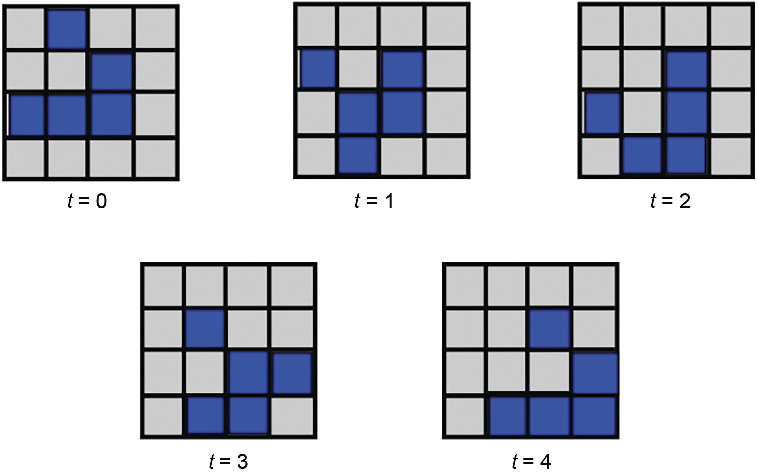
\includegraphics{graphics/Chapter_02/Figure1.pdf}}{Scheme of the translation of the ``Hello world!'' program from assembly code to hexadecimal code.}[-350pt,3pt]\vspace*{9pt}
\caption{\label{fig:2.1}The assembly instructions and the machine code of a very simple program that prints the string ``Hello world!'' An assembler program must be used to translate the original instruction to machine operations (here represented in a hexadecimal format).}
\end{figure}

Approximately ten years after the first production and use of digital \hbox{computers,} it was usual to implement software programs using assembly languages to avoid the hard-coding, error-prone, tedious, and time-consuming first-generation machine language programming used with the earliest computers, freeing programmers from keeping track of binary codes and data addresses. From a historical viewpoint, Kathleen Booth is recognized as the inventor of the first assembly language in 1947. In late 1948, David Wheeler developed the first assembler program for the EDSAC and integrated it into the computer bootstrap program. For around another ten years algorithms in digital computers were coded using assembly languages. However, by the late 1950s the use of assembly languages had been replaced by the so-called high-level languages---with the goal of improving programming productivity and guarantying portability of algorithms from one computer to another with a different CPU. Today, assembly languages are still used for direct hardware manipulation in modes unsupported by a higher-level language, programming specific embedded hardware systems, accessing specialized processor instructions, or solving critical performance issues. For example, in operating systems development, where from the early 1950s to the end of the 1960s most operating systems were entirely implemented using assembly languages, today only 1\% to 2\% of the operating system kernel code is written in assembly; the rest, that is, more than 98\%, is written in high-level languages such as C, C++, and Java.




It is worth mentioning that the assembly language of the \textit{Apollo Guidance\break Computer} (AGC) produced for the Apollo program and installed on board each Apollo command module and Apollo Lunar Module was the first programming language to land on the Moon. On July 20, 1969, the algorithms that managed and steered Apollo 11 landed on the Moon on board the Eagle lunar module together with Neil Armstrong and Buzz Aldrin. The software of the AGC contained about 145,000 lines of code and was implemented by a team of 350 programmers headed by Margaret Hamilton. She was the director of the Software Engineering Division of the MIT Instrumentation Laboratory, where the software for NASA's Apollo program was developed. Despite its complexity and very long list of instructions, bugs were never known to have occurred during any Apollo mission.

\section{\label{sec:2.5}High-level Languages, Concepts, and Evolution}

A simple way to classify programming languages is to divide them between low-level and high-level languages. Low-level programming languages provide little or no abstraction from a computer's instruction set architecture. Their instructions are very simple and hard to read (for humans). Machine languages and assembly languages belong to this class. Low-level languages can be considered as being close to the hardware operations and far away from human languages. Programs written in low-level programming languages do not provide a good abstraction from hardware and are generally non-portable from one system's architecture to another. Conversely, high-level programming languages provide abstraction from the details of the computer hardware and offer a way to express algorithms in a style similar to human languages. In fact, they use human language names, lexicons, and syntax, making the process of programming an algorithm easier, faster, and more readable than when a lower-level programming language is used. Different high-level languages provide diverse levels of abstraction that allow a programmer to be detached from the machine hardware details. The use of high-level languages in coding algorithms often results in lower performance because each high-level instruction must be translated (by a compiler or an interpreter) to a sequence of machine language instructions. However, the benefits in terms of productivity, portability, modifiability, and readability are so significant that they are the most used languages today.

A compiler is a program designed to translate code written in one high-level programming language (the ``source language'') into another language (the \hbox{``target} language''), typically low level (e.g., assembly language or machine code), to create an executable program that can be executed by a given CPU or a class of CPUs sharing hardware features. Among the main tasks of a compiler is to control the correctness of the source code through lexical, syntax, and semantic analysis and the production of the executable code. By contrast, an interpreter is a software program that analyzes each single instruction of a program (generally coded in a high-level language) and directly executes it without requiring it to previously have been compiled into a machine language program. If an instruction is incorrect, the interpreter stops the program execution, and the next instructions will not be executed. An interpreter generally uses different strategies for program execution as follows:

\begin{itemize}
\item Sequentially analyze the program source code and execute its instructions directly.

\item Translate code into an intermediate representation (or object code) and immediately execute that.
\end{itemize}

\noindent An interpreter can sometimes be used together with a compiler: for example, when pre-compiled intermediate code (i.e., bytecode) produced by a compiler is passed to an interpreter to be executed. In this case, the interpreter is able to read each bytecode instruction and execute it.

While programs were developed in machine or assembly languages in the first few decades of the computer age, today most software applications are implemented in high-level interpreted and/or compiled languages. The first commonly used high-level programming language was FORTRAN (FORmula TRANslator), a language designed in 1957 by a team led by John Backus at IBM. The FORTRAN language was developed for programming scientific, mathematical, and statistical algorithms, and, after more than 70 years and several extended versions, it is still in use today for programming and executing scientific applications. Before IBM developed the FORTRAN language, other high-level languages such as Plankalk\"{u}l (Plan Calculus), Short Code, and Autocode were designed and partially implemented, although they were not used by many programmers. Examples of  statements defined in FORTRAN and in the early high-level programming languages are the \texttt{IF} conditional statement, the \texttt{READ} and \texttt{WRITE} statements for input/{\allowbreak}output operations, the \texttt{GO~TO} jump unconditional statement, and the \texttt{DO} loop for executing a group of operations until a given condition becomes false. The use of these high-level statements improved the productivity of programmers in software implementation, simplified their programming tasks, and made the program code much more concise and easier to read. Two or three years after FORTRAN was introduced, other high-level languages such as ALGOL (Algorithmic Language), LISP (List Processor), and COBOL (Common Business-Oriented Language) were developed. In particular, the programming model used in ALGOL served as the basis for the development of some of the most important high-level programming languages including Simula, Pascal, C, C++, and Java.

In 1964, a team of students at Dartmouth College developed the BASIC \hbox{(Beginner's} All-Purpose Symbolic Instruction Code) language that ten years later was developed further by Bill Gates and Paul Allen and became the first marketable product of Microsoft. While BASIC used very simple programming instructions and structures that made it very easy to learn and use, not many checks were carried out by the compiler on its data abstractions and operations. As the years passed, several new programming languages were developed that allowed faster and more efficient production of software. In 1970, Niklaus Wirth developed \hbox{PASCAL,} a very well-structured programming language in honor of the French mathematician Blaise Pascal. In 1972 at Xerox Labs, Alan Key and his team implemented the Smalltalk language that introduced a set of programming concepts and mechanisms that are used today in languages such as Python, Java, and Ruby. Smalltalk was the first object-oriented language, that is, a language based on the concept of ``objects,'' which contain data (with their attributes) and code in the form of procedures (or methods). A common feature of objects is that methods are associated to them and only methods can be used to read and modify the object's data fields. This feature allows a more abstract way to implement software programs and verify their correctness. In the same year, Dennis Ritchie at Bell Telephone Laboratories worked on a new programming language for coding application and system programs and developed the C language. After implementing a compiler, together with Ken Thompson he used the language to implement the Unix operating system. The new language was called C simply because it was based on an earlier language called B. Some current leading languages such as C++, C\#, Java, JavaScript, Perl, PHP, and Python are in part derivatives of~C. 

\section{\label{sec:2.6}Source and Executable Code}

The collection of high-level programming languages is extensive and cannot be completely listed here. However, some other modern languages are Ada, Objective-C, Perl, Haskell, Visual Basic, JavaScript, Python, PHP, Ruby, Scala, Swift, and Go. For a quick and simple comparison of low-level languages, such as machine and assembly languages, with high-level languages, Figure~\ref{fig:2.2} shows the program code written in C language of the trivial ``Hello world!'' program that was introduced in Figure~\ref{fig:2.1}. In contrast to assembly statements that require deep programming skills, the very few statements of this C program can be read by non-specialists. In particular, after the \texttt{\#include} directive that is used to include in the program the input/{\allowbreak}output standard library---for allowing the printing of strings of text on the screen---and the \texttt{main()} statement that starts the operations, the C program uses only one statement (the \texttt{printf} function), whereas the machine and assembly programs in Figure~\ref{fig:2.1} use more than ten instructions to code this very trivial program.

\begin{figure}[!t]
\begin{tabular}{l}
\texttt{\#include <stdio.h>}\\
\texttt{main ()}\\
\texttt{\{}\\
\texttt{printf(``Hello World!'');}\\
\texttt{\}}
\end{tabular}
\caption{\label{fig:2.2}The C code of a program that prints the string ``Hello world!'' A C compiler is used to translate this program to machine instructions that will be executed by the language runtime.}
\end{figure}

To show how a high-level language allows programmers to code algorithms, we describe the C code of two algorithms introduced in Chapter~\ExternalLink{chap:1}{1}. The first one, shown in Figure~\ref{fig:2.3}, is the Euclid algorithm that finds the greatest common divisor of two positive integers \textit{a} and \textit{b}. The greatest common divisor of two numbers is the largest number that divides both. A simple method to find that divisor is to factorize both numbers and multiply common factors.


\begin{figure}[!b]
\begin{tabular}{l}
\texttt{\#include <stdio.h>}\\
\texttt{main ()}\\
\texttt{\{}\\
\texttt{int a, b, r;}\\
\texttt{scanf(``Insert the first value \%d'', \&a);}\\
\texttt{scanf(``Insert the second value \%d'', \&b);}\\
\texttt{while (b>0) \{}\\
\quad\texttt{r=a\%b;}\\
\quad\texttt{a=b;}\\
\quad\texttt{b=r;}\\
\texttt{\}}\\
\texttt{printf(``GCD is: ''a);}\\
\texttt{\}}
\end{tabular}
\caption{\label{fig:2.3}The C code of the Euclid algorithm that finds the greatest common divisor of two positive integers.}
\end{figure}


Let us use integer variables \textit{a} and \textit{b} to represent the two numbers and the variable \textit{r} to represent the remainder of their division, that is, \textit{r} is equal to \textit{a \% b}. After reading the two values by using the \texttt{scanf }function, the \texttt{while} loop is utilized to determine the remainder \textit{r} and assign current values of variables \textit{b} and \textit{r} to variables \textit{a} and \textit{b}, respectively. Please note that the symbol ``$=$'' used in the three operations into the while loop is the assignment operator used in C and in other languages to assign a value to a variable. The assignment operator is different from the equality operator that is expressed by a double equal sign ``${=}{=}$'' (see the program in Figure~\ref{fig:2.4}). Execution of the operations in the \texttt{while} loop is continued as long as the value of divisor \textit{b} is greater than zero. When the value of \textit{b} becomes zero, the value of variable \textit{a} is the GCD of the given numbers, and it is visualized by the \texttt{printf} statement.

In Chapter \ExternalLink{chap:1}{1}, we also introduced the simple linear search algorithm for finding a given value in a list of numbers. Here (see Figure~\ref{fig:2.4}), we show the C program that implements that algorithm. After reading the list of elements through the \texttt{for} loop, the program asks for the number to be searched \texttt{(scanf(``\%d'', \&x);)}, and then sequentially through the second \texttt{for} loop compares each element $S[i]$ with the element to search \textit{x} until it finds it and prints its position or the list ends, in this case the program signals that the number is not present in the list.

\begin{figure}[!b]
\begin{tabular}{l}
\texttt{\#include <stdio.h>}\\
\texttt{main ()}\\
\texttt{\{}\\
\texttt{int N = 100, S[N], x, i, j;}\\
\texttt{printf(``Enter \%d integers: '');}\\
\texttt{for (i = 0; i < N; i++)}\\
\qquad\texttt{scanf(``\%d'', \&S[i]);}\\
\texttt{printf(``Enter a number to search: '');}\\
\texttt{scanf(``\%d'', \&x);}\\
\texttt{for (i = 0; i < N; i++)\{}\\
\quad\texttt{if (S[i] == X) \{}\\
\qquad\texttt{printf(``\%d is at location \%d.'', x, i+1);}\\
\qquad\texttt{break;}\\
\quad\texttt{\}}\\
\texttt{\}}\\
\texttt{if (i == N)}\\
\quad\texttt{printf(``\%d is not present in the list \%d.'', x);}\\
\texttt{\}}
\end{tabular}
\caption{\label{fig:2.4}The C program implementing the linear search algorithm that, given an array of elements of size $N=100$, let find a given value \textit{x}, if it is within the array.}
\end{figure}


Although the C source code requires a few technical commands to be included (for instance, the \texttt{\#include} directive, the parentheses for grouping blocks of code, and some data format pragma such as \texttt{\%d}), the program is readable and understandable enough for non-experts. Source code in high-level languages is in fact a sequence of human-readable instructions that programmers write when they develop the program. Program code is then stored in files for further changes or for producing executable code by a compiler. When the source code is complete, it is run through a compiler to turn it into machine code called executable code. This is a program code that a computer can understand and execute but humans are no longer able to read and change appropriately because machine code consists of binary sequences of 1s and 0s that are not human-readable. While most high-level programming languages use a compiler-based approach to produce machine code, a few programming languages, such as JavaScript or PHP, are interpreted instead. In interpreted languages, the distinction between source code and executable code does not apply because there is only the source code that is analyzed and executed by an interpreter that processes each single instruction and, if correct, generates the corresponding machine code to be executed. Generally, application software is distributed in a form that includes only executable files. This means that we can install and run that software but we cannot modify or reuse it in other programs. If the source code of programs is included, it would be useful to a programmer or a systems developer who might wish to study and/or modify that code.

In this context, the concept of \textit{open-source} programs plays an important role. This term was coined in the field of software development to describe a specific approach to building and distributing computer programs. Today, however, the keyword ``open source'' describes a broader set of values, projects, products, and initiatives that include and celebrate principles of open exchange, collaborative participation, rapid prototyping, transparency, and community-oriented development. The open-source model is a decentralized software development and \hbox{maintenance} standard that encourage open collaboration among software programmers, teams, and companies. A main principle of open-source software development is peer production, with products such as source code, schemes, and documentation freely available to the public. According to this approach, the source code of programs is distributed together with the executable to allow users and programmers to learn the algorithms used in these software programs and modify/{\allowbreak}extend them if needed.

Open-source technology benefits both expert programmers and end-users. In fact, computer users prefer open-source software to proprietary software for several practical reasons, including control of the used algorithms, security in execution, readability, and training. Some open-source licenses require that anyone who releases a modified open-source program must also release the source code for that program. Furthermore, we must keep in mind that some licenses specify that who ever alters and shares an open-source program with others must also share that program's source code without charging a licensing fee for it.


\section{\label{sec:2.7}Software Applications}

The number of software applications that are used today in every moment and every aspect of our daily life is immeasurable. For every action we take at work or at home there is an application that may assist us. We can say that the relationship of human beings with reality is more and more often and more deeply regulated by algorithms, which encode billions of operations that are recorded in digital storage and executed by the CPUs of computers, smartphones, webcams, sensors, smartwatches, and many other digital devices. Application software, also known as end-user software or productivity software, include algorithms that perform specific personal, educational, and business functions. Each application is designed to assist end-users in accomplishing a variety of tasks, which can be linked to data processing, productivity, communication, traveling, or creativity. The most common software application platforms today are used by millions of people every day. Applications like Spotify, Chrome, Firefox, Zoom, Gmail, Word, and many others are designed to help with specific tasks that are increasingly vital for people.

The functions implemented by application software can be personal, business, as well as educational. Each software program is developed by using high-level programming languages to assist people with a particular process related to productivity, efficiency, or communication. The large number of apps that are installed on our smartphones are clear examples of application software. For over 6.5 billion smartphone users across the world, software apps have become their everyday companion and most software apps are becoming irreplaceable for many of us. As Statista (\href{https://www.statista.com}{www.statista.com}) reported, in the first quarter of 2021, ``Android users were able to choose between 3.48 million apps, making Google Play the app store with biggest number of available apps. The Apple App Store was the second-largest app store with roughly 2.22 million available apps for iOS.'' The average price of an app in the App Store amounts to US\$0.91. Other than Apple and Google, who dominate the app market, there are a few other players such as Amazon Appstore, offering about 500,000 Android apps to worldwide audiences, and the Tencent Appstore, with around 50,000 available apps as of 2022. This impressive scenario makes evident the very important role of algorithms, which through the exploitation of programming languages can be implemented as software programs and run very fast on billions of digital devices.


\begin{thebibliography}{}

\bibitem[Boole(1848)]{chap:02:Boole:1848} G. Boole. 1848. The calculus of logic. \textit{Camb. Dublin Math. J.} 3, 183--198.

\bibitem[Boole(2009)]{chap:02:Boole:2009}G. Boole. 2009. \textit{An Investigation of the Laws of Thought on Which Are Founded the Mathematical Theories of Logic and Probabilities}. Cambridge University Press, Cambridge.

\bibitem[Davis(2012)]{chap:02:Davis:2012} M. Davis. 2012. \textit{The Universal Computer: The Road from Leibniz to Turing}. CRC Press.

\bibitem[G\"{o}del(1931)]{chap:02:Godel:1931} K. G\"{o}del. 1931. \"{U}ber formal unentscheidbare S\"{a}tze der Principia Mathematica und verwandter Systeme I. \textit{Monatshefte f\"{u}r Mathematik und Physik} 38, 1, 173--198. DOI:~\href{https://doi.org/10.1007/BF01700692}{https://{\allowbreak}doi.{\allowbreak}org/{\allowbreak}10.{\allowbreak}1007/{\allowbreak}BF01700692}.

\bibitem[Neumann(1945)]{chap:02:Neumann:1945} J. v. Neumann. June 1945. \textit{First Draft of a Report on the EDVAC}. Moore School of Electrical Engineering, University of Pennsylvania.

\bibitem[Shannon's(1938)]{chap:02:Shannon:1938} C. E. Shannon. 1938. A symbolic analysis of relay and switching circuits. \textit{Trans. Am. Inst. Electr. Eng.} 57, 713--723. DOI:~\href{http://doi.org/10.1109/T-AIEE.1938.5057767}{http://{\allowbreak}doi.{\allowbreak}org/{\allowbreak}10.{\allowbreak}1109/{\allowbreak}T-{\allowbreak}AIEE.{\allowbreak}1938.{\allowbreak}5057767}.

\bibitem[Smith(2014)]{chap:02:Smith:2014} J. T. Smith. 2014. David Hilbert's radio address---German and English. Mathematical Association of America. [Online]. Retrieved June 10, 2022 from \href{https://www.maa.org/press/periodicals/convergence/david-hilberts-radio-address-german-and-english}{https://{\allowbreak}www.{\allowbreak}maa.{\allowbreak}org/{\allowbreak}press/{\allowbreak}periodicals/{\allowbreak}convergence/{\allowbreak}david-hilberts-{\allowbreak}radio-{\allowbreak}address-{\allowbreak}german-{\allowbreak}and-english}.

\bibitem[Turing(1937)]{chap:02:Turing:1937} A. M. Turing. 1937. On computable numbers, with an application to the Entscheidungsproblem. \textit{Proc. London Math. Soc.} s2--42, 1, 230--265. DOI:~\href{https://doi.org/10.1112/plms/s2-42.1.230}{https://{\allowbreak}doi.{\allowbreak}org/{\allowbreak}10.{\allowbreak}1112/{\allowbreak}plms/{\allowbreak}s2-{\allowbreak}42.{\allowbreak}1.230}.
\end{thebibliography}

%\end{document}


%\documentclass{acm-book-v2}
%\RequirePackage[errorshow]{tracefnt}
%%\newcommand{\mpage}[1]{}
%%\newcommand{\indexfn}[1]{}

%%\usepackage{showframe}

%\usepackage{custom-tooltip}
%\usepackage{custom-tooltip-Alt-Text-View}



%\begin{document}

\setcounter{chapter}{2}

\chapter{\label{chap:3}Algorithms and Data---{\allowbreak}The Pillars of Our Future}

This chapter examines the relationships and synergies between algorithms and data. In particular, we introduce and discuss data structures, databases, web data, and Big Data concepts. The data science discipline created for exploiting Big Data in scientific discovery is also introduced. Large data storing/{\allowbreak}management/{\allowbreak}processing by smart and efficient algorithms is also illustrated through practical use cases in significant application domains such as digital health, smart cities, social media, and science.

\section{\label{sec:3.1}Data Storing and Abstract Structures}

The Merriam--Webster dictionary defines data as ``factual information (such as measurements or statistics) used as a basis for reasoning, discussion, or calculation.'' This very basic and general definition recalls that data are a main element in reasoning and computation. A second definition given by that dictionary is more relevant to the field of computing we are discussing here: data is ``information in digital form that can be transmitted or processed.'' Although raw data, also in digital form, should be considered as simple units that compose information, this latter definition is very useful for understanding the importance of data for computers and algorithms. Without input data that express facts, symbols, words, and numbers, computers cannot produce any result and algorithms cannot execute their operations. Upon completion, the ENIAC computer had 20 accumulators that operated as computational and storage devices. Each accumulator could store one signed 10-digit decimal number. That was the original way to represent and store data in the pioneering electronic computer. At that time, the ENIAC had no main memory; only in 1953 was a 100-word static magnetic-memory added. It was based on a binary-coded decimal number system and can be considered as the progenitor of the random-access memory (RAM) used today in all computers and digital devices.

While the term ``data'' is now very often associated to the dictionary's second definition that we mentioned, this word is much older than computers. It comes from Latin where \textit{data} is the plural of \textit{datum} meaning ``(thing) given or granted,'' the past participle of \textit{dare}, ``to give.'' In English, this word was rediscovered in the 17th century from its Latin roots and used in statistical studies, engineering, and other scientific fields. In the first decades of the 20th century, scientists and engineers worked on techniques and devices for storing data and information. Among others, we should mention an Austrian engineer, Fritz Pfleumer, who invented a technique for storing information magnetically on tape. Pfleumer, who was an expert in industrial processes for producing special papers, used thin cigarette paper to create a coated paper recording tape by replacing the bronze with a magnetizable medium. He patented the first audio tape recorder, which piqued the interest of German General Electric (AEG) who a few years later signed a contract with Pfleumer and afterward produced the world's first practical tape recorder, called the Magnetophon K1. The principles Fritz Pfleumer developed are still used today, with the vast majority of digital data being stored magnetically on computer hard disks.

Without a significant amount of memory, a computer would merely be able to perform fixed operations and immediately output the result. It would have to be reconfigured to change its behavior. This could be acceptable for devices such as desk calculators, digital signal processors, and other specialized devices, but it is an unacceptable limitation for general-purpose computers. Machines based on the von Neumann architecture include a memory in which they store both instructions and data. By exploiting that memory, digital computers are versatile in that they do not need to have their hardware reconfigured for each new operation/{\allowbreak}program to be executed. That memory is used to store the instructions/{\allowbreak}programs and data they must process every time it is needed.

A computer includes different types of memory where data are stored, of which three are the most important and popular: main memory, secondary storage, and tertiary storage. Main memory is the fastest and the only one directly accessible by the CPU, which, when running a program, reads the instructions and data stored there. Whereas main memory is volatile, secondary storage is persistent in storing data. Hard disk drives or solid-state drives are usually used as secondary storage. They can store much more data than main memory, typically two orders of magnitude more. Secondary storage is less expensive but thousands of times slower than main memory. Finally, tertiary storage is sometime used for archiving very large rarely accessed data as it is much slower and cheaper than secondary storage.

While in human history the most commonly used data storage medium was the paper used in books, journals, newspapers, and other similar sources of \hbox{information,} in the last ten years the most used data storage media are magnetic, semiconductor, and optical devices. The current limited usage of paper has been caused by the very wide diffusion of computers and digital devices where data and information are mainly stored and circulated. A significant effort was carried out by computer designers and scientists to define and implement appropriate mechanisms and formats for storing and accessing data in computers. Other than implementing the different types of hardware memory devices, abstract data types and data structures have been defined to model and represent the conceptual organization, structuring, and operations associated with data stored in a computer.

A data type is a feature of data that defines the values it can take and the operations that can be performed on it. Therefore, a data type is a formal way to specify what to store and how to handle data. Programming languages support a set of basic data types such as byte, integer (to represent integer numbers), floating-point (for real numbers), characters, and Booleans (to represent the two truth values true and false). A data type is a very useful way to assign a meaning to each data item that is stored in a computer memory and will be processed by the CPU. It is a practical concept to express and limit the possible values and the operations that can be done on data. For example, the Java programming language defines basic data types that include \textit{byte}, \textit{short}, \textit{int}, \textit{long}, \textit{float}, \textit{double}, \textit{boolean}, and \textit{char}. One of them will be associated to each single data element (a variable or a data record) stored in computer memory. For instance, the following data declarations specify a numeric variable (named \textit{index}) and a character (named \textit{reply}):

\begin{center}
\texttt{\textbf{\MonoBold int} index};

\texttt{\textbf{\MonoBold char}} \texttt{reply};
\end{center}

\noindent Arithmetic operations can be executed on the integer \textit{index} that stores a 32-bit signed integer, which can take a minimum value of $-2{}^{31}$ and a maximum value of $2{}^{31}-1$. Typical operations used to operate on the character variable \textit{reply} are copy, print, and concatenate.

In general, languages, operating systems, and other software systems allow programmers and users to utilize sets of data structures for storing and processing their data, which may be built from the combination of basic data types. A data structure is a collection of data values that may be of different types, relationships among them, and operations that can be applied to its data elements. For example, non-primitive data types in Java that are used to implement complex data structures are \textit{String}, \textit{Arrays}, and \textit{Classes}. Most high-level programming languages also allow developers to define additional composite data types. This can be done by combining multiple elements of basic types and defining the new operations (through functions or methods) of the new data type. Examples of composite data types are array, lists, records, sets, and unions. An array is a fixed-length or resizable collection of elements in a specific order, typically all of the same type. Array elements are accessed using an integer index to specify which element is required.\break A list is a linear collection of data elements of any type, called nodes, where each node contains a value and a pointer to the next node in the list. A list is more flexible than an array because elements can be inserted and removed without relocating the rest of the list. A record is an aggregate data structure whose elements, called fields, can have different basic types. A record element, for example, may be composed of three fields: an integer, a string, and a Boolean. The set data type is an implementation of the mathematical concept of a finite set; thus, it is a data type that stores unique values without any particular order. Operations such as \textit{union}, \textit{intersection}, and \textit{subset} are defined on variables of the set type. Finally, the union data structure defines which of a number of permitted primitive types may be stored in its instances, for example, \textit{float} or \textit{short} integer. Unlike a record, which can contain a \textit{float} and an integer, a union stores only one value at a time. In its implementation, adequate memory space is allocated to contain the widest member\break data type.

Data structures provide a means to efficiently compose, store, and manage large amounts of data that can be used in complex software applications such as scientific simulations, file systems, databases, information retrieval systems, and web services. They are used to organize storage and retrieval of information kept in the different types of memories used in computers, in particular in the main or secondary memory. As the size and complexity of data increase, data structures play a very important role in the development of software systems and applications. Effective data structures are vital for developing efficient algorithms. The most recent programming languages emphasize the role of data types and data structures, with respect to algorithms, as the crucial organizing element in the design of scalable software systems. Smart storage mechanisms and strategies of data processing are vital for the development of large-scale applications and services that deal with distributed data repositories, as occurs in cloud computing infrastructures, in several application fields.

\section{\label{sec:3.2}Data in Files}

A very important abstract structure to store and manage data is provided by files. A file is a collection of data handled by a computer as a unit and identified by its name. Files are used for storing data in secondary or tertiary storage and for purposes of managing input and output. Files are stored on disks or magnetic tapes and represent the used data abstraction for keeping data persistent in computers. Indeed, data and information stored in a file survive the termination of the program using them or when the computer is switched off. Files can be shared with and transferred between computers via removable media or the Internet. A file can contain a few data elements (words, numbers, program code, etc.) or it can be very large up to gigabytes or terabytes of data. Files enable users and applications to save, read, write, and modify data; they use different internal structures that may also help to find the data that matches certain criteria. Different types of files are designed for different purposes. However, on most current operating systems, files are organized into one-dimensional arrays of bytes. This simple structure allows for encoding different data formats using an appropriate combination of characters to define, for example, GIF or HTML files. A file may store an executable program, an image, a short or long text document, a video, or any other kind of combined data elements. The main goal of developing file structures and organization is to minimize the number of transfers from the disk to the main memory and vice versa, limiting disk access as much as possible.

The word ``file'' is derived from the Latin \textit{filum}, in English a thread. In modern times, a file defines a collection of  papers or publications, one that is usually arranged or classified. After the development of computers, the term file has been used in the context of computer storage to define a collection of data archived on a digital storage device. From the early 1950s, this term denoted information stored on computer hardware devices, including punched cards, vacuum tubes, and disk drives. About ten years later, operating systems, such as the Compatible Time-Sharing System (CTSS) developed at MIT and the Master Control Program (MPC) implemented at Burroughs included a module devoted to managing files on storage devices that was called a file system. Today, all operating systems include one or more file systems that organize the way files are stored on hardware devices---how they are named, stored, and retrieved.

A file system consists of two distinctive parts: a pool of files, each one storing data, and a set of directories that organize and provide information about all the files in the system. Directories are abstract structures that connect and group files in folders (each folder is called a directory) that virtually represent a wrapper for files. Directories then allow a user to group files into separate collections. Originally, directory structures were flat. The first implemented file system supporting hierarchies of directories was the MULTICS operating system. All operating systems nowadays include file systems that define hierarchies (such as trees or graphs) where directories may contain sub-directories. For example, Windows uses the FAT32 and NTFS file systems while Linux uses ext3, FAT32, and exFAT. Although file systems are data structures devoted only to storing and accessing data in secondary storage, they play a very important role in the management of data. In the era of Big Data, new file systems for parallel computers and distributed systems, such as NFS, HDFS, Google File System, and GPFS, were developed and used to store very large amounts of information in files residing on different disks and for allowing a set of programs to access the information stored in files concurrently.

Distributed and parallel file systems are used today to store large amounts of data in files distributed across multiple networked computers and to enable fast access through simultaneous, concurrent input/output operations between software applications and storage servers. A high-performance file system splits a large file and distributes, or stripes, its portions to several storage drives, which can be located on different remote servers connected in a local area network or through the Internet. Users do not need to know the physical location of the partitions to read or modify a file as the system uses a global namespace to facilitate file access. Storage capacity and bandwidth can be scaled to store huge amounts of persistent data in files, and services may include high availability,  fault-tolerance, and replication.

\section{\label{sec:3.3}Data in Databases}

A big step in storing and
processing data has been the development of databases. A~database is a well-structured collection of data and information specifically organized for efficient search and retrieval by a computer. Databases are computer-based archives structured to facilitate the storage, retrieval, modification, and deletion of data carried out by a set of data-processing operations. Apart from storing the data itself, a database also includes the relationships among the data elements that enrich data and support complex retrieval operations. Data, structures, and relations of a database can be stored on a set of files. However, databases, through data abstractions and their relations, offer a more efficient and better structured model for storing and querying data. Databases are designed and implemented by using a database management system (DBMS), which is a software program that allow users to define, create, query, update, and maintain access to a database. DBMSs encompass all the core facilities that have been provided to generate and administer a database. When a database is in operation, a DBMS serves as the interface between users or their applications and the database, permitting data retrieval, updates, optimization, and the overall management of data and information stored in the database.

Early database management systems appeared in the 1960s, and they were designed and used in business sectors such as banking, airline ticketing, commerce, telecommunications, and in complex scientific projects such as the Apollo program for the Moon landing. The Integrated Data Store (IDS) was one of the first database management systems; it was designed in the 1960s at the computer division of General Electric and became the basis for the CODASYL Data Base Task Group standards. The CODASYL model offered software applications the capability to navigate around a linked dataset. They can find data records by using a unique key or navigating data relationships from one record to another or scanning all the records in a sequential order. For this reason, databases using this approach were called navigational databases. The CODASYL model became, for about ten years, the paradigm used for implementing commercial database systems such as the IDMS database from Computer Associates and the multidimensional MDBS2 database system.

When using the CODASYL model, designers realized that the internal data structures were not transparent, which required programmers to navigate database structures to obtain information (i.e., specify the access path, describing all of the records and the sets that would be used). This problem was solved in a new DBMS model called the relational model, invented in 1970 by Edgard F. Codd, a computer scientist working at IBM. Codd published a set of scientific papers where he described a new approach to database definition and implementation. The most well-known is ``A relational model of data for large shared data banks'' [\citealt{chap:3:Codd:1970}], where Codd wrote ``This paper is concerned with the application of elementary relation theory to systems which provide shared access to large banks of formatted data. {\dots} The relational view (or model) of data appears to be superior in several respects to the graph or network model presently in vogue for non-inferential systems. It provides a means of describing data with its natural structure only---that is, without superimposing any additional structure for machine representation purposes. Accordingly, it provides a basis for a high-level data language which will yield maximal independence between programs on the one hand and machine representation and organization of data on the other.''


In contrast to CODASYL, where data records are stored in some sort of linked lists, Codd proposed to structure data in a number of tables, each table being used for a different type of entity (e.g., employee, salary, job, and company). Each table would contain a fixed number of columns containing the attributes of the entity. For the employee entity, we may have attributes such as surname, age, city, school degree, and so on. One or more columns of each table were designated as a primary key by which the rows of the table could be uniquely identified. Primary keys are used for cross-references among tables and queries would join tables based on these key relationships using a set of operations based on the mathematical system of relational calculus (from which the model takes its name). Splitting the data into a set of tables (or relations) aimed to ensure that each item of information was only stored once, thus simplifying update operations.

After Codd's complete definition of the relational model, IBM worked on a prototype DBMS, called System R, which was based on those concepts. To manipulate and retrieve data stored in the System R database management system, Donald D. Chamberlin and Raymond F. Boyce developed the Structured Query Language (SQL) for programming and querying relational databases. SQL operations are based upon the relational algebra and tuple relational calculus used by Codd in his model. Among the programming concepts of SQL, the most important are \textit{queries}, which retrieve the data based on specific criteria, and \textit{statements}, which can have a persistent effect on schemata and data, or can be used to control transactions, program flow, connections, sessions, or diagnostics. An SQL query consists of three pieces, or blocks: the \textit{select}, \textit{from}, and \textit{where} blocks. The \textit{select} block tells the database which columns of data we want it to return. The \textit{from} block specifies which table(s) we want to search. The \textit{where} block allows us to search for records with certain characteristics. For instance, Figure~\ref{fig:3.1} shows the SQL query to be run if we want to retrieve all the names of people living in Rome who receive a salary of {\texteuro}100,000 or greater, from a database containing a table \textit{Persons} composed of five columns storing, respectively, the first name, surname, age, residence town, and salary of a list of people.

\begin{figure}[!b]
\begin{tabular}{l}
SELECT firstname, surname\\
FROM Persons\\
WHERE (town = `Rome') AND (salary >= 100,000)\\
\end{tabular}
\caption{\label{fig:3.1}An example of a simple SQL query on a relational database containing the table \textit{Persons }for retrieving the names of people living in Rome and receiving an annual salary higher than {\texteuro}100,000.}
\end{figure}

After the implementation of this relational DBMS, others such as INGRES, \hbox{Oracle} Database, and PostgreSQL were implemented and intensively used in the late 1970s. Examples of other well-known and widely used relational database systems developed in the 1980s are IBM Db2, MySQL, PostgreSQL, Microsoft SQL Server, and Microsoft Access. Indeed, by the early 1990s relational systems dominated all professional and significant data management applications. Moreover, as of the first two decades of the 2000s, they remain dominant, and the SQL database language for the relational data processing has influenced other database languages based on different data models. Among them are the object databases designed in the 1980s to overcome the difficulties of object--relational impedance mismatch, encountered when a relational RDBMS is being served by an application program written in an object-oriented programming language, such as Java or C++, because objects or class definitions used on object-oriented programs must be mapped to database tables defined by a relational schema. In some cases, the solution of this problem led to the development of hybrid object--relational databases.

The post-relational database systems in the late 2000s became known as NoSQL (for Not only SQL). Those database systems introduced fast key--value stores, graph-oriented, and document-oriented databases. They provide data models and mechanisms for storage and retrieval of data that are different from the tabular relations used in relational databases. The main goal of these new database management systems is to implement scalable databases in parallel and distributed computers for supporting Big Data applications that need to access and query very large datasets. The term NoSQL was coined around the year 2000 and in the succeeding years some NoSQL systems were developed mainly by private companies such as Amazon, Facebook, and Google and by open-source communities such as those working in the framework of the Apache Foundation, a non-profit corporation that supports several hundred open-source software projects. For example, in 2007 Amazon introduced its Dynamo distributed NoSQL system for internal use that was the inspiration for the implementation of the DynamoDB database service that supports key--value and document data structures. In fact, Amazon was one of the first big companies to store much of its important corporate data in non-relational databases.

As mentioned previously, different NoSQL database systems use different data models and methods. Their main advantages are that they can efficiently manage unstructured or semi-structured data such as social media posts, emails, videos and pictures, document files, geographical points and metadata, and other formats. NoSQL database systems are designed and used mainly for storing and querying unstructured data in efficient ways that require scalability when large amounts of data must be handled. Indeed, with relational databases users must convert all data into tables, and when the data doesn't easily fit into a table, the database's structure can be complex and slow to work with [\citealt{chap:3:Leavitt:2010}].

Several types of NoSQL database systems have been developed in the past 20 years; some of them overlap. Some of the most widely used are document-oriented, key-value, graph-based, and column-oriented databases. Document-oriented databases store and manage data as collections of documents rather than as tables having uniform-sized fields for each record. In document-oriented databases, users can define any number of fields of any length to a document. CouchDB is an example of this class; it was developed by the Apache Software Foundation as an open-source database system. MongoDB, RavenDB, and IBM Domino are other well-known document-oriented database systems. Key-value store database systems store data indexed for retrieval by keys. These systems can manage structured or unstructured data. They store the data as a single dense collection that may have different fields for every record. Using this unstructured approach, they need far less memory than relational systems to store databases, which can lead to performance gains. For example, Couchbase Server is a key-store system designed to provide scalable key-value and JavaScript Object Notation (JSON) document access. It is designed to be configured on a single computer or on several distributed servers when it needs to be used to store Big Data repositories.

Graph databases were designed by exploiting the mathematics of graphs, which models relations between entities that are represented as a set of vertices connected by edges. They use graph structures for semantic queries with nodes, edges, and properties to represent and store data. A graph database consists of a set of objects---each one can be a vertex (or node), an edge, or a property. Nodes represent data entities. They are comparable to a record, relation, or row in a relational database, or to a document in a document-store database. Edges connect a node to other nodes and represent the relationship between them. Edges are then the key concept in graph databases, representing an abstraction that is not directly implemented in a relational model or a document-store model. Properties are attributes associated to nodes. For example, if \textit{person} were one of the nodes, it might be associated to properties such as \textit{man}, \textit{age}, and \textit{home address}. Apache Giraph and Neo4j are two well-known graph database management systems.

Lastly, column-oriented databases store data tables by column rather than by row. They contain columns of closely related data rather than, as in relational databases, storing sets of data in a structured table of columns and rows with uniform-sized fields for each record. This structure assures more efficient data access when only querying a subset of columns and more choices for data compression. However, data insertion is typically less efficient. HBase is a distributed, open-source column database developed by the Apache Software Foundation that emulates Google's Big Table. Facebook created the high-performance Cassandra DBMS to store data from its social media platform.

Overall, we can say that NoSQL database systems are flexible enough to better enable developers to design databases in a way that meets their needs. In fact, NoSQL databases are often faster than relational ones because their data models are simpler. They don't have all the requirements that relational databases have. For example, they relax data consistency constraints that require the data values in the different copies of a data store to be kept consistent, enabling better performance and scalability for certain classes of applications. For more traditional applications, NoSQL databases won't replace relational ones. However, the many NoSQL solutions allow users to look at their data and select the most \hbox{appropriate} database management system they need, finding the best tradeoff between functionality and performance.

\section{\label{sec:3.4}Data in the Web}

Despite the big effort by database experts and users to model and organize data in a very structured way and provide efficient query mechanisms for finding the right information stored in those systems, in the early 1990s a momentous event significantly changed the path of computer data storing and processing technologies. In the 1960s, the American scholar Theodor H. Nelson introduced the hypertext concept as text shown on a computer display with references, called hyperlinks, to a number of other texts that a reader can directly access. This concept can be considered as a particular application of the hypergraph mathematical structure, which is a generalization of a graph in which an edge can link any number of vertices. In December 1968, Douglas C. Engelbart demonstrated at Stanford Research Institute the first hypertext software interface. From then until the end of the 1980s, several hypertext software systems were implemented and run on traditional sequential computers. Let us consider that when stored on a computer hypertext documents are interconnected by software hyperlinks, which are typically activated by a mouse click, a screen touch, or pressing a key on the keyboard. Hypertexts are often used to link plain or formatted text, tables, images, videos, and data of different formats.

The real change in the exploitation of hypertext systems occurred in 1989 in Geneva, where Tim Berners-Lee, an English computer scientist working at CERN, proposed and implemented a new distributed hypertext system for addressing the need for a simple information-sharing facility raised by physicists working at CERN and connected to many research centers and universities in the world. Tim Berners-Lee called the project ``WorldWideWeb.'' It was the first time that someone proposed to connect hypertexts with the Internet, which had already existed for around 20 years. Through this intelligent combination, Berners Lee created the web, the most used Internet service that offered a very simple interface to access the largest source of data and information created by humans and stored on billions of computers. ``Most of the technology involved in the web, like the hypertext, like the Internet, multifont text objects, had all been designed already. I just had to put them together. It was a step of generalizing, going to a higher level of abstraction, thinking about all the documentation systems out there as being possibly part of a larger imaginary documentation system'' [\citealt{chap:3:Berners-Lee:1990}].

On December 1990, Berners-Lee published the first website that was accessible to the Internet from the\vadjust{\vspace*{12pt}\pagebreak} CERN network. That website provided an explanation of what the World Wide Web (WWW) was and how people could use a browser or set up a web server. The WWW grew very quickly and after about thirty years the estimated active websites were about 1.2 billion, containing more than 50 billion web pages. As a curiosity, in June 2021 the web's source code developed by Berners-Lee was auctioned by Sotheby's in London and sold for US\$5,434,500 to fund benefit initiatives by him and his wife. As declared in the Sotheby's website [\citealt{chap:3:Sotheby:2021}], it includes the ``Original archive of dated and time-stamped files containing the source code, written between 3 October 1990 and 24 August 1991. These files contain code with approximately 9,555 lines, the contents of which include implementations of the three languages and protocols invented by Sir Tim; HTML (Hypertext Markup Language); HTTP (Hyper Transfer Protocol); and URIs (Uniform Resource Identifiers), as well as the original HTML documents that instructed early web users on how to use the application.'' This description contains an error in the HTTP explanation. Indeed, it is not the ``Hyper Transfer Protocol,'' but the Hypertext Transfer Protocol defined by Berners Lee as the application protocol for the distributed and collaborative exchanging of hypertext documents that composed the web pages. Together with it and the syntax of URIs, which are unique sequences of characters that identify resources used by web technologies (i.e., web pages), the third pillar of the web infrastructure is the HTML language.

HTML is the standard markup language for composing hypertext documents designed to be downloaded from a website and displayed on a web browser. The HTML components, including tags, text-based data types, characters, and entity references, have been defined to describe the structure of a web page. HTML tags, tables, images, videos, and other objects may be embedded into a rendered page. Therefore, HTML provides a linguistic tool to create structured documents by composing hypertext elements such as headings, paragraphs, lists, links, quotes, and other elements. HTML elements are delineated by tags, written using angle brackets. Tags such as $<$img$>$, $<$link$>$, and $<$table$>$ directly introduce content objects, such as images and tables, and hyperlinks into a web page. Other tags such as $<$p$>$ and $<$br$>$ are used to format document text and may include other tags as sub-elements. Web browsers are able to read and interpret the HTML source pages and visualize content of a page in a graphical format.

From the point of view of data storage and representation, HTML defines many data types as specializations of character data. They include script data, stylesheet data, names, URIs, numeric values, language types, media descriptors, colors, character encodings, dates and times, and many others. Following this approach, the web soon became the main repository of unstructured and semi-structured data, making it difficult to automatically process and query the great vastness of its billions of pages. In particular, semi-structured data stored in web pages do not follow the tabular structure of data stored in relational databases or other data structures used in NoSQL databases. In semi-structured data repositories, data items belonging to the same class can have different attributes even though they are grouped together and the order of attributes is not significant. The combinations of semi-structured and unstructured data have increased since the advent of the web and require different and new ways to browse, extract, pre-process, and analyze web data with respect to those stored in databases. For this reason, new markup languages such as JSON and Extensible Markup Language (XML) have been developed together with new techniques and algorithms for data processing such as web crawlers or spiders and web data scrapers. With the advent and extensive use of social media, the use of these techniques has been extended from web pages to the extraction and organization of social data items such as posts, tweets, and likes that billions of users publish on social media platforms.

Although database specialists have worked to design and implement techniques and systems for the management of well-structured data, the very wide use of Internet services and applications, and in particular the web and social media, has led to the creation of very large amounts of data stored on our computers and in the cloud in semi-structured and unstructured formats that are more complex to access and manage.

\section{\label{sec:3.5}The Era of Big Data}

The World Economic Forum estimated that at the beginning of 2020 the number of bytes in the digital universe was 40 times bigger than the number of stars in the observable universe. According to the Statista Research Department, the total amount of data created, stored, and exchanged globally in 2020 reached about 65 zettabytes, which is $65\times10{}^{21}$ bytes, or 65 billion terabytes. This extraordinary number is forecast to increase rapidly, and in 2025, the total amount of data stored in our computers and digital devices around the globe is projected to grow to about 180 zettabytes. The Statista specialists reported that the growth of data was higher than previously estimated because of the COVID-19 pandemic, since more people worked and studied from home and used home entertainment services more often. More than 90\% of data available in the world was generated within the past ten years. From 2020 to 2025, the IDC forecasts new data creation to grow at a compound annual growth rate of 23\%, resulting in approximately 175 zettabytes by 2025, a value that is similar to the Statista forecast.

Some people contend that data are the oil of the third millennium. Actually, data have created an immense market that is reaching impressive values. According to the research report ``{`Big Data Market'} information by technology, by organization size, by deployment, by end-user and region---forecast to 2030'' by Market Research Future, the data market size will reach US\$297.28 billion, growing at a compound annual growth rate of 14.52\% by 2030. By 2025, more than a quarter of data created will be real time in nature, and Internet of Things (IoT) real-time data will represent over 95\% of it. Actually, data are present wherever there is a memory device: in the disks of our computers, in smartphones, on the web, in social networks, in the private and public cloud platforms, in sensor networks, in digital cameras, in laboratory instruments, and in IoT devices. They are Open Data, Personal Data, Hyperdata, Linked Data, and other data models that will come in time. As mentioned, data hold a great economic potential and are responsible for creating the most valuable brands in the world such as Google, Facebook, and Amazon. Companies and organizations who will exploit data by analysis and learning tools will be able to benefit from a better understanding of phenomena, processes, behaviors, and trends. The IDC estimates that the amount of data subject to data analysis will grow by a factor of 50 to 5.2 zettabytes in 2025. However, these numbers say that a very small percentage of available data is used as input source for data analysis and machine learning tasks, thus dispersing most of its value.

Many definitions have been proposed for the Big Data term. Most of them, however, refer to the main features identified by Doug Laney, an analyst of the META Group, now Gartner, in its report published in 2001: large volume, high velocity, and large variety [\citealt{chap:3:Laney:2001}]. The term Big Data was not actually used in the Laney report; however, he clearly identified the rising trend of large repositories of data stored on digital devices and the ``management challenges along three dimensions: volumes, velocity, and variety. \dots\ In 2001/02, IT organizations must compile various approaches to have at their disposal for dealing with each.'' In more detail, Big Data refers to massive, heterogeneous, and often unstructured digital content that is difficult to process using traditional data management tools and techniques. The definition provided by the Gartner glossary is as follows: ``Big Data is high volume, high velocity, and/or high variety information assets that demand cost-effective, innovative forms of information processing that enable enhanced insight, decision making, and process automation.'' The NIST Big Data Public Working Group added variability as a fourth dimension [\citealt{chap:3:NIST:2015}] and wrote that ``Big Data consists of extensive datasets---primarily in the characteristics of volume, variety, velocity, and/or variability---that require a scalable architecture for efficient storage, manipulation, and analysis.''

Volume is about the impressive amount of data produced, stored, and exchanged through the Internet. As computers, networks, and human interactions on digital systems generate data, the volume of available data today is massive. Data velocity deals with the pace at which data flow in from their many sources. The flow of data on the Internet is continuous and extremely fast. Variety refers to the several different sources and types of structured and unstructured data. In the past, we used to store data from sources such as spreadsheets and databases; now data are generated through web pages, emails, social posts, photos, likes, PDFs, memes, videos, and voice recordings. This variety of data presents complications for collecting, storing, and analyzing digital data. Another characteristic that has been considered for Big Data is veracity, which deals with how accurate or truthful a dataset can be and includes how trustworthy the data source, type, and processing of it is. Therefore, dealing with data veracity also means removing bias, errors, inconsistencies, and null values.

While we need to deal with the proliferation of databases, web portals, audio and video streams, tweets, posts, and blogs that generated the Big Data phenomenon, we should recognize that data themselves are not necessarily important per se. Data become very important when we are able to extract value from them, thus adding a new ``V'' to Big Data properties: value. This new feature is obtained by reducing data volume and by identifying patterns, trends, and hidden information in large data repositories that may bring value to analysts and users. Big Data are the ideal companions for data analysis algorithms that without data could not compute results, make decisions, and solve problems. They represent very precious collections of contexts to be deciphered, hypotheses to be exhibited, and incessant traces that are very useful for people who know how to use them, for experts who are capable of sophisticated computations and, when necessary, of acute manipulations.

The Big Data scenario required a shift in data processing architectures from traditional systems based on vertical scaling, which exploit faster processors, main memory, or disks, to horizontal scaling, which can be implemented by adding more processors, computers, or machines to be used concurrently for running in parallel several programs/{\allowbreak}threads that may analyze different partitions of data simultaneously. This parallelization strategy in the past was mainly used for computationally intensive applications in scientific simulation and modeling; now it has been extended to data analysis and has created a new research and development field called high performance data analysis. Through the splitting and mapping of algorithms and data across independent processors, data scientists can greatly improve Big Data analysis, both managing very large datasets and reducing global processing time. Big Data analysis needs parallel computing infrastructures such as HPC systems, cluster computers, and clouds to run parallel algorithms for scaling data processing across a large number of storage and computing resources.

Big Data computing considers the world as the biggest digital laboratory. The task, which appears increasingly evident, is to compute real phenomena by exploiting those gigantic amounts of data, thus offering professionals, research teams, companies, and organizations extraordinary new opportunities. Nevertheless, it contains within itself the risk of marginalizing the processes and decisions related to actual quality, to the real meaning of things. To avoid this purely measurable horizon, the use of Big Data necessarily requires that we focus on the description of qualitative and not only quantitative elements of life and of natural phenomena.

\section{\label{sec:3.6}Data Science}

The Big Data phenomenon has prompted the
scientific community to reexamine research methods and processes by reorienting them toward insights obtained from the analysis of data. In 2007, Jim Gray, a Turing Award winner, addressed the separation of data-intensive science from computational science. He called for a paradigm shift in the computing architecture and large-scale data processing platforms known as the Fourth Paradigm [\citealt{chap:3:Heyetal:2009}]. Experiments, study of theorems and laws, and simulation were in chronological order in the previous three scientific paradigms. Tony Hey and co-authors argued that this new paradigm not only represents a shift in the methods of scientific research but also a shift in the way people think. He declared that the only way to deal with the challenges of this new paradigm is to build a new generation of hardware and software systems to efficiently manage, analyze, and visualize large amounts of data produced by this impressive data deluge. Stimulated by continuous and extraordinary advancements in processing power, communication bandwidth, storage, and an unprecedented wealth of data, Big Data processing solutions based on scalable algorithms and large datasets were developed to deal with the increasingly complex data science tasks.

The intensive use of computers, algorithms, and Big Data for scientific discovery processes has led to the development of \textit{e-science}, in which scientific methods have changed significantly through the use of computational methods and new data management and analysis strategies. A thousand years ago, science was empirical, and its main goal was describing natural phenomena. A few hundred years ago, the theoretical branch was born, which started to use models and generalize. Thanks to computers, in the last century a computational branch of science was created based on simulation of complex phenomena. Today, e-science unifies theory, experiments, and simulations to support data-intensive scientific discovery. Very large sets of data are produced and shared through digital machines and instruments or are generated by simulators. They are then processed by data analysis or machine learning techniques, and the information/{\allowbreak}knowledge they produce is stored in computer archives and on the Internet. In e-science, frameworks specialists analyze data using data science methods, powerful computers, and large-scale distributed platforms. The final paragraph of the edited version of the last talk by Jim Gray included in \textit{The Fourth Paradigm} [\citealt{chap:3:Heyetal:2009}] summarizes in a very clear way how computing changed science: ``I wanted to point out that almost everything about science is changing because of the impact of information technology. Experimental, theoretical, and computational science are all being affected by the data deluge, and a fourth, `data-intensive' science paradigm is emerging. The goal is to have a world in which all of the science literature is online, all of the science data is online, and they interoperate with each other. Lots of new tools are needed to make this happen.''

A very recent key discipline for this new paradigm that supports scientific discovery by the intensive use of computers, algorithms, and data is \textit{data science}. Data science combines computer science, applied mathematics, and data analysis techniques to provide insights based on large amounts of data. Data science improves discoveries by founding decisions on insight extracted from large datasets through the use of scalable algorithms for collecting, cleaning, transforming, and analyzing (Big) data. Although data science is a young discipline, its history began in the 1960s. In 1966, Peter Naur coined the term ``Datology'' as the ``science of nature and use of data,'' and in 1974, he used the term data science as the ``The science of dealing with data, once they have been established, while the relation of the data to what they represent is delegated to other fields and sciences.'' However, the first scientific conference mentioning data science in its name was the IFCS Conference in Data Science, Classification, and Related Methods held in 1996. Seven years later, the \textit{Journal of Data Science} was established to advance and promote data science methods, computing, and applications in all scientific fields.

In data science, algorithms play the same role that equations play in mathematics. Data gathering and collection is the first step in a data science process; however, it is not limited to the traditional data collection performed in statistics. Data science not only uses traditional data collection methodologies but it also uses data that are already available; that is, data produced for other goals that are accurately selected and pre-processed can be used for the analysis of scientific and business processes. In general, having more data helps. However, having the right data is the most important requirement. For this reason, most of the time spent in the data science processes (around 60--70\%) is for collecting and preparing data. In his survey on data science, Longbing Cao summarized the most used definitions for data scientist [\citealt{chap:3:Cao:2017}]. The US National Science Board defines data scientists as ``the information and computer scientists, database and software engineers and programmers, disciplinary experts, curators and expert annotators, librarians, archivists, and others, who are crucial to the successful management of a digital data collection.'' A report from the US Committee on Science of the National \hbox{Science} and Technology Council defines data scientists as ``Scientists who come from information or computer science backgrounds but learn a subject area and may become scientific data curators in disciplines and advance the art of data science. Focus on all parts of the data life cycle.'' Finally, the Joint Information Systems Committee defined data scientists as ``people who work where the research is carried out, or, in the case of data center personnel, in close collaboration with the creators of the data and may be involved in creative inquiry and analysis, enabling others to work with digital data, and developments in data base technology.''

A Venn diagram proposed by Drew Conway (see Figure~\ref{fig:3.2}) is often used to describe the overlapping skills needed by data scientists. The Mathematics and Statistics sphere includes knowledge of methods and tools such as probability theory, algebra, and stochastic analysis. The diagnosis of the problem is performed by applying various mathematical and statistical approaches to the available data. Math expertise is important because it helps scientists choose the correct procedure to solve their problems depending on the data they have. The Computer Science sphere refers to coding and programming skills needed for gathering and preparing the data and for applying learning and statistics algorithms to the problems. Finally, the Domain Expertise sphere completes the required skills as it implies the knowledge of the particular field in which people are working. Data scientists must know about the goals of that field, several methods, and the constraints that they will be dealing with.

\begin{figure}[!b]
\tooltip{\includegraphics{graphics/Chapter_03/Figure2.\image}}{Venn diagram showing three intersecting circles, one labeled Computer Science, another labeled Math \& Statistics, and the third one labeled Domain Expertise. The area of intersection is labeled Data Science.}[-240pt,-280pt]
\caption{\label{fig:3.2}The data science Venn diagram. It is based on the combination of three set of skills that contribute to provide the needed expertise of data scientists.}
\end{figure}

Data science processes aim to transform a problem into a solution by exploiting data, computational techniques and infrastructures, and analysis techniques. Typically, a data science process includes a set of steps as follows:

\bgroup
\def\labelenumi{(\arabic{enumi})}
\begin{enumerate}
\item \textit{Framing the problem}---Understanding and formalizing a problem will help data scientists build an effective model that can be appropriate and successful. At the end of this step, all of the information and context needed to address and solve the problem must be acquired.

\item \textit{Collecting the needed data}---This step involves realizing what data are needed and finding ways to gather that data from one or more sources such as file systems, databases, data warehouses, data repositories, social media, and web pages.

\item \textit{Processing the data for analysis}---This step is used to pre-process and clean raw data to ensure that the data is in the correct format for the analysis step. Inconsistencies and errors must be identified and dealt with appropriately.

\item \textit{Exploring the data}---Exploratory data analysis looks at and analyzes datasets and summarizes their main features. This step defines how to process and represent data, making it easier for data scientists to discover patterns, identify anomalies, or test hypotheses.

\item \textit{Performing in-depth analysis}---This step aims to produce the data model. Data mining, machine learning, statistical techniques, and mathematical algorithms are used to extract insights and predictions from data. Predictive and/or descriptive data models are eventually produced.

\item \textit{Communicating results of the analysis}---The final step is carried out to describe the results of the entire process. Proper communication in data science processes will put into action the discovered models and solutions of the addressed problem. Thus, communicating the findings in a clear way will highlight their value.
\end{enumerate}
\egroup

A major issue to be faced in the data exploration, processing, and analysis tasks used in data science applications is the time-consuming process of identifying and training an adequate model. Therefore, data science is a highly iterative exploratory process where most scientists work hard to find the best model or algorithm that meets their data challenge. In practice, there is no one-model-fits-all solution. Indeed, there is no single model or algorithm that can handle all dataset varieties and changes in data that may occur over time. All data analysis and machine learning algorithms require user-defined inputs to achieve a balance between accuracy and generalizability. This task is referred to as parameter tuning; it is a long and complex process that must be managed.

As we already mentioned, distributed systems, clouds, and HPC infrastructures provide the appropriate computing systems that underpin Big Data analysis by exploiting parallel programming algorithms and tools. Multidisciplinary skills and knowledge in both scalable computing and data science help to unlock the knowledge contained in the increasingly large, complex, and challenging datasets that are now generated across many areas of science and business. The integration of scalable computing resources, software tools, networking, data, information management, and expertise of data scientists using machine learning and data analysis algorithms provides the required combination for solving new problems and building new scientific disciplines around data.

The world is progressively moving toward a data-driven society where data are the most valuable asset. The proliferation of Big Data and big computing have boosted the adoption of machine learning and data science across several application domains. Efficient and optimized distributed and parallel in-memory and disk-based computing platforms for complex data analysis jobs are crucially required to tackle this challenge. Moreover, data science and data-oriented programming languages are needed to provide complex abstract structures and operations that must be close to problem formulation and data format and organization. Exploitation of efficient machine intelligence and data analysis is of great importance for solving complex and challenging problems. In this way data science is creating a new age of discovery.

\section{\label{sec:3.7}Data-intensive Applications}

Different studies report that in 2020 more than 2.5 quintillion bytes of data were generated every single day. People exchanged about 306 billion emails per day in 2020 while 294 billion were sent in 2019. In 2020, 3.5 billion searches were made on Google; in 2021, the searches were about 6 billion. In 2020, 432,000 hours of video were uploaded on YouTube per day, whereas in 2022 YouTubers uploaded around 720,000 hours of video content per day. These are just a few examples of the data deluge we are experiencing.

Because of this continuous and explosive growth of data, many data-intensive applications require exploiting scalable data storage and data analysis solutions. A well-known example of a Big Data application is the ATLAS detector at the Large Hadron Collider at CERN in Geneva. The ATLAS infrastructure has a capacity of 200 petabyte of disks and 300,000 cores, with more than 100 computing centers connected via 10 gigabits-per-second links. The data collection rate is very high and only a portion of the data produced\vadjust{\vspace*{-18pt}\pagebreak} by the collider is stored. Several teams of \hbox{scientists} run complex applications to analyze subsets of those huge volumes of data. The collection and analysis tasks would be impossible without a high-performance infrastructure that supports data storage, communication, and parallel processing. Also, computational astronomers are collecting and producing larger and larger datasets each year that without scalable infrastructures cannot be stored and processed. One significant example is the Energy Sciences Network (ESnet), the US Department of Energy's high-performance network managed by Berkeley Lab, which in late 2012 rolled out a 100 gigabits-per-second national network to accommodate the growing scale of scientific data. From 1990 to 2019, ESnet's average traffic has grown by a factor of 10 every four years.

If we go from science to society, social data and e-health are good examples to examine. Social media platforms, such as Facebook, Instagram, TikTok, and Twitter, have become very popular and are receiving increasing attention from the research community because, through the huge amount of user-generated data, they provide valuable information concerning human behavior, habits, and travels. When the volume of data to be analyzed is of the order of terabytes or petabytes (billions of tweets or posts), scalable storage and computing solutions must be used, but no clear solutions exist today for the analysis of very large datasets. The situation is the same in the e-health domain where huge amounts of patient data are available and can be used for improving therapies, for forecasting and tracking of health data, and for the management of hospitals and health centers. Very complex data storage and analysis in this area will need novel hardware and software solutions.

The widespread diffusion of sensors, webcams, and mobile devices and the availability of networking infrastructures is enabling the collection of big and heterogeneous data that are produced daily in urban spaces and the development of smart city services. Such data pertain to the mobility of people or vehicles, air quality, safety issues, water/electricity consumption, and so on. They represent useful resources for improving urban services and environments. This is stimulating the implementation of several applications and systems in the field of urban computing, an interdisciplinary scientific field that pertains to the study and application of computing technology in urban environments. The smart city paradigm aims to plan and design future urban territories in a more efficient way. Smart cities rely on the adoption of sensing technologies, databases, IoT systems, ubiquitous devices, wireless networks, and all those frameworks that are used for sensing cities and territories, for collecting data, and for acting on the basis of the application's logic. In order to process the large amount of data being produced, smart city applications are supposed to use multiple hardware and software technologies including parallel system architectures and clouds. Due to the specific nature of smart city software solutions, data and\vadjust{\vspace*{-18pt}\pagebreak} objects are strictly related to the space or territory in which they are defined and used. Indeed, environmental information extracted from sensors, data inherent to the neighborhoods and residential units in a city, and information about traffic and mobility are specifically descriptive of the city area where they have been gathered and stored.

The innovative organization of smart cities is one of the most important application scenarios where Big Data management is combined with IoT technologies. The main challenge is to harness the collaborative power of networks (networks of people, of knowledge, and of sensors) and use the resulting data and collective intelligence to implement better-informed decision-making processes and empower citizens, through participation and interaction, to adopt more sustainable individual and collective behaviors and lifestyles. For example, the collection of mobile phone data and the discovery of mobility models is one of the most challenging issues in urban computing and can help achieve several smart city objectives. Transportation analysis based on mobile phone data can be applied for \hbox{estimating} road traffic volume and transport demands, to forecast the public's future demand for taxis, or infer the origins of tourists and visitors. \hbox{Analysis} tasks can identify collective movement patterns to support city managers in transport planning, intelligent traffic management, route recommendations, and smart parking services. We can also mention infotainment applications that provide community services (e.g., point-of-interest notifications, electronic and financial services, media downloading, and parking zone management). These applications are built by the transmission, collection, and analysis of a huge amount of data exchanged among people and road units and are very useful for an efficient provisioning of such services.

The array of business and scientific activities that currently use very large amounts of data is very numerous and every day new applications are added to the list. For example, banking and securities are among the top business sectors using Big Data. The securities industries rely on Big Data for risk analytics, anti-money laundering, demand enterprise risk management, and fraud mitigation. Retail traders, banks, hedge funds, and other companies operating in the financial markets use Big Data for high-frequency trading, card fraud detection, archival tracking of audit trails, enterprise credit risk reporting, pre-trade decision-support analytics, sentiment measurement, and predictive analytics.

If we move to the scientific field, one of the latest extreme data applications is provided by the James Webb Space Telescope(JWST), which is already changing humanity's knowledge of the universe. The JWST is a large infrared telescope launched on an Ariane 5 rocket from French Guiana on December 25, 2021. It is a major optical telescope in space, and it has an approximately 6.5-meter primary mirror. The JWST will be the chief observatory of the next decade, providing data to thousands of astronomers worldwide. It will be used to study every phase of the history of the universe, ranging from the first luminous glows after the Big Bang to the formation of solar systems like our own, with a planet capable of supporting life.

The telescope is parked in a point of gravitational equilibrium located about 1.5 million kilometers beyond Earth. Being so far away from our planet means that the data it sends has a long way to travel to reach us correctly. It also means that the communications subsystem needs to be reliable and fast. The data collection and transmission rates of the JWST overshadow those of the older Hubble telescope. The JWST can produce up to 57 gigabytes daily, collecting up to 1.7 terabytes each month. Any data it collects need to be stored on board because the spacecraft doesn't maintain nonstop contact with Earth. Gathered data are stored within the spacecraft's 68 gigabyte solid-state drive and every day they are transmitted to Earth and removed from the local disk to create space for new data. By the end of the JWST's mission life, estimated at ten years, it is expected to have collected and sent to Earth about 210 terabytes of data. This huge amount of data will represent an extraordinary source of information that may change astronomy and for the first time allow scientists and ordinary people to observe some of the first galaxies created just after the universe began.


\begin{thebibliography}{}

\bibitem[Berners-Lee(1990)]{chap:3:Berners-Lee:1990} R. C. T. Berners-Lee. 12 November. 1990. WorldWideWeb: Proposal for a HyperText project. [Online]. Retrieved July 25, 2022. \href{https://www.w3.org/Proposal.html}{https://{\allowbreak}www.{\allowbreak}w3.{\allowbreak}org/{\allowbreak}Proposal.{\allowbreak}html}.

\bibitem[Cao(2017)]{chap:3:Cao:2017} L. Cao. 2017. Data science: A comprehensive overview. \textit{ACM Comput. Surv.} 50, 3, 1--42. DOI:~\href{https://doi.org/10.1145/3076253}{https://{\allowbreak}doi.{\allowbreak}org/{\allowbreak}10.{\allowbreak}1145/{\allowbreak}3076253}.

\bibitem[Codd(1970)]{chap:3:Codd:1970} E. F. Codd. 1970. A relational model of data for large shared data banks. \textit{Commun. ACM} 13, 6, 377--387. DOI:~\href{https://doi.org/10.1145/362384.362685}{https://{\allowbreak}doi.{\allowbreak}org/{\allowbreak}10.{\allowbreak}1145/{\allowbreak}362384.{\allowbreak}362685}.

\bibitem[Hey et~al.(2009)]{chap:3:Heyetal:2009} T. Hey, S. Tansley, and K. Tolle (Eds.). 2009. \textit{The Fourth Paradigm: Data-Intensive Scientific Discovery}. Microsoft Research.

\bibitem[Laney(2001)]{chap:3:Laney:2001} D. Laney. 2001. 3D data management: Controlling data volume, velocity, and variety. META Group Research Note 6, Stamford, CT.

\bibitem[Leavitt(2010)]{chap:3:Leavitt:2010} N. Leavitt. 2010. Will NoSQL databases live up to their promise? \textit{Computer} 43, 2, 12--14. DOI:~\href{https://doi.org/10.1109/MC.2010.58}{https://{\allowbreak}doi.{\allowbreak}org/{\allowbreak}10.{\allowbreak}1109/{\allowbreak}MC.{\allowbreak}2010.58}.

\bibitem[NIST Big Data Public Working Group(2015)]{chap:3:NIST:2015} NIST Big Data Public Working Group. 2015. \textit{NIST Big Data Interoperability Framework: Volume 1, Definitions}. NIST, Gaithersburg, MD.

\bibitem[Sotheby's(2021)]{chap:3:Sotheby:2021} Sotheby's. June. 2021. Sir Tim Berners-Lee Source Code for the WWW. [Online]. Retrieved July 25, 2022. \href{https://www.sothebys.com/en/buy/auction/2021/this-changed-everything-source-code-for-www-x-tim-berners-lee-an-nft/source-code-for-the-www}{https://{\allowbreak}www.{\allowbreak}sothebys.{\allowbreak}com/{\allowbreak}en/{\allowbreak}buy/{\allowbreak}auction/{\allowbreak}2021/{\allowbreak}this-{\allowbreak}changed-{\allowbreak}everything-{\allowbreak}source-{\allowbreak}code-{\allowbreak}for-{\allowbreak}www-{\allowbreak}x-{\allowbreak}tim-{\allowbreak}berners-{\allowbreak}lee-{\allowbreak}an-{\allowbreak}nft/{\allowbreak}source-{\allowbreak}code-{\allowbreak}for-{\allowbreak}the-www}.

\end{thebibliography}

%\end{document} 
%\documentclass{acm-book-v2}
%\RequirePackage[errorshow]{tracefnt}
%%\newcommand{\mpage}[1]{}
%%\newcommand{\indexfn}[1]{}

%%%\usepackage{showframe}

%\usepackage{custom-tooltip}
%\usepackage{custom-tooltip-Alt-Text-View}



%\begin{document}

\setcounter{chapter}{3}

\chapter{\label{chap:4}The Age of Machine Intelligence}


\noindent {This chapter discusses Turing's intuition on how machines can show \hbox{intelligent} behavior and how machines became ``intelligent'' by running learning algorithms on large datasets. After introducing how artificial intelligence was born, the \hbox{chapter} discusses the concepts of data-driven induction, data analysis, machine learning algorithms, and deep learning models. Artificial intelligence models aimed at implementing thinking machines are discussed and some real-world examples are described.}

\section{\label{sec:4.1}Machine Intelligence}

In 1983, \textit{Time} Magazine, in a break with its traditional feature known as ``Man of the Year,'' named the personal computer as ``Machine of the Year.'' The cover of that issue shows a white plaster man by sculptor George Segal contemplating a computer. In introducing the issue, \textit{Time} publisher John A. Meyers wrote, ``Several human candidates might have represented 1982, but none symbolized the past year more richly, or will be viewed by history as more significant, than a machine: the computer.'' This choice denoted a historic change that recognized the importance of computers in human life. Selecting a computer instead of a person was also a way to assign computers a new role. For the first time, it was considered by ordinary people as not only a tool for helping scientists and professionals in \hbox{number} crunching but a sort of ``intelligent'' machine that could assist humans in daily life tasks.

In the years in which personal computers began to enter homes, researchers and computer scientists were actively working in the innovative fields of artificial intelligence (AI), logic programming, and expert systems to design hardware and software systems able to mimic human intelligence. Not all the research efforts devoted to this goal were successful; however, they contributed to developing algorithms and models for advancing the machine intelligence concepts introduced by Alan Turing and John von Neumann in the late 1940s and early 1950s. Since 1983, computer science has undergone enormous development; computers have become faster and faster and their software systems increasingly sophisticated. The ways to model and develop digital intelligent systems have increased, and computers are now able to solve many problems better and faster than humans. This scenario has been made possible by the work of researchers and software designers who invented and implemented languages, tools, and hardware able to run procedures that can be considered intelligent, although they are not performed by humans but by machines (computers).

The concept of machine intelligence is used today to express the way computer systems interact with humans and the environment for solving problems that human beings typically solve using brainpower. Machine intelligence is based on techniques and algorithms created in the field of AI and in particular in the areas of data analysis, machine learning, and symbolic computing which do things that if done by humans would be considered intelligent. We may say that machine intelligence is advanced computing that through algorithms and scientific models enables a computer or a digital device to interact with its ecosystem intelligently. That is, it carries out adaptive actions that allow it to achieve its goals. For example, when a digital machine is equipped with software programmed to learn from input data, it is able to look for patterns, behaviors, and trends within the data it is given. Its software is coded for using those findings to elicit conclusions that can be similar to or better than conclusions drawn by humans. This process may increase the knowledge of machines that take those conclusions into account and may use them in similar future scenarios. Learning from data allows computer programs to become more efficient and more accurate in solving new analogous problems.

As an example of machine intelligence, Boston Dynamic's Atlas robot traverses an environment by avoiding obstacles and demonstrates human-level agility. Its advanced control systems enable highly diverse and agile locomotion, while learning algorithms reason through complex dynamic interactions involving its frame and the environment to plan movements. Atlas doesn't know what it might encounter, but it still performs impressively well without using predefined input data. Each time its machine intelligence algorithms are activated and encounter a totally new situation, they process the environmental data and make the needed movement decisions without any human interference. Atlas's algorithms are a clear example of automated instructions that result in an intelligent behavior based on machine learning techniques that use the data they receive for making decisions that are similar to those humans would make in a similar scenario.

During World War II, Alan Turing was working on decrypting projects for the Government Code and Cypher School at Bletchley Park only a few years after designing the abstract universal computing machine, known as the ``universal Turing machine.'' In 1941, he began to think computers could solve complex problems exploiting a sort of machine intelligence. In 1944, during discussions with his collaborator the engineer Donald Bayley, he spoke of his interest in building an ``electronic brain,'' and in a letter written two years later to the English pioneer in cybernetics, W. Ross Ashby, he remarked that ``In working on the ACE [the Automatic Computing Engine] I am more interested in the possibility of producing models of the action of the brain than in the practical applications to computing'' [\citealt{chap:4:Turing:1946}]. Ashby was working on scientific explanations for adaptive behavior, and to demonstrate his theories, he built a machine capable of adapting itself to the environment by exhibiting habituation, reinforcement, and learning. Ashby called the machine Homeostat. In 1946, two years before Ashby built the \hbox{Homeostat} machine, Turing had written a letter to Ashby suggesting the use of the ACE for his experiments instead of building a special machine.

In February 1947, Turing lectured on the ACE at the London Mathematical Society. This was the first public lecture where he mentioned the concept of ``machine intelligence'' [\citealt{chap:4:Turing:1995}]. After providing several details about the implementation of the ACE, Turing wrote in the final pages of his essay, ``I expect that digital computing machines will eventually stimulate a considerable interest in symbolic logic and mathematical philosophy. ... Actually, one could communicate with these machines in any language provided it was an exact language, i.e., in principle one should be able to communicate in any symbolic logic, provided that the machine were given instruction tables which would enable it to interpret that logical system.'' He was proposing a new role for computers that should go beyond complex mathematical calculations to enter the domain of adaptive behavior to solve problems that humans solve by using their intelligence. He continued ``It has been said that computing machines can only carry out the processes that they are instructed to do. ... Up till the present machines have only been used in this way. But is it necessary that they should always be used in such a manner?'' Then Turing gave an example that resembles the approach used in machine learning algorithms: ``Let us suppose we have set up a machine with certain initial instruction tables, so constructed that these tables might on occasion, if good reason arose, modify those tables. One can imagine that after the machine had been operating for some time, the instructions would have altered out of all recognition, but nevertheless still be such that one would have to admit that the machine was still doing very worthwhile calculations.'' And he concludes ``When this happens I feel that one is obliged to regard the machine as showing intelligence.'' This new form of intelligence for Alan Turing comes from the collection of data and the adaptation of algorithms to this data: ``What we want is a machine that can learn from experience.''

Turing's interest in machine intelligence is clearly expressed in his paper written in 1948 titled ``Intelligent machinery'' [\citealt{chap:4:Turing:1969}]. The first sentence stated, ``I propose to investigate the question as to whether it is possible for machinery to show intelligent behavior.'' He discusses in the paper some possible scientific approaches in which machines (more specifically computers) might be made to exhibit intelligent behavior. He introduces the concept of ``unorganized machines'' that can be seen as computing models of the cortex of an infant that can be organized by suitable training. This concept is a sort of very early proposal of machine learning that today is largely used for implementing many applications of AI, a term that at the time did not exist as it was only coined in 1956. Another interesting concept is that of a ``self-modifying machine'' that could modify its own instructions with the goal of improving its results: ``I have in mind a computing machine like the ACE where large parts of the storage are normally occupied in holding instruction tables. ... Whenever the content of this storage was altered by the internal operations of the machine, one would naturally speak of the machine {\textquoteleft}modifying itself.{\textquoteright}''

Most of the machine learning techniques used today are based on the adaptation of algorithms to the data they analyze. Indeed, most of the data analysis and machine learning algorithms used today improve their learning processes by adapting their computations to the features of the data they process. It is interesting to note that in his report Turing suggests five suitable application branches of thought on which to exercise an artificial ``thinking machine'': (i)~various games (chess, bridge, poker), (ii)~learning of languages, (iii)~translation of languages, (iv)~cryptography, and (v)~mathematics. In all of them, computers are able to show intelligent behavior, and in recent years some of them have achieved better results and faster responses than humans. Turing devoted the last paragraph of his paper to sketching a preliminary experiment about what he later called the ``imitation game,'' and others named the ``Turing test,'' which aims to determine how a computing machine can become indistinguishable from a human being. In the case of chess, the experiment he proposed works like this: Two players play in front of a screen in two separate rooms, one is a man and the other is a computer. If the human player at the end of the game cannot tell if the one on the other side is a machine or a man, then we may say the computer has passed the Turing test.

Turing carried out a further investigation on this theme in his seminal paper ``Computing machinery and intelligence'' published two years later in 1950 in the philosophy journal \textit{Mind} [\citealt{chap:4:Turing:1950}]. The author opens the paper with the words: ``I propose to consider the question, {\textquoteleft}Can machines think?{\textquoteright}'' To address this question, Turing describes the problem in terms of a three-person game (which he calls the ``imitation game''), in which an interrogator directs questions to a man (A) and a woman (B) staying in another room in order to determine the correct sex of the two players. Here the question is ``What will happen when a machine takes the part of A in this game? Will the interrogator decide wrongly as often when the game is played like this as he does when the game is played between a man and a woman?'' These new questions replace the original one, ``Can machines think?'' Turing later summarizes them with this one: ``Are there imaginable digital computers which would do well in the imitation game?'' This question, Turing believed, was one that could actually be answered considering that ``when playing the `imitation game' the best strategy for the machine may possibly be something other than imitation of the behavior of a man.'' The practical project for research on thinking machines culminated in his ideas for ``learning machines'' that could be educated as ``child'' machines to make them aware of the context in which they operate and able to reply to questions (which today occurs with widely used applications such as the virtual assistants Alexa and Siri and generative AI chatbots such as ChatGPT and Bard).

In the remainder of his paper, Turing argued against all the major objections to the proposition that ``machines can think,'' and he titled the last section of the paper ``Learning machines.'' This heading is particularly meaningful as it can be seen as a very early proposal for a machine learning approach in programming intelligence in computers. Turing wrote ``... the problem is mainly one of programming. Advances in engineering will have to be made too, but it seems unlikely that these will not be adequate for the requirements. ... Our problem then is to find out how to programme these machines to play the game.'' In these words, and in the remainder of the section, Alan Turing made a major effort to envision a strategy based on programming computers in such a way that they may learn (concepts and facts) autonomously by leveraging input data. The term ``machine learning'' was coined a few years later, but this paper can be seen as the first one proposing that approach.

Among the nine presumed objections against his proposition, Turing also discussed the Lady Lovelace objection we mentioned in Chapter~\ExternalLink{chap:1}{1}: ``The Analytical Engine has no pretensions whatever to originate anything. It can do whatever we know how to order it to perform.'' In this statement, Turing expressed complete agreement with \citet{chap:4:Hartree:1949} who wrote that Lovelace's opinion does not imply that it may not be possible to construct electronic equipment that will ``think for itself,'' but that it did not seem that the machines built or designed at the time had this property. Turing noticed that Hartree did not assert that the machines in question did not have the property but rather that the evidence available to Lady Lovelace did not encourage her to believe that they had it. In his paper, he clarified that ``The Analytical Engine was a universal digital computer, so that, if its storage capacity and speed were adequate, it could by suitable programming be made to mimic the machine in question. Probably this argument did not occur to the Countess or to Babbage. In any case there was no obligation on them to claim all that could be claimed.'' Turing with his \textit{Mind} paper gave rise to the field of philosophy of artificial intelligence. He continued to work on this subject, proposing a third version of the imitation game in 1952. In that new version a jury asks questions of a computer, and the role of the computer is to make a significant proportion of the jury believe that it is really a man. In the same year, Turing was prosecuted for homosexual acts. To avoid prison, he accepted a hormone treatment that was in effect chemical castration. He died in June 1954 in Wilmslow (Cheshire, UK). The established cause of death was cyanide poisoning. An investigation determined his death as a suicide, although accidental poisoning was not totally excluded. His untimely death did not allow him to continue his research, which would certainly have accelerated research in the field of AI.

\section{\label{sec:4.2}Birth and Evolution of Artificial Intelligence}

In 1956, two years after Turing's death, Dartmouth College in Hanover, NH, hosted the ``Dartmouth Summer Research Project on Artificial Intelligence,'' a workshop that is considered the founding event of the field of AI. Stretching over eight weeks, the workshop gathered 20 of the sharpest minds in computer science. John McCarthy and Marvin Minsky together with Claude Shannon and Nathaniel Rochester made a proposal to the Rockefeller Foundation to get their financial support for a two-month meeting of about ten researchers to study AI ``on the basis of the conjecture that every aspect of learning or any other feature of intelligence can in principle be so precisely described that a machine can be made to simulate it. An attempt will be made to find how to make machines use language, form abstractions and concepts, solve kinds of problems now reserved for humans, and improve themselves'' [\hbox{\citealt{chap:4:McCarthyetal:1955}}].

The workshop proposal identified seven main aspects of the newborn field of AI. First, the proposers assumed that if a machine can do a job, then a digital computer can be programmed to simulate the machine, therefore new abilities must be developed to write programs that simulate the higher functions of the human brain. Second, as a large part of human thought consists of manipulating words according to the rules of reasoning and conjecture, the process of word sequences implication must be investigated. Third, there should be a study into how a set of neurons (they called them neuron nets) should be arranged so as to form a concept. On this problem, Minsky together with other colleagues (e.g., McCulloch and Pitts) had already obtained some preliminary results, but the proposers recognized that the problem needed more theoretical work. In particular, this aspect was very important for researchers working on the so-called connectionist AI. Connectionist approaches in the field of cognitive science aimed to explain rational phenomena by defining and using artificial neural networks (ANNs) for implementing AI processes and for building intelligent machines. The rationale of (artificial) neural networks is that intelligent systems can be obtained using a computational scheme somewhat similar to that of the human brain. As we will discuss later, an ANN is composed of a set of (artificial) neurons that communicate with each other through a set of connections that play the role of synapses. Like other machine learning models, an ANN learns through experience rather than through a program that specifies its behavior. This is the main difference over the symbolic approach of AI that is based on the manipulation of symbols through the use of rules that form the program to execute.

The fourth aspect listed in the workshop proposal called for the definition of a new theory of the size of a calculation on which some partial results were obtained by Shannon and McCarthy. To get a measure of the efficiency of a calculation, it is necessary to find a method of measuring the complexity of calculating devices that in turn can be designed to have a theory of the complexity of functions. After mentioning this aspect, the proposers focused on self-improvement activities that an intelligent machine must carry out, the fifth proposal. Abstract and practical studies on self-improvement were considered necessary. Self-improvement is the ability of an AI system to perform a task or a set of tasks during its training process. This idea has been exceptionally fruitful over time, and today many AI systems include self-improvement features. The last two scientific aspects listed in the proposal concerned the need to define a set of abstractions from sensory and other data, and with randomness and creativity. Concerning this latter aspect, the basic idea was to study the injection of randomness in ``artificial'' thinking processes and evaluate how it may influence unimaginative competent thinking toward creative thinking.

Today randomness is an important element in machine learning techniques, in particular in model training. It helps eliminate inherent biases and is beneficial for building generalized machine learning models. For example, the use of randomization based on the stochastic assignment (i.e., based on random probability) of a subset of weights to the connections between artificial neurons has been demonstrated to be a fruitful approach. This notion has been applied many times over the past 50 years, and it has resulted in important types of ANNs such as feedforward neural networks, recurrent networks, and random convolutional neural networks.

Each of the four proposers invited colleagues and researchers working in different areas of computing, mathematics, psychology, and related scientific fields. Twenty people attended the workshop over the eight-week period, some coming at different times. Future Nobel laureates such as John F. Nash Jr. and Herbert A. Simon attended the meeting and provided valuable contributions. In the report of the fifth and sixth weeks written by Trenchard More, it was noted that a work presented by Marvin Minsky was centered around ``A framework for an artificial intelligence'' aimed at constructing a problem-solving machine where no one of its blocks contain the intelligent part of the machine. Minsky was also interested in a machine that controls a human-like model of a simple physical environment. The machine should develop in its memory a model of the environment and, eventually, a model of its own structure for gaining a certain degree of apperception. More's notes demonstrate that in 1956 Minsky and his colleagues were thinking about intelligent and self-conscious machines. Among the various outcomes of the workshop was one that the researcher Arthur Samuel developed on IBM's 701 commercial computer. It is the so-called Samuel's Checkers-playing program, one of the world's first self-learning programs that demonstrated some of the concepts discussed during the Dartmouth workshop. In 1959 Samuel also coined the term ``machine learning.''

In the decades after the Dartmouth workshop, research activities in the new field of AI flourished and several AI models and systems were implemented, mainly in the USA and Europe. Most the of AI researchers worked on symbolic approaches for creating a machine with intelligence comparable to humans. They designed AI models and systems based on high-level symbolic representations of problems, logic, and search. Symbolic AI exploited human-readable formalisms such as logic programming, semantic nets, and production rules for developing the so-called expert systems. An expert system is a knowledge-based software system that emulates the decision-making ability of a human by reasoning through clauses of knowledge generally coded as \textit{if--then }rules. The expert systems are AI systems based on logical deduction that can draw conclusions from existing facts using various types of inference rules. For example, if we define the rule: ``If we are in the evening then the sun sets'' with the facts ``We are in the evening'' and ``The sun sets,'' deduction consists in asserting the fact ``The sun sets'' given the rule ``If we are in the evening then the sun sets'' and the fact ``We are in the evening.'' A lot of research projects on the implementation of expert systems were started in the 1960s and 1970s in Western countries and in Japan. However, the optimistic mood of AI researchers failed to recognize the difficulty of solving several AI tasks and the low performance of expert system implementations. Progress slowed, and around the mid-1970s Western governments cut off funds for AI research.

From the 1970s to the 1990s, the research field of AI was marked by so-called ``winters'' when obtaining funding for AI projects was difficult and several researchers and politicians became very skeptical about the promises of AI. The first AI winter occurred from 1974 to 1980. In the UK, the so-called Lighthill report authored by James Lighthill for the British Science Research Council and published in 1973 provided a negative evaluation of the state of AI at that time. The report affirmed that the promises of AI researchers were overstated, and its conclusion was trenchant: ``In no part of the field have discoveries made so far produced the major impact that was then promised.'' Although there was a lot of criticism of the Lighthill report at the time, after its publication the UK government cut funding for almost all research teams in the AI field, and it started a movement against AI funding throughout Europe with impact also on the USA where DARPA cut or cancelled new spending on AI research. In 1982, the Japanese Ministry of International Trade and Industry devoted \$850 million for the Fifth Generation Computer Systems initiative. The main objectives were to develop expert systems that could carry on conversations, translate languages, interpret pictures, and reason like human beings. After ten years, the remarkable list of expected goals had not been met; therefore, this project failure also contributed to discouraging new funding and research activities on AI. The second AI funding winter occurred from 1987 to 1994 when the limitations of the AI approaches based on expert systems and automatic reasoning became apparent.

After reaching its nadir in the early 1990s, interest, activities, and promising results in AI increased in the last years of the previous century, and particularly from the early 2000s, when attention on AI research and applications rose. The research field of machine learning, both from academic and private enterprise, led to a big increase in funding and investments. AI scientists and professionals progressively rebuilt the reputations of their theories and solutions by finding specialized solutions to specific problems. The narrow focus allowed researchers to produce limited but verifiable solutions. Together with simpler and more specific strategies for developing software systems able to perform tasks with intelligent behaviors, two other elements that contributed to generating new results were the availability of large sources of data stored on computers and shared through the Internet (the so-called Big Data) and the use of high-performance computing systems that exploited the power of many processors to run AI algorithms and applications in parallel. The combined use of efficient computing hardware with~the exploitation of large datasets in the first decades of the 21st century allowed the deployment of mathematical, statistical, and computer science methods for the implementation of new induction-based solutions in the fields of data mining (or data analysis) and machine learning. Old and new techniques were combined to implement successful solutions for challenging problems in computer vision, speech recognition, natural language translation and generation, digital healthcare, and business intelligence.

The basic goal of scientists who gathered at the Dartmouth workshop was to study and design systems with the ability to understand or learn any intellectual task that a human being can. This approach can be referred to as strong AI or artificial general intelligence (AGI). It aims to develop artificial intelligent systems that can have a large scope and be adaptable. Despite its influence on science fiction movies and novels,\footnote{Movies like \textit{Her} by Spike Jonze or \textit{2001: A Space Odyssey} by Stanley Kubrick and books like \textit{I, Robot} by Isaac Asimov or \textit{Accelerando} by Charles Stross are just a few examples of creative works inspired by AGI research.} AGI is still a remote possibility, although some researchers argue it can be reached in 20 or 30 years. On the contrary, the ``AI winter'' from the 1970s to the 1990s made it clear that AGI requires a longer endeavor than expected by AI researchers. In those years, funding agencies became suspicious of strong AI promises and limited or stopped funding projects that were too ambitious. This situation encouraged scholars to focus on more limited and realistic goals in designing intelligent systems. In the past 30 years, the so-called narrow AI (also called weak AI) received a lot of attention and achieved scientific recognition and business success by focusing on particular sub-problems (e.g., face recognition, natural language processing, or sentiment analysis) where they could generate limited but useful and demonstrable results.

Narrow AI defines a type of AI where learning procedures are designed to perform a single human task, and any knowledge obtained from carrying out that task or solving a problem will not automatically be applied to other different tasks. Some applications of narrow AI are mobile phone face recognition, digital personal assistants, autonomous car control systems, fraud detection, or market basket analysis applications. Often, narrow AI tasks use large-scale datasets as input sources that their learning algorithms process to extract patterns or behavior \hbox{models.} Having large amounts of data available allows research institutions and companies to use them for training narrow AI programs and obtaining useful insights. Returning to the definition of AI, narrow AI limits but does not contradict the basic definition of AI as ``the ability of a computer to perform tasks commonly associated with intelligent beings,'' and it does respect the basic goals of AI as the science of getting machines to process information and make decisions like human beings~do.

After the ``AI winter,'' narrow AI solutions slowly but surely repaired AI's reputation in the late 1990s by producing single solutions to specific problems. The limited focus allowed scientists to produce simpler but verifiable solutions that were widely used by thousands of companies or public administrations and by millions of people. Along this path, most researchers discarded symbolic approaches to implement AI systems and began to investigate sub-symbolic approaches to solve specific AI problems by exploiting available data from the problem domain. In contrast to symbolic AI paradigms that focus on the high-level and human-readable symbolic representation of problems relying on classical logic and reasoning, sub-symbolic AI approaches learn from experience by avoiding symbolic representation of rules and features. The main assumption of the sub-symbolic paradigm is the ability to extract an accurate model with limited experience. In contrast to symbolic systems, where learning comes from human supervision and explicit reasoning processes, sub-symbolic approaches find correlations between input and output data. Such associations are often expressed by mathematical functions that map the input to the target variables. Regression models, classification and clustering techniques, neural networks, Bayesian models, and support vector machines are only some of the most used sub-symbolic AI methods that make up the machine learning field. Different names are sometimes used to refer to these methods: data mining, pattern recognition, knowledge discovery, deep learning, and more. Each of these terms are used in different contexts and by different scientific or professional communities. Although there are (minor) differences among them---for example, data mining is mainly focused on finding patterns and trends to support learning processes, and deep learning refers to machine learning methods based on neural networks---we prefer to use the term machine learning to generally refer to all of them [see \citealt{chap:4:Domingos:2017}]. These methods were shown to be effective in implementing intelligent solutions to problems and tasks that in the past could only be solved or performed by humans. All the above-mentioned methods provide significant solutions to AI problems by taking advantage of the availability of very large amounts of data available in massive repositories or coming from billions of mobile devices and shared through the Internet.

\section{\label{sec:4.3}Learning from Data}

Through the use of computers, humans have generated an impressive amount of data that over time has become impossible for a human to understand and extract insights from. There are more than five billion Internet users in the world who are progressively consuming and creating data and information on web sites, social media, search engines, IoT devices, online entertainment, and news. Internet users generate thousands of terabytes of data traffic every minute, including a hundred million emails, millions of Google searches, and numerous other types of content [\citealt{chap:4:ChauhanandSood:2021}]. Although storing Big Data is a complex issue, a key challenge is analyzing and mining data to learn from them what may be useful for our goals. As we are often interested in the value of data, data discovery and learning methods are essential tools for finding it. In fact, we must consider that the very large data sources stored on computers cannot be read and understood by humans without the use of automatic procedures; that is, without the use of computers equipped with data analysis and machine learning software programs. The main approaches used today for discovery models, patterns, and trends in Big Data are provided by data analytics, data mining, and machine learning techniques. All those techniques are based on inductive processes that go from the individual to the universal.

Induction is a learning process where a learner discovers general rules by observing examples. Induction is making an inference of a generalized conclusion based on a set of observations, of facts. This means generating a generalization based on what is observed. For this reason, induction is a method of reasoning involving a factor of probability. As a very simple example, if we know that ``Meryl got pizza for lunch at Tony's Pizzeria''; ``Andrew got pizza for lunch at Tony's \hbox{Pizzeria'';} and ``Charlotte got pizza for lunch at Tony's Pizzeria,'' then we can infer that ``The pizza at Tony's Pizzeria must be good.'' In machine learning algorithms, the input data are analyzed to find hidden patterns or trends and learn the rules that produced the large set of data items. That is, the methods process large sets of data instances to induce a general rule (or hypothesis) from a set of observed instances. For example, in inductive learning methods, given a collection of sample input data \textit{d} and a set of output samples \textit{f}(\textit{d}), a learning procedure returns a function \textit{f'} (the hypothesis) that approximates the target function \textit{f}. The hypothesis produced is also called the ``concept description'' that is implemented by a program that can be used to classify subsequent instances. Applying a machine learning method to a set of data, a new program is then produced that adapts (learns) its behavior---that is, its sequence of instructions that corresponds to the program semantics---to the data it analyzed. Inductive learning, also called supervised learning, is one of the four main classes of machine learning strategies:

\begin{itemize}
\item \textit{Supervised or inductive learning}: Other than input data representing facts, training data include the corresponding outputs. That means that the learning process is supervised by a human being or by a program that provides the desired output for each input tuple.
\item \textit{Unsupervised learning}: Training data does not include correct or desired outputs. Then the learning algorithm must be able to find correlation, regularities, or patterns in the input datasets.
\item \textit{Semi-supervised learning}: Training data includes a small set of desired outputs together with a large number\vadjust{\vspace*{12pt}\pagebreak} of unlabeled outputs.
\item \textit{Reinforcement learning}: By means of a sequence of trial-and-error actions, a learning method receive rewards when it finds a right answer and figures out how to get them again when new input data are provided.
\end{itemize}

Learning based on supervision is obviously easier to implement and use than unsupervised learning, which works without guidance and needs to dig into data to find hidden correlations. However, we must note that supervised learning can only be used when training data output values are associated with input data. As mentioned previously, inductive learning is where we are given examples of a function in the form of input data (\textit{d}) and the output of the function (\textit{f}(\textit{d})), thus the inductive learning algorithm has to learn the function \textit{f} that will be used for new data (\textit{d'}). In supervised learning, as a child is taught by example, the machine program is taught by data. The analysis provides the learning algorithm with a known dataset that includes inputs and desired outputs, and the algorithm will find a model that defines the general way to associate those inputs with outputs. While the human being knows the single correct answer for each input data value or tuple, the learning algorithm identifies patterns in data that can be used to make predictions for future input data. The larger the datasets, the more accurate the learning model will be. The learning procedure exploits all the data items until it achieves a high level of accuracy. The learning process in supervised methods is composed of two main steps: training and testing. In the training step, a set of samples of training data containing for each data item the corresponding output values are taken as input. Data features are analyzed by the learning algorithm and used to build the learning model. In the testing step, the learned model (expressed as a classification/{\allowbreak}regression/{\allowbreak}estimation program) is used to make the prediction for the test data or production data, and prediction accuracy is assessed. Labeled data compose the output of the learning model that if accurate will be used for prediction on new data.

The three main strategies used in supervised/inductive learning are classification, regression, and forecasting. In classification tasks, the machine learning algorithm must draw a conclusion from observed values and determine what class the new observations belong to. For example, when classifying the clients of a store on the basis of their monthly or annual purchases as ``high spending'' or ``low \hbox{spending,''} the learning algorithm looks at new client data and classifies each new client accordingly. The same can be done with three or more classes. Like other supervised algorithms, classes are predefined; they are determined by a human expert as a finite set on the basis of existing information\vadjust{\vspace*{12pt}\pagebreak} or experience. In \hbox{practice} this means that an existing portion of input data (the so-called training set) is labeled with the class values. The task of a classification algorithm is to find a general way to build a mathematical model that, on the basis of the training dataset, will be able to correctly classify a test dataset and new datasets that will be analyzed when needed.

While a classifier maps input data into predefined classes that represent its output, a regressor maps input data into a continuous numerical domain. Regression is a statistical technique for studying the relationship between independent variables or features and a dependent variable that represents the outcome. In regression tasks, the machine learning algorithm must find or estimate the relationships among the input numeric variables. The goal of a regression algorithm is to calculate a best-fit line or a curve between the data. Simple, but significant, examples of regression tasks are predicting the price of gas given the production costs, market demand, and so on, or predicting the achievement of a marketing campaign on the basis of product prizes, campaign spending, and number of potential clients involved. Like other supervised techniques, a regression task to train a learning model requires labeled input and output data. In this way, learning regression models may understand the relationship between input features and outcome variables. The availability of correctly labeled training data is vital to obtaining an accurate regressor that will be used to predict outcomes from new datasets.

Different approaches for performing regression have been designed. They can be grouped into three subclasses: linear, multiple linear, and logistic regression. In linear regression, the relationship between the independent and dependent variables is assumed to be linear; therefore, this is a technique that plots a straight line within data points to minimize errors between that line and the data points. When more than one independent variable is used, multiple linear regression, such as polynomial regression, is used. The obtained model would be plotted on two dimensions as a curved line fitted to the data points. Finally, logistic regression can be used for binary classification. It is used when the dependent variable can have one of two values, such as high or low, true or false, win or lose. The goal is to model the probability of a random variable being 0 or 1 given experimental input variables. A sigmoid curve with values between 0 and 1 can be used to map the relationship between the independent variables and the dependent one (see Figure~\ref{fig:4.1}).


\begin{figure}[t!]
\tooltip{\includegraphics{graphics/Chapter_04/Figure1.\image}}{Representation of a sigmoid function with values ranging from 0 to 1 (values on the \textit{x}-axis range from $-$10.0 to 10.0).}[-240pt,3pt]
\caption{\label{fig:4.1}A sigmoid function that may result from logistic regression. The predicted values \textit{f}(\textit{x}) are probabilities and, therefore, are restricted in the range 0 to 1.}
\end{figure}

The predicted values \textit{f}(\textit{x}) are probabilities, therefore restricted to (0,1), of particular outcomes rather than the outcomes themselves. For example, a sigmoid curve can show the probability for a political candidate to win an election (binary dependent variable) versus the number of positive tweets on them posted during the electoral campaign (independent variable).

The last supervised learning method to discuss is forecasting, which is the process of making predictions about the future based on past and present data. It is a sort of time-based prediction that is more appropriate when dealing with time series data. Forecasting models are commonly used to analyze trends. Forecasting models may be generated by using time series (based on the assumption that history is a good indicator for the future), relational methods (that take account of past relationships between variables to generalize such a relationship into the future), ANNs, and other learning methods. They often use cross-sectional data, which are achieved by reiterated observations of the same variables. As forecasting models are used to estimate future data as a function of past data, they are appropriate for use when past data are available and when it is reasonable to assume that some of the patterns in the data are expected to continue into the future. Forecasting models can be applied to a wide range of problems where estimates of future conditions are useful. To estimate the error of forecasting models, residuals must be calculated. A residual is given by the difference between the real value and the forecast value for the corresponding time period $(R{}_{t} =V{}_{t} - F{}_{t})$, where $R{}_{t}, V{}_{t}$, and $F{}_{t}$ are the residual, the real value, and the forecast for period \textit{t}, respectively.

When labeled examples are not available, data analysis must use unsupervised learning algorithms. Methods in this class analyze data to identify homogeneous groups, clusters, or regular patterns. Unsupervised learning strategies do not benefit from a human operator who can provide suggestions, class labels, or instructions. Instead, the algorithm determines the correlations and relationships by analyzing the data features/attributes. For this reason, unsupervised learning processes are more time consuming and more complex than supervised strategies. The learning algorithm is left to interpret any potentially interesting correlation in large datasets and group those data accordingly. In summary, we can say that unsupervised algorithms attempt to arrange input data in some way to describe its basic structure. This might mean grouping the data into clusters or displaying them in a manner that shows some organized structure. Unsupervised learning methods include dimensionality reduction, clustering strategies, and association discovery. Dimensionality reduction methods are used when the number of data features or dimensions of the input dataset are too high. These approaches reduce the number of data attributes being considered for each data item to better discriminate among data. They eliminate or transform data inputs to a manageable size while also maintaining the integrity of the dataset. Dimensionality reduction algorithms include singular value decomposition, neural network-based autoencoders, and principal component analysis. These methods transform the original matrix of data items into a low-rank matrix that is more significant and can also be better visualized. Data clustering strategies involve grouping sets of unlabeled data based on similarity criteria. They are used for segmenting data into several groups on the basis of data item similarities and differences. Clustering algorithms are generally used to process raw data items by assigning them to different groups on the basis of hidden regularities that can be found by the learning algorithm. Some clustering algorithms are asked to group data in a given number of clusters while others will work to find different cluster sets or suggest the best number of clusters to split a given dataset. Well-known clustering algorithms are \textit{k}-means, hierarchical clustering and probabilistic strategies such as Gaussian mixture models, and expectation--maximization (EM).

Semi-supervised learning methods are in some ways similar to supervised learning methods, but they use both labeled and unlabeled data. Labeled data contain class information for each data item whilst unlabeled data lack that information. Therefore, the goal of this class of methods is learning to label unlabeled data. In several application domains and tasks, there is a scarcity of labeled data or the labels may be difficult to obtain because they require time-consuming human intervention or expensive trials. In these cases, semi-supervised learning becomes very useful. Regression methods using labeled and unlabeled data are part of these semi-supervised strategies, together with semi-supervised classification and constrained clustering. Constrained clustering is an extension of unsupervised clustering that aims to obtain better clustering than unsupervised clustering, which only uses unlabeled data. For this class of algorithms, the training data consists of unlabeled instances \textit{\{}$x{}_{i}$\textit{\}}, as in unsupervised clustering, plus some additional information that represents constraints about the data and/or the clusters. Constraints can be defined as the size of the clusters or the relationships among clusters. At the same time, constraints may state that data items $x{}_{i}$, $x{}_{j}$ cannot belong to the same cluster (the so-called cannot-link constraint) or that a subset of data items \textit{\{}$x{}_{k}$\textit{\}} must be in the same cluster. Semi-supervised classification is also known as classification with partially labeled data. The goal of this type of learning strategy is to train a classifier from both the labeled data containing the class tag for each input data item and the unlabeled data that miss the output class. Semi-supervised classification aims to enhance supervised classification by minimizing errors in the labeled data. It is based on the idea that including unlabeled data helps to obtain a better classifier than the supervised one trained only on the labeled data. This type of learning strategy is an extension of the supervised classification problem assuming that there is much more unlabeled data than labeled data. For example, in speech recognition, labeled audio is a very time-consuming task; semi-supervised learning can be used to speed up the process and provide better performance. The same approach can be used in web content annotation and classification.

The last class of machine learning methods is reinforcement learning, which works to find the best model by a trial-and-error cycle that explores different solutions and evaluates each result to determine which one is optimal [\citealt{chap:4:BartoandSutton:2014}]. Reinforcement learning methods are inspired by the idea that humans learn by interacting with the environment in which they live. They are different both from supervised learning (because they do not use labeled data samples provided by an instructor) and from unsupervised methods (because they try to maximize a reward rather than find hidden patterns in input data). Reinforcement learning programs learn from past answers and begin to adapt their strategy in response to the current state to achieve the best possible result, that is, to act so as to maximize a numerical reward value. The program employs trial and error to come up with a solution to the problem. It gets either rewards or penalties for the actions it performs with the goal of maximizing the total reward. Reinforcement learning systems basically include a set of environment states and agent states, a set of possible actions of the agent, the probability of transition at time \textit{t} from a state to a new state under a given action, and the expected reward after transition from a state to a new one achieved with a given action. An agent selects actions as a function of state according to a policy that is a stochastic rule based on probabilistic choices. The agent's objective is to maximize the amount of reward it receives over time.

An example of a reinforcement learning system is a robot that must choose whether it should continue its work collecting postal parcels in a warehouse or stop collecting and try to find its way back to the recharging station. The decision will be based on how far away a charger is and how easily it was able to find the charger in the past and the current charge level of its battery. Moreover, board games such as chess or the child's game of tic-tac-toe or games of strategy such as Go are good examples of reinforcement learning problems where the reward or punishment comes at the end like a win or a loss. Significant problems solved by reinforcement learning approaches are trajectory control and adaptation in self-driving cars, advertising recommendation systems, personalized chatbot answers, data center cooling, scheduling of space shuttle cargo loading, stock price prediction, dynamic treatment regimes in chronic diseases, and news recommendations.

After this long presentation of machine learning strategies, and before presenting a few details about some of the main algorithms used for Big Data analysis and machine learning, we can conclude that the machine learning approach used to make machines intelligent is getting computers to program themselves. Through the execution of learning algorithms on large quantities of data, new programs are generated semi-automatically. These programs are able to operate on new input data that partially share features with the training data used by the original machine learning program to generate them (as a new learning model). Therefore, machine learning can be considered as programming new software programs whose behavior is based on the training data and the learning algorithm. This new way of programming comes from data, and it generates (induces) codes that emulate human intelligence. It generates automatic knowledge that in scenarios such as autonomous cars, smart cameras, chess playing, and many more can be used as an acceptable alternative to human intelligence. Figure~\ref{fig:4.2} shows the main difference between imperative programming and machine learning programming that generates new programs instead of simple output results.


\begin{figure}[!b]
\tooltip{\includegraphics{graphics/Chapter_04/Figure2.\image}}{Scheme with two boxes, with one box representing a program labeled Imperative Programming and another box labeled Machine Learning. Input Data and a right-pointing arrow is on the left side of each box. The right side of each box has an arrow pointing, respectively, to Output and New Program.}[-270pt,-290pt]
\caption{\label{fig:4.2}In traditional programming paradigms, such as imperative programming, a program is executed on input data to produce output results that typically are numbers, texts, images, or other information. In machine learning, programs take input data (typically training and test data) and generate a new program that can be used to classify new data.}
\end{figure}

In the next sections, we will discuss a few significant algorithms used for machine learning. These will hopefully clarify the way algorithms learn from data and produce a model (expressed through a new program) that is able to discover association rules, identify hidden patterns, or find clusters or classes in large data repositories.

\section{\label{sec:4.4}Machine Learning Algorithms}

\noindent Since the birth of machine learning, a large variety of learning algorithms have been designed and implemented. Listing all of them is not possible in a single book; our goal here is not to give a complete catalogue but to discuss some of the most significant learning algorithms belonging to the four classes, discussed previously, that are used in most AI applications based on inductive processes. Among the supervised learning strategies, decision trees and \textit{k}-nearest neighbors are two classification algorithms that have been demonstrated to be efficient and effective in predicting the class of a given unlabeled data item. A classification algorithm can build a classifier that is a model \textit{M} that computes the class label $C_{i}$ for a given input item \textit{d} composed of a set of attributes, that is, $C{}_{i} = M(d)$, where $C{}_{i} \in \{C{}_{1}, C{}_{2}, \ldots , C{}_{n}\}$ assuming that data must be assigned to \textit{n} different classes. As discussed, to build a model the algorithm requires a training set, that is, a set of existing data items together with their correct class label. The model \textit{M} is implemented by a classifier program that can automatically predict the class for any new data item that is in the same domain as the training set that will be given to it as input.

\subsection{\label{sec:4.4.1}Decision Trees}

\noindent Decision
trees were introduced in Quinlan's ID3 system [\citealt{chap:4:Quinlan:1986}], in which a classifier is expressed by a tree structure where internal nodes are labeled with the names of attributes, the arcs originating from a node are labeled with the possible values of the corresponding attribute, and the leaves are labeled with the different classes. The paths from root to leaf represent classification rules. Therefore, a data item is classified by following a path along the tree formed by the arcs corresponding to the values of its attributes. Suppose we have a training set consisting of data items that describe a set of vehicles that are cars, motorcycles, and trucks. Each data item contains two attributes: the weight in tons and the number of wheels of a vehicle. In addition, each item contains an additional attribute that classifies it as belonging to the class \textit{car}, \textit{truck}, and \textit{motorcycle} on the basis of the values of the other attributes. The goal of classification is to build a simple tree that classifies all vehicles correctly. We could, for example, build the tree shown in Figure~\ref{fig:4.3}.

Quinlan developed C4.5 as a descendant of ID3 that is largely used for building decision trees. Given a set \textit{D} of data items, C4.5 first grows a decision tree using a test based on a single attribute with two or more outcomes. Make this test the root of the tree with one branch for each outcome of the test, then partition \textit{D} into a collection of subsets $D{}_{1}, D{}_{2}, \ldots , D{}_{n}$ according to the outcome for each item, and apply the same procedure recursively to each subset. Several tests could be used; for example, C4.5 uses two heuristic criteria to rank possible tests: information gain, which minimizes the total entropy of the subsets $\{D_{i}\}$, and the default gain ratio, which divides information gain by the information provided by the test outcomes. Attributes that compose a data item can either be numeric or nominal, and this defines the format of the test outcomes. For a numeric attribute \textit{A}, they are $\{A \leq t, A > t\}$, where the threshold \textit{t} is found by sorting the dataset \textit{D} on the values of \textit{A} and choosing the split between successive values that maximizes the criterion above. An attribute with discrete values has by default one outcome for each value, but an option allows the values to be grouped into two or more subsets with one outcome for each subset.


\begin{figure}[t!]
\tooltip{\includegraphics{graphics/Chapter_04/Figure3.\image}}{Scheme of a tree composed of a root node labeled Weight, three intermediate nodes labeled Wheels, and six leaves labeled Truck (three of them), Car (two of them), and Motorcycle.}[-240pt,3pt]
\caption{\label{fig:4.3}A decision tree for classifying vehicles in four different classes on the basis of two attributes (weight and number of wheels).}
\end{figure}

An advantage in using decision trees for data classification is related to model explainability. Although in some real-world applications decision trees can be too big and deep, a decision tree is a machine learning model that is easily explained by visualizing the tree. This is a benefit for end users, and it makes decision trees more acceptable than deep learning models, which are ``black boxes'' that can be difficult to explain. Moreover, there are available algorithms to generate production rules from decision trees. Production rules are easily interpreted by users because of their high modularity. Each rule can be understood without reference to other rules. The classification accuracy of a decision tree can be improved by transforming the tree into a set of production rules that contain a smaller number of attribute-value conditions. Sometimes there are conditions that may be redundant, and they can be removed to reduce the rate of misclassification on the examples that are not part of the training set. The set of classification rules for the decision tree shown in Figure~\ref{fig:4.3} is as follows:

\medskip
\begin{tabular}{P{\textwidth}}
 \textbf{\texttt{\MonoBold if}} \texttt{Weight > 15} \textbf{\texttt{\MonoBold and}} \texttt{Wheels = 6 \textbf{\MonoBold or} Wheels = 4 \textbf{\MonoBold then}} \texttt{class :}\texttt{= Truck}\\
\textbf{\texttt{\MonoBold if}} \texttt{Weight < 15 \textbf{\MonoBold and} Weight > 2 \textbf{\MonoBold and} Wheels = 6 \textbf{\MonoBold then}} \texttt{class :}\texttt{= Truck}\\
\textbf{\texttt{\MonoBold if}} \texttt{Weight < 15 \textbf{\MonoBold and} Weight > 2 \textbf{\MonoBold and} Wheels = 4 \textbf{\MonoBold then}} \texttt{class :}\texttt{= Car}\\
\textbf{\texttt{\MonoBold if}} \texttt{Weight < 2 \textbf{\MonoBold and} Wheels = 4 \textbf{\MonoBold then}} \texttt{class :}\texttt{= Car}\\
\textbf{\texttt{\MonoBold if}} \texttt{Weight < 2 \textbf{\MonoBold and} Wheels < 4 \textbf{\MonoBold then}} \texttt{class :}\texttt{= Motorcycle}
\end{tabular}



\subsection{\label{sec:4.4.2}\textit{k}-nearest Neighbors}

\noindent Another effective learning algorithm for data classification is \textit{k-nearest neighbors} classification [\citealt{chap:4:FixandHodges:1951}], which finds a group of \textit{k} data items in the training set that are closest to the test item and bases the assignment of a label on the predominance of a particular class in this neighborhood. This algorithm has three main elements: a set of labeled data items, a distance or similarity metric to calculate the distance among items, and the value of \textit{k}, that is, the number of nearest neighbors. To classify an unlabeled data item, the distance of this item to the labeled items is calculated, its \textit{k}-nearest neighbors are identified, and then the class labels of these nearest neighbors are used to select the class label of the item. The nearest-neighbor classification algorithm operates as follows. Given a training set \textit{T} and a test item $i=(d,C)$, where \textit{d} is the data attributes of the test item and \textit{C} is the item class, the algorithm computes the similarity between \textit{i} and all the training items $(d{}_{i}, C{}_{i}) \in T$ to determine its nearest-neighbor list $T{}_{i}$. Once the nearest-neighbor list is obtained, the test item is classified based on the majority class of its nearest neighbors.

\subsection{\label{sec:4.4.3}Clustering Algorithms}

\noindent When predefined classes, to which items of a dataset must be assigned, are not available, classification algorithms cannot be used to generate a model for the data. In these cases, clustering-based approaches can be applied. As mentioned, clustering is an unsupervised learning technique that separates data items into a number of groups or clusters such that data items in the same cluster are more similar to each other and data items in different clusters tend to be dissimilar, according to some measure of similarity or proximity. In contrast to supervised learning, where training examples are associated with a class label that expresses the membership of every example to a class, clustering assumes no information about the distribution of input data, and it has the task of both discovering the classes present in the dataset and assigning the items to the classes in the best way possible. One of the most used clustering algorithms is \textit{k}-means, which implements a partitional strategy to find homogeneous groups of data. \textit{k}-means is an iterative clustering algorithm to partition a given dataset into a user-specified number of clusters \textit{k}. It minimizes the squared error of values from their respective cluster means. In this way, \textit{k}-means implements hard clustering, where each item is assigned to only one cluster [\citealt{chap:4:KaufmanandRousseeuw:1990}]. The algorithm works on a set of data items having \textit{d} attributes, and it starts by picking \textit{k} points in a \textit{d}-dimensional space as the initial representatives or ``centroids'' of the \textit{k} clusters. These initial seeds can be selected by sampling at random from the dataset or setting them as the solution of clustering a small subset of the data or perturbing the global mean of the data \textit{k} times. When the centroids are generated, each data item is assigned to its nearest centroid (whose mean yields the least within-cluster sum of squares), with ties broken arbitrarily. This results in a partitioning of the dataset in \textit{k} groups or clusters. The new means of the centroids of the observations in the new clusters are calculated. Each cluster representative is relocated to the center (mean) of all data items assigned to it. If the data items have an associated probability measure (weights), then the relocation is to the expectations (weighted mean) of the data partitions. These two steps are iterated until the assignments (and the centroid values) no longer change.

While \textit{k}-means assigns each data item to only one cluster, Bayesian algorithms, like expectation-maximization, implement a soft clustering approach that returns the probability a data item belongs to each cluster. The Bayesian approach to unsupervised learning provides a probabilistic method to inductive inference. Therefore, class membership is expressed probabilistically, that is, an item is not assigned to a unique class, it instead has a probability of belonging to each of the possible classes. The classes provide probabilities for all attribute values of each item. Class membership probabilities are then defined by combining all these probabilities. Class membership probabilities of each item must sum to 1; thus there are no precise boundaries for classes: every item must be a member of some class, even though we do not know which one. When every item has a probability of no more than 0.5 in any class, the classification is not well defined because it means that classes are abundantly overlapped. Conversely, when the probability of each instance is about 0.99 in its most probable class, the classes are well separated. Bayesian clustering aims to determine the best class description (hypothesis) \textit{h} from some space \textit{H} that predicts data \textit{D}. The term ``best'' can be interpreted as the most probable hypothesis given the observed data \textit{D} and some prior knowledge on the hypotheses of \textit{H} in the absence of \textit{D}, that is, the prior probabilities of the various hypotheses in \textit{H} when no data have been observed. Bayes' theorem provides a way to compute the probabilities of the best hypothesis, given the prior probabilities, the probabilities of observing the data given the various hypotheses, and the observed data. Let $P(h)$ denote the \textit{prior probability} that the hypothesis \textit{h} holds before the data have been observed. Analogously, let $P(D)$ denote the prior probability that the data will be observed, that is, the probability of \textit{D} with no knowledge of which hypothesis holds. $P(D|h)$ denotes the probability of observing \textit{D} in some world where the hypothesis \textit{h} is valid. In Bayesian clustering, the main problem is finding the probability $P(h|D)$, that is, the probability that the hypothesis \textit{h} is valid, given the observed data \textit{D}. $P(h|D)$ is called the \textit{posterior probability} of \textit{h} and expresses the degree of belief in \textit{h} after the data have been seen. Thus, the set of data items biases the posterior probability, while the prior probability is independent of \textit{D}. Bayes' theorem provides a method to compute the posterior probability:
\begin{equation*}
P(h|D)=\frac{P(D|h)P(h)}{P(D)}
\end{equation*}

We can say that this theorem measures the probability of validity of a cause (\textit{h}) given a set of data that describe an effect (\textit{D}). This probability, which is very useful in learning a model analyzing a set of data (the larger the data, the more accurate the hypothesis), is proportional to the probability of observing the data when the hypothesis is valid times the probability of the hypothesis/cause. The value of this multiplication must be divided by the probability that the data are observed without assuming any hypothesis. The simplest version of learning algorithms based on the Bayes theorem is Na\"{\i}ve Bayes, which simplifies probability calculations by assuming that the attributes of data items are independent. Although in general they are not really independent, this simple approach allows the implementation of machine learning applications that in many cases work well and may also get results in reduced time on high-dimensional datasets. Na\"{\i}ve Bayes learning is used in spam filtering, fraud detection, biological and medical analysis, supply chain stock management, and financial predictions.

\subsection{\label{sec:4.4.4}Association Rules}

In many application domains, it is useful to discover how often two or more events co-occur. This holds, for example, when we wish to know what goods customers buy together or which pages of a web site users access in the same session. Learning frequent patterns is the basic task in all these cases. Once the frequent groups of items are found in a dataset, it is also possible to discover the association rules that hold for the frequent sets of items (\textit{itemsets} for short). Association rule discovery has been proposed by \mbox{\citeauthor{chap:4:Agrawaletal:1993}} [\mbox{\citeyear{chap:4:Agrawaletal:1993}}] as a method for discovering interesting associations among variables in large datasets.

The problem of association rule mining is defined as follows: Let $I = \{i{}_{1},\break i{}_{2}, \dots , i{}_{n}\}$ be a set of \textit{n} binary attributes called \textit{items}. Let $D = \{t{}_{1}, t{}_{2}, \dots , t{}_{m}\}$ be a set of transactions called the \textit{dataset}. Each transaction in \textit{D} has a unique transaction \textit{id} and contains a subset of the items in \textit{I}. A \textit{rule} is defined as an implication of the form $X \Rightarrow Y$, where $X, Y \subseteq I$ and $X \cap Y = \text{\O}$. The rule specifies that if \textit{X }is true, then \textit{Y} will also be true. The expression $X, Y \subseteq I$ means that \textit{X} and \textit{Y} are subsets of set of items \textit{I}, and $X \cap Y = \text{\O}$ means that the intersection of the two sets, \textit{X }and \textit{Y}, that is, the set of elements that are common to both \textit{X }and \textit{Y}, is empty (the two sets \textit{X} and \textit{Y} are disjoint). The \textit{itemsets} \textit{X} and \textit{Y} are called \textit{antecedent} and \textit{consequent} of the rule, respectively. To illustrate the concepts, we use a very simple example from the supermarket domain. An example rule for the supermarket could be (\textit{pasta}, \textit{tomatoes}) $\Rightarrow$ (\textit{olive oil}), meaning that if customers buy pasta and tomatoes, they also buy olive oil.

In addition to the antecedent and the consequent, an association rule has two numbers that express the degree of uncertainty about the rule. In association rule learning, the antecedent and consequent are sets of data items that are disjoint. The first number is called the \textit{support} for the rule. The support is the number of transactions that include all items in the antecedent and consequent parts of the rule. The support can be expressed as a percentage of the total number of records in the dataset. For example, if an itemset \{\textit{pasta}, \textit{tomatoes}, \textit{olive oil}\} occurs in 20\% of all transactions (one out of five transactions), it has a support of 1/5 = 0.2. The second number is known as the confidence of the rule. Confidence is the ratio of the number of transactions that include all items in the consequent as well as the antecedent (the support) to the number of transactions that include all items in the antecedent: \textit{confidence}$(X \Rightarrow Y)$ $= support(X \cup Y)/support(X)$. For example, if a supermarket database has 200,000 transactions, out of which 4,000 include both items \textit{X} and \textit{Y} and 1,000 of these include item \textit{Z}, the association rule ``If \textit{X} and \textit{Y} are purchased, then \textit{Z} is purchased at the same time'' has a support of 1,000 transactions (alternatively 0.2\% = 1,000 / 200,000) and a confidence of 25\% (= 1,000 / 4,000).

Association rules are usually required to satisfy a user-specified \textit{minimum support} and a user-specified \textit{minimum confidence} at the same time. Association rule generation is usually split up into two separate steps. First, minimum support is applied to find all \textit{frequent itemsets} in a dataset. Then these \textit{frequent itemsets} and the minimum confidence constraint are used to form rules. While the second step is straightforward, finding all frequent itemsets in a dataset is difficult as it involves searching all possible itemsets (item combinations). The set of possible itemsets is the power set over \textit{I} and has size $2{}^{n-1}$ (excluding the empty set which is not a valid itemset). Although the size of the power set grows exponentially in the number of items \textit{n} in \textit{I}, an efficient search is possible using the \textit{downward-closure property} of support (also called \textit{anti-monotonicity}), which guarantees that for a frequent \hbox{itemset,} all its subsets are also frequent, therefore for an infrequent itemset, all its supersets must also be infrequent. Exploiting this property, efficient algorithms such as Apriori and Eclat are used to find all frequent itemsets. For example, the Apriori algorithm uses a ``bottom-up'' approach that extends frequent subsets one item at a time (a step known as candidate generation), and groups of candidates are tested against the data. The algorithm terminates when no further successful extensions are found.

\section{\label{sec:4.5}Neural Networks and Deep Learning Models}

ANNs (usually called neural networks) have a structure and a computational model (the so-called connectionist model) that is very different from the learning models discussed above. The idea behind neural networks is that intelligent systems can be obtained using a computational scheme somewhat similar to that of the human brain. To emulate the human brain, neural networks are composed of a large number of (artificial) neurons that communicate with each other through a set of connections that play the role of synapses. It should, however, be noted that neural networks represent only a very simplified model of the human brain and do not take into account the complex neural mechanisms. In neural networks, unlike almost all computational models, there is not a program that specifies the operations to be executed; the computation is defined through the characteristics of the processing units (artificial neurons) and their interconnections [\citealt{chap:4:FogelmanSoulie:1991}]. The main features of a neural network are a high number of simple processing units (artificial neurons), a high number of connections between neurons (synapses), a parallel and distributed control scheme, and a learning algorithm. The goal of a neural network is to associate an output \textit{y} to a set of input signals $\{x{}_{1}, x{}_{2}, \ldots, x_{n}\}$. In neural networks, there is no global controller of the computation state. Each artificial neuron computes its state \textit{y} on the basis of local information, that is, it evolves according to its own law determined by a transition function \textit{f} that specifies the dependence of state \textit{y} from the signals received through the connections. The set of states of all the neurons constitutes the global network state. In general, \textit{f} is a non-linear function of the linear combination of the inputs through some coefficients that are given by the weights $(p{}_{ij})$ associated with the neuron connections:
\begin{equation*}
y_{i} =f\left(\sum_{j}p_{ij} x_{j} \right).
\end{equation*}
Input neurons get activated through external values; other neurons get activated through weighted connections from previously active neurons. Learning in neural networks is about finding weights that make the network exhibit a desired behavior such as recognizing a cat in a photo or driving an autonomous car. Many learning algorithms reinforce the connections between elements that have the same values of activation in the coherent state to be stored. The learning rules specify an initial set of weights associated with the connections and indicate how these weights should be adjusted to improve network performance. Learning can take place, at least in part, by providing to the neural network a number of examples that constitute the training set. Only after the network has learned to respond correctly to all the inputs in the training set is it ready to be used to solve the problems for which it was designed.

The neural network models proposed so far belong to four main classes. \textit{Auto-associators} associate the stored patterns to themselves. For example, if a pattern with ``noise'' or partial information is provided, the network returns the complete pattern. \textit{Pair-associators} associate the stored patterns to other patterns. Provided with an image of a human face, the network may return another image of the same person. In \textit{supervised learners} the instructor gives the network the correct response (output) for each input pattern. According to the difference between the output calculated by the network and the correct response, the network varies the weights of the connections in order to produce an output as similar as possible to the correct responses provided by the instructor. Finally, in \textit{unsupervised learners} a network must learn on its own to classify the input patterns. Unsupervised networks classify input data into a set of internal categories or clusters based on the relationships that the network finds between data. These neural networks are used when it is not known exactly how to classify the available data. Since the first studies by McCulloch and Pitts, many models of neural networks have been proposed. Some of the most well-known models are the Hopfield networks, the perceptron, multilayer networks, the Boltzmann machine, self-organizing maps, and adaptive resonance networks.

As neural networks possess the ability to recognize patterns from sets of input data, they can perform a series of typical data mining and machine learning operations such as classification, clustering, association of information, and analysis of relationships between data. As an example, we briefly describe the way in which a multilayer neural network allows the achievement of a classification function. This neural network model is composed of three or more layers of neurons such that the output of a neuron in one layer is connected with the input of all neurons in\break the next layer (see Figure~\ref{fig:4.4}). The output of the last layer represents the result of the network. A multi-layer network is suitable for the implementation of a classification function that assigns an object (data) defined by an input vector $[x{}_{1}, x{}_{2},\ldots,x_{n}]$ to one or more classes $C{}_{1}, C{}_{2}, \ldots,C{}_{m}$ that are the output neurons of the network. If the object belongs to class $C{}_{i}$, the output neuron $C{}_{i}$ has a value of 1; \hbox{otherwise,} if the object does not belong to class $C{}_{i}$, the output neuron $C{}_{i}$ has a value of~0. Figure~\ref{fig:4.4} shows an example of a neural network with $n = 5$ and $m = 4$. Thus, by selecting an appropriate set of weights $p^{k}{}_{ij}$ for all the connections of the neural network, it can implement a set of classification tasks. The correct choice of weights can be made by providing to the network a number of examples that are represented by input values and the corresponding output values (supervised learning). Using this approach, an example is a vector of input values with the desired output value, where the set of $C{}_{i}$ has the values 1 or 0 depending on whether the input belongs or not to class \textit{i}. The network will adjust the weights of connections based on the examples given, and at the end of the learning procedure it will be ready to classify new objects, different from those of the training set.


\begin{figure}[!t]
\tooltip{\includegraphics{graphics/Chapter_04/Figure4.\image}}{Scheme of a neural network composed of three layers: the first layer includes five nodes that are connected to the three nodes of the intermediate layer; the third layer is composed of four nodes connected to the nodes of the intermediate layer.}[-260pt,3pt]
\caption{\label{fig:4.4}An example of a multilayer neural network that can be used for data classification.}
\end{figure}

While the neural network concept was originally proposed in 1943, the deep learning model is more recent. It was introduced by Rina Dechter in 1986, and it implements an extension of neural networks. Indeed, a neural network with many internal (hidden) layers and multiple nodes in each hidden layer is known as a deep neural network. The term ``deep'' refers to the number of internal layers, that is, the depth of the neural network. Basically, we can say that every neural network with more than three layers can be considered a deep learning system. Due to the presence of multiple layers, deep learning networks improve the accuracy of learning tasks although they may require larger input datasets in comparison to shallow neural networks. Moreover, a shallow neural network requires less time to complete the training step as it is less complex, while plenty of time may be required for training a deep learning network. Deep learning networks can be composed of tens of layers, and one of the largest deep networks is used in the Generative Pre-trained Transformer version 4 (GPT-4) system, which employs 1.7 trillion parameters to produce human-like text. GPT-4 uses a language model that by sequence transduction can predict the likelihood of an output sequence given an input sequence. This is used to generate sentences by predicting which word makes the most sense in a given text sequence. Through the GPT-4 system, complex texts and documents can be produced that are similar to texts produced by human experts. Deep learning is largely used in many other tasks such as image recognition, news aggregation, new drug discovery and disease prediction, fraud  detection, and virtual assistants.

All the machine learning models and algorithms we discussed here are very useful tools for implementing narrow AI, but they are not sufficient for implementing general AI systems that may express similar intelligent behavior to that of humans. Machine learning and deep learning techniques must be accompanied by other techniques and must include common sense to reach AGI. However, despite these limitations, the machine learning technologies that are available  today are sufficiently clever to help us in many tasks while in others they are able to replace us with excellent results. For this reason, many AI algorithms ``live'' and ``work'' with us every day in almost all areas of human life.


\begin{thebibliography}{}

\bibitem[Agrawal et~al.(1993)]{chap:4:Agrawaletal:1993} R. Agrawal, T. Imieli\~{n}ski, and A. Swami. June 1. 1993. Mining association rules between sets of items in large databases. \textit{ACM} \textit{SIGMOD Rec}. 22, 2, 207--216. DOI:~\href{https://doi.org/10.1145/170036.170072}{https://{\allowbreak}doi.{\allowbreak}org/{\allowbreak}10.{\allowbreak}1145/{\allowbreak}170036.{\allowbreak}170072}.

\bibitem[Barto and Sutton(2014)]{chap:4:BartoandSutton:2014} R. S. Barto and A. G. Sutton. 2014. \textit{Reinforcement Learning: An Introduction}. MIT Press.

\bibitem[Chauhan and Sood(2021)]{chap:4:ChauhanandSood:2021} P. Chauhan and M. Sood. April. 2021. Big data: Present and future. \textit{Computer} 54, 4, 59--65. DOI:~\href{https://doi.org/10.1109/MC.2021.3057442}{https://{\allowbreak}doi.{\allowbreak}org/{\allowbreak}10.{\allowbreak}1109/{\allowbreak}MC.{\allowbreak}2021.{\allowbreak}3057442}.

\bibitem[Domingos(2017)]{chap:4:Domingos:2017} P. Domingos. 2017. \textit{The Master Algorithm}. Penguin Books.

\bibitem[Fix and Hodges Jr(1951)]{chap:4:FixandHodges:1951} E. Fix and J. L. Hodges Jr. 1951. \textit{Discriminatory Analysis. Nonparametric Discrimination: Consistency Properties}. Report Number 4, Project Number 21-49-004. USAF School of Aviation Medicine, Randolph Field, TX.

\bibitem[Fogelman Souli\'{e}(1991)]{chap:4:FogelmanSoulie:1991} F. Fogelman Souli\'{e}. 1991. Neural networks and computing. \textit{Future Gener. Comput. Syst.} 7, 1, 69--77. DOI:~\href{https://doi.org/10.1016/0167-739X(91)90017-R}{https://{\allowbreak}doi.{\allowbreak}org/{\allowbreak}10.{\allowbreak}1016/{\allowbreak}0167-{\allowbreak}739X{\allowbreak}(91){\allowbreak}90017-R}.

\bibitem[Hartree(1949)]{chap:4:Hartree:1949} D. R. Hartree. 1949. \textit{Calculating Instruments and Machines}. University of Illinois Press, Urbana, pp. 138.

\bibitem[Kaufman and Rousseeuw(1990)]{chap:4:KaufmanandRousseeuw:1990} L. Kaufman and P. J. Rousseeuw. 1990. \textit{Finding Groups in Data: An Introduction to Cluster Analysis}. John Wiley \& Sons, New York. DOI:~\href{https://doi.org/10.1002/9780470316801}{https://{\allowbreak}doi.{\allowbreak}org/{\allowbreak}10.{\allowbreak}1002/{\allowbreak}9780470316801}.

\bibitem[McCarthy et~al.(1955)]{chap:4:McCarthyetal:1955} J. McCarthy, M. L. Minsky, N. Rochester, and C. E. Shan. August 31. 1955. A proposal for the Dartmouth summer research projects on artificial intelligence. [Online]. Retrieved October 2, 2022 from \href{https://www-formal.stanford.edu/jmc/history/dartmouth/dartmouth.html}{https://{\allowbreak}www-{\allowbreak}formal.{\allowbreak}stanford.{\allowbreak}edu/{\allowbreak}jmc/{\allowbreak}history/{\allowbreak}dartmouth/{\allowbreak}dartmouth.{\allowbreak}html}.

\bibitem[Quinlan(1986)]{chap:4:Quinlan:1986} J. R. Quinlan. March. 1986. Induction of decision trees. \textit{Mach. Learn.} 1, 1, 81--106. DOI:~\href{https://doi.org/10.1007/BF00116251}{https://{\allowbreak}doi.{\allowbreak}org/{\allowbreak}10.{\allowbreak}1007/{\allowbreak}BF00116251}.

\bibitem[Turing(1946)]{chap:4:Turing:1946} A. M. Turing. November. 1946. Letter to W. Ross Ashby of 19 November 1946. [Online]. Retrieved October 2, 2022 from \href{https://www.rossashby.info/letters/turing.html}{https://{\allowbreak}www.{\allowbreak}rossashby.{\allowbreak}info/{\allowbreak}letters/{\allowbreak}turing.{\allowbreak}html}.

\bibitem[Turing(1950)]{chap:4:Turing:1950} A. M. Turing. October. 1950. Computing machinery and intelligence. \textit{Mind} LIX, 236, 433--460. DOI:~\href{https://doi.org/10.1093/mind/LIX.236.433}{https://{\allowbreak}doi.{\allowbreak}org/{\allowbreak}10.{\allowbreak}1093/{\allowbreak}mind/{\allowbreak}LIX.{\allowbreak}236.433}.

\bibitem[Turing(1969)]{chap:4:Turing:1969} A. M. Turing. 1969. Intelligent machinery, report for National Physical Laboratory. In \textit{Machine Intelligence 5}. Edinburgh University Press, Edinburgh.

\bibitem[Turing(1995)]{chap:4:Turing:1995} A. M. Turing. 1995. Lecture to the London Mathematical Society on 20 February 1947. \textit{MD Comput. }12, 390--397.

\end{thebibliography}

%\end{document}


%\documentclass{acm-book-v2}
%\RequirePackage[errorshow]{tracefnt}
%%\newcommand{\mpage}[1]{}
%%\newcommand{\indexfn}[1]{}

%%\usepackage{showframe}

%\usepackage{custom-tooltip}
%\usepackage{custom-tooltip-Alt-Text-View}


%\begin{document}

\setcounter{chapter}{4}

\chapter{\label{chap:5}Living with Algorithms}


\noindent {This chapter discusses the pervasiveness of algorithms in our life: when we interact with the operating systems of our PC and smartphone, when we access the web or publish a post or a tweet on social media, in our car and at home, algorithms are with us. They live in our digital devices and interact with us during our daily lives. Algorithms are always ready to serve or to manipulate people. They bring us the morning news, help us use public services, and provide any information available online. AI algorithms influence the lives of billions of people, which make them very powerful and risky at the same time. Here we discuss a set of significant machine learning algorithms utilized in widely used applications and describe the basic principles of their  operation.}

\section{\label{sec:5.1}Algorithms in Our Lives}

Software programs implement algorithms that make computers work and support human beings in most daily activities. Algorithms execute everything that happens all the time on the Internet. Computer programs manage most of the purchases of goods and services and rule most of the daily financial transactions in the world. The enormous wealth and power of Google, Amazon, Microsoft, Apple, and Facebook are based on the algorithms they implement and the data they collect every minute of the day and store in their data centers. Algorithms have led man to the Moon; every day they help fly airplanes and check railway networks; they allow us to be connected to any remote village on Earth. They govern the factories and the production processes in almost all developed nations. It is the Google search algorithm that finds and suggests to billions of people the contents of web pages that may interest them. It is the News Feed algorithm of Facebook that decides which information from our contacts (the so-called friends) is the most important for us. As discussed in the previous chapters, it is data analysis and machine learning algorithms that search through Big Data to discover hidden facts and information. Through those algorithms, Big Data owners learn personal facts and behaviors of people and often use them for their own goals. Some make them available to those who are willing to pay.

Through cryptography algorithms, communications that need to be kept confidential are encoded, and algorithms for image analysis are used to recognize our fingerprints or our faces. Other algorithms control the operation of hospital operating rooms or allow a \hbox{surgeon} to operate on a patient thousands of miles away. In short, algorithms are everywhere, and it will be impossible to do without them in the future. Given their pervasiveness and relevance, we need to understand the importance of mature and responsible use of the algorithms that are performed by billions of computers, smartphones, tablets, and IoT devices that populate our world and affect our daily lives. There are many cases where bugs in software programs have caused major problems and damage, and others where the irresponsible or illegal use of algorithms has harmed people, groups, and \hbox{societies.} Cases of fraud based on illegally used software in the automotive industry, political campaigns, and government agencies show the enormous risks associated with the criminal use of algorithms and the immense social and commercial effects that derive from them.

To understand the importance of computer algorithms in people's lives, we mention here a few algorithms that are used every day by millions or billions of individuals around the world, even if most of them don't know they are using them. Online shopping is continuing to grow worldwide. During the COVID pandemic, around 70\% of the population of the European Union (i.e., around 280 million \hbox{people)} bought or ordered goods or services online. In about five years, from 2016 to 2022, online shopping in the EU increased by 10 percentage points. In the same period, 80\% of people in the US shopped for groceries online, reaching a total of \$1.14 trillion in sales. The trend continues today with about 300 million \hbox{American} consumers shopping online. In the People's Republic of China (PCR), online shoppers increased from 193 million in 2011 to 842 million at the end of 2021 (about 60\% of the PRC's population). Among the reasons for this very large utilization of online shopping portals is the use of data analysis and machine learning algorithms in e-commerce for profiling the different classes of target customers, predicting their preferences and desires, and suggesting new products that may be of interest, even if they often don't know them.

Amazon is one of the world's largest e-commerce portals, and the Amazon Search algorithm (now called A10) powers Amazon's sales. A10's main goal is to connect customers as quickly as possible with the most relevant products they are searching for. It analyzes shoppers' search queries for keywords and then matches customer needs with relevant products. To perform a search, the Amazon search engine determines which items are the optimal matches with the customer's query and then scores them based on the item's level of relevancy to the consumer. This is also done for web pages by the Google search engine, which we will discuss later. Amazon's ranking algorithms automatically learn to combine several relevance features and analyze past search patterns to adapt to what is most important for the customer. The Amazon search algorithm is implemented by a machine learning framework able to rank within categories, blending separate rankings in the search of the global product database. It uses natural language processing techniques for matching queries and products and includes algorithms targeted at unique tasks in specific product categories such as books and electronics.

For training the ranking models, A10 uses labels based on shoppers' actions such as clicks, purchases, or add-to-basket. The system uses the search engine to collect the training sets to be used to improve the ranking model. Many times in each day it computes the set of keywords issued for each context of interest. The context can be a combination of product category, marketplace, user features, and previous searches. To train ranking models of the Amazon ranking engine, training, validation, and test sets are built by collecting data from several days of shopper in general. Test sets are created from dates after the training set dates. Behaviors that resulted in either click or purchase as positive examples are selected for testing the algorithm. At the core of the A10 is a machine learning strategy called gradient boosted trees that extends the decision tree technique to decide the ranking by discovering complex feature interactions. The gradient boosted trees algorithm is based on a collection of decision trees that implement both classification and regression handling categorical or real-valued features. Moreover, this algorithm also works well in the presence of missing values. Boosting algorithms first build a model on the training dataset and then build a second model to rectify the errors present in the first model. The rationale of a gradient boosted algorithm is to build learning models sequentially, with each subsequent model trying to reduce the errors of the previous model. For training ranking models, Amazon A10 uses several features related to products sales, client reviews, query specificity, customer status, and others that provide different measures of textual similarity among similar or different product searches. Furthermore, the algorithm \hbox{considers} that in product searches many goods can share similar descriptions, thus those products that are more popular than others are ranked higher as they can better meet customer desires.

To improve its business, in 2012 Amazon also patented the ``Method and system for anticipatory shipping'' (patent no. US8615473B2) based on a machine learning delivery algorithm that is able to analyze personal and group data to propose and deliver products that customers do not yet know but that, with high probability, they will want. Those products are moved toward customer countries and cities before they have ordered them. By analyzing shopper preferences, their previous orders, and other information about other buyers who have made similar \hbox{purchases,} Amazon has developed a form of anticipated retailing (\textit{anticipatory \hbox{selling}}) that tells its customers what they should buy even if, sometimes, they do not know of the existence of those products. We can say that the Amazon algorithm is able to foresee our needs and desires, even if they are unknown to us. As with the A10 algorithm, anticipatory shipping is made possible by the use of the traces that consumers leave on the Amazon web site when they \hbox{register}, when they are looking for a smartphone or for trousers, when they buy a book by Annie Ernaux or a motorcycle. Every click by customers is monitored and recorded by the machine learning system, to the point that Amazon gets to know its customers better than they know themselves, at least as regards their purchasing wishes.

Scheduling algorithms are used to find efficient ways to carry out a sequence of actions, that is, finding an order to assign resources for performing tasks well. This means, for example, minimizing the total time to complete the actions and/or maximizing the total number of actions completed per time unit. Scheduling algorithms are used for project planning, manufacturing, maintenance, and optimizing transportation. In this last case, scheduling algorithms are used to compile railway timetables, public bus routes and timetables, and routes and times of departure and arrival of planes. In all these cases, algorithms help us to organize our daily lives and sometimes they complicate it. Around the world billions of \hbox{people} use public transportation; therefore, scheduling algorithms are vital for them. Mapping out city bus routes or flight schedules are very tedious and complex tasks for human beings. In all these cases, algorithms are very helpful for finding the best combination of routes or flights. They produce all possible solutions, saving time and fuel. For improving transportation and travel, the Global Positioning System (GPS) is widely used. GPS is a satellite-based navigation system that provides geolocation and time information to a receiver anywhere on Earth. It works by pinging satellites and transmitting a unique signal to each one. With these signals, the GPS employs an algorithm for computing the location of a person, car, truck, plane. It provides three-dimensional user positioning by solving a set of non-linear trilateration equations (trilateration is defined as the process of determining locations of points by measurement of distances, using the geometry of circles, spheres, or triangles) on the signals received from a set of GPS satellites. An equation solution is implemented by a set of algorithms that try to obtain the best possible positioning accuracy by eliminating the impact of errors due to atmospheric delays, receiver vehicles dynamics, satellite clock errors, and received noise. Moreover, GPS receivers also use a tracking algorithm that provides the ability to predict future positions based on the history of the individual positions being reported by the GPS device. Without the use of algorithms, people using the GPS system could easily follow the wrong path or even get lost.

Moving on to discuss a different area where algorithms have been playing an important role recently, we examine how data analysis algorithms are used in streaming television. Netflix has become a giant in the online distribution of television content and media production. In 2022 it had a revenue of 31 billion dollars and more than 200 million customers who daily watched movies, television series, and other content that the platform streamed via the Internet. In 2018, at the Film Festival of Venice, the Leone d'Oro was won by the film \textit{Roma}, which was first released online by the Netflix platform before being shown in theaters. Netflix uses data analysis and machine learning algorithms to study the behaviors and preferences of its hundreds of millions of viewers who are closely monitored in everything they do on the media streaming platform. Data refer to which films they watch, for how long, which ones they quit, which ones they search for, which ones they like, and which ones they don't like very much. All this volume of customer data is used to control user preferences and to decide what to bet on and which productions to invest in, based on customer behavior and not on the decisions of programmers and directors.

This new production and distribution situation is generating unprecedented internal conflicts between the Netflix data analysis team that works in Los Gatos, CA, and the production team based in Los Angeles. The production team has not been completely open to the suggestions that the technology team has provided based on their analysis of consumer behavior. Hollywood doesn't give much credence to data and above all they want to continue to decide on the basis of the skills of cinema professionals and not on the basis of the numbers, data classification, and graphics that come from the IT division. It's a battle between the algorithms that unearth information in the data and suggest what content to invest in, and the producers, screenwriters, and directors who want to be left alone in deciding which films to produce using the media giant's huge profits. The Netflix production team's anger did not even spare the algorithms that analyze Big Data, which were at the receiving end of swear words, treated as if they were people that could be offended. What is happening inside Netflix is a very significant example of the changes that occur in many companies and organizations when data is used as an element on which to base decisions. Even the actors fear that the machine learning algorithms could question their fame and their abilities because Netflix also uses image analysis techniques that have found that some protagonists worry about showing themselves in particular poses without caring about the rest of the (film/TV) set.

The case of Netflix is not isolated. Epagogix is another company that, using algorithms, predicts the success of a movie to be made on the basis of the kind of scenes that screenwriters would like to insert in it. Another interesting \hbox{example} is the British publishing house Unbound, which uses data analysis algorithms to decide which books to publish. Unbound funds its publications through crowdfunding and the text of a potential writer to be published is evaluated by the editors, by some readers, and by a learning algorithm that serves to estimate the potential future sales of the book based on the author's followers on social media. Their aptitudes and their personal and public profile are used to calculate the potential to become famous. In the final decision on whether to publish a book, the opinion of the algorithm is pre-eminent over that of the editors or the publishing managers. In the end, it is the algorithm that analyzes a set of data and chooses which authors to publish according to the tastes of potential readers and not the quality of the text.

Also, colleges and higher education institutions that give scholarships are using predictive algorithms to convince more students to enroll. Learning algorithms for regression and classification analyze student data and on this basis allow colleges to vary the cost of attendance according to students' willingness to pay tuition. Generally, these algorithms first predict how likely future students are to enroll, and then help determine how to allocate scholarships to convince more of those potential students to attend the college. These algorithms are becoming invaluable for colleges in terms of planning and supporting financial stability; however, they often decide the future and sometimes the destiny of students. For this reason, when education institutions do use learning algorithms to assign scholarships, they should proceed carefully and consider how scholarship changes affect \hbox{students'} likelihood to graduate. Colleges should also guarantee a primary role for humans in the selection process performed by algorithms to avoid algorithmic biases and avoid inequities among student population classes. The predictive step of enrollment algorithms estimates how likely an applicant is to enroll in a given college. The algorithm uses data about test scores of the college's past applicants, the amount of financial aid they received, where they live, and other personal information. Using past admissions data, the algorithm builds a predictive classification model that calculates whether each of the accepted applicants will choose to enroll. Typically, this is done with supervised learning methods, decision trees, deep learning, and logistic regression. In some cases, N\"{a}ive Bayes, \textit{k}-nearest neighbors, and gradient boosting algorithms are also used. The output model will be used to predict the likelihood of enrollment for future applicants [\citealt{chap:05:Basuetal:2019}].

Many other AI applications are based on machine learning algorithms. In the next sections, we will discuss some that have had a great impact on the daily lives of many individuals. Here, we briefly mention a few, such as face recognition, online dating systems, and virtual assistants, that many people use. Facial recognition is a biometric identification technique that is based on the detection of a set of features on an individual's face to identify people. Face recognition technology is used everywhere, even when people are not aware of it. Millions of people use facial recognition software to unlock and log onto their smartphones. A similar use is made in many mobile apps to avoid the insertion of textual credentials (username and password). At the same time, with face identification algorithms surveillance workers can pick the faces of criminals out of crowds. While most facial recognition systems work by searching for the face image from a database of known faces (face detection), advanced facial recognition systems use AI methods that learn to identify people's faces even if their appearance has changed, such as if they've grown a beard, wear glasses, or change their facial expression. To do this algorithms carry out other steps for face alignment, measurement, and recognition. The most commonly used machine learning methods for facial recognition are based on deep learning algorithms and in particular on convolutional neural networks (CNNs). Convolution is a procedure that puts the input images through a set of convolutional filters, each of which activates certain features from the images. A CNN can have tens or hundreds of layers that each learn to identify different features of an image. Filters are applied to each training image at different resolutions, and the output of each analyzed image is used as the input to the next layer. In this way, CNNs learn to extract a set of features from facial images and use them to classify the images and compare them on the basis of those unique features (such as distances between eyes, shape of mouths, etc.). A deeper network can learn to identify other facial features such as the kind of skin or other smaller details.

Data analysis and machine learning techniques are used in dating apps to suggest appropriate matches based on people's personality and also to provide advice on first dates based on what a user suggests to the algorithm about the other person. Many couples meet online and dating applications have become increasingly popular. Machine learning algorithms are used in many of the apps that help clients find their soul mate. The apps act as a sort of artificially intelligent matchmaker. Among the algorithms used in dating software, classification and clustering are often used. For instance, clustering may find groups of males who want to meet females who are from two to five years younger and like sports or younger females who prefer males who are four years older than them and are romantic. These techniques are also used in combination with recommendation and/or matching algorithms such as the Gale--Shapley algorithm, which finds a solution to the stable marriage problem, that is, discovers a stable match between two equally sized sets of elements (e.g., \textit{n} men and \textit{n} women) given an ordering of preferences for each element.

Another class of applications that are widely used and are based on artificial intelligent algorithms are virtual assistants, also called AI assistants. Some examples of these are Siri, Cortana, Alexa, Google Assistant, and Bixby. These \hbox{complex} software systems interact with people by using natural language processing and deep learning algorithms to understand natural voice commands or questions and then reply to users. The AI algorithms used in virtual assistants process data input from users (e.g., voice records and texts) and use other information to provide services such as customer metadata, people geolocation, previous discussions, personal information, and other knowledge stored in databases. They implement grammar recognition, semantic interpretation, and speech-to-text and text-to-speech efficient techniques. To solve these complex tasks, deep learning and other classification algorithms are largely used. For this reason, we may say that a virtual assistant is essentially a composite machine learning system that is capable of comprehending human language and responding to people. These characteristics would make Alan Turing happy, as he was the first proponent of software systems that would simulate human behavior and interact with people in a fairly natural way.

\section{\label{sec:5.2}Software Intelligence in Searching the Web}

Operating systems are the basic software programs that manage the hardware and software resources of computers, smartphones, and other computing devices we use every day. An operating system is composed of a collection of software procedures (or processes) that run as soon as we turn on our computer and are the last ones to terminate when we turn off our machine. Operating system tasks are many and concern the management of the CPU, RAM, disks, files, I/O, and interactions with users. Although many of the operating systems we use today employ scheduling and resource management algorithms designed 50 years ago, several machine learning techniques have been designed and added to improve the performance of operating systems, limit power consumption, and improve or simplify user interactions. The latest versions of operating systems use voice interfaces, analyze usage data to optimize hardware use, read our emails, and when they find an appointment or a purchase of a flight ticket, update our calendar. All those operations are assisted by machine learning algorithms. Decision tree-based classification (introduced in Chapter~\ExternalLink{chap:4}{4}) has been studied, for example, as a technique to learn the CPU time-slice utilization behavior in Linux when user programs are executed. Obtaining a model of CPU utilization allows designers to improve CPU usage during the regular use of a computer and reduce the execution time of programs. Deep learning and regression methods (also discussed in Chapter~\ExternalLink{chap:4}{4}) are used to improve the reliability of operating system software. Other learning methods have been examined to provide efficient management of distributed resources in operating systems that manage a network of computers (distributed operating systems). For the implementation of autonomic computing features, that is, the ability of a computer to manage itself automatically through adaptive methods for management and predictive maintenance, some operating systems include self-learning techniques that use unsupervised learning methods to control the hardware system, predict future failures, and schedule software updates and configurations.

Although some machine intelligent techniques have been introduced in the field of operating systems, there is still a lot of space to fill, and new techniques will be introduced in the coming years. An application field where machine learning techniques are widely used with very effective improvements with respect to previous solutions is the domain of web search engines. In this field, Google Search is the top search engine. According to recent statistics, about half of the world's population uses the Google Search engine to navigate the web and find the information and answers they need. When Larry Page and Sergey Brin started the company and deployed the search engine in 1998, there were only 10,000 search queries per day. In 2022, around 8 billion searches were performed daily all over the world through the Google engine. This extraordinary data corresponds to about 3 trillion searches per year. Based on recent statistics, Google controls the web search market with a more than a 90\% share. These data are impressive and demonstrate the advantage that the company founded by two Ph.D. students from Stanford University achieved with respect to its competitors like Bing, Yahoo!, and Baidu. We must also consider that each Google search is executed in parallel on several computers and a response is given in 0.2 seconds on average. To offer this very efficient service, Google data centers run more than 1 million servers, and the Google Search Index includes hundreds of billions of links to web pages. The Google motto explains very clearly the goal of a company that was originated by the development of an innovative web search algorithm, and is based on one of the largest distributed databases of web links in the world: ``Our mission is to organize the world's information and make it universally accessible and useful.''


Google Search is based on three main steps, (i) the crawling stage that downloads text, images, and videos from web pages it finds on the Internet, with automated programs called crawlers, (ii) the indexing stage that analyzes the contents on each page and stores the information in the Google index database, and (iii) the search result provisioning stage that returns information relevant to the user's query. At the base of Google's big success is the web search and ranking algorithm. This is a patented procedure that decides the order of the web links obtained as the result of a search as they appear on the search engine return page. Basically, the page ranking algorithm assigns a score to every searched page. The higher the page score, the higher the page will appear in the search results. The score of a page is determined by hundreds of factors, the first one being based on the number of web pages that link to the page. The rationale is that the more links a page has to it, the more credible/important/significant it must be.

PageRank was the first algorithm developed by Page and Brin [\citealt{chap:05:Pageetal:1999}] that Google used to rank web pages in the results of its search engine, and it is still in use even after many other changes and integrations. PageRank was developed by Google's founders together with other researchers at Stanford University. It is based on the principle that a web page's importance can be expressed by the number of other web pages that link to it. Google was not the first company to exploit link analysis to define the ranking of web pages in search results. Robin Li, who later founded Baidu, developed the RankDex algorithm in 1996; his patent was filed one year before Google's analogous patent. Page and Brin began developing PageRank in the same year at Stanford University; however, the patent for PageRank was filed in January 1997.

The PageRank algorithm works in conjunction with several others to find the best response to a user query; the most important are mentioned here. We must keep in mind that Google updates its algorithm every week, and it releases major updates two to three times a year, which can have a significant impact on rankings. PageRank assumes that more significant web pages will obtain more connections from other websites. In particular, the page rank $R(W)$ of any page \textit{W} is proportional to the number of incoming paths toward \textit{W}. The idea is that the greater the number of paths from various pages that are directed toward page \textit{W}, the higher the probability of accessing that page. Considering that multiple links come out from a page $w{}_{i}$, the page rank $R(W)$ for page \textit{W} is proportional to the ratio of the number of paths that are directed toward page \textit{W} from page $w{}_{i}$ to the total number of outgoing paths $T(w{}_{i}$) from page $w{}_{i}$. Finally, the algorithm takes into consideration whether the page $w{}_{i}$ itself has a high page rank (in other words, it is authoritative). Since the probability to feature an authoritative page $w{}_i$ is high, the same holds for the page \textit{W}. Through this step, the page rank $R(W)$ of a page \textit{W} can then be computed as the total summation of the ratio of the recursive function of all pages $w{}_{i}$ that are featuring page \textit{W} to the total number of outgoing paths from all pages $w{}_{i}$.

This algorithm is at the core of the Google Search engine; however, many other ranking factors are considered in the algorithms used in the Google Search engine. Some of them are web page recentness, topical authority, keyword mentions, and user experience. The recency factor depends on the last time a web page was updated and it matters more for queries that refer to news or recent facts or arguments. Page topical authority is used to promote pages that provide valued content about requests relevant to the one being searched. Keyword mention has been a primary ranking factor used by traditional search engines. In Google Search, it is just one factor to consider, and it concerns the number of times a searched term appears on the page to be ranked. Finally, user experience considers simple page navigation, reduced loading time, website technology, and responsive design. Regarding more specific AI methods used in the search engine, we must mention machine learning-based algorithms such as RankBrain, Bidirectional Encoder Representations from Transformers (BERT), and neural matching that have been integrated into the engine in the past ten years. The RankBrain algorithm is used to understand how words in a user query are related to concepts. Through language processing techniques, it takes a broad query and better defines how that query relates to real-world concepts. By understanding and matching words to their related concepts, RankBrain helps the Google engine to better understand what exactly users are looking for. To do that, the algorithm sorts search queries into word vectors, also known as ``distributed representations,'' which are close to each other in terms of linguistic similarity. RankBrain then attempts to map a query into words or groups of words that have the best chance of matching it. Therefore, it attempts to guess what users mean and records the results. This allows the adaptation of current and future results to provide better user satisfaction. In 2018, the search engine was augmented with neural matching, another machine learning algorithm that is used to understand how words are related to concepts and in particular how queries relate to web pages by looking at the entire query or content on the page and understanding it within the context of that page or query. In summary, we can say that while RankBrain helps the engine better relate pages to concepts, neural matching helps it better relate words to searches. Although this, like all the algorithms developed by Google, is not public, from Google's announcement we can infer about neural matching that ``Neural embeddings, an approach developed in the field of neural networks, allow us to transform words to fuzzier representations of the underlying concepts, and then match the concepts in the query with the concepts in the document. We call this technique neural matching.''



In 2019, a year after the introduction of neural matching, Google implemented BERT, another neural network-based method for natural language processing. BERT better understands the tones and context of words in searches, similar to how humans pick up on these informational signs during a conversation. Using neural networks, BERT analyzes the structure of the text going beyond the strict grammatical rules. A pre-training process provides BERT with billions of questions, which it separates and classifies, putting every word into multiple contexts. This will result in subtle changes to the way searches work. Small elements in user queries, such as ``to,'' ``not,'' or ``no,'' may have been ignored or underestimated by previous Google algorithms. BERT queries are analyzed and assessed in much more detail, teasing out nuances that may have been missed before. For example, in a query like ``\hbox{Italian} tourists to the UK after Brexit needs a visa,'' before BERT the search engine ignored the word ``to'' and showed results for a UK citizen traveling to Italy. With BERT the word ``to'' is put into context, and more accurate search results useful for Italian travelers can be delivered. We can say that the transformers the BERT algorithm uses are deep learning models that adopt the mechanism of self-attention, differentially weighting the significance of each part of the input data (in this case a set of words composing a sentence). Transformers are designed to execute natural language tasks such as text translation and summarization. A transformer processes the entire input all at once to extract the meaning of a sentence by a global evaluation.

As a final topic about the use of machine learning in Google Search, in the most recent versions user profiling techniques are playing a major role. When we use Google Search to find some news, a book review, or any other information, Google uses our searches to learn about us. The search engine implements user profiling algorithms that build detailed profiles of users based on their search history as well as browsing history on Google-owned sites such as Google Maps or YouTube. Users' profiles are exploited to build an advertising profile that serves to provide users with ads that match their interests during their web navigation and personalize the search results. Personalized search results are based not only on the ranking factors we discussed but also on the information that the search engine has about the user at the given time, such as their location, search history, demographics, or interests. The purpose of personalized search is to increase the relevance of the results for the particular user; however, it may create discrimination, disparities, and undesired selection of information with unpleasant effects. Technically, searches on Google Search are associated with a user account or a browser cookie record. When a user performs a search, the search results are based on the user profile (e.g., sex, age, location, preferences) and on which websites they visited through previous search results. Some of the most common machine learning methods used for personalization are linear and logistic regression algorithms, association rules, clustering, and deep learning models.

Together with a more personalized experience that can increase the relevance of the search results, personalization may also have negative side effects such as the creation of a filter bubble. This is a term coined by Eli \citet{chap:05:Pariser:2011} to describe the state of cultural or intellectual isolation created by software systems that limit the variety of information a person may access by providing personalized contents that they would like to read. This kind of scenario can result from tailored searches when a web search algorithm selectively guesses what information a user would like to see based on information about them. Consequently, a user becomes separated from information that disagrees with their viewpoints, effectively isolating them in their own cultural or conceptual bubble. Together with Google \hbox{personalized} search, other examples of personalization systems that may influence hundreds of millions of people are social media news-streams, such as Facebook's personalized News Feed, which we discuss in the next section.


\section{\label{sec:5.3}Social Media Algorithms}

According to the ``Data Never Sleeps'' report, as of April 2022 the Internet reaches 63\% of the world's population, that is, about 5 billion people. Of this total, 4.6 billion were social media users. If we look at the Statista.com infographic, the total amount of data generated, collected, shared, and visualized in 2022 was 97 zettabytes, a number projected to grow to 181 zettabytes by 2025. Every minute of the day, Facebook users share about 1.7 million posts, TikTok users watch about 170 million videos, Twitter users share 350,000 tweets, and Instagram users share 66,000 photos. These numbers demonstrate that social media data are a very rich repository of data to be analyzed by machine learning and data analytics techniques to extract a lot of valuable information and knowledge. Indeed, all social media platforms use advanced machine learning algorithms to classify users for advertising, for sentiment analysis, for marketing purposes, for information personalization, and many other goals. For example, LinkedIn uses machine intelligence techniques to provide job recommendations, suggest people you might like to connect with, and provide specific posts in a user's feed. Snapchat uses computer vision techniques and neural networks to track user features and overlay filters that move with our face in real time. Snapchat also uses deep learning models to intercept hand motions. These hand gesture models can be used to provide augmented reality features. Twitter uses machine learning on its social data to understand what tweet recommendations to suggest on the user's timeline for a personalized experience. Facebook, Twitter, and other social media also use AI techniques to combat inappropriate contents such as hate speech, fake news, and prohibited content. Meta's researchers use AI and machine learning to manage the Facebook Feed to serve users content of major interest. Although many users don't know this, on Facebook they do not read posts in the chronological order they are published by their ``friends.'' It is the Feed algorithm that selects the order in which they are visualized. That algorithm also decides how important a post is for users; it therefore intervenes in the user interaction using a mediation power that may interfere in the relationships between friends, family members, and colleagues.

The learning algorithms used by Facebook survey users about how meaningful they found an interaction with their friends (i.e., a like, a comment, a share) or whether a post is worth their time to make sure the content classification reflects what users say they find meaningful. When a user opens the app, the Facebook learning architecture invokes a Web/PHP layer that queries the Feed aggregator. The Feed aggregator collects all relevant information about a post and analyzes all the features (e.g., how many people have liked this post before, how many times it has been shared) in order to predict the post's value/importance to the user as well as the final ranking score by aggregating all the predictions. This strategy may offer the most appropriate posts for users, but at the same time it can create the above-mentioned filter bubble. Using classification algorithms, probably implemented by deep learning systems with about a hundred thousand parameters, Facebook selectively guesses what posts a user would like to see based on the profile the algorithms were able to derive. As a result, users may become disconnected from posts that disagree with their viewpoints, therefore isolating them in their own cultural or sociopolitical bubbles.

Facebook is a social platform that for many people is useful and for most is also fun. However, unpleasant cases have occurred in past years due also to the use of data analytics and learning algorithms that manage user interactions. In particular, after the Cambridge Analytica case, people have begun to become aware that it is increasingly necessary to know how the platform works and to be able to manage our digital life spaces on social media. Cambridge Analytica was a UK company that developed a ``behavioral microtargeting'' system that implemented a highly personalized advertising system for every single user. Its managers claimed to be able to leverage not only tastes, as do other similar systems for marketing, but also the emotions of people. A machine learning algorithm was developed by the Cambridge researcher Michal Kosinski, who has been working for years to improve it and make it more accurate. The model was designed to predict and anticipate individuals' responses. Kosinski claimed that there is enough information on 70 ``Likes'' put on Facebook to know about the personality of a subject more than his friends, 150 to learn more about the parents of the subject, and 300 to attain more knowledge of his partner. Cambridge Analytica used this software solution to harvest user profiles and data from Facebook and use them for advertisements and political campaigns. The mobile application that they implemented was used to collect data on Facebook related to the online friends of 270,000 of its users, eventually storing rich information on five million Facebook profiles. Cambridge Analytica was then able to build a huge archive, including information on where users lived, their interests, photographs, public status updates, and places where they reported they had gone. This archive was used to analyze people's lives, and the analysis allowed the manipulation of their political and marketing preferences [\citealt{chap:05:Talia:2019}].

In 2016, Donald Trump's campaign committee entrusted the data collection activities for the electoral campaign to Cambridge Analytica. Jared Kushner, Trump's son-in-law, hired Brad Pascale, an IT expert, who was then contacted by Cambridge Analytica to let him try out their technologies. Steve Bannon, at that time manager of the Trump electoral campaign, supported the usefulness of \hbox{having} a collaboration with Cambridge Analytica, of which he was vice president. We don't know how much the company has worked with software tools, but from the surveys carried out so far, we know that the online pro-Trump activity was very organized and large-scale. Large numbers of fake accounts were created and automatically managed (by ``bots'') to spread posts, fake news, and other content against Hillary Clinton. Their activities were scheduled depending on the progress of the election campaign. The operations were almost always in real time, for example, filling social media with comments during the TV debates between Trump and Clinton, the most anticipated events being followed by the voters. Every day, tens of thousands of advertisements were produced on which to measure the response of online users and recalibrate them, favoring those that worked the best. All these are activities Cambridge Analytica has claimed for years to have great skills and knowledge in. This case shows that everything we do on the web and social media can enable someone to manipulate, influence, and misuse our behaviors and decisions. Every action we take on social media is stored in Facebook, TikTok, Twitter, and Instagram data centers. Machine learning algorithms are then used to analyze the data and take actions that may influence our lives. The great merit of Facebook, Twitter, and other social media is to connect people, to build new relationships and rebuild lost relationships, renew old friendships, revive old loves, and fuel new ones. All these things can make people's lives more interesting, less boring, and less lonely. However, the unethical use of data and algorithms, and also of AI algorithms, may cause disinformation, political struggle, dissemination of lies, spreading of hate speech, and hidden advertising. All these risks are generated by the algorithms they use and must be curbed or eliminated by the use of unbiased and fair algorithms.

\section{\label{sec:5.4}Programming Self-driving Cars}

An amazing application domain of machine intelligence is self-driving vehicles. A self-driving car, also called an autonomous car, is a vehicle incorporating hardware devices and software automation that are capable of sensing the surrounding environment and moving safely with little or no human intervention. Self-driving cars include a large set of sensors to recognize their surroundings such as radar, sonar, laser, thermographic cameras, LiDAR, GPS, odometry, and inertial measurement devices. In particular, LiDAR (light detection and ranging or laser imaging, detection, and ranging) is a very important technology used in self-driving vehicles. It is a device that sends out pulses of light that bounce off an object and are returned to a sensor that determines the object's distance. In this way the LiDAR system produces a three-dimensional representation, which is the way the car perceives its physical surroundings. Developing an autonomous system able to drive a car without human intervention is an extraordinarily complex and multifaceted task. Researchers and designers typically tackle such tasks by developing all the necessary components and then designing their combinations according to the principle of divide and conquer. Although the development of self-driving cars dates back to 1920, it was only in 1985 that the Autonomous Land Vehicle project run at Carnegie Mellon University demonstrated a self-driving car with a speed of 19mph (31km/h) on two-lane roads. This vehicle was soon augmented with obstacle avoidance and off-road driving during the day and at night. Later, several car makers, such as BMW, Nissan, Tesla, Ford, Waymo, General Motors, Toyota, Uber, and Mercedes-Benz, produced prototypes and commercial vehicles. In the spring of 2019, Robocar, an autonomous car specifically designed for car racing, set the Guinness World Record for being the fastest self-driving car in the world, reaching 175.49mph (282.42km/h). Together with cars, some companies have developed self-driving vans, autonomous trucks, and public buses. The most important components of self-driving cars are the AI algorithms that analyze a large set of input data coming from the external environment, sensors inside the car, and car processors. Machine learning algorithms are combined with IoT devices, Wi-Fi interconnection, and image processing devices to control and steer autonomous cars that transport people without a human driver. Thanks to AI solutions, these self-driving cars are capable of sensing the road and environment around them, moving safely with only minimal or no human intervention (see Figure~\ref{fig:5.1}).


Learning algorithms based on gradient boosting are used to decide the best actions of a self-driving car. They decide whether the car needs to brake or accelerate, if it needs to take a right or left turn, if it must be ready to stop when a traffic signal appears. The algorithms are continually executed to handle such situations and make accurate predictions on the basis of sensor data and environment recognition. Other machine learning techniques used in autonomous cars for pattern recognition are neural networks, Bayes classifiers, and \textit{k}-nearest neighbors. Raw image data must be filtered to identify the relevant elements containing the objects in the surroundings. This task is executed by pattern recognition algorithms such as the ones we mentioned. The data captured by the sensors by detecting object edges are analyzed to fit contour segments and circular arcs to the edges. Then, pattern recognition algorithms combine in different ways such as rounded arcs and line segments to form the main features needed for recognizing an object. When the images aren't clear, have very low resolution, or contain few data points, it becomes difficult for the car's computer system to detect and locate objects in the car's surroundings. In these cases, clustering algorithms are more effective than classification algorithm in identifying inherent structures in the data and arranging the data into groups having the greatest similarity. \textit{k}-means, neural networks, Gaussian mixture model, and density-based clustering, such as DBSCAN, are the most widely used clustering algorithms. DBSCAN is a clustering algorithm that finds arbitrarily shaped clusters based on the density of data points in different regions. It separates regions by areas of low density so that it can detect outliers between the high-density clusters. DBSCAN is more effective than \textit{k}-means when it comes to working with oddly shaped data. For this reason, it is used in identifying structures belonging to the surroundings of a self-driving car.


\begin{figure}[!t]
\tooltip{\includegraphics{graphics/Chapter_05/Figure1.\image}}{The drawing shows a sketch of a car with a set of digital facilities such as a wireless connection, park assist, a camera, a radar, LiDAR, and an ultrasound sensor.}[-300pt,3pt]
\caption{\label{fig:5.1}A simple scheme showing the main hardware technologies used in an autonomous car.}
\end{figure}


Regression algorithms are also used for event prediction. They exploit the recurring features of an environment to define a statistical model of the relationship between a particular image and the position of a given object within the image. For example, a regression model can provide speedy online detection through image sampling. Bayesian regression, neural network regression, and logistic regression are the three classes of regression algorithms used in autonomous cars. As neural networks can recognize patterns, they are also used within vehicles to monitor the driver. For example, they can be used for facial recognition to identify people in the car and verify if they have the required rights, such as permission to start the car. They are also used to run facial or body recognition to detect the status of passengers during a trip. Finally, reinforcement learning methods are used to learn the driving policy that automatically outputs control signals for the throttle, brake, and steering wheel based on the car's surroundings. In reinforcement learning, an autonomous agent learns to improve its behavior during an assigned task by interacting with the environment. The goal of the agent is to maximize the cumulative rewards it receives during its lifetime. To maximize the reward it receives, an agent must exploit its knowledge by selecting actions that it knows will result in high rewards. It also has to take the risk of trying new actions that may lead to higher rewards than the experienced best-valued actions. Self-driving tasks where this type of learning algorithm can be applied include static and dynamic path planning and trajectory optimization, scenario-based policy learning for highway motion, development of high-level driving policies for complex navigation tasks, and prediction of traffic agents such as pedestrians, animals, and other vehicles [\citealt{chap:05:Kiranetal:2022}].

The implementation of machine learning algorithms in self-driving vehicles has been demonstrated to be effective and efficient. In many aspects, AI algorithms have been proven to be sufficiently smart to substitute humans in driving cars; however, in general, autonomous driving is still a challenging task for researchers and developers. The dream of self-driving cars is significantly maturing, and, because human error accounts for more than 90\% of all accidents, self-driving vehicles may drastically reduce traffic mishaps. Automakers from the US reported nearly 400 crashes involving (partially) self-driving cars, including 273 involving Teslas, from July 2021 through May 2022. This means that although machine learning algorithms are very good at driving cars, they are not perfect. This is expected both because they are designed by humans and because it is impossible for algorithms to prevent every dangerous event that may occur in our daily lives. We have not discussed here the ethical implications of using AI in autonomous cars. But because this is a very important question, we will discuss its implications in the next chapters.

\section{\label{sec:5.5}Intelligent Algorithms at School}

Machine learning and AI models are entering schools and universities and are transforming education, changing teaching methodologies and learning and training processes. Algorithms are used to attract the best students for admissions and predict enrollment to optimize resource use and capacity. There is a global effort to use AI applications in all education processes. Data analysis methods and machine learning tools are, for example, transforming how teaching institutions track pupil performance. They are enabling teachers to adapt learning procedures to different groups of students. All these activities are opening new opportunities and helping to improve the activities of schools and universities. However, the education domain is a complex field where automatic procedures may generate negative effects if they are not carefully developed and applied. AI is used in campuses to improve the teaching efficacy of lecturers and the efficiency of student evaluation and grading. In these areas, there have been several occurrences where learning algorithms were trained with biased or incorrect data or when assessment parameters were not correctly used. An extreme use of image learning technology is the one performed at the Hangzhou No. 11 High School in China. In China, facial recognition technology is widely used for various applications such as predicting crime, monitoring public events, controlling traffic in big cities, and supporting the implementation of the Social Credit System (discussed in Chapter~\ExternalLink{chap:9}{9}). Through this extensive use of facial recognition technology, the Chinese authorities are putting in place comprehensive and pervasive surveillance and behavioral engineering on a large scale that limits the rights and privacy of citizens: a sort of Big Brother capable of controlling every moment and every behavior of individuals and implementing a substantial threat to people's freedom.

The Hangzhou school is using a machine learning application (they called it a ``smart classroom behavior management system'') for student face recognition to monitor and analyze how students behave during lessons and respond to the teacher. The AI system provides real-time data on students' emotional responses to the teachers. The system monitors the faces of students and classifies them into categories such as angry, sad, happy, afraid, and others. The system registers the actions students perform such as reading and writing. The declared goal is to improve the teaching process and adapt it to the student's needs. However, this kind of system has raised concerns about student privacy and rights. The school principals declared that the students accepted the monitoring system; however, many people in China fear that authorities are working to build a surveillance state that keeps track of citizens and will be used to limit freedom and suppress dissent.


Several universities from different countries are using machine learning \hbox{models} for student admission and career monitoring. They analyze data to identify and attract good students, estimate the matriculation rate, and forecast their results. For example, advanced learning methods can support universities in identifying the best students' counties or cities, high schools, or zip codes. They focus on reaching potential students who are most likely to be appropriate for the institution. Moreover, periodically analyzing data from the class tests and intermediate exam results, algorithms can suggest which students are going to perform well during the year and which students may experience challenging times. In fact, learning algorithms can be used to identify students at risk of dropping out or not graduating on time. Learning models to be applied in these cases are decision trees, adaptive boosting classification, and logistic regression, which can be exploited to classify students on the basis of their performance. The main goal of using machine learning to identify students at risk is to predict their final results based on a set of training data that may include student performance results and historical data from previous years. For example, in Illinois, the State Board of Education has developed an early warning system for at-risk high school students that uses some of the mentioned machine learning algorithms, and also to make recommendations on interventions that teachers should implement to get students back on track. This can be done with decision tree-based classifiers that build a model for each group of students and provide the main factors that characterize each group. Another example is from Western Governors University in Utah, where learning models are used to improve student retention by identifying vulnerable students and developing early-intervention projects. According to a university report, initial work increased the graduation rate for the university's undergraduate program by 5\% between 2018 and 2020.

There are other real-world cases that show how machine learning techniques working on student data help education institutions reveal deep understandings of their students and identify and mitigate risks. However, while many higher-education institutes have started the journey to harnessing Big Data and AI techniques, there is still a long and bumpy road to exploiting the full potential of those technologies, trying to avoid the risks arising from the trivial, improper, or biased use of data and algorithms. Data scientists must consider that running machine learning tasks is a complex process, with great potential risks such as the insertion of biases in the analyzed data or in the learning algorithm coming from an improper use of student origin, race, age, or gender. The suggestions or recommendations generated by machine learning methods should not entirely replace existing procedures and approaches. They should be used as additional insights to improve decisions and interventions. Finally, discrimination against students supported by algorithms must definitely be avoided. The performance of each learning model for different student groups must be inspected to ensure it performs similarly for all groups and is not skewed toward any particular subset of them. Unfortunately, this is not always true. A notable example is the 2020 final exam at the International Baccalaureate (IB), a two-year high school in Geneva, Switzerland, that offers an international high school program. Due to the SARS-CoV-2 pandemic crisis, the school decided not to hold the final exam in May of that year. The school informed students that the final results were based on ``student's coursework and the established assessment expertise, rigor and quality control already built into the programmes.'' The student's final scores were conferred by a machine learning algorithm that sadly failed, despite being supposedly based on the coursework and predicted grades of the schools. The main reason for the failure originated in the limited and incorrect data about student careers, teacher-corrected coursework, and data from previous years. Many students declared they received suspiciously low scores, which negatively affected their future education plans, and their parents carried out a furious protest campaign.

The IB case is not isolated as other incorrect uses of prediction algorithms and AI methods have occurred. Another case arose in the UK where, after receiving their grades, many students in London protested outside the Department of Education, claiming their results fell far below expectations and that the results were flawed. Like the IB school, the UK education authorities, due to the urgency of the situation caused by the pandemic, decided to rely on algorithms to compute the students' grades. Machine learning methods were used to fit the distribution of grades awarded in 2020 to the pattern of previous years. A possible source of anomalies came from a decision to try to match the distribution of grades from prior years on a school-by-school basis. This strategy penalized solitary good performers in classes with several poor performers. They encountered large downgrades mainly due to an improper use of data that hadn't been accurately selected and a very weak control of the accuracy of the algorithm results. After numerous complaints, and also due to the risk of many students being denied entry to university, the UK authorities reversed course and decided to use the unmoderated assessments to award grades [\citealt{chap:05:Edwards:2021}]. This was a very negative case originating in the sloppy use of AI methods that resulted in erroneous school decisions and affected thousands of students. Together with other cases, it shows that machine learning techniques must be used very carefully in education, and should not be expected to take the place of teachers.

However, adding AI systems as additional teachers in the classroom is being considered. A team of researchers at Pennsylvania State University developed a natural language processing system that generates a summary report on topics or concepts present in the essays compiled in classrooms, which means teachers can rapidly determine which students have really understood a science lesson. To evaluate essays, the AI system first breaks down students' sentences into individual clauses and then converts them into data structures called semantic vectors. To capture the meaning of clauses in their conversion to vectors, an algorithm called weighted text matrix factorization is used to decompose a big data matrix into two smaller matrices that are easier to compute and minimize the resulting approximation error. The natural language processing algorithm lists the distinct units of content found in several reference summaries, then weights content units by how many reference summaries they occur in, and produces scores based on the weighted content of new summaries. At the end, the system builds a graph where each node is a segment vector and edges connect segments from different summaries with a certain similarity. Node connections represent matches of a student vector to rubric vectors so that the software can find the optimal interpretation of the student essay. This interpretation is provided to\vadjust{\vspace*{10pt}\pagebreak} a human teacher who quickly assigns a grade to the student essay. Even if in this case the final decision will be made by a teacher, the idea behind this approach is to substitute for teachers in evaluation tasks that can be tedious but must be carried out accurately so as to understand the students' ability and gaps. Although students can quickly receive a grade through the algorithm analysis, teachers who did not carefully read the essays would not be able to explain to students how to improve their knowledge.

\section{\label{sec:5.6}Algorithmic Art}

In 1995, Jean-Pierre H\'{e}bert coined the term ``algorist'' to designate artists who create art using one or a set of algorithms that also include their own algorithms. To clarify the term, after the annual SIGGRAPH conference in Los Angeles, H\'{e}bert wrote the following simple algorithm that determines if a person is or not an algorist.

\medskip
{\arrayrulecolor{black}
\begin{tabular}{|l|}
\hline
\texttt{if (creation \&\& object of art \&\& algorithm \&\& one's own} \\
\texttt{algorithm) \{}\\
\quad \texttt{return ``an algorist'';}\\
\quad \texttt{\}}\\
\quad \texttt{else \{}\\
\quad \texttt{return ``not an algorist'';}\\
\quad \texttt{\}} \\
\hline
\end{tabular}}

\medskip
Algorists are creators of so-called ``algorithmic art,'' which can be considered a new visual art in which the creation action is generated with the support of algorithms. From the early years of electronic computers, several artists were interested in using software systems to generate art. However, many artists who used a computer to implement their creative ideas did not necessarily use a script or code to produce their work. The algorists, instead, were fully committed to investigating and using the algorithmic approach to create artwork. During a panel at the 1995 SIGGRAPH conference, H\'{e}bert recalled the mathematician's debate between the algorists and the abacists. This \hbox{dispute}, which lasted through the medieval period and into the Renaissance, focused on the best system to execute basic arithmetic, that is, through a sequence of operations with Indo-Arabic numerals (the algorist approach) or the abacus---an instrument for performing calculations by sliding counters along rods or in grooves---and Roman numerals. The algorists' ideas represented a similar sense of division between artists who coded and artists who \hbox{did not.}

Art created by algorists is a section of generative art in which an artist designs traditional or AI algorithms that are executed by a computer and are able to create complex artwork. This kind of artistic practice has the goal of showing how creativity can be exploited through the use of software and hardware systems. The artist does not materially construct the work, but the algorithm they are able to conceive and code in a programming language produces, for example, a painting or a sculpture. Sometimes, the algorithms designed by an artist are deterministic, so the execution of the algorithm leads to a result that can be predicted \textit{a priori}. In other and more interesting cases, the artists introduce pseudo-random or non-deterministic operations that allow the production of unexpected effects in the artwork during the execution of the program. Examples of algorithms used by artists who code programs to produce artworks are fractals,\footnote{A fractal is a geometric shape generated by mathematical functions containing detailed structure at arbitrarily small scales. Many fractals appear similar at various scales; the repetition of similar patterns at increasingly smaller scales is a property of fractals that is called self-similarity.} genetic algorithms,\footnote{Genetic algorithms are heuristic procedures inspired by the process of natural selection that are commonly used to generate high-quality solutions for optimization and search problems by relying on biologically inspired operators such as mutation, crossover, and selection. They are also used today to solve some machine learning tasks.} and cellular automata.\footnote{Cellular automata are discrete methods of computation based on a grid of cells each in one of a finite number of states. The grid can be in any finite number of dimensions. For each cell, a set of neighboring cells, called its neighborhood, are defined. All cells evolve over time according to an evolution rule that uses as input values the cell and its neighbor's state.} With the emergence of AI, these and other complex computing models are used by artists to create artworks. In particular, as AI and machine learning have been introduced and developed in artistic domains, digital art solutions based on these approaches have become more complex. New software tools and libraries for artists to experiment or enhance their creativity in unforeseen ways have become available. AI-based solutions can be used to help artists better express their creativity; however, they can also be applied to generate something new that an artist would never have imagined before. When machine learning algorithms are coded to compose artistic work, the contribution of the algorithm is more autonomous and its role in art creation is at least similar to or higher than the artist's contribution. This occurs because AI algorithms learn from data and generate a model (i.e., a software program) that creates the artistic result. We can say that a machine trained with a (large) set of input data is able to produce a program that is capable of generating new paintings, sculptures, or original videos without an imperative command from the artist. For example, the use of deep learning networks in art produced very original paintings that, at the same time, raised doubts about this new way of creating art but offered artists new capabilities for expanding the realm of artistic creation known so far.

The examples of artwork produced by using AI algorithms are numerous. An example is the machine learning artwork \textit{Portrait of Edmund Belamy} created by the French arts-collective Obvious and sold in October 2018 at a Christie's auction for US\$432,500. The algorithm was based on a generative adversarial network (GAN) that was trained on a set of 15,000 portraits from the 14th to the 19th century obtained from WikiArt, the online art encyclopedia. GANs are unsupervised deep learning methods that automatically discover and learn regularities or patterns in input data in such a way that the generated model can be used to produce new examples that possibly could have been drawn from the original dataset [\citealt{chap:05:Goodfellowetal:2014}]. These kinds of adversarial networks implement learning algorithms by using two neural nets fighting against one another (thus the ``adversarial'' adjective) to generate new, artificial instances of data (a painting, for example) that are very similar to real data (existing paintings). For this reason, they are widely used in image creation, video production, and voice generation. One of the two neural networks, called the generator, produces new data instances, while the other, the discriminator, evaluates them for authenticity. To do that, the discriminator decides whether each instance of data that it reviews (e.g., an image) belongs to the actual training dataset or not. In more detail, a GAN takes three steps: (i) the generator takes in random numbers and returns an image; (ii) the generated image is fed into the discriminator together with a stream of images taken from the actual, ground-truth dataset; and (iii) the discriminator analyzes both real and fake images and returns a probability, that is, a number between 0 and 1, with 1 representing a prediction of authenticity and 0 representing fake. This is a very interesting AI method to create new artwork. It is not the only one; in fact, the list of the so-called AI art generators is long and includes tools such GANBreeder, Magenta, ml5.js, DALL-E2, and AI Painter.

As usual, when new disruptive technologies are introduced, a lot of critics and worries arise. Some people think artistic AI is just a new instrument for artists who like to expand their creativity and are open to novel solutions. Others believe that artworks produced by using AI techniques and models are not real art and will destroy art because automated mechanisms were introduced in this imaginative field. The fear of many people is that this new intelligent technology will replace humans in art production and in the future there won't be any need for human-based art. All these opinions contribute to the public debate; however, we cannot ignore the fact that, through learning algorithms, machines are becoming creative. Perhaps they are not aware of what they are doing, but in some respects they are able to paint, write, and compose as well as humans. In many cases, human artists are not fully aware of the creative process that produces an artwork. This is also true in the case of intelligent art machines driven by learning processes that are coded by humans and give machines new abilities that can also be valuable in the artistic field.


\begin{thebibliography}{}
\bibitem[Basu et~al.(2019)]{chap:05:Basuetal:2019} K. Basu, T. Basu, R. Buckmire, and N. Lal. May. 2019. Predictive models of student college commitment decisions using machine learning. \textit{Data} 4, 2, 65. DOI:~\href{https://doi.org/10.3390/data4020065}{https://{\allowbreak}doi.{\allowbreak}org/{\allowbreak}10.{\allowbreak}3390/{\allowbreak}data4020065}.


\bibitem[Edwards(2021)]{chap:05:Edwards:2021} C. Edwards. June. 2021. Let the algorithm decide? \textit{Commun.} \textit{ACM} 64, 6, 21--22. DOI:~\href{https://doi.org/10.1145/3460216}{https://{\allowbreak}doi.{\allowbreak}org/{\allowbreak}10.{\allowbreak}1145/{\allowbreak}3460216}.

\bibitem[Goodfellow et~al.(2014)]{chap:05:Goodfellowetal:2014} I. Goodfellow, J. Pouget-Abadie, M. Mirza, B. Xu, D. Warde-Farley, S. Ozair, A. Courville, and Y. Bengio. 2014. Generative adversarial nets. In \textit{Proceedings of the 27th International Conference on Neural Information Processing Systems} (NIPS'14). ACM, Montreal, 2672--2680.


\bibitem[Kiran et~al.(2022)]{chap:05:Kiranetal:2022} B. R. Kiran, I. Sobh, V. Talpaert, P. Mannion, A. A. Al Sallab, S. K. Yogamani, and P. Perez. 2022. Deep reinforcement learning for autonomous driving: A survey. \textit{IEEE Trans. Intell. Transp. Syst.} 23, 4909--4926. DOI:~\href{https://doi.org/10.1109/TITS.2021.3054625}{https://{\allowbreak}doi.{\allowbreak}org/{\allowbreak}10.{\allowbreak}1109/{\allowbreak}TITS.{\allowbreak}2021.{\allowbreak}3054625}.


\bibitem[Page et~al.(1999)]{chap:05:Pageetal:1999} L. Page, S. Brin, R. Motwani, and T. Winograd. 1999. \textit{The PageRank Citation Ranking: Bringing Order to the Web}. Technical Report 1999-66, Stanford InfoLab.

\bibitem[Pariser(2011)]{chap:05:Pariser:2011} E. Pariser. 2011. \textit{The Filter Bubble: What the Internet Is Hiding from You}. Penguin Press, \hbox{New York.}

\bibitem[Talia(2019)]{chap:05:Talia:2019} D. Talia. 2019. \textit{Big Data and the Computable Society: Algorithms and People in the Digital World}. World Scientific Publishing Europe, London. DOI:~\href{https://doi.org/10.1142/q0206}{https://{\allowbreak}doi.{\allowbreak}org/{\allowbreak}10.{\allowbreak}1142/{\allowbreak}q0206}.

\end{thebibliography}

%\end{document}


%\documentclass{acm-book-v2}
%\RequirePackage[errorshow]{tracefnt}
%%\newcommand{\mpage}[1]{}
%%\newcommand{\indexfn}[1]{}

%%\usepackage{showframe}

%\usepackage{custom-tooltip}
%\usepackage{custom-tooltip-Alt-Text-View}



%\begin{document}

\setcounter{chapter}{5}

\chapter{\label{chap:6}Working with Algorithms}

{Computers and algorithms have changed the way people work. Through the wide availability and the pervasive use of computers and digital devices and through continuous interaction with software applications, humans can increase work efficiency and results. At the same time, algorithms, computers, and robots are replacing workers in many jobs and are playing a key role in factories and offices, forcing humans to face new challenges. By working every day, and potentially in every place, with computers connected to the Internet, individuals have become ``everytime workers.'' This chapter examines the relationships among algorithms and human work. The chapter also discusses how jobs are changing and how computers and their software systems are influencing the labor sphere and our working  activities.}

\section{\label{sec:6.1}Machine Intelligence for the Fourth Industrial Revolution}

Computers and algorithms have produced a significant change in the way people work in the new millennium. Digital technology is transforming jobs and will continue to rapidly change the working world. Changes in production processes have affected traditional places of production (offices, factories, plants, construction sites), where the use of intelligent digital machines (computers, robots, sensors) is revolutionzing organizational and working methods. Additionally, these changes have generated new professional roles and defined new design and production processes for goods and services in all economic sectors. After steam power, electricity, and automation, the industries of the 21st century will be entirely digital. Computerized machines interact with each other using the IoT paradigm. Robots are now performing many functions that in the past were carried out by humans. Smart sensors, three-dimensional (3D) printers, and AI software will be extensively used, and every machine and object will be interconnected through the Internet and communicate by exploiting edge devices. Cloud data centers store most of the data for production processes, and an entire process can be simulated and monitored digitally.

All these technologies have contributed to creating a fourth industrial revolution. In fact, the term ``Industry 4.0'' was coined to describe this new revolution. It refers to the smart networking of machines and processes for industry with the support of new information and communication technologies such as IoT, cloud computing, advanced robotics, data analytics, machine learning, and other AI solutions. The term was publicly introduced at the Hannover Fair 2011 by German Chancellor Angela Merkel during her opening speech. Using the IoT, cyber-physical systems communicate and cooperate with each other and with workers in real time both internally and across organizational services provided by participants of the Industry 4.0 value chain. The global Industry 4.0 market is expected to grow from US\$130 billion in 2022 to US\$380 billion in 2029. Those numbers indicate the potential impact of digital technologies on industry in the coming years. They will also impact workers, their skills, and job transformations including new job creation and job loss due to smart automation.

Thanks to machine learning and AI techniques, it is possible to introduce adaptive procedures in industrial processes and make machines and robots capable of autonomous learning from data. This approach allows enterprises to improve their performance, optimize processes, reduce faults, improve product quality, and decrease production costs. Indeed, one of the most important contributions of machine intelligence techniques is that they can enable machines and robots to learn from the data they collect from the activities they carry out and from data coming from other similar devices used in analogous production processes. Intelligent data analysis and machine learning allow manufacturing firms to take advantage of data and information generated across their production units or from other partners working in the same area. Predictive maintenance, energy consumption reduction, and robotic assembly line management based on machine learning algorithms are only a few examples of the significant fields where predictive algorithms such as outlier detection, association rules, and deep learning networks are providing significant improvements. Traditional industrial robots are programmed with imperative procedures that are not adaptive and flexible. In some cases, even when they perform complex tasks, they are not able to modify their actions in response to a change in the external environment. Therefore, the robot's operations must be reprogrammed when changes need to be introduced. When inductive learning is exploited in the software controlling a robot, it may adjust its behavior according to the data it receives. Collaborative robotics, where robots work in tandem with human workers, is a significant example of intelligent automation that benefits from the use of machine learning techniques. In this case, data produced in the environment created by robots, sensors, and humans feed the software of robots, which is able to adapt/optimize the movements and \hbox{decisions} of the machines it handles to improve productive processes and/or to avoid risky moves or faults.

In mechanized industry, and also in other sectors such as agriculture and transportation, the use of machine intelligence has introduced many changes. One of the most noticeable technological novelties in transportation comes from the prediction of route transit times provided by navigation applications and journey services. Although the final goal is to have autonomous trucks, today machine intelligence works on connected vehicles together with sensor networks, onboard cameras, and Wi-Fi connections to identify traffic signs, receive data from congested roads, and adjust routes to allow vehicles to reach intermediate and final destinations in the shortest time and in the best conditions. Agriculture~4.0 is the term coined after Industry 4.0 to describe the actions that are performed in agriculture by leveraging Big Data analysis, machine learning, sensor networks, and IoT solutions. Many smart farming machines are taking over fields and carrying out harvesting work with very limited--or entirely without--human intervention. Deep learning, computer vision, and pattern recognition methods are widely used technologies in precision agriculture. Big Data and machine learning algorithms offer farmers a deeper knowledge of all elements that contribute to their production and increase insights that allow growers to have a more precise view of their operations. Agriculture~4.0 supported by large data collection and analysis helps to identify the components of a farm that must be optimized or soil features to be improved. Intelligent software and devices are making it possible for farmers to better understand terrain conditions, their usual practices, and what changes must be implemented to improve processes and results.

\section{\label{sec:6.2}Everytime Workers}

With the use of digital machines, work time has increased to potentially cover the 24 hours of the day and the seven days of the week. The time you work in the digital society becomes work without any time limit. Workplaces have expanded to cover the entire globe and even the sky. The use of digital devices anytime and everywhere allows people to carry out personal (communication, sharing, information, transactions) and work functions with ubiquitous space--time modalities as never before in human history. This is the innovative work of every place and therefore work without a place. Wherever people are, standing still in an office or moving between cities or continents, they can work through their digital prostheses. Sometimes this opportunity brings great benefits to humanity. At other times, pervasive work becomes a high-tech tyranny from which we can't escape, partly because we lack a strong enough mindset and the necessary anthropological maturity to do so.

While the work that people do with digital machines now covers every space and every time, these machines are replacing individuals in different types of work, reducing job and salary opportunities for workers and employees and raising major questions about the future of automated work. Machine intelligence has helped to replace humans in many types of jobs. Automation has made companies more productive, but the productivity gains essentially go to the owners of firms, not to workers. Erik Brynjolfsson, the director of the Stanford Digital Economy Lab, argued that an extreme emphasis on designing and deploying human-like intelligent systems can lead us into a trap. He called it the Turing Trap, coming from the idea that machines must substitute humans, not augment them [\citealt{chap:6:Brynjolfsson:2022}]. As machines become better alternatives for human labor, workers lose economic and negotiating power; they then become increasingly dependent on those who control the technology. In contrast, when AI solutions are focused on augmenting humans rather than imitating them, then people retain ``the power to insist on a share of the value created.'' According to Brynjolfsson, the solution is ``not to slow down technology, but rather to eliminate or reverse the excess incentives for automation over augmentation.'' The question of what roles humans will play in the near future when employment rates will decrease has also to consider the number of robots and AI software tools used in place of humans. The robot employment rate is a measure that is not yet considered by economists and statisticians; however, in the next decades that rate may be a key factor in estimating the gross domestic product of nations.

Professor David Autor, a leading labor economist at MIT, studied the relationships between human work and machine intelligence. Autor analyzed Polanyi's paradox about tacit knowledge and the effects of AI and robotics on the future of work and employment growth [\citealt{chap:6:Autor:2014}]. The basic question can be expressed in very simple terms: Does automation destroy more jobs than it creates? This question has been continuously debated for at least two centuries. The answer given by David Autor is original and interesting. It is original because it really considers the latest actual developments in the field of AI. It is also interesting because Autor chose neither of the two best-known answers: the pessimistic one that argues that digital technologies increase unemployment because digital machines can replace people in many jobs, and the optimistic one that hypothesizes that information technology creates more jobs than it destroys. Autor's thesis is that many scholars have overrated the possibility of replacement of human labor by digital machines and have ignored the strong complementarity between the roles of human work and automated work. This thesis is carefully argued by Autor when he analyzes the so-called Polanyi paradox that declares ``we can know more than we can tell.'' This means that the tacit knowledge we possess of how the world works and of own our capability is beyond what we can explain [\citealt{chap:6:Polanyi:2009}].

As computers, robots, and AI systems are programmed by us to execute simple or complex algorithms, we cannot transfer through algorithms our ``tacit'' knowledge that is interrelated to the personal experience of each individual. From this assumption, David Autor infers that, while digital machines will increasingly execute very long sequences of simple and repetitive functions, they will not receive all our know-how. Therefore, both manual work in which human interaction is fundamental and high-level jobs that require complex knowledge and high intellectual ability cannot be entirely done by robots and software applications. These tasks cannot be done entirely by digital machines, and therefore human workers who do those types of jobs have nothing to fear. ``Humans naturally tackle tasks in a manner that draws on their inherent flexibility, problem-solving capability and judgment. Machines currently lack many of these capabilities, but they possess other facilities in abundance: strength, speed, accuracy, low cost and unwavering fealty to directions'' [\citealt{chap:6:Autor:2014}]. If Autor is right, the risk of job loss is higher for workers and employees of the middle class who carry out routine jobs that will progressively decrease as they are taken over by machines and algorithms. In short, it is mainly the middle class who will have to worry about the advancement of digital automation and the use of machine intelligence technologies in the coming decades. Conversely, the possibility of machines replacing people in jobs requiring adaptation, dexterity, and creativity is still low.

David Autor is aware that universities, research centers, and big IT companies are running many projects to build high-performance computers and machine intelligence software systems that may allow the Polanyi paradox to be overcome through the analysis of massive datasets by machine learning techniques that are able to apprehend from examples and accumulate knowledge from experience to the point of learning tacit knowledge, as we humans do. He wrote, ``The challenges to substituting machines for workers in tasks requiring adaptability, common sense, and creativity remain immense. Contemporary computer science seeks to overcome Polanyi's paradox by building machines that learn from human examples, thus inferring the rules that we tacitly apply but do not explicitly understand.'' If AI techniques and their implementation efforts do reach new successes because of learning algorithms trained on massive amounts of data, not only will industrial workers, employees, secretaries, and truck drivers who do repetitive work risk losing their jobs, but many other categories could be affected by this revolution of the world of work. However, despite impressive advancements, in many complex tasks AI is not that close to humans.\vadjust{\vspace*{10pt}\pagebreak} Therefore, although in some real cases \hbox{algorithms} that analyze large amounts of examples may know more than we can tell, intelligent systems are not yet able to completely emulate human knowledge and behaviors.

\section{\label{sec:6.3}Working with Robots}

The term robot is derived from the word ``\textit{robota},'' which in the Czech language means slave, servitude, or forced labor. The term was proposed in 1920 by the brother of the Czech writer Karel \v{C}apek, who used it in his play \textit{R.U.R.} (\textit{Rossum's Universal Robots}) to indicate humanoid-shaped automatons that rebel against their master to claim freedom. After a century, robots have moved from theater plays, movies, and science books to enter our daily routine. Over the past decades, they have become increasingly advanced because of the complex algorithms they execute and today can be found everywhere from car factories to operating theaters and restaurants. Data from the International Robotics Federation show that the number of industrial robots has tripled over the past decade, with about four million robots in use across various industries by the end of 2022. China is the world's largest industrial robot market and the other four major markets for industrial robots are Japan, the US, the Republic of Korea, and Germany. These five countries account for 78\% of global robot installations.

A robot is an autonomous system that includes sensors to recognize the environment around it and has been programmed to act to achieve some predefined objectives. A robot is an autonomous system because it is not controlled by humans but operates on the basis of its own decisions, which depend on its hardware/software logic and signals coming from the external environment. Through its sensors and the algorithms that it runs, a robot obtains information from the surrounding environment and acts by responding to the needs of the environment. Based on the evolution of robots, we can distinguish three main types:

\begin{itemize}
\item First generation robots: non-autonomous machines configured to perform a sequence of pre-established operations.

\item Second generation robots: autonomous machines that, based on information taken from the environment and received from machine learning software, are able to make decisions for completing their assignments. When unexpected events occur, they are able to find solutions and reach their established goals.

\item Third generation robots: autonomous machines that, through the use of machine intelligence techniques that allow for the autonomous generation of automatic learning algorithms, are able to pursue their goals.
\end{itemize}

Autonomous robots embody learning techniques. Therefore, they are able to adapt and improve their behavior and performance as they learn from data coming from their daily operations. Thanks to environmental and operational data detected by their sensors, autonomous robots are capable of self-learning and behaving in an increasingly advanced manner. Over the years, robotics has specialized in various fields, of which industrial robotics is the most developed. Other application sectors are surgical and service robotics. Industrial robots are the most widespread automata; their appearance dates back to the 1970s and this area is constantly evolving. They are mostly used to automate repetitive work and in recent years have been designed to be functionally autonomous and interconnected. In an even more futuristic perspective, industrial robots, thanks to the use of deep learning and AI models, will be able to learn and make decisions autonomously. The most common operations that they perform are data acquisition and analysis, simulation, monitoring, maintenance, and diagnostics.

In the field of surgical robotics, a doctor has the task of controlling the robotic arms that operate on the patient. This type of robotics is used for urological, cardiological, thoracic, orthopedic, and gynecological surgery. Surgical robots intensively use image processing techniques. For instance, the endoscope in the latest-generation robots has 3D visualization features that allow doctors to scan \hbox{particular} areas in real time. The advantages of robotic surgery are the lower average recovery time and less post-operative pain due to reduced invasiveness. Furthermore, in oncological cases, thanks to the precision adopted in the surgical phases, chemotherapy cycles are accelerated. Shorter hospitalization periods are a positive result; however, some negative aspects of using these robots are the lack of a tactile component, maintenance cost, and the processing cost of the 3D images.

Service robotics uses robots to assist human beings at home, in hospitals, or in laboratories. Application fields that have benefited from using service robots include logistics and agriculture. For example, a service robot can manage a warehouse in an automated manner, thereby minimizing human intervention. These robots are also used in agriculture, such as drones that through special sensors can perceive and analyze field data to plan a more rational use of resources and consequently increase the profitability of the land used for crops.

A class of robots that is gaining a significant role recently is known as collaborative robots or cobots. These are machines used to satisfy the need for collaboration between robots and people. The first definition of a cobot was given in 1996 and then appeared in the 1999 US patent (US5952796A) filing for ``an apparatus and method for direct physical integration between a person and a general-purpose manipulator controlled by a computer.'' In the inventors' goals, a cobot is a machine designed not to replace a worker and take their job but to help them do the job more efficiently and with a reduced risk of injury. Collaborative robots today exploit AI techniques to analyze and collect data. Through these techniques, a cobot is able to perform qualitative functions and decide independently how to behave in a specific situation. AI-based cobots, for example, may detect changing environmental conditions and optimize their operations. They use machine learning algorithms to identify patterns in ongoing operations and apply the acquired insights to reduce risks or obtain a better performance. As an example, industrial cobots use deep learning models to identify coworkers and communicate via gestures; they are also able to learn new tasks by observing and imitating humans.

To increase the level of autonomy of robots, it is crucial to integrate AI techniques into robotic systems. Through the use of machine learning algorithms, a robot can plan a task, touching and manipulating objects based on what it has learned. Robots that have this aptitude are now numerous, and they know how to perform many actions autonomously. Another particular use of AI in robots is to give them perception of the external environment through sensors and artificial vision that allows them to interact with other entities in the environment. This discipline is referred to as social robotics and covers two domains: cognitive robotics and human--robot interaction. The goal of cognitive robotics is to imitate the human cognitive system and therefore be able to learn and acquire knowledge. In the area of human--robot interaction, robots have been developed that are able to understand activities and emotions and are capable of moving in environments together with human beings. Finally, of note is the role that robots play in carrying out high-risk tasks for humans such as defusing bombs or detecting leaks in underground gas pipelines.

The combined use of AI and industrial robotics techniques involves a change in companies and their organizational structure. These techniques could alter the tasks and skills of many occupations, which is why companies are forced to restructure and reorganize themselves. Occupations within companies change as the use of robotics in many activities become automated and many people tend to be replaced by robots. Therefore, to adapt to new skills, the composition of the workforce could undergo changes. An advantage, within companies, of the use of AI combined with robotics lies in the productivity increase, and in the reduction of labor and product costs. However, a disadvantage could lie in the cost because the investment required to implement autonomous systems is excessive compared to the existing labor costs and the unemployment that the use of these intelligent machines could entail. AI is contributing to an improvement in robotics and their use in various fields and sectors. Therefore, it seems difficult to think of a future in which these two do not fully converge.

As robots are doing many jobs in warehouses, factories, and hospitals, and they are trusted with more complex tasks, they need to be able to learn how to interact more with real world environments. As of 2022, Amazon utilizes more than 400,000 mobile drive unit robots that are working together with human employees at fulfillment centers worldwide. In June 2022, Amazon introduced Proteus, its ``first fully autonomous mobile robot'' used to move large carts throughout its warehouses. Proteus can navigate around human employees, unlike some past Amazon robots that were generally kept separated in caged areas. When a human steps into its path, Proteus stops moving, then resumes after the person moves away. Although the company declared it's not looking to build robots instead of hiring people, the hundred thousand robots used by Amazon have replaced human workers in many tasks and created a type of hybrid working environment in which humans and robots work together and share common ground. Amazon claims its new robots such as Proteus could actually help improve safety in its workspaces. However, worker injury rates at the company's warehouses are double the industry rate. According to a report by advocacy group Strategic Organizing Center, in 2021 Amazon suffered 49\% of the injuries for the entire warehouse industry while only making up a third of US warehouse workforce. Amazon employees have declared it is not the work itself that is especially dangerous but rather the hard pace the company's automated systems demand. This scenario of the highly automated warehouse puts humans more at risk for injuries because work rates are influenced by the introduction of a large number of robots.

Although robots have been used in manufacturing for over 50 years, they are now being integrated into workplaces at unprecedented rates, driven by advances in machine learning and smart robotics technology that pose challenges to human workers. In this changing environment, human--robot interaction must be carefully investigated and deployed while also involving workers in the design process of robot--human integration. This should be done to avoid a sort of machine-driven inhumane approach to robotics integration and to eliminate the possibility of having workplaces where humans must defend themselves from a plethora of robots that are free to move everywhere. The use of machine intelligence algorithms in autonomous robots must mainly be devoted to facilitating human work and not to guarantee that workers keep pace with robots.


\section{\label{sec:6.4}AI Algorithms and Gig Workers}

The term ``gig economy'' has emerged in the past decade to describe new forms of ``on-demand'' work in which independent or freelance contractors receive short-term tasks from companies [\citealt{chap:6:Schor:2020}]. A gig worker is a\vadjust{\vspace*{10pt}\pagebreak} sort of on-call worker who is often contracted via smartphone apps and paid per service, generally through formal agreements with online companies. The origin of the ``gig'' word is uncertain, some sources suggesting that it was originally used in the slang of jazz musicians as a synonym for ``job.'' Today most gig workers in the world have no permanent employment contracts and receive none of the traditional benefits of a minimum wage, guaranteed hours, holiday and sick pay, and job security. However, some countries have recently introduced laws and regulations to provide gig workers with some of these benefits. Gig work enables companies to employ labor only when they need it, at particular moments when specific tasks are available for completion. This lowers labor costs for the company but increases the precarity of workers, particularly those in low-skill occupations. In theory, gig workers are freer and more flexible than other traditional workers. Riders and drivers can decide on a minute-by-minute basis whether to provide their work, allowing them more flexibility in scheduling other daily activities. However, the activities carried out by gig workers are greatly influenced by algorithms that compute task assignments, time to complete, rate of pay, and delivery route. All these key elements are defined and assigned through the algorithms that compose the software platforms of gig firms such as Uber, Lyft, Deliveroo, DoorDash, and Just Eat.

In the gig economy, algorithms play a key role because they collect data and information about client requests and service execution, make decisions about work assignment and execution, and evaluate worker performance and service quality. These kinds of algorithms act like automated managers that supervise, control, and govern the activities of a (large) number of workers by continuously tracking, making decisions, and evaluating their behavior and performance [\citealt{chap:6:Mohlmannetal:2021}]. The term ``algorithmic management'' was coined by \citeauthor{chap:6:Leeetal:2015} [\citeyear{chap:6:Leeetal:2015}] to describe the ways algorithms and tracked data are used by Uber and Lyft to make decisions on how workers are assigned, optimized, and evaluated. Algorithmic management is a process that typically includes:

\begin{itemize}
\item Large data collection and monitoring of workers through digital devices.

\item (Semi-)automated decision-making processes based on data analysis and machine learning techniques.

\item Worker performance evaluation based on real-time and historical data and their rating with respect to predefined objectives and/or performance of other workers.

\item Provision of incentives and sanctions to indirectly regulate workers'\break behavior\vadjust{\vspace*{10pt}\pagebreak}.
\end{itemize}

Data are obtained from GPS, accelerometers, cameras, sensors, and text and audio devices that can record workers' movements, behaviors, and speech. All this information is analyzed to provide evidence of worker observance of or departure from working routines. Biometric data are also used to verify employee identities, collect data on emotional and physiological indicators, or screen for drug and alcohol use. Text mining, image processing, recognition techniques, and classification algorithms may be regularly used to assess workers' mood, efficiency, production time, and throughput. Software platforms owned by gig companies can calculate and share data and information with managers in real time and, if needed, also with workers. In this way, continuous reaction and assessment can be integrated into the production processes. For instance, Uber uses personalized data, such as braking and acceleration speed, to analyze whether workers are driving erratically. Then an algorithm is used to recommend when they might need to rest. In many cases, such recommendations come in the form of ``nudges'' that are integrated into software platforms and workers cannot ignore them. Uber has engaged in individualized and real-time active forcing of drivers to go home whenever three passengers in a row have reported feeling unsafe.

In 2016, UPS began to use a software system called ORION (On-Road Integrated Optimization and Navigation). Although the ORION software is not public, it can be assumed that it includes metaheuristic geospatial algorithms, vehicle routing and scheduling algorithms, and a routing strategy that modifies and enriches building metadata to help drivers park and load/unload goods. UPS drivers received driving directives from ORION that optimized delivery routes by suggesting the fastest and cost-effective trip route for a delivery. UPS claims the algorithm has reduced unnecessary delivery truck travel by 100 million miles annually, declaring that truck drivers are not expected to strictly follow the system instructions, but may use their own discretion when necessary. However, we must note that UPS also uses predictive analytics to analyze and forecast optimal practices for routing packages and this analysis can also evaluate the personal decisions of drivers and their performance. The use of the ORION tool is an example of an ``intelligent'' software system that potentially replaces several aspects of human decision-making in a work scenario and provides employees automated instructions on daily tasks.

Algorithms used to collect and analyze gig economy data are usually proprietary and undisclosed to workers and to the public. In particular, most workers do not know what kind of data are being collected about them, nor how they are being analyzed and used in the working processes. We must also consider that in the field of machine learning, and in particular in deep learning, it is particularly difficult to understand algorithm functioning. In all these\vadjust{\vspace*{10pt}\pagebreak} cases, algorithmic procedures are perceived as black boxes making incomprehensible decisions, and workers are often frustrated with algorithmic recommendations that are not intelligible to them. In the field of AI, algorithm explainability requires that a machine learning technique and its decisions or results can be explained at an acceptable level in a way that ``makes sense'' to human beings. Differently from traditional work environments where decisions are delegated only to managers who make choices about workers' activity and organization, in work environments where algorithms are used the authority is delegated to and exercised by an unprecedented mix of ``intelligent'' code and human supervisors. Workers often need to face data, information, and algorithmic disparities in relation to managers and company owners, especially if they do not have digital skills.

Some studies on automatic management and control have revealed that workers sometimes resist control in different ways, from individual strategies of resistance to collective organizing and legal mobilization. This set of resistance tactics has been coined as ``algoactivism.'' Some practical strategies for algorithm resistance are worker non-cooperation, ignoring algorithm recommendations, leveraging algorithms through the analysis of their code, and personal negotiation with clients to bypass algorithms. Other than individual strategies, workers may resist through collective actions using computer technology such as online forums and platforms devoted to workers' emancipation and information sharing. Also, legal mobilization for defending worker privacy, limiting managerial surveillance and discrimination, and claiming data ownership are used as collective forms of algoactivism. Recently, activities devoted to the application of new legal regulations about data collection and algorithm use are increasing in Europe and the US. Examples of algoactivism employing some of the above-mentioned tactics involved gig workers at DoorDash, Uber, Airbnb, TaskRabbit, and Fiverr. The introduction of algorithms into the workplace has changed the ways people work and manage human and machine work. This is particularly true in the gig economy. Algorithms using intelligent techniques and large datasets are becoming efficient tools of worker control and income increase because that is how they were designed to function. However, to be accepted and efficiently used, digital solutions must consider the wellbeing of workers and create opportunities for more emancipatory approaches to work.

\section{\label{sec:6.5}Learning Algorithms for Healthcare}

Another sector where new machine intelligence techniques and tools are changing the way people work is healthcare. Many computing systems and software solutions are successfully used for detecting diseases, supporting doctors, assisting patients, improving healthcare processes, and saving lives [\citealt{chap:6:Talia:2022}]. During the COVID-19 pandemic, machine learning solutions were\vadjust{\vspace*{-16pt}\pagebreak} very helpful for analyzing SARS-CoV-2 pathology and for vaccine production. Algorithms have also been used to predict vaccine hesitancy and optimize vaccine allocation and distribution. For example, a team of researchers in the US has implemented an efficient algorithm to optimize vaccine distribution in an epidemic network that can potentially reduce the percentage of people infected by up to seven times and up to 98\% at the peak of the infection on a city-scale network. The researchers used a simulated social contact network for residents in Oregon and applied a machine learning algorithm they developed by comparing its advised vaccination strategy with a scenario in which doctors randomly vaccinated the same number of people. Graph analytics techniques were used to identify an optimal set of vaccination nodes (``seeds'') that minimized the effective number of network infections. The researchers leveraged principles from a well-known problem in network science, that is, influence maximization, and used a parallel implementation of the algorithm using the Summit supercomputer at Oak Ridge National Laboratory, one of world's fastest such computers, to significantly reduce time to solution from a few hours to roughly three minutes on large networks. This work shows how combining machine learning techniques and a high-performance computing system---in this case, a hybrid CPU--GPU implementation---allows for computing the largest number of possible solutions quickly and accurately so that critical problems such as vaccine distribution optimization can be addressed in as close to real time as possible, and the task of doctors and nurses has been simplified and optimized.

Another extremely dangerous virus outbreak, the Ebola epidemic in West Africa (mainly in Guinea, Liberia, and Sierra Leone) in 2014, became a serious health threat. By the end of the epidemic, 28,000 people had been infected and about 11,000 of them had died, a case-fatality rate of 40\%. To identify the disease dynamics and assess non-pharmaceutical control interventions, a team of US and Italian researchers developed a computer-based model of Ebola transmission that integrated geographical and demographic data to overcome the limitations of previous non-spatial approaches. They used a spatial agent-based model with a Markov chain Monte Carlo approach to estimate virus transmission parameters and evaluate the efficacy of interventions such as readiness of Ebola Treatment Units, safe burial procedures, and household protection kits. The computing model found that the movement and mixing of Ebola and non-Ebola patients in hospitals at the early stage of the epidemic was a sufficient driver of the observed pattern of spatial spread. It was estimated that by August 2014, 38\% of infections were acquired in hospitals, 30\% in households, and 9\% while attending funerals. The model allowed healthcare personnel to evaluate intervention options. Thanks to the availability of an increasing number of Ebola beds in treatment units, hospital transmission drastically decreased over time. In five months, within-hospital transmission declined\vadjust{\vspace*{-16pt}\pagebreak} from 38\% to 17\%.

Other than the pandemic, there are many other fields in healthcare where computing technology is helping humans. Diagnostics, for example, is a sector where new algorithms and software systems are providing innovative solutions. Recently, an international research team investigated the use of machine learning algorithms for Alzheimer's disease identification and prediction. Indeed, there is intense interest in designing machine learning algorithms to investigate syndromes such as Alzheimer's, which is the leading cause of dementia in older adults. Its incidence rates are increasing annually because our aging population is also increasing, and it will have deep social and economic impacts. To solve this problem, different classification algorithms such as decision trees, random forest, support vector machine, gradient boosting, and voting are employed. Classification results reached a validation average accuracy of about 85\% on the test data. This accuracy score is significantly higher in comparison to existing work and shows how AI techniques can be used for diagnosis of symptoms and prediction at early stages of this kind of disease, which is currently a major health concern. The analysis of data allowed researchers to identify the stage of the patient's Alzheimer's disease. Detecting the stage helps doctors better understand how the disease is affecting patients and put in place the appropriate treatment.

Regarding software models of the health of older people, a team of researchers from the US and Hong Kong implemented an AI recommendation system based on self-organizing maps (unsupervised neural networks used for data clustering) that can estimate one's psychological age and future well-being. The system exploits a deep learning model to provide a two-dimensional map of human psychotypes and identifies the regions that are most vulnerable to depression. The map is then used to provide personalized recommendations for maximizing one's future well-being. The learning algorithm splits all respondents into clusters depending on their likelihood of developing depression and determines the shortest path toward one of the clusters that express respondents mental stability. This model of human psychology can be used in self-help digital applications and during therapist sessions. To demonstrate the system's potential, the team has released a free web application (\href{https://www.futurself.ai/}{www.futurself.ai}) that lets people take the psychological test the team developed. This is another interesting case that shows how learning algorithms can change the way doctors investigate diseases and change treatment protocols.

Cardiac arrest is the third leading cause of death in industrialized countries, resulting in more than 700,000 deaths in Europe and the US annually. In the US, more than 500,000 cases of cardiac arrest occur a year, with 61\% happening outside a hospital and 39\% in a hospital. The percentage of people who survive out-of-hospital cardiac arrest with care by medical services is, regrettably, only about 8\%. Machine learning techniques can be used to predict cardiac arrest. A recent study designed and tested an algorithm based on the gradient\vadjust{\vspace*{-18pt}\pagebreak} boosting technique to \hbox{predict} the risk of out-of-hospital cardiac arrest by combining timing and meteorological data. Previous studies have shown an association between lower temperature and the incidence of cardiac arrest. Researchers developed and trained an algorithm on more than 500,000 of roughly 1.2 million cases of out-of-hospital cardiac arrests using either weather or timing data, or both. To test the model's accuracy, the results they obtained were compared with 135,000 such cases occurring in 2014--2015. By combining meteorological and chronological variables in the predictive model, the predicted values fitted the observed values with high precision. Sundays, Mondays, holidays, winter, low ambient temperature, and large interday or intraday temperature difference were strongly associated with the incidence of cardiac arrest. This kind of predictive model can be used to support doctors in improving the prognosis of patients with out-of-hospital cardiac arrest through a warning system for citizens and emergency medical services on high-risk days that will contribute to minimize the effects of an arrest and save patients' lives.

Together with machine learning solutions, public health professionals have another key source to consult when looking for data, information, and techniques that help them to protect the health of people. Many thousands of apps are available for handling numerous public health issues and users. Computer scientists and physicians have developed many smartphone applications that collect data to enhance therapy and help therapists make more timely interventions. Several apps have been downloaded many thousands of times and are utilized many times during the day by patients. Regarding heart problems, wearable devices such as smartwatches can be used today to monitor and learn about an individual's vital signs. Using the collected data, a smartwatch can alert a person to signs of an impending cardiac problem or heart attack. For example, researchers at the Beth Israel Deaconess Medical Center in Boston have developed mindLAMP, an app to provide therapists with an overview of patient behavior and mental status. mindLAMP uses smartphone sensors to collect behavioral data such as screen time, movement and sleep, and information from patients through surveys and cognitive tests. Doctors review the data to evaluate patients' mental health and then tailor therapy routines based on the evaluation's results. Boston University researchers created the Motivation and Skills Support app to deliver targeted social-goal assistance to patients based on location, movement, and audio data collected by their phones. Finally, researchers at the University of Washington are exploring the use of online search-history data to better understand suicide risk and improve medical processes to detect and prevent it. An algorithm they used in the attempted suicide retrospective study identified about 63\% of attempts that had been made as early as six months before the event. As declared by John Torous, a psychiatrist and director of the \hbox{Division} of Digital Psychiatry at Beth Israel Deaconess Medical Center, these software systems are not used ``to replace or be a substitute for care, but to\vadjust{\vspace*{-18pt}\pagebreak} augment it, by partnering with patients to bring valuable new data into a therapy visit and offer increased support for patients between those visits.''

As with other safety-critical application domains, healthcare is a crucial field where intelligent computing technologies must be introduced with extreme caution. In Western countries, people of color sometimes face disparities in access to healthcare and the quality of care. Implicit attitudes and behaviors that exist outside of conscious awareness of healthcare professionals have been identified as one of many factors that contribute to health disparities. In other cases, algorithm bias generates unfairness and discrimination. However, there are cases where algorithms may help in improving health diagnosis and treatment by correcting the doctors' decisions. A recent study found that a deep learning algorithm used to analyze the experienced pain of patients suffering from osteoarthritis of the knee was able to explain better than therapists the level of the pain the patients were feeling. Researchers started from the fact that underserved people experience higher levels of pain. This disparity persisted even after human physicians used medical images controlled for the objective severity of diseases such as osteoarthritis. Scholars used a deep learning technique to measure the severity of osteoarthritis by using knee X-rays to predict patients' experienced pain. This algorithm significantly reduced unexplained racial disparities in pain by considering supplementary undiagnosed features that would be overlooked by doctors. Because patients who reported severe pain and scored highly on the algorithm's measure, but low on the official grading systems, were more likely to be Black, the system suggested that traditional diagnostics may be inadequate when serving that community. The study appears to be particularly interesting because, while AI methods have often been accused of being unfair, this case shows that there are cases where an algorithm can do a better job than a human to improve the health of patients of lower socio-economic status. The example we discussed here shows how the integration of machine intelligence into medicine and clinical practice is changing healthcare. As this integration continues, the assistive role of computers in solving real-world problems can be fulfilled by enhancing physician and ``practitioner'' skills as opposed to replacing them. The intensive use of AI technologies, however, requires careful screening, ethical behavior, legal frameworks, patient protections, and intensive practitioner training.

\section{\label{sec:6.6}AI for Energy and Green AI}

Digital technologies are key elements for mastering some of the greatest challenges of our time. Among these challenges, we must consider climate change and energy management. Machine intelligence tools and applications can accelerate climate solutions, for example by reducing the energy needed to heat and cool buildings, developing accurate climate and weather models, modeling emissions reduction in energy and industrial infrastructures, or optimizing freight transportation. Machine learning algorithms have also been used for reducing emissions from cement plants, forest fire prevention and control, and tracking animal conservation outcomes. AI and machine learning solutions are available to provide real-time forecasts of solar power generation to support balanced electrical grids, and to predict how extreme weather threatens food security. The digitalization of the energy sector is resulting in more efficient use of energy and in an impressive collection of large data volumes that may be analyzed to understand complex energy systems and to make predictions that can be used to make energy production and commerce more efficient and secure.

Also, client data providing information about personal and family behaviors and time windows of energy consumption can be exploited to save energy. In smart homes, the connected devices can react to price changes in the electricity market and adapt to household usage patterns to save electricity and reduce costs. A heating system in a family house or in a large office building can be driven by a machine learning system that on the basis of electricity market prices can adjust and boost its performance when electricity is cheaper and more abundant. Smart grids are also a significant sector for application of data analysis and machine learning algorithms. For instance, with a combination of dynamic power generation plants such as solar, hydroelectric, and wind, it is very important for power generation to react intelligently to consumption. Machine learning can help analyze the data coming from the various actors (producers, storage facilities, and consumers) connected to each other via the grid and make forecasts that can optimize power grid management, energy distribution, and client consumptions. Machine learning solutions are also used in microgrid adaptive control. A microgrid is a local energy grid that can operate as a single independent electric grid. Microgrid control systems can use machine learning to manage energy flow and optimize energy practices. Microgrids are becoming popular because they can provide energy security during emergencies and can integrate renewables into large or national power grids more easily than traditional grids. For these reasons, the use of data-driven management systems in microgrids may bring significant benefits in energy shortage periods and for saving energy for consumers.

Predictive algorithms are widely used for stock trading, and they are greatly changing this sector. Algorithm-based stock trading uses artificial advisors that analyze masses of data items and executes trades at the optimal price. Algorithmic traders also analyze forecast markets with incredible accuracy and trade firms efficiently, mitigating risks and providing better returns. Energy trading is also impacted by machine learning algorithms. They are used to predict energy demand and provide traders with real-time information about energy prices and other information that may influence the market such as weather or seasonal data. With these data, human and robot traders can then make more informed decisions about when to buy and sell energy. For example, when a market opportunity is identified that fits within a predefined strategy, robot traders embodying machine or deep learning algorithms start to operate and through them trades can take place at very high frequency, much faster than is possible through manual trading.

Automatic learning systems are also used by telco companies for saving energy in data transmission. A report from Nokia clarifies that around 80\% of telcos are using Big Data and machine learning software systems to reduce energy consumption. Nokia reports that only 90\% of the energy produced by power plants reaches the network, which means there is an initial loss of 10\% during transmission. From that energy, about 80\% is consumed by radio access, the rest is used for transport, core, and operation support systems. Thirty percent of that network energy is consumed by passive components such as air conditioning and power systems; only 65\% of the original energy is consumed by the network elements itself. Given that scenario, we may deduce that smart site solutions for telecommunication energy are extremely important. Therefore, machine learning strategies that perform dynamic shutdowns and activate sleep modes of unused resources are key solutions. For instance, algorithms such as reinforcement learning, decision trees, and auto-regression models are used to dynamically forecast workloads and save energy by turning off unused hardware devices.

Regarding the use of AI methods for saving energy at large, an orthogonal but important issue is related to the reduction of the computational costs of machine learning algorithms and the research efforts toward the so-called green AI that considers the carbon footprint of machine intelligence. Many of the results of machine intelligence techniques and applications used today are achieved by analyzing very large datasets and running computationally intensive machine and deep learning models. Research studies have estimated the carbon footprint of these models and argued this trend is ecologically unfriendly and excessively expensive. According to a simple metric [\citealt{chap:6:Schwartzetal:2020}], the energy cost (\textit{EC}) of the execution of a learning method is proportional to the cost of executing the method on a single tuple (\textit{T}), the size of the training dataset (\textit{D}), which determines the number of times the method is executed during training, and the number of hyperparameter experiments (\textit{H}), which controls how many times the model is trained during model development:\vspace*{2pt}
\begin{equation*}
\textit{EC} \propto T \times D \times H.
\end{equation*}
\removelastskip{\vfill\pagebreak}

\noindent AI systems are often computationally expensive; however, most of them provide opportunities for efficiency improvements and energy consumption reduction. Those goals are pursued by Green AI, a research field promoting AI solutions that are energy aware and more environmentally friendly and inclusive. Green AI fosters technical approaches that have advantageous performance--efficiency tradeoffs. The rationale of this vision is to consider measures of algorithm efficiency and accuracy together with the positive impact on their inclusiveness and the natural ecosystem. In this context, energy-aware machine learning algorithms have received attention in the research community, and energy efficient solutions of Big Data analysis especially on mobile and edge devices have been designed and evaluated [\citealt{chap:6:ComitoandTalia:2017}]. Practical solutions are also aimed at designing more energy-efficient data centers, which consume less energy and, consequently, pollute and cost less. Furthermore, approximate machine learning methods have recently been proposed as another practical approach to energy-efficient AI systems. These are based on the ability to tolerate some loss of quality or optimality in the computed model. By relaxing the need for totally precise learning results, approximate techniques allow significantly improved energy efficiency.

\section{\label{sec:6.7}AI for Finance and Trading}

Algorithms that work on Wall Street have transformed how business in finance is done and who profits from it. Among those algorithms, rule-based systems, machine learning, and data analytics procedures are playing a key role in finance and trading. In particular, machine learning algorithms in finance are now considered a key element of many financial services such as risk-level evaluation, credit score calculation, loan approval, and asset management. As in the case of energy trading we mentioned before, AI stock trading largely uses artificial advisors to analyze millions and millions of data items and perform trades at the optimal price. Software traders also predict market trends with great accuracy to mitigate risks and afford higher returns. A short article from \textit{MIT Technology Review} [\citealt{chap:6:Byrnes:2017}] reports that in 2000 the cash equities trading desk at Goldman Sachs's New York headquarters employed 600 traders to buy and sell stocks for their many clients. After 20 years, there are just two equity traders left. Automated trading software has taken over the rest of the work, supported by 200 computer engineers. This is not an isolated example; in fact, other firms operating on Wall Street and on other stock exchanges have moved to AI-based trading that has replaced human experts and achieved good profits.

The case of the trillion-dollar Flash Crash that occurred in 2010 shows the huge consequences of using algorithm trading and the importance\vadjust{\vfill\pagebreak} of including all the needed input parameters and correctly setting/{\allowbreak}calculating their appropriate values. The story is easy to tell. On May 6, 2010, Wall Street was impacted because of the Greek debt crisis. The euro was falling against the dollar, and no one had expected the near 1,000-point dive in share prices. In a few minutes, the Dow Jones index lost almost 9\% of its value. Hundreds of billions of dollars were wiped off the share prices of companies such as General Electric and Proctor~\& Gamble. But the financial bloodbath fortunately did not last long. In less than one hour, Wall Street regained its serenity and eventually closed just 3\% lower. A lengthy investigation was carried out, and at the end of September 2010, the Securities and Exchange Commission and the Commodity Futures Trading Commission issued a joint report that depicted a highly fragmented and fragile market in which a single large transaction generated by Waddell \& Reed Financial's high-frequency trading (HFT) software caused a large change in the share price. The order would have involved an unusually large quantity of E-mini S\&P 500 futures contracts, which, due to the massive presence of HFT algorithms, immediately extended the \hbox{effects of} the transaction to the entire list, causing a significant and rapid loss of value of the stock exchange. A similar crash case occurred with the Knight Capital loss of US\$440 million on August 1, 2012, due to unpredictable behavior of its trading algorithms.

These disruptive cases demonstrate the large impact of the use algorithms in finance and trading and the substitution of human traders with these algorithms. The growth of high-tech and high-frequency trading has resulted in a significant decline in the role of human market makers and increased the financial market's dependency on algorithms. In particular, in HFT the execution of algorithmic trading strategies is characterized by extremely short position-holding periods of a few seconds or milliseconds. Moreover, Ultra HFT, also called low-latency trading, refers to HFT execution of trades in sub-millisecond times through co-location of computing servers and stripped-down strategies, direct market access, or individual data feeds offered by Exchanges and others to minimize network and other types of latencies [\citealt{chap:6:Treleavenetal:2013}].

Composite trading algorithms, including statistical computations, rule-based software, and machine learning strategies, are used in complex trading sectors such as credit and currencies. To manage these kinds of multifaceted trades, intelligent algorithms are generated through very long training sessions based on massive amounts of data examples. Executed on high-performance computing servers, they are able to make complex decisions as a human trader would do, and they make those decisions in a shorter time. The algorithmic trading process can be split into four main steps: \textit{pre-trade analysis}, \textit{trading signal generation}, \textit{trade execution}, and \textit{post-trade analysis} [\citealt{chap:6:Nutietal:2011}].

{\baselineskip=14.35pt Pre-trade analysis is the most common use of algorithms within a trading scenario. It includes any system that uses financial data or news to analyze certain properties of an asset. It can be an automatic method to value a company, or it can involve data analytics or machine learning algorithms that scan news or social media posts to forecast asset price volatility. Pre-trade analysis includes three computational models. The alpha model predicts the future behavior of the financial instruments to trade, the risk model evaluates the levels of exposure/{\allowbreak}risk associated with the financial instruments, and the transaction cost model calculates the potential costs associated with trading the financial instruments. Human traders use the output to make trading decisions that are most likely based on a selection of trading signals and some discretionary input. The second step in automating the trading process is trading signal generation. It consists of the portfolio construction model. This model takes as input the results of the alpha, risk, and transaction cost models and decides what portfolio of financial instruments should be owned going forward and in what quantities. Human traders can execute the generated signal if they require further discretionary input. This level of automation is generally applicable to all but HFT, where complete automation is a prerequisite. The third step is trade order execution. Algorithmic trading can execute trades and place orders in one or more exchanges. At trade execution, the execution model executes the trades, making decisions with constraints on transaction costs and trading duration. Often, the trading decision is made algorithmically; therefore, human traders are excluded from the actual trading choice, giving algorithms a new role and stronger power. According to the UK research firm Coalition, nearly 50\% of the revenue from cash equities trading comes from algorithmic trades.

Trading is not the only professional sector where machine intelligence software is deeply embedded. Financial fraud detection is another area where data analytics and machine learning algorithms are efficiently applied. Fraud is a major problem for financial and banking companies and services. It accounts for billions of dollars in losses each year, and millions of people every year file a fraud complaint. Fraud detection is a complex task that is hard to do for humans. While in the past financial fraud detection systems were implemented through rule-based expert systems, which could be sidestepped by modern fraudsters, today computerized systems are based on the analysis of transaction data. Most corporations and banks today exploit machine learning techniques, such as association rules, deep learning, and anomaly detection algorithms, to identify or prevent fraudulent financial transactions. Machine learning software scans through ``Big transaction Data'' to find specific operations or anomalies that must be declined or flagged for further investigation. The huge amount of data to be analyzed makes human scanning\vspace*{-14pt}\break\par}

{\noindent impossible and offers algorithms the opportunity to learn fraud patterns that are useful for identifying fraudulent financial practices.}

\section{\label{sec:6.8}AI in the Public Sector}

Similar to or more than other computer science technologies, AI solutions can have a significant impact on public policies and services in many ways. The OECD Observatory of Public Sector Innovation observed that in a few years it is expected that the potential will exist to make available nearly one-third of public servants' time, allowing them to shift from routine tasks to higher value work. The average civil servant spends up to 30\% of their time on documenting information and other elementary administrative tasks. By automating or avoiding even a fraction of these tasks, the public sector can save a remarkable amount of money as well as devote civil servants' work toward more valuable activities, resulting in more attractive jobs and improving public service quality. Governments are also increasing the use of machine intelligence to design better strategies and make better decisions, improving relationships and engagement with citizens. This process is improving the speed and quality of public services. A mapping initiative carried out in 2019 by the OECD identified 50 countries (including the EU) that have launched, or have plans to launch, national AI strategies. They are at different stages of development, and these include some key themes such as economic development, trust and ethics, security, and enhancing the talent pipeline. Of those 50 countries, 36 either have separate strategies in place for public sector AI or a dedicated AI focus embedded within a broader strategy.

An example of automated tasks in the public sector is the case of the US Bureau of Labor Statistics at the Department of Labor, which each year is tasked with analyzing hundreds of thousands of surveys related to workplace injuries and illnesses in businesses and public sector organizations across government. This analysis is time-consuming and boring and takes up 25,000 employee hours each year. In the last ten years, the Bureau experimented with the use of an intelligent software system to code surveys starting with the easiest and most clearcut responses. Over time, the use of that software increased and is now used in half of all surveys. The Bureau has found that the system can code as much in one day as a trained employee could do in a month, with a higher level of accuracy. This is an impressive result that may create some problems for employees. However, the Bureau leaders explained to employees that the purpose was not to replace them but rather to allow them to focus on more complex and valuable tasks. They also provided training sessions on machine learning and how it can add value to their work [\citealt{chap:6:ChenokandYusti:2018}].

Another example is the use of machine learning for land mapping in Australia. The Queensland Government Department of Environment and Science has adopted a learning algorithm to automatically map and classify land use features in satellite imagery. Identifying different land uses (e.g., agriculture, grazing, or housing) is crucial for natural disaster monitoring and conserving biodiversity. It can also be useful in providing a near real-time analysis of the impact large disasters such as floods and tropical cyclones will have on harvests. The procedure implemented in Queensland was 97\% accurate; thus, it is reliable. In traditional methods performed by human workers, mapping land uses for the whole state took years, whereas the same process now takes only six weeks when leveraging machine learning technology.

Another significant example comes from Denmark, where a machine learning software has been developed to help civil servants make decisions about whether citizens and businesses receive financial and other assistance from the government, such as assistance for poor families and housing assistance. The goal of the Danish government is to generate more accurate and impartial decisions free from human bias. It can also help address the problem of an ageing population with only a limited number of civil servants available to process an increasing number of welfare requests. To make this possible, the government worked to address two new challenges: how to put in place appropriate legislation to enable automated decisions, and making underlying citizen data and offices decisions flows readable and understandable by computers.

There are many other real-world examples. They show how public services are boosted by machine intelligence solutions that are able to analyze very large amounts of data and perform tasks significantly faster than human employees.


\begin{thebibliography}{}
\bibitem[Autor(2014)]{chap:6:Autor:2014} D. H. Autor. 2014. \textit{Polanyi's Paradox and the Shape of Employment Growth}. National Bureau of Economic Research.

\bibitem[\hbox{Brynjolfsson}(2022)]{chap:6:Brynjolfsson:2022} E. Brynjolfsson. 12 January. 2022. The Turing Trap: The Promise \& Peril of Human-Like Artificial Intelligence. [Online]. Retrieved November 12, 2022 from \href{https://digitaleconomy.stanford.edu/news/the-turing-trap-the-promise-peril-of-human-like-artificial-intelligence/}{https://{\allowbreak}digitaleconomy.{\allowbreak}stanford.{\allowbreak}edu/{\allowbreak}news/{\allowbreak}the-{\allowbreak}turing-{\allowbreak}trap-{\allowbreak}the-{\allowbreak}promise-{\allowbreak}peril-{\allowbreak}of-{\allowbreak}human-{\allowbreak}like-{\allowbreak}artificial-{\allowbreak}intelligence/}.

\bibitem[Byrnes(2017)]{chap:6:Byrnes:2017} N. Byrnes. 7 February. 2017. As Goldman embraces automation, even the masters of the universe are threatened. \textit{MIT Technology Review}. [Online]. Retrieved November 12, 2022 from \href{https://www.technologyreview.com/2017/02/07/154141/as-goldman-embraces-automation-even-the-masters-of-the-universe-are-threatened/}{https://{\allowbreak}www.{\allowbreak}technologyreview.{\allowbreak}com/{\allowbreak}2017/{\allowbreak}02/{\allowbreak}07/{\allowbreak}154141/{\allowbreak}as-{\allowbreak}goldman-{\allowbreak}embraces-{\allowbreak}automation-{\allowbreak}even-{\allowbreak}the-{\allowbreak}masters-{\allowbreak}of-{\allowbreak}the-{\allowbreak}universe-{\allowbreak}are-{\allowbreak}threatened/}.

\bibitem[\hbox{Chenok and Yusti}(2018)]{chap:6:ChenokandYusti:2018} D. Chenok and C. Yusti. 2018. \textit{The Future Has Begun: Using Artificial Intelligence to Transform Government}. IBM Center for the Business of Government and Partnership for Public Service. Retrieved from \href{https://www.businessofgovernment.org/report/using-artificial-intelligence-transform-government}{https://{\allowbreak}www.{\allowbreak}businessofgovernment.{\allowbreak}org/{\allowbreak}report/{\allowbreak}using-{\allowbreak}artificial-{\allowbreak}intelligence-{\allowbreak}transform-{\allowbreak}government}.

\bibitem[Comito and Talia(2017)]{chap:6:ComitoandTalia:2017} C. Comito and D. Talia. 2017. Energy consumption of data mining algorithms on mobile phones: Evaluation and prediction. \textit{Pervasive Mob. Comput.} 42, 248--264. DOI:~\href{https://doi.org/10.1016/j.pmcj.2017.10.006}{https://{\allowbreak}doi.{\allowbreak}org/{\allowbreak}10.{\allowbreak}1016/{\allowbreak}j.{\allowbreak}pmcj.{\allowbreak}2017.{\allowbreak}10.006}.

\bibitem[\hbox{Lee et~al.}(2015)]{chap:6:Leeetal:2015} M. K. Lee, D. Kusbit, E. Metsky, and L. Dabbish. 2015. Working with machines: The impact of algorithmic and data-driven management on human workers. In \textit{Proceedings of the 33rd Annual ACM Conference on Human Factors in Computing Systems (CHI '15)}. ACM, 1603--1612. DOI:~\href{https://doi.org/10.1145/2702123.2702548}{https://{\allowbreak}doi.{\allowbreak}org/{\allowbreak}10.{\allowbreak}1145/{\allowbreak}2702123.{\allowbreak}2702548}.

\bibitem[M\"{o}hlmann et~al.(2021)]{chap:6:Mohlmannetal:2021} M. M\"{o}hlmann, L. Zalmanson, O. Henfridsson, and R. W. Gregory. 2021. Algorithmic management of work on online labor platforms: when matching meets control. \textit{MIS Q.} 45, 4, 1999--2022. DOI:~\href{https://doi.org/10.25300/MISQ/2021/15333}{https://{\allowbreak}doi.{\allowbreak}org/{\allowbreak}10.{\allowbreak}25300/{\allowbreak}MISQ/{\allowbreak}2021/{\allowbreak}15333}.

\bibitem[Nuti et~al.(2011)]{chap:6:Nutietal:2011} G. Nuti, M. Mirghaemi, P. Treleaven, and C. Yingsaeree. 2011. Algorithmic trading. \textit{Computer} 44, 11, 61--69. DOI:~\href{https://doi.org/10.1109/MC.2011.31}{https://{\allowbreak}doi.{\allowbreak}org/{\allowbreak}10.{\allowbreak}1109/{\allowbreak}MC.{\allowbreak}2011.31}.

\bibitem[Polanyi(2009)]{chap:6:Polanyi:2009} M. Polanyi. 2009. \textit{The Tacit Dimension}. University of Chicago Press.

\bibitem[Schor(2020)]{chap:6:Schor:2020} J. Schor. 2020. \textit{After the Gig: How the Sharing Economy Got Hijacked and How to Win It Back}. University of California Press, Berkeley.

\bibitem[Schwartz et~al.(2020)]{chap:6:Schwartzetal:2020} R. Schwartz, J. Dodge, N. A. Smith, and O. Etzioni. December. 2020. Green AI. \textit{Commun. ACM} 63, 12, 54--63. DOI:~\href{https://doi.org/10.1145/3381831}{https://{\allowbreak}doi.{\allowbreak}org/{\allowbreak}10.{\allowbreak}1145/{\allowbreak}3381831}.

\bibitem[Talia(2022)]{chap:6:Talia:2022} D. Talia. October. 2022. Machine intelligence for human health: A few noteworthy cases. \textit{Computer} 55, 10, 82--86. DOI:~\href{https://doi.org/10.1109/MC.2022.3190786}{https://{\allowbreak}doi.{\allowbreak}org/{\allowbreak}10.{\allowbreak}1109/{\allowbreak}MC.{\allowbreak}2022.{\allowbreak}3190786}.

\bibitem[Treleaven et~al.(2013)]{chap:6:Treleavenetal:2013} P. Treleaven, M. Galas, and V. Lalchand. November. 2013. Algorithmic trading review. \textit{Commun. ACM} 56, 11, 76--85. DOI:~\href{https://doi.org/10.1145/2500117}{https://{\allowbreak}doi.{\allowbreak}org/{\allowbreak}10.{\allowbreak}1145/{\allowbreak}2500117}.
\end{thebibliography}

%\end{document}


%\documentclass{acm-book-v2}
%\RequirePackage[errorshow]{tracefnt}
%%\newcommand{\mpage}[1]{}
%%\newcommand{\indexfn}[1]{}

%%\usepackage{showframe}

%\usepackage{custom-tooltip}
%\usepackage{custom-tooltip-Alt-Text-View}

%\begin{document}

\setcounter{chapter}{6}

\chapter{\label{chap:7}Algorithm Biases and Values}

\noindent An algorithm is coded not only to solve a problem but also to automate a solution to a given problem. In implementing a solution procedure, each algorithm brings certain values and ideals into play. Those values and ideals may influence human beings and the environment every time algorithms run on a computing device. Algorithm objectivity is an open issue today; in fact, algorithms often reflect the values of the designers and programmers. Algorithms that take in large datasets as input also depend on the data they process. For example, the behavior and results of machine learning and data analytics algorithms often depend on the training data they ingest. This chapter addresses the issues of algorithmic biases and ethics principles in software programming and discusses human value alignment of artificial intelligence algorithms that frequently run with increasing autonomy and proficiency in many real-world domains.

\section{\label{sec:7.1}Human Values in Automatic Procedures}

An algorithm coded in a programming language embodies an automated solution to a given problem. Together with the responsible use of algorithms, we must consider the design and implementation of new algorithms that will respect the values and rights of individuals, groups, and, more generally, of the world in which we live. Algorithms should not harm individuals or social groups. They should not promote criminal enterprises or other groups that develop coded procedures to impose their own interests and pursue malevolent goals. Algorithm development can foster many risks that over time could threaten fundamental human rights such as the right to be informed, the right to consent to the use of our own data, the right to preserve our privacy, the rights of the vulnerable and disadvantaged communities, and the right to be forgotten from judicial precedents. In the first decades after electronic computers were built, algorithms and software programs were developed as computation tools to support other scientific disciplines that had a strong need to process very complex operations in a short time. Nowadays, computers and software systems are taking on the (largely unsolicited) task of solving every problem and being used in every human process. They are gaining the right to virtualize the world and replace all human operational processes.

As Cathy \citet{chap:7:ONeil:2016} explained in \textit{Weapons of Math Destruction}, algorithms are no longer pure mathematics, software programs are not neutral mathematical tools. They have become human opinions embedded in formal abstract languages and for this reason they must be studied and used with due care. Algorithms \hbox{cannot} be considered \textit{a priori} as precise, objective, and impartial procedures. In real life, most of the algorithms running in our digital devices increasingly incorporate goals and ideologies, without making them explicit or even visible. They hide ideas and cultural visions behind the apparent objectivity of the logical--mathematical formalism of programming languages. In her recent book, Meredith \citeauthor{chap:7:Broussard:2023} \mbox{[\citeyear{chap:7:Broussard:2023}]} argues that neutrality in technology is not guaranteed, biases can be embedded in software systems, and to avoid these risks, algorithms need to be held accountable. These ideological points of view, in the most general sense that can be given to this term, often are present, explicitly or tacitly, in the instructions that compose the execution flow of algorithms. They are inside software applications that we use often but which, in most cases, we cannot know in detail because we are not able to analyze or understand their code. In many cases, therefore, algorithms implement the opinions, viewpoints, or economic/political interests of those who design and implement them. The ideas, cultural values, and thoughts expressed by software designers sometimes define and condition the present and future of billions of people who use digital systems.

The massive use of data and the pervasive use of algorithms that is today being made in all fields of human life have created many cases where algorithms are used to make decisions and to tackle problems that have moral implications and influence human values. For instance, prediction algorithms used to analyze the health data of millions of patients in many countries may aggravate existing problems, with groups of patients (e.g., rich or white people) given measurably better care than other patients (e.g., Black or poor people). Another significant example is the case where an autonomous car is faced with the choice of having to hit a pedestrian or risk the lives of its passengers. The choice will be left to the algorithms that manage the car and guide its steering wheel. Web search engines are not fully neutral as they collect and analyze very large sets of data and prioritize web pages with the most links, which rely on user preferences and connections. Hence, a web search engine can become an echo chamber that supports biases of the real world and further embeds these prejudices and stereotypes online. \mbox{\citeauthor{chap:7:LambrechtandTucker:2019}} \mbox{[\citeyear{chap:7:LambrechtandTucker:2019}]} published in \textit{Management Science} the results of a real-world experiment by designing a gender-neutral science, technology,\vadjust{\vspace*{-18pt}\pagebreak} engineering, and \hbox{mathematics} (STEM) career advertisement paid to run on Facebook, Instagram, and Twitter as well as through Google's engine for distributing advertisements across different web sites. The social and web platforms' algorithms optimized the advertisement so the most people would see it. As a result of that optimization, men saw the advertisement 20\% more often than women did. Women see fewer advertisements about entering into the science and technology professions than men do because the marketing algorithms set higher prices for their views. An algorithm designed to optimize cost-effectiveness in announcement delivery delivers ads that were intended to be gender neutral in an apparently discriminatory way because of unfair distribution. Lambrecht and Tucker in their work show that this empirical regularity extends to other major digital platforms.

The case we mentioned and other similar cases call for high responsibility from designers and programmers who develop intelligent software systems impacting human ethics and values. These kinds of issues are linked to what is called the ethics of AI. The use of progressively intelligent algorithms, software systems, and networks is changing the frontiers of human that is, they are redefining the areas of actions of people, because they perform many actions/operations/tasks that previously were executed by humans. A paper by \citet{chap:7:BostromandYudkowsky:2014} discusses the issues and challenges of assuring that AI systems operate judiciously as they interact and influence humans through their digital ``acumen.'' Machine learning algorithms and applications must be transparent to inspection, be predictable to those they govern, be robust against manipulation, hold a moral status, and be non-discriminatory (as discussed, e.g., by Ruha \citeauthor{chap:7:Benjamin:2019} \mbox{[\citeyear{chap:7:Benjamin:2019}]} in her book and by several contributors in their essays included in the book \textit{Your Computer Is on Fire} [\citealt{chap:7:Mullaneyetal:2021}]). In summary, they must embody a moral behavior that corresponds to our civilization's ethics. \hbox{Computer} scientists, software designers, and computer programmers must operate toward these main goals by implementing ``new kinds of safety assurance and the engineering of artificial ethical considerations.''

\section{\label{sec:7.2}Human Biases and Algorithms}

The \textit{Encyclopedia Britannica} defines bias as a ``tendency to believe that some \hbox{people,} ideas, etc., are better than others that usually results in treating some people unfairly.'' The \textit{Cambridge Dictionary} definition of bias is ``an unfair personal opinion that influences your judgment.'' These definitions directly connect biases with unfairness. A bias is a human tendency to prefer one person or thing to another, and to favor that person or thing in a way that is unfair or prejudicial. Bias is an unavoidable component of human nature. Human biases are influenced by your environment, family, work, and experience. These can be hard to eradicate. One such solution to minimize the effects of biases is to be aware\vadjust{\vspace*{-18pt}\pagebreak} of possible biases that you have or may face. Among human biases, cognitive biases are systematic deviations from fair or optimal reasoning. They are recurring errors in thinking or patterns of bad judgment occurring in different individuals or contexts. They are the ways a person understands people, events, and facts that are founded on their own particular set of beliefs and experiences and may not be reasonable or accurate. Cognitive biases help humans find mental shortcuts to assist them in their daily lives; however, they can cause irrational interpretations and judgments. According to the \href{https://www.sog.unc.edu/sites/www.sog.unc.edu/files/course\_materials/Cognitive\%20Biases\%20Codex.pdf}{Cognitive~Bias~Codex}, created by John Manoogian III and Buster Benson, there are about 180 cognitive biases. The biases in the Codex are arranged in a circle and are divided into four quadrants. Each quadrant is dedicated to a specific group of cognitive biases:

\def\labelenumi{(\arabic{enumi})}
\begin{enumerate}
\item biases that affect our memory for people, events, and information;
\item biases that affect how we perceive certain events and people;
\item biases that we use when we have too little information and need to fill in the gaps; and
\item biases that affect how we make decisions.
\end{enumerate}

Examples of cognitive biases are confirmation bias, based on looking for or overvaluing information that confirms our beliefs or expectations; gambler's \hbox{fallacy,} a false belief that describes our tendency to believe that something will happen because it hasn't happened yet; and gender bias, the tendency to assign specific behavior and characteristics to a particular gender without supporting evidence. In science and engineering, a bias is a systematic error that may have different origins. For example, in the context of scientific research, a preference for a certain idea (e.g., an approach or a hypothesis) can deviate from fair investigation, truth, or be unjustified by the evidence. For instance, statistical bias results from an unfair sampling of a population or from an estimation process that does not give accurate results on average. Also, researcher's values can become sources of biases. As personal values generally originate corresponding motivations, they may influence a researcher's decisions made during scientific studies. For example, a researcher's values and goals can influence choices about how a hypothesis will be assessed, results are evaluated, and evidence is judged.

Digital technologies reproduce these ways of acting and use the knowledge of engineers, teachers, doctors, drivers, and accountants. As a result, AI systems and machine learning algorithms replicate the biases of the humans who make them and of the humans whose knowledge they are fed. Humans have inclinations and feelings and are not perfect beings. These conditions can be reflected in the computer systems they develop. Designers and programmers must take this possibility into account and must act to avoid or at least to limit the capacity of algorithms to recreate contain personal inclinations and prejudices and produce and automate severe and systematic errors.

\section{\label{sec:7.3}Algorithmic Biases}

In relation to computer science and algorithms, we can define algorithmic bias as a systematic and repeatable error in a computer program, such as a web search engine or a social media news feed, that creates unfair behaviors and results that affect people or events, such as favoring one group over another in ways different from the intended original function of the algorithm. An algorithmic bias can do this even without any programmer intention to discriminate. For example, a health insurance pricing and premium setting algorithm may determine the price of life insurance without being unfair if it is consistently weighing relevant criteria. But if the algorithm sets high prices for one group of clients on the basis of their race or gender but establishes lower prices for another group of nearly identical users based on unrelated criteria, and if this behavior can be repeated across multiple instances, that algorithm can be designated as biased.

A well-known example of algorithmic bias resulted in more than 50 females and ethnic minorities being denied entry to St. George's Hospital Medical School in South London from 1982 to 1986, based on the application of a new software-based assessment system that denied entry to women and men with non-European ``foreign-sounding names'' based on historical trends in admissions. For those years, the Medical School was found guilty by the Commission for Racial Equality of performing racial and sexual discrimination in its admissions policy. In the software program, details for each candidate were obtained from their admission form; but as this contained no reference to race, this was deduced from the surname and place of birth. The algorithm used that information to generate a score that was used to decide which applicants should be interviewed. Women and candidates from racial minorities had a reduced chance of being interviewed, independent of academic considerations. It is worth mentioning that the program was implemented after a careful analysis of the way in which the Medical School staff were making candidate choices and was continually improved until by 1979 it was \hbox{giving} a 90--95\% correlation with the gradings of the selection panel. This argument is central because the program was not introducing new bias but merely reflecting the selection procedure. Hence this is a case where human biases were transferred to algorithms.

More recently, several similar cases have occurred, such as a Facebook algorithm that displayed gender bias in job advertisements. A study by researchers from the University of Southern California discovered that the Facebook job advert \hbox{algorithm} would promote more technical jobs to men than women. Similarly, in 2015 Amazon realized that their machine learning algorithm used for hiring employees was found to be biased against women. The algorithm was mainly biased because it was trained on the CVs submitted over the past ten years. Since most of the applicants were men, it observed more male applications in a ten-year period and favored applications from men over women. Amazon programmers coded the algorithm to make it neutral toward those particular features. But that was no guarantee that the execution of the algorithm would not find other ways of sorting candidates that could prove discriminatory. This last case is a type of bias that originates from data used by algorithms to learn patterns. Because of the inherent presence of biases within humans, biases are also reflected in the data we use in our decision processes, that is, what we feed our computers. With the increasing availability and use of Big Data and machine learning algorithms, there are many ways that biases influence our automated induction processes and produce machine bias. We must also consider that computer scientists and programmers may have cognitive bias when designing, experimenting with, and implementing algorithms. Simple steps such as not considering certain \hbox{parameters} or features when testing can lead to negative effects and biased results. In these cases, machine bias has real-world consequences that generate problems and reinforces systematic bias.

Some may argue that algorithmic choices and decisions, as opposed to human judgements and conclusions, can be considered as \textit{less} biased without human irrationality, potential discrimination, or failings. However, when algorithms embody human biases, they replicate the same problems. Often, algorithms are seen as limiting human intervention and impact; therefore, they are credited with greater rational rather than emotional abilities. Unfortunately, this is not always true, and they must be very carefully designed to demonstrate that they are more successful than humans in objective tasks than in subjective ones. Sometimes, it may be easier to fix biased algorithms than biased humans. However, algorithms are used every day in all human activities, so the impact of biased software can be immense. Moreover, biased algorithms represent an automated bias that can be repeated every time an algorithm is executed. While a human bias may be fixed each time a decision is made, an algorithmic bias can be repeated many thousands of times before it is identified and the algorithm is modified. In the next sections, we will discuss regulations and laws that impact algorithmic bias and ethics. Here it is implicit that legislators should work to ensure that algorithms used by humans to make important decisions are doing so in a fair and impartial way. As discussed in the literature, to reach this goal some key steps are required. First, regulators must define bias and its real-world effects. Second, once the goals are clearly defined, regulators must use them to provide controls for the software industry. Third, they should require internal accountability offices, documentation protocols, and other needed actions that can prevent or solve algorithmic biases.

However, reducing or eliminating algorithmic bias can be done in different ways; to achieve this goal one key is code transparency. This requires algorithm openness and transparency by software developers, tech companies, public agencies, and other agents involved in the design, implementation, and use of software systems. Industry rights and patents cannot be used as a justification to avoid software transparency and support automated bias. Algorithms must be fair and safe like many other products we use every day. Regulators must act to safeguard users from privacy or human rights threats and avoid unethical bias and discriminatory or unfair code that harms individuals and groups.

\section{\label{sec:7.4}Toward Responsible Algorithms}

Individuals, companies, and public administrations use algorithms with increasing frequency to solve complex tasks and make important decisions. In many cases, algorithms can make their choices without human intervention (even by the person who coded them) while they do not provide us humans with a clear explanation of those choices. The recent developments of AI algorithms based on machine learning strategies indicate that a part of the mediation and decision-making power is being transferred from humans to intelligent machines. This process, which has been undergoing enormous acceleration in recent years, calls for the need to have algorithms be designed with extreme care and that humans be placed at the center. Individuals must always be able to verify their functioning, evaluate their objectivity and fairness, and weigh the accuracy and impartiality of the data they use to make decisions. We need digital technologies that allow human beings to control the logic of machines so as not to end up being controlled by them. In summary, we need to have a sort of ``anthropocentric artificial \hbox{intelligence.''} This is not an easy challenge to overcome because digital acceleration is putting culture and human values into play. Intelligent machines are decisively challenging these essential elements. For these reasons, our response to this challenge will not only condition the world of science and technology but will define the role of human beings in the new millennium.

The responsibility for an algorithm belongs to those who design and use it. Computer scientists, designers, and programmers have the responsibility to develop trustworthy systems, and users have the responsibility to employ them fairly. The ACM Technology Policy Council Statement on Principles for Responsible Algorithmic Systems, compiled\vadjust{\pagebreak} in 2022 [\citealt{chap:7:ACMTechnologyPolicyCouncil:2022}], proposes nine instrumental principles to promote fair, accurate, and beneficial algorithmic decision-making. They include designers' legitimacy and competency, minimizing harm originating from errors or biases, security and privacy practices, data and code transparency, algorithm interpretability and explainability, software maintainability, contestability and auditability, author accountability and responsibility, and limiting environmental impact. In particular, with regard to transparency, the ACM Policy Council asks developers ``to clearly document the way in which specific datasets, variables, and models were selected for development, training, validation, and testing, as well as the specific measures that were used to guarantee data and output quality. Systems should indicate their level of confidence in each output and humans should intervene when confidence is low. Developers also should document the approaches that were used to explore for potential biases.'' Regarding responsibility, the Council recommends that public and private bodies ``should be responsible for entire systems as deployed in their specific contexts, not just for the individual parts that make up a given system. When problems in automated systems are detected, organizations responsible for deploying those systems should document the specific actions that they will take to remediate the problem and under what circumstances the use of such technologies should be suspended or terminated.''

To enforce responsibility in developing and using AI algorithms, in 2023 the European Commission adopted the Artificial Intelligence Act [\citealt{chap:7:EuropeanCommission:2023}]. It is a world-first law to regulate AI systems by differentiating requirements by risk level, introducing prohibitions for harmful AI practices, and enabling societal scrutiny of systems. The AI Act is complex, and it is not easy to recap it \hbox{easily.} However, we can describe its principles and objectives. The Act is a regulatory framework with four main goals:

\begin{itemize}
\item Guarantee that intelligent hardware/software systems placed and used are safe and respect existing law on fundamental rights and EU values.
\item Ensure legal certainty to facilitate AI investments and innovation.
\item Improve governance and enforcement of existing law on fundamental rights and safety requirements applicable to intelligent systems.
\item Simplify the development of a single market for lawful, safe, and trustworthy AI applications and prevent market fragmentation.
\end{itemize}

The proposal lays down a methodology to define high-risk machine intelligence systems that create risks to the health and safety or fundamental rights of persons. As explained in paragraph 33, ``Technical inaccuracies of AI systems\vadjust{\vfill\pagebreak} intended for the remote biometric identification of natural persons can lead to biased results and entail discriminatory effects. This is particularly relevant when it comes to age, ethnicity, sex or disabilities. Therefore, `real-time' and `post' remote \hbox{biometric} identification systems should be classified as high-risk. In view of the risks that they pose, both types of remote biometric identification systems should be subject to specific requirements on logging capabilities and human oversight.'' Expected, proportionate, and well-defined obligations are placed on AI providers and users to ensure protection and respect for existing legislation guarding fundamental rights.

The Act recognizes that the use of AI systems with some particular characteristics such as complexity, opacity, data dependency, and autonomous behavior can adversely affect a number of fundamental rights. Introducing a set of requirements for trustworthy intelligent software systems and fair obligations on all value chain participants, the AI Act aims to enhance and promote the protection of the right to human dignity (art. 1), respect for private life, and protection of personal data (arts. 7 and 8), non-discrimination (art. 21), and equality between women and men (art. 23). The right to a high level of environmental protection and the increase of the quality of the environment (art. 37) are also relevant, including in relation to the health and safety of people. Obligations for algorithm testing, risk management, and human oversight are introduced to enforce the respect for other rights by reducing the risk of incorrect or biased AI-assisted decisions in key matters such as employment, education, public services, law enforcement, and the judiciary. In the case of breaches of primary rights, effective compensation for affected individuals is planned by guaranteeing transparency and traceability of the involved systems and by conducting ex post checks. The EU Commission set up a European \hbox{Centre} for Algorithmic Transparency to support its supervisory role with in-house and external multidisciplinary knowledge. The Centre provides support with assessments as to whether the functioning of algorithmic systems is in line with EU laws and regulations.

We must also mention that the regulation of AI software production and use in the EU is also connected with the Data Governance Act and the Open Data Directive, which aim to facilitate data availability by regulating the re-use of public data, by improving data sharing through the regulation of data mediators, and by encouraging the sharing of data for social reasons. The EU strategy for data aims to establish trustworthy instruments and services for the collection, re-use, and sharing of open data that are essential for the development of data-driven machine learning systems. This strategy is also strongly related to the General Data \hbox{Protection} Regulation (GDPR), which is the most important data privacy and security law in the world. We discuss its principles and effects in the next section.

\section{\label{sec:7.5}Biases in Data}

Many software
applications are based on machine learning algorithms that are data driven. Therefore, a major way to inject bias in those algorithms can be found in the practices of collection, selection, and pre-processing of training data. If training data are not fair, inclusive, and balanced, the inductive procedure of a learning algorithm that uses them could result in an unfair model that will produce biased decisions. As we have discussed, the ability of machine learning algorithms to learn from examples is very effective for solving a large number of problems, but sometimes it can be highly dependent on the analyzed data, which, if they do not represent a significant sample of reality, exposes those systems to phenomena such as bias, preconception, and overfitting (which can be defined as the excessive adaptation of a machine learning model to the examples used in the learning phase). In the case of overfitting, the model adapts only to the specific characteristics of the set of training data, but which are not reflected in the rest of the cases that need to be analyzed. For example, a face recognition algorithm that was trained on images of male subjects' faces will fail to accurately identify female faces.

In the case of data bias, the wrong choices that occur in AI algorithms are generated by biases that are more or less hidden in the training data. For example, this can occur when an algorithm for recognizing potential crime suspects is built using input data that contains a high percentage of photos of Black people compared to photos of white people. Thus, non-objective data affect the algorithm recommendations, which in turn suggest wrong choices and produce unjust, sometimes discriminatory results. This has happened in the US when the police, using these types of algorithms as decision support systems, imprisoned people of color who were not responsible for the alleged crimes. To avoid these kinds of occurrences, after an internal audit that discovered unfair surveillance decisions on Black and Latino people, in 2019 the Los Angeles Police Department suspended the use of LASER, a crime prediction software based on historical crime data analysis to predict crime hotspots, and of Palantir Gotham, an AI-enabled system for defense, intelligence, and law enforcement that analyzes near-real-time data, to assign \hbox{people} criminal risk scores. Often, biased decisions occur without the knowledge of those who use the algorithms to make decisions and of the recipient of the decision itself. This aspect is of particular importance because these are algorithms capable of discovering relationships, trends, and models of knowledge that are very useful in many sectors (document management, face recognition, autonomous driving, judges' decisions, analysis of fraud, or identification of complex pathologies) whose operational choices, in addition to not being understandable to human beings, hide choices based on biases present in the input data.

Today, we are faced with algorithms that are implementing sophisticated learning strategies capable of analyzing enormous quantities of data and of making complex choices that traditional software systems are not capable of. But when they do this starting with data that does not represent reality well, they become tools that produce errors, injustices, or discrimination. A known case in the literature is that of a classification algorithm based on deep learning for image recognition, capable of distinguishing wolves from husky dogs. Analysis made by some researchers led to the discovery that the decision to identify the photos with wolves in a large set of images was based solely on the presence of snow in the background of the photographs. The system error was due to the choice of learning examples in which each wolf was photographed in the snow. Therefore, a husky photographed against a snowy background was automatically classified by the system as a wolf. This is an example of bias in the data being reflected in the learning algorithm. The British journalist and activist Caroline Criado Perez in her book \textit{Invisible Women} discusses how men managing data in a biased manner created the so-called ``\hbox{gender} data gap,'' a gap that discriminated against women in many sectors and created an effective but invisible bias with negative effects on women's lives [\citealt{chap:7:CriadoPerez:2019}].

Another much more serious case occurred in Detroit in 2019 with the arrest of Robert Williams for robbery, suggested by an image recognition algorithm used by the Michigan State Police Department. The system was supplied by the DataWorks Plus company at a cost of approximately US\$5.5 million. After some problems due to identification errors by the face recognition system led to the imprisonment of suspects who were later proven to be innocent, it was discovered that the system used algorithms that erroneously tended to identify to a greater extent the faces of African Americans and Asians compared to other types of faces. Although the system was only meant to be used as a ``hinter'' to potential suspects, the police used it to arrest people identified by the system. The incident that happened to Mr. Williams is unfortunately not an isolated case, and, even if the Detroit police have promised a more careful and more specific use (for cases of violent crimes), it is very likely that similar cases will occur unless greater attention is paid to the cautious use of automatic recognition systems.

Another very serious case is that of the Correctional Offender Management Profiling for Alternative Sanctions (COMPAS) system based on machine learning techniques used until recently in various US courts to support the decisions of judges who have to evaluate requests for release. COMPAS implements a predictive model of the risk of criminal recidivism. The algorithm was shown to be racially biased because it assigned twice the risk\vadjust{\vfill\pagebreak} of re-offending to Black people compared to white people under the same conditions. The model displayed that behavior due to bias from previous sentencing and the fact that the US prison population includes a higher percentage of Blacks than whites. For this reason, COMPAS risk decisions have been argued to violate 14th Amendment Equal Protection rights on the basis of race. These cases clearly show how we increasingly use algorithms to make important decisions, and these algorithms, in many cases, are able to make decisions without humans (even the one who made them), while they do not provide us humans with the rationale for those choices.

The Data and Data Governance article of the AI Act states that high-risk AI systems that make use of techniques involving the training of models with data shall be developed on the basis of training, validation, and testing datasets that meet the quality criteria, and training, validation, and testing datasets must be subject to appropriate data governance and management practices. Furthermore, training, validation, and testing datasets must be relevant, representative, free of errors, and complete. Unfortunately, this does not always happen when large datasets are used for training complex models. They should have the appropriate statistical properties, including, where applicable, with regard to the persons or groups of persons on which the high-risk intelligent system is intended to be used. These properties of the datasets should be met at the level of individual datasets or a combination thereof. Moreover, training, validation, and testing datasets shall consider, to the extent required by the intended purpose, the characteristics or elements that are particular to the specific geographical, behavioral, or functional setting within which the high-risk AI system is intended to be used. These and other requirements are to be met to avoid algorithmic biases originating from the data they use.

Together with the AI Act, the other main source of regulation for algorithmic bias defined by European Union is GDPR [\citealt{chap:7:EuropeanUnion:2016}]. GDPR also regulates the transfer of personal data outside the EU and European Economic Area (EEA) areas. It was adopted in April 2016 and became enforceable beginning May 2018. This regulation created a set of administrative rules governing any process undertaken on personal data. Note that GDPR considers data protection and data privacy as human rights. Personal data for GDPR means any information that, directly or indirectly, could identify a living person. Name, phone number, and address are textbook examples of personal data, but also any other numerical or categorical ID that in a dataset is linked or relates to personal information is considered as personal data. Personal interests, information about past purchases, health records, and online behaviors are also considered personal data as they could identify a person. GDPR provides each person with certain rights over their own data. They have the right to gain access to their personal data. They have the right to know how an organization is using the data and to object to the handling and processing of those data. The use of personal data must be in line with integrity friendly principles. People or companies cannot collect personal information ``just in case'' they might need it later. This means that people have the right to know how their data are being used, and they must have a say in this matter. Organizations must only store personal data as long as it is strictly necessary. Finally, the processing of data must be safe and secure.

Article 22 of the EU GDPR refers to automated individual decision-making including profiling. Automated decision-making is a situation where a computer-based system, not a human, makes a decision about a person or a group of people. The purpose of article 22 is that the data ``subject shall have the right not to be subject to a decision based solely on automated processing, including profiling, which produces legal effects concerning him or her or similarly significantly affects him or her.'' This article aims to limit algorithmic decisions that do not include any kind of human intervention. The article's main goal is preventing algorithmic discrimination based on data that reveal private facts like an individual's belonging to a particular social group or their particular personal characteristics. It does so by restricting the instances in which personal data processing might be lawful. This norm appears to not be directly concerned with biased decisions because of unfair use of data. However, how some layer observed, data used to train a machine algorithm may be inherently biased against protected people or groups. During the automated decision-making phase, this may engender an unfair treatment of persons belonging to protected groups (having specific religious beliefs or sexual orientations). To address this problem, data that may indirectly reveal personal information used by a machine learning algorithm to build a model used for future decision-making must not be used. This type of data should be excluded from the dataset in order to avoid any discriminatory outcome.

Finally, we must mention that the legislative framework defined in the \hbox{European} Union concerning data protection and machine intelligence regulation also includes the Digital Services Act (DSA) and the Digital Markets Act (DMA), which aim to create a safer digital space where the fundamental rights of users are protected and establish a level playing field for businesses. The DSA defines comprehensive new rules and obligations for online platforms to reduce harm and counter risks online. It also introduces strong protections for users' rights online and places digital platforms under a unique new transparency and accountability framework. The DSA rules include new responsibilities to limit the spread of illegal content and illegal products online, increase the protection of minors, and give users more choice and better information.

Together with the approval of the DSA, the EU approved the DMA in 2022 to address the harmful effects arising from unfair behaviors by online platforms\break acting as ``digital gatekeepers'' to the EU single market. These are digital platforms whose position can grant them the power to act as a private rule maker and create a bottleneck in the digital economy. To address these issues, the DMA defines a series of obligations these digital companies need to respect, including prohibiting gatekeepers from engaging in certain behaviors. Concerning data handling, for example, the DMA bans digital platforms from using the data of business users when they compete with them on their own platform. It also prohibits tracking end users outside of the gatekeepers' core platform service for the purpose of targeted advertising, without effective consent having been granted. Designed as a single, uniform set of rules for the EU, the laws discussed here give citizens new protections and businesses legal certainty across the whole single EU market. Other countries such as Brazil, the UK, and the US are working in the same direction and are planning to introduce laws and regulations that will protect citizens from the negative and unfair effects of discriminating algorithms and biased data.

\section{\label{sec:7.6}Ethics in Software}

Ethics is an old discipline concerned with what is morally good or bad and morally right or wrong. It is also applied to any system or theory of moral values or principles centering on questions such as ``what is a good action?'' and ``what is right to do?'' AI ethics is a sub-field of applied ethics and digital technology focusing on the ethical issues raised by the design, development, implementation, and use of machine intelligence. The goal of AI ethics is to discover how ``intelligent'' algorithms can influence many aspects of the quality of life of persons, their freedom, justice, and rights, both as individuals and as members of groups and communities. Ethical studies in the field of computer science help people in understanding how digital technologies may produce new major rights concerns originating from the design and use of machine intelligence. They stimulate experts and citizens to examine what we should do with these new technologies, with social good as a primary goal. In the context of computing, respect for human dignity requires that algorithms treat people with the respect due to them as individuals rather than merely as sources of information, as data subjects. Intelligent automated systems must respect their essential needs and their cultural and physical identity. Human beings' equality is a critical goal that must be addressed together with non-discrimination. Regarding the design and use of algorithms, human equality demands that the same rules must apply for everyone when accessing data and information. It also requires a fair distribution of the added value being generated by software systems and applications. This requires paying attention to protected communities such as individuals with disabilities, minorities, and \hbox{children,} \hbox{considering} asymmetries of information or power as may occur between companies and buyers.

Several scientists, public bodies, and governments are promoting ethics in algorithms and AI applications. The Vatican, for example, in 2020 issued the Rome Call for AI Ethics, which has been approved by many companies and organizations such as Microsoft, IBM, the United Nations Food and Agricultural Organization, and the Italian government. Also, the EU is very active in this area. The Draft of the AI Ethics Guidelines compiled by the European Commission's High-Level Expert Group on Artificial Intelligence [\citealt{chap:7:High-LevelExpertGrouponArtificialIntelligence:2019}] identified five principles and correlated values that must be observed to ensure that AI systems are developed in a human-centric manner:

\begin{itemize}
\item The \textit{Principle of Beneficence}: ``Do Good''---AI systems should be designed and developed to improve individual and collective wellbeing.
\item The \textit{Principle of Non-maleficence}: ``Do No Harm''---AI systems should not harm human beings. By design, AI systems should protect the dignity, integrity, liberty, privacy, safety, and security of human beings in society and at work.
\item The \textit{Principle of Autonomy}: ``Preserve Human Agency''---Autonomy of human beings in the context of AI development means freedom from subordination to, or coercion by, AI systems.
\item The \textit{Principle of Justice}: ``Be Fair''---Developers and implementers need to ensure that individuals and minority groups maintain freedom from bias, stigmatization, and discrimination.
\item The \textit{Principle of Explicability}: ``Operate
Transparently''---Technological transparency implies that AI systems be auditable, comprehensible, and intelligible by human beings at varying levels of comprehension and expertise.
\end{itemize}

These principles and values will be the drivers for implementing trustworthy AI that respects fundamental human rights, applicable regulation, and core principles and values, ensuring an ethical purpose. Trustworthy AI should also be technically robust and reliable as, even with good intentions, a lack of technological mastery can cause unintentional harm. The EU Draft describes existing technical methods that can be incorporated in the design, development, and use phases of trustworthy AI systems. For example, methods to ensure values-by-design provide links between the principles the system is required to adhere to and the specific implementation choices, in ways that are open and supportable by laws or societal norms. Two examples of those methods are security-by-design and privacy-by-design. Value-by-design methods imply the responsibility of software companies to identify the ethical impact that an AI system can have and the ethical and legal rules that the system should comply with.

Other technical methods implement testing and validating processes that test input data, pre-trained models, and the behavior of the system as a whole. They should be performed by different groups of people to have better validation. Furthermore, traceability, auditability, and explanation methods are important. To make procedures and results traceable, AI systems should record both the decisions they make and the whole process that yielded their decisions. Traceability therefore enables auditability, which entails the enablement and facilitation of monitoring and verification of data, algorithms, and design processes. Explainable AI is trying to understand why a system has a given behavior and why it has provided a given interpretation. In this area, methods are needed to better comprehend and make public the underlying mechanisms and find solutions. A well-known challenge with deep learning systems is the difficulty in providing clear explanations for the decisions and results they produce. This mainly originates from the basic mechanisms of network parameter settings that are difficult to \hbox{associate} with the neural network results. The problem is of major importance not only when explaining to the designer or user the behavior of inexplicable systems such as deep learning networks, but also when deploying reliable and predictable systems.

\citeauthor{chap:7:Mittelstadtetal:2016} [\mbox{\citeyear{chap:7:Mittelstadtetal:2016}}] published a useful review of the ethics of algorithms, discussing the main kinds of ethical issues raised by algorithms and proposing a conceptual map based on different concerns that are jointly sufficient for a principled structure of the field. The proposed map identified six ethical concerns (see Figure~\ref{fig:7.1}), which define the conceptual space of the ethics of algorithms. Three of the ethical concerns refer to epistemological factors: inconclusive, \hbox{inscrutable, and} misguided evidence. Two concerns are explicitly normative: unfair outcomes and transformative effects. The last one, traceability, is related both to epistemic and normative concerns.


\begin{figure}[t!]
\tooltip{\includegraphics{graphics/Chapter_07/Figure1.\image}}{Scheme with six text boxes named, from the top, Inconclusive, Inscrutable, Misguided, Unfair Outcomes, Transformative Effects, and Traceability. The first three text boxes are labeled Epistemic Concerns, and the next two text boxes are labeled Normative Concerns.}[-250pt,3pt]
\caption{\label{fig:7.1}Six types of ethical concerns raised by algorithms [\citealt{chap:7:Mittelstadtetal:2016}].}
\end{figure}

Inconclusive, inscrutable, and misguided evidence are the epistemic factors that emphasize the relevance of the quality and accuracy of the data processed by algorithms for the justifiability of the conclusions (the results) that they reach (compute), and which can shape morally loaded decisions affecting individuals, groups, and the environment. In particular, inconclusive evidence focuses on the way machine learning algorithms generate results that are expressed in probabilistic terms. For example, poor quality of data (i.e., input data with missing values or with noise) generally leads to inconclusive evidence to support final human decisions. Inscrutable evidence refers to problems related to the lack of transparency that may characterize algorithms and the socio-technical infrastructure in which they are designed and/or used---for example, algorithms based on opaque techniques such as deep learning, or algorithms that are not well documented. Misguided evidence focuses on unreliable conclusions originated by algorithmic inequalities lying in the design process, the input data, or elsewhere. The two normative concerns (unfair outcomes and transformative effects) explicitly refer to the ethical impact of actions and decisions based on algorithmic recommendations, including lack of transparency (opacity) of algorithmic processes, unfair results and conclusions, and unintended consequences. Among transformative effects, it must be considered that, as discussed in the previous chapters, algorithms can influence how we conceive and perceive the world in which we live and transform its social, cultural, and political organization. Epistemological and normative concerns, together with the spread of the design, implementation, and deployment of algorithms, make it hard to trace the chain of events and factors leading to a given result (this may occur if neural networks are used). This process may limit the possibility of identifying the cause of a particular outcome, and of attributing moral responsibility for it. This is what traceability, the sixth ethical concern, refers to. In fact, when an ethical problem is identified in an automated procedure addressing any or all of the five discussed concerns, ethical assessment requires tracing both the cause(s) and responsibility for the harm.

The framework defined by the conceptual map of ethical concerns raised by algorithms is useful for studying and reviewing the ethics of AI systems. Regarding normative concerns, their study can be useful, for example, for investigating and limiting the business models of big software companies that in some cases are unfair, inscrutable and ultimately unethical. As Moshe \citeauthor{chap:7:Vardi:2022} [\mbox{\citeyear{chap:7:Vardi:2022}}] signaled in a short article on AI ethics, a major problem that computer scientists and algorithm regulators face today is not only that AI technology in some cases is unethical because of algorithmic procedures and data biases, but that AI and, in particular, machine learning systems are largely used by big and powerful corporations to support business models that are mostly unethical. The ``surveillance capitalism'' defined by Shoshana Zuboff is legal and extremely profitable, but it is not ethical because it is based on the unprecedented collection of personal data with the main purpose of profit-making. For these reasons, Vardi suggested that computer scientists must ``have difficult and nuanced conversations on responsible computing, ethics, corporate behavior, and professional responsibility.''

\section{\label{sec:7.7}Human Alignment of AI}

All the
topics we discussed in this chapter are closely related to the alignment of machine intelligence with human values. Algorithmic fairness, transparency, explainability, data biases, and AI ethics are factors that influence the way algorithms perform the tasks they are designed for and the correctness and quality of results they produce. In discussing the moral and technical consequences of automation, Norbert \citet{chap:7:Wiener:1960} enunciated the algorithm alignment problem as follows: ``If we use, to achieve our purposes, a mechanical agency with whose operation we cannot interfere effectively [...] we had better be quite sure that the purpose put into the machine is the purpose which we really desire.'' This scenario may occur every time algorithms are not correctly coded by including all the constraints needed to compute only the desired output. AI algorithms based on data analysis may suffer even more from this problem because the models they produce depend on the data they analyze. In the general field of AI alignment that aims to guide intelligent systems toward their designers' intended goals and interests, human--AI alignment plays a very important role. Aligning AI systems with human goals is a complex task that requires coding, training, and using AI systems to implement human values, preventing them from acting in ways hostile to human values, and ensuring that machine intelligence benefits all of humanity. For example, a robot, an autonomous vehicle, or chatbot not designed to consider human values in its operations could make decisions that are harmful for humans. These are just a few examples that show there is an actual risk that if machine intelligence is not carefully designed and implemented it could have negative and sometimes disastrous consequences for humanity.

The book \textit{The Alignment Problem: Machine Learning and Human Values} by Brian \citet{chap:7:Christian:2020} provides an interesting reference about the debate on the \hbox{alignment} problem that originates from incomplete and/or inaccurate coding or use of AI systems. Algorithm alignment guarantees that computing models capture our customs and values so that they perform what we mean and expect. When learning algorithms must be aligned with human values, the task is even more complex as it must address the well-being of large social communities or of all humanity. A paragraph from Christian's book summarizes the global effort of the scientific community on this issue: ``An ecosystem of research and policy efforts to influence both the near and long term is underway across the globe; this is still largely nascent, but it is gathering steam. Research on bias, fairness, transparency and the myriad dimensions of safety now forms a substantial portion of all the work presented at major AI and machine-learning conferences. Indeed, at the moment they are the most dynamic and fastest-growing areas, arguably, not just in computing but in all of science.''

Several researchers and teams are working on finding technical solutions to ensure the human alignment of AI systems. At the same time, philosophers are considering which common human values must be considered and how different cultures and societal values can be integrated to avoid value conflicts. Stuart\break \citeauthor{chap:7:Russell:2020} [\citeyear{chap:7:Russell:2020}], a pioneer in the study of human alignment issues, has proposed three principles for creating a safe and beneficial machine intelligence:

\begin{itemize}
\item \textit{Altruism}: the AI's only objective is to maximize the realization of human values, that is what humans would ``prefer their life to be like.''
\item \textit{Humility}: AI agents are firstly uncertain of what human values are, but they can learn real values and inclinations by observing how human beings act in stable contexts.
\item \textit{Human behavior as a source}: The ultimate source of information about human preferences is human behavior. To achieve value alignment between artificial intelligence systems and humans, people must learn to be better persons, or, perhaps, simpler.
\end{itemize}

A more comprehensive list of principles was defined in the Asilomar Conference on Beneficial AI held in January 2017. More than a hundred scientists discussed how to make machine intelligence systems beneficial for people and formulated a set of principles of beneficial AI called the ``23 Asilomar AI Principles.'' The principles are organized under three categories: (a) related to research, (b) related to ethics and values, and (c) principles concerned with futuristic issues. Examples of principles related to ethics and human values are:

\begin{enumerate}
\item[(6)] \textit{Safety}: AI systems should be safe and secure throughout their operational lifetime, and verifiably so where applicable and feasible.
\item[(9)] \textit{Responsibility}: Designers and builders of advanced AI systems are stakeholders in the moral implications of their use, misuse, and actions, with a responsibility and opportunity to shape those implications.
\item[(10)] \textit{Value Alignment}: Highly autonomous AI systems should be designed so that their goals and behaviors can be assured to align with human values throughout their operation.
\item[(11)] \textit{Human Values}: AI systems should be designed and operated so as to be compatible with ideals of human dignity, rights, freedoms, and cultural diversity.
\end{enumerate}

The Asilomar principles show that computer science researchers are making advances in understanding the nature and explication of human values and are proposing solutions to the alignment problem. However, several issues remain to be addressed and solved as machine intelligence is playing an increasingly significant role in our lives. The growth of AI systems makes it crucial that human values become an essential part of the processes in which an AI system makes evaluations and decisions in the positive and harmless fulfillment of human goals and values. However, we must acknowledge that is not easy to encode human values in programming languages and tools. Moreover, we, as humanity, do not agree on a fixed set of common values. Therefore, a key issue to be addressed and solved is to accurately define what these values are, because people living in different countries have different cultures and different social and anthropological backgrounds. These and other issues are being studied by the scientific community to theoretically and practically understand how to go from human values that we all agree on, toward coding and embedding them into AI systems that we use more and more often.

\begin{thebibliography}{}

\bibitem[ACM Technology Policy Council(2022)]{chap:7:ACMTechnologyPolicyCouncil:2022} ACM Technology Policy Council. 2022. Statement on Principles for Responsible Algorithmic Systems. Retrieved from \href{https://www.acm.org/binaries/content/assets/public-policy/final-joint-ai-statement-update.pdf}{https://{\allowbreak}www.{\allowbreak}acm.{\allowbreak}org/{\allowbreak}binaries/{\allowbreak}content/{\allowbreak}assets/{\allowbreak}public-{\allowbreak}policy/{\allowbreak}final-{\allowbreak}joint-{\allowbreak}ai-{\allowbreak}statement-{\allowbreak}update.pdf}.


\bibitem[Benjamin(2019)]{chap:7:Benjamin:2019} R. Benjamin. 2019. \textit{Race After Technology: Abolitionist Tools for the New Jim Code}. Polity Press.

\bibitem[Bostrom and Yudkowsky(2014)]{chap:7:BostromandYudkowsky:2014} N. Bostrom and E. Yudkowsky. 2014. The ethics of artificial intelligence. In \textit{The Cambridge Handbook of Artificial Intelligence}. Cambridge University Press, 316--334. DOI:~\href{https://doi.org/10.1017/CBO9781139046855.020}{https://{\allowbreak}doi.{\allowbreak}org/{\allowbreak}10.{\allowbreak}1017/{\allowbreak}CBO9781139046855.020}.

\bibitem[Broussard(2023)]{chap:7:Broussard:2023} M. Broussard. 2023. \textit{More than a Glitch: Confronting Race, Gender, and Ability Bias in Tech}. MIT Press.

\bibitem[Christian(2020)]{chap:7:Christian:2020} B. Christian. 2020. \textit{The Alignment Problem: Machine Learning and Human Values}. W.W. Norton, New York.

\bibitem[Criado Perez(2019)]{chap:7:CriadoPerez:2019} C. Criado Perez. 2019. \textit{Invisible Women: Exposing Data Bias in a World Designed for Men}. Vintage Books.

\bibitem[European \hbox{Commission}(2023)]{chap:7:EuropeanCommission:2023} European Commission. 2023. Artificial Intelligence Act. Retrieved from \href{https://www.europarl.europa.eu/RegData/etudes/BRIE/2021/698792/EPRS\_BRI(2021)698792\_EN.pdf}{https://{\allowbreak}www.{\allowbreak}europarl.{\allowbreak}europa.{\allowbreak}eu/{\allowbreak}RegData/{\allowbreak}etudes/{\allowbreak}BRIE/{\allowbreak}2021/{\allowbreak}698792/{\allowbreak}EPRS\_{\allowbreak}BRI{\allowbreak}(2021){\allowbreak}698792\_{\allowbreak}EN.pdf}


\bibitem[European Union(2016)]{chap:7:EuropeanUnion:2016} European Union. 4 May. 2016. Regulation (EU) 2016/679 of the European Parliament and of the Council of 27 April 2016 on the protection of natural persons with regard to the processing of personal data and on the free movement of such data, and repealing Directive 95/46/EC. \textit{Off. J. Eur. Union} 59, 294.


\bibitem[High-Level Expert Group on Artificial Intelligence(2019)]{chap:7:High-LevelExpertGrouponArtificialIntelligence:2019} High-Level Expert Group on Artificial Intelligence. 2019. \textit{Ethics Guidelines for Trustworthy AI}. European Commission, Brussels.

\bibitem[Lambrecht and Tucker(2019)]{chap:7:LambrechtandTucker:2019} A. Lambrecht and C. Tucker. 2019. Algorithmic bias? An empirical study of apparent gender-based discrimination in the display of STEM career ads. \textit{Manag. Sci}. 65, 7, 2947--3448. DOI:~\href{https://doi.org/10.1287/mnsc.2018.3093}{https://{\allowbreak}doi.{\allowbreak}org/{\allowbreak}10.{\allowbreak}1287/{\allowbreak}mnsc.{\allowbreak}2018.{\allowbreak}3093}.

\bibitem[Mittelstadt et~al.(2016)]{chap:7:Mittelstadtetal:2016} B. D. Mittelstadt, P. Allo, M. Taddeo, S. Wachter, and L. Floridi. 2016. The ethics of algorithms: Mapping the debate. \textit{Big Data Soc.} 3, 2. DOI:~\href{https://doi.org/10.1177/2053951716679679}{https://{\allowbreak}doi.{\allowbreak}org/{\allowbreak}10.{\allowbreak}1177/{\allowbreak}2053951716679679}.

\bibitem[Mullaney et~al.(2021)]{chap:7:Mullaneyetal:2021} T. S. Mullaney, B. Peters, H. Mar, and K. Philip (Eds.). 2021. \textit{Your Computer Is on Fire}. MIT Press.

\bibitem[O'Neil(2016)]{chap:7:ONeil:2016} C. O'Neil. 2016. \textit{Weapons of Math Destruction}. Penguin Random House.

\bibitem[Russell(2020)]{chap:7:Russell:2020} S. Russell. 2020. \textit{Human Compatible: Artificial Intelligence and the Problem of Control}. Penguin Books, New York.

\bibitem[Vardi(2022)]{chap:7:Vardi:2022} M. Y. Vardi. March. 2022. ACM, ethics, and corporate behavior. \textit{Commun. ACM} 65, 3, 5. DOI:~\href{https://doi.org/10.1145/3516423}{https://{\allowbreak}doi.{\allowbreak}org/{\allowbreak}10.{\allowbreak}1145/{\allowbreak}3516423}.

\bibitem[Wiener(1960)]{chap:7:Wiener:1960} N. Wiener. 6 May. 1960. Some moral and technical consequences of automation. \textit{Science} 131, 3410, 1355--1358. DOI:~\href{https://doi.org/10.1126/science.131.3410.1355}{https://{\allowbreak}doi.{\allowbreak}org/{\allowbreak}10.{\allowbreak}1126/{\allowbreak}science.{\allowbreak}131.{\allowbreak}3410.{\allowbreak}1355}.

\end{thebibliography}
%\end{document}


%\documentclass{acm-book-v2}
%\RequirePackage[errorshow]{tracefnt}
%%\newcommand{\mpage}[1]{}
%%\newcommand{\indexfn}[1]{}

%%\usepackage{showframe}

%\usepackage{custom-tooltip}
%\usepackage{custom-tooltip-Alt-Text-View}



%\begin{document}


\setcounter{chapter}{7}

\chapter{\label{chap:8}Algorithms and Politics}


\noindent The role and influence of algorithms involve large communities of people and affect the dynamics of political and social organizations. This chapter analyzes the role of algorithms in changing political parties and influencing political decisions and the wellbeing of democracy. How do Facebook or Twitter algorithms work to increase social engagement? How are digital platforms managed to support or contrast political decisions? How are relationships among leaders and citizens changing due to algorithms? These are some of the questions addressed in the chapter, together with a discussion of important concepts such as cultural hegemony of algorithms and their role as regulators of people's daily lives.

\section{\label{sec:8.1}Algorithms, Information, and Democracy}

Algorithms are automated decision makers programmed to solve problems, manage tasks, organize processes, interact with people and machines, and process data in computers and on the Internet. In performing these roles, algorithms influence many aspects of our societies; consequently, they serve a political function and exercise a new form of power. In the previous century, science and technology generated innovations that have had a wide social impact and played key roles in social transformation. Among these innovations, digital technologies have shown considerable ability to transform the world and for this reason they also have assumed a significant political role. The notable and deep impact of computing systems on our lives has moved decision-making from the traditional meeting rooms of politics to the board rooms of big tech companies. Because of the algorithms they design and the AI systems they produce, the technical leaders of digital firms, the developers of widely used software apps, and the owners of the most innovative big companies in the world exert a political influence greater than that of premiers, chancellors, ministers, or parliament members. A few CEOs of big techs or some brilliant young \textit{startuppers} often decide the times and the ways of introducing innovative products or services that can change our way of life, while politicians are often unable to influence this innovation process and prevent potential negative impacts on citizens.

Myriad algorithms running inside the apps and the digital services we use every day influence our choices, shape our private and public relations, and partly guide our cultural and political beliefs. Among them, we should consider the algorithms used by social media platforms that organize and disseminate public news and personal information according to strategies that are often not clear and cannot be controlled by users. Social media has replaced traditional media as the most effective and impactful vehicle for spreading information. The pervasiveness and the personalization of content ready for use through mobile devices have assumed a considerable role despite the large number of inaccuracies, problems they engender, manipulations, and information construction that social media permit.

Billions of individuals are informed and inform others through social media such as Facebook, Twitter, Instagram, Telegram, and TikTok, finding new ways of communication that were not possible before. As a result, television channels are forced to mention and diffuse news and events that originated from social media. This new information space has taken a central role in the information and communication universe. It is a digital space where anyone may say something to the world. To play an active role in this infosphere, many people provide content that is accurate and instantaneous while others post imprecise, wrong, or improper information that can misinform. Fake news is the most evident example of this way of thinking. Posts may consist of deliberate disinformation or hoaxes mainly spread via social media, although they often reach traditional media such as radio, television, and newspapers. The relevance and the danger created by fake news has increased in post-truth politics where it is more important that an item of news circulate on the web rather than the truth.

We don't know all the details of how algorithms of social media platforms such as Facebook and Twitter work, how they decide what to show (and what not to show) users. However, we know some technical details that can be discussed. The Facebook machine learning algorithm is composed of four main elements:

\begin{enumerate}
\item[(i)] The \textit{inventory of stories}: this refers to all the content found on the platform. It is any stock displayed to a user on their feed, including posts from family, close friends, Facebook pages a user has liked, and groups a user may have joined.
\item[(ii)] The \textit{signals}: actions that encourage engagement, including likes, comments, replies, and shares. Also, posting time (recency), view time, and story type are signals used to inform ranking decisions.
\item[(iii)] The \textit{predictions}: these are based on a profiling algorithm that analyzes a user's behavior and how they interact with or react to a specific post.\break The machine learning algorithm used for behavior prediction considers what a user has been searching online and the posts they have been responding to in order to display content they may be interested in.
\item[(iv)] The \textit{relevancy score}: this depends on the likelihood that a user will react positively. This score is different for every user. The higher the relevancy score, the higher the chances that the post will be displayed at the top of the user's feed.
\end{enumerate}

The first version of the algorithm developed in 2009 did not include these elements, and it was very simple as it ranked posts based on the likes they received. Posts with the most likes were put on the top of the feed. After a few years, the Facebook team working on the recommendation algorithm implemented new versions based on machine learning techniques for prioritizing posts. For example, in 2016 a ``time spent'' ranking signal was added to measure a post's value based on the amount of time users spent with it, even if they didn't like it. In 2017, Facebook introduced weighing reactions, and the ``completion rate'' signal was added for videos. Videos that keep people watching to the end are shown to more people. In 2018, a new version of the algorithm prioritized ``posts that spark conversations and meaningful interactions,'' it also started bumping up content that people engage with the most (``close friends''). Finally, in 2020 the algorithm started to assess the reliability and value of news articles for promoting substantiated news rather than misinformation. This is a critical issue that has also been addressed in the new version of the Facebook algorithm developed in 2022 and 2023.

Like the first algorithm of Facebook, Twitter's feed in 2006 was also structured to show tweets in reverse time order. Later, to increase user engagement, Twitter implemented a more complex sorting algorithm based on data analysis to rank tweets, promoting the ones people are more likely to see. The current Twitter ranking algorithm (it is constantly changing) is based on machine learning techniques that, like the algorithms of other social media platforms, exploit a wide set of factors including engagement (likes, retweets, and replies), timeliness, and the user's profile built by tracking the accounts they follow and the types of content they interact with on Twitter. Twitter also uses machine learning to suggest new accounts for users to follow. The algorithm looks at factors such as the kinds of content the user engages with, who the user already follows, and who the user's friends are following. Additionally, Twitter uses machine learning techniques to generate better search results for specific topics or events. For example, during a major cultural event, Twitter algorithms are run to cover the most relevant tweets and content related to that event. Despite their complexity, Twitter's algorithms sometimes produce ``strange'' results that can harm users, produce disinformation, or negatively influence people's decisions. For these reasons, in 2021 Twitter set up a Machine Learning Ethics, Transparency, and Accountability (META) team, a group of programmers, researchers, and data scientists working to assess downstream or unintentional harms in the algorithms. In November 2022, when Elon Musk bought Twitter, the team was dissolved, although it was well-respected for its exploratory work in ethical AI and algorithmic transparency. Indeed, the team's goal was to promote responsible use of machine learning solutions in Twitter, providing a fairness assessment of Twitter timeline recommendations across racial subgroups and the analysis of content recommendations for different political ideologies across countries. The creation of this team shows the importance of social media content delivery, signals its political impact, and warns us about the need for transparent machine learning systems.

Social media together with the Internet that provides their networking infrastructure, implement a multi-centric, interactive, cooperative, and dialogic space for content delivery. The structure, connection model, people relationships, and content delivery of social media platforms are defined by their complex algorithms. Their choices can influence the way people are informed, and can manipulate the opinions of citizens or advance the know-how of individuals. As the dissemination of content that continuously occurs on social media platforms contributes to defining a large part of the public debate, it is evident that the algorithms that select the strategy of dissemination and interaction of posts, tweets, stories, and short videos play a political role in the societies of the new millennium. Flexibility of algorithms allows social media to continuously open spaces for information, discussion, and dialectic conflicts that old media cannot implement and offer due to their intrinsic limits and static nature. Online, each individual can express their opinion; however, sometimes people can also do this inappropriately or deliberately produce misinformation or disinformation. Citizens can comment and interact with other people, involving not only their friends and colleagues but also unknown people with whom they share an interest or with whom they clash with remotely. This social model supported by algorithms does not guarantee a better practice of democracy. It does not eliminate the falsification of information, rather it facilitates individual falsifications. However, the assumption remains that the digital space is elastic, open, flexible, and may offer forms of direct democracy supported by software systems.

\section{\label{sec:8.2}Digitalization of Politics}

Among the many deep transformations that the massive use of digital technologies is producing in our society, a very relevant one is what we could generically define as the ``digitalization of politics.'' The new digital technologies, through their complex algorithms, large amounts of Big Data, and instantaneous and pervasive communication, have been having a strong influence on political parties, their media, political discourse, and citizens' involvement. In other words, they are influencing the rules and functioning of democracy. In fact, the many digital services offered via the Internet have changed the ways in which citizens define and share their political opinions and the ways in which they interact with each other, their representatives, and with public administrators. The web, social media, and the massive use of digital devices have changed people's relationship with politics, the organization of the State, and the exercise of power in the digital age. This relationship is increasingly mediated by software systems (mobile apps, chatbots, opinion mining, and sentiment analysis algorithms), which determine the forms of dissemination of news, interaction between political parties and their potential voters, orientation of public opinion, and collection of consent. We know, for example, that autocrats use social media to control political discourse and influence elections. For example, social media communications played a noteworthy role in the 2022 Philippine presidential elections. The production and dissemination of election-related information through social media resulted in influenced polarization and mobilization of Filipino voters in the elections. Disinformation narratives of conspiracy theory, democratic disenchantment, and strongman leadership fueled support for Ferdinand Marcos Jr. and undermined the other candidates. At the same time, ex-President Rodrigo Duterte hired hundreds of people to distort online information and discourse during the electoral campaign. Similar cases occurred in Russia where social media have been used to misinform its own population and also to launch disinformation campaigns in other countries including the United States, Germany, Ukraine, France, and Italy.

Indeed, in the world of politics there are different approaches and different trends in the relationship and use of digital technologies. The most recent political movements such as Podemos in Spain, Pirate Parties in Belgium, and the Five Star Movement in Italy have embraced digital platforms with conviction by linking them to the hitherto unfulfilled desire to build forms of direct democracy. Other parties have tried to ride digital systems for propaganda purposes while the more traditional parties struggle in their relationship with digital media and suffer significant delays in its understanding and use. Unfortunately, most citizens find it hard to recognize that the impact of digital tools on political participation is a crucial issue and not just a topic of discussion among specialists. Instead, it is necessary to adequately reflect on this question that is becoming more and more important every day for the life of democratic countries and also for the role it plays in totalitarian regimes. What has been happening since the beginning of the 21st century in many nations of the world clearly indicates how the effects of digital technology on politics, both in democratic and dictatorial systems, are much greater than what politicians themselves seem to perceive. Today, thanks to digital technologies, the communication and sharing of every choice, every statement, and every action by a party or one of its representatives reaches everyone instantly, creating moods and reactions that previously took much longer to disseminate. Many politicians are unable to adapt to this digital immediacy and only those who understand that the use of the digital medium requires new ways of experiencing the public space are able to take advantage of it. Others are often overwhelmed by it or make embarrassing gaffes. Added to this is the enormous distortion of citizen participation in political life that is continually put into practice by the spread of fake news, which distorts reality and shifts the debate from real issues to artificially constructed ones. In this sense, an ecological use of digital communication and political strategies based on AI systems is highly desirable.

However, the ease of access and communication offered to all by the digital space has given many the impression and illusion that everyone can act to influence political power, that anyone can help write laws; in short, anyone can influence the functioning of the State with their digital presence, tweets, posts, or their social avatar. This is a scenario that we can define as \textit{digital populism}, where the individualism of everyone is exhibited, however immersed in the great atomized flow that operates a new disarticulation of political opinion that was traditionally organized and conveyed in structured political forms. While this is the trend of a large part of the digital masses, it should be noted that there is also a limited diffusion of digital tools and platforms for the orderly and reliable collection of citizens' and/or party supporters' opinions on specific problems and issues. Unfortunately, the digitalization of politics has seen numerous and continuous attempts to manipulate information and many propaganda actions; it also offers few digital places for real consultation, listening, and moderate debate. Democratic parties and governments have contributed very little to proposing, financing, and implementing public digital platforms for real political participation. Yet, technology would easily allow it and some examples prove it. Two examples of platforms for political participation are DemocraciaOS, a free software developed in Argentina to increase public participation in political decision-making, and Code for America, an open-source technology and networks association to make government services accessible, effective, and easy to use for US citizens. Some survey studies [\citealt{chap:8:SantiniandCarvalho:2019}] have observed that most of the available software platforms for citizen participation are governmental initiatives that foster a top-down information flow with some possibility for interaction and discussion between citizens and governors but very limited or no influence on the political decision-making\vadjust{\vspace*{-18pt}\pagebreak} process.

Information overload generates disinformation. The availability of an almost infinite mass of information, instead of supporting informed and conscious choices, confuses people and enables them to be manipulated. The management of the public sphere through digital tools offers the possibility of creating new and very positive experiences, but this frequently does not happen due to the lack of knowledge of the nature and potential of digital technologies by political parties and by most of their advocates, thus allowing coarse, direct, but ineffective communication methods to prevail. The ``tool recalcitrance'' outlined by American sociologist Philip \citet{chap:8:Selznick:1957} signals to us that the tools often tend to modify ends and push for a life of their own by hindering changes. McLuhan's well-known phrase, ``The medium is the message,'' is still valid and reminds us that since the medium shapes the content, one cannot venture into the digital universe without knowing it and thus risking having one's message distorted by politics. The new space created by digital technology is a fundamental resource for politics, but this only becomes true if the conceptual and expressive knowledge of that space is combined with appropriate use to communicate clear and innovative political proposals. Along with the positive aspects, the great potential offered today by the digital world is impoverished by an uncertain, sometimes manipulative and other times undemocratic use of digital tools and platforms. The historic events related to the assault on the United States Congress in January 2021 have shown what extreme forms of politics conveyed and manipulated through social media can beget. At the same time, they have shown how large digital companies can implement large-scale communication boycott operations by depriving a US President (albeit defeated) of any social space. An investigation by \textit{ProPublica} and \textit{The Washington Post} conducted in 2022 found evidence that Facebook played a ``critical role in spreading lies that fomented the violence of January 6.'' Approximately 650,000 posts in Facebook groups attacked the legitimacy of Joe Biden's presidential victory over Donald Trump and many called for political violence. President Biden criticized former President Trump for his incitement on social media: ``The former president of the United States of America has created and spread a web of lies about the 2020 election.'' Trump's indefinite suspension from Facebook and Twitter, where he had, respectively, around 35 and 89 million followers, was the result of this unprecedented political scenario where software platforms played a key role.

Like other digital spaces, we must consider that social media platforms were created by private individuals or companies for profit, not for supporting democracies. At the same time, ad hoc platforms created by parties---examples of which are the Rousseau platform used by the Five Star Movement in Italy, the LiquidFeedback system of the Pirates, and the Podemos' Participa portal---have so far proved to be ineffective because they are not really\vadjust{\vspace*{-17pt}\pagebreak} democratic. Their control is in the hands of a few people and their operating logics are opaque. While these platforms were presented as tools to reduce or eliminate the role of intermediaries in making political decisions, and encouraging direct involvement by members, their practice has been plebiscitary and top-down. The real contribution of members has been limited as they are only called to stamp their approval on decisions previously made at the top. This gloomy scenario indicates the need to formulate and implement new digital models for politics that are defined by communities and governed by democratic laws. The large-scale public debate on digital platforms has not worked so far and continues to generate breakdowns and manipulations. For this reason, new tools and public digital platforms are needed that can facilitate democracy, bring parties to life, or determine their replacement if this will be useful for society.

\section{\label{sec:8.3}Algorithmic Hegemony}

In 2022, four of the top five largest companies in the world by market capitalization were digital tech companies. The Saudi Arabian Oil Company (Saudi Aramco) was the exception, while Apple was the world's largest company and the other three were Microsoft, Alphabet (Google's parent company), and Amazon. The digital empires built by these companies are based mainly on algorithms. They were founded on innovative and original software systems that have been able to attract billions of clients worldwide and achieved a leading role worldwide. To reach this dominant position, algorithms first assumed a leading role in our society and are subsequently exercising their acquired operational and cultural hegemony to practice a new kind of power, an original form of supremacy based on pervasive automated procedures.

The scientific and cultural impact of digital technologies is generating a new form of cultural hegemony capable of also acting at a political level through a process of generalized consensus that is able to guide the behaviors, mentality, and relationships between individuals. We are witnessing an extra-technological phenomenon induced by technical--scientific progress that can be described through a new form of cultural hegemony that receives enormous consensus, which without great difficulty can be translated into a new form of domination in the future. Thus, we can speak of an ``algorithmic hegemony'' that can be seen as the most recent evolution of the cultural hegemony that was analyzed about a century ago by the Italian philosopher Antonio Gramsci. This evolution is planetary in nature and therefore does not spare any nation even if it has different social and political effects in each. While in authoritarian States it serves to strengthen power to the point of allowing for a more impalpable but extremely invasive exercise, in democracies it can push toward forms of post-democratic ``algocracies'' in which the logics codified in the algorithms can become the new practices, if not the new rules to regulate everyday life.

The concept of hegemony was born in ancient Greece and important traces of it can be found in the writings of Herodotus, Thucydides, and Xenophon. It was used to indicate the leadership and preeminence of a city-state within an alliance---for example, Sparta led the military actions of the Peloponnesian League (Spartan hegemony) and Athens of the Delio-Attic League (Athenian hegemony). A hegemonic State could decide how its League should act but could not violate the autonomy of the allied States or deal with the internal affairs of each State. Thus, hegemony was a guide and not a domain. The main context for the term has been military, but it has also been used to describe the political relations between States in which relations of parity or preeminence are described in terms of balance or hegemony---indicating in the latter case the alteration of balance to the advantage of one side or the other. In fact, if in ancient Greece hegemony found dynamic applications resulting from the continuous tensions between the various city-states, the Roman Empire is perhaps the first case of a stable and vast affirmation of that concept that was born some centuries earlier and which the Romans practiced without naming it. In fact, Latin does not have an equivalent word for hegemony, while using the term \textit{imperium} extensively. In the modern era, the usage of the concept of hegemony was revived around the mid-19th century. From \hbox{German} and French political literature---Immanuel Wallerstein used it, for example, in an economic context demonstrating that the concept is useful for explaining different situations---it arrived in Italy. Toward the end of the 1920s, while in prison, Antonio Gramsci worked around this concept by elaborating an original theory of cultural hegemony that is still used today worldwide to explain political, social, economic, and even scientific hegemony. In fact, \citeauthor{chap:8:Gramsci:2011} [\citeyear{chap:8:Gramsci:2011}] in the \textit{Prison Notebooks} wrote on cultural hegemony to apply it to the analysis of the construction of political power within a modern State.

Cultural hegemony indicates that, through the ability to direct the vision of the world and the life of the masses, the leading groups establish guiding relationships. Hegemony thus becomes a form of power based on consensus that makes it possible to gain, through persuasion, adherence to a political and cultural project. In this conception, a position of hegemony is achieved when a group establishes a social order that combines leadership and power, coercion and consent. Hegemonic practice is more sophisticated than propaganda and imposition and is more effective than consensus. For these reasons, the process of building hegemony is a fundamental tool in the construction and affirmation of power in technologically advanced societies. What is happening now is that the exponential diffusion of digital technologies has created a new form of cultural hegemony that has \hbox{produced} a new supremacy based on consensus. An original form of consensus of an enormous mass of individuals who, through automatic tools based on ``intelligent'' algorithms, are expressing widespread adherence to a cultural and political project that combines a massive amount of data and algorithms to govern the processes that make the world ``work.'' A consensus that is imposing a vision of the world defined by a ruling class with a strong technological footprint. A new and particular materialization of that cognitive elite was described by \citeauthor{chap:8:HerrnsteinandMurray:1994} [\citeyear{chap:8:HerrnsteinandMurray:1994}] in an essay written at the end of the last century. The hypothesis of the two American scholars is based on putting into practice the high intelligence of some people who by their nature are capable of better and more comfortable lives and who can express the ability to guide society. Their theory is also based on the technological elements that play an important role in our societies. That theory has received criticisms, but now the novelty is the transformation of the talent and intelligence of this new cognitive elite with a strong technological imprint into algorithms that they help to design, implement, and commercialize on a vast scale. Talent turns into algorithms, and algorithms give shape to the software applications that hundreds of millions or billions of people use every day. Talent is then transferred to computers and all digital devices, and through them it guides large masses of individuals. In some cases, it also manipulates them for loyalty and profit purposes. It is therefore ``materialized intelligence'' that operates, mediates, organizes, influences, spreads, and guides, taking the form of algorithmic processes, large social bodies in a hegemonic process in which the algorithm materializes and implements the intellectual capacities of a ruling class.

The modern and simplified declination of Gramsci's cultural hegemony is also expressed by the concept of soft power introduced by Joseph \citet{chap:8:Nye:2009}, an American professor and former dean of the Harvard Kennedy School of Government. In introducing the soft power concept, Nye drew inspiration from Gramsci. Nye's idea was to propose a light but effective form of power through initiatives useful for persuading, convincing, and attracting individuals toward the ideals and lifestyles of a nation. The arts, economic well-being, free information, and the wealth of commercial products are some examples of elements that can contribute to the exercise of soft power. Indeed, this concept is a simplification of cultural hegemony in the Gramscian sense because it does not include the processes of construction of cultural hegemony as imagined by Gramsci. However, the influence of the digital world can be traced in some respects to the soft power that the United States, according to Nye, had to exercise over the rest of the world to be hegemonic. \hbox{Certainly,} in recent decades the development of digital technologies has been widely used as a form of exercise of soft power to build forms of political and economic supremacy that with a lexical extension we could define as software power\vadjust{\vspace*{-18pt}\pagebreak}.

To conclude the discourse on algorithmic hegemony, it is appropriate to mention a further element of innovation that many today do not think about, and which resides in the possibility that the cultural hegemony exercised by the cognitive elite, as owners of the mass production of algorithms, may one day be transferred to the algorithms themselves. In the future, algorithms could become capable of operational autonomy, that is, capable of making choices and behaviors that are technically called \textit{autonomic}. New decisions and operations could be implemented by the algorithms themselves with the help of the digital machines that they govern, thus enabling them to take the form of a new algorithmic ruling class capable of exercising enormous power over human beings without having the need to be guided by them. Autonomic computing has been inspired by biological systems such as the human autonomic nervous system. It is a computing paradigm that was born with the aim of providing computers with the techniques and hardware--software tools necessary to manage themselves without human intervention [\citealt{chap:8:ParasharandHariri:2007}]. Autonomic software systems are designed and implemented through algorithms capable of making choices and decisions autonomously (without the intervention of a human user). They are based on computational strategies programmed to analyze a set of input data and environmental conditions and adapt their behavior according to the acquired information and the status of the analyzed context. Autonomic computing systems were introduced by IBM for hardware--software system maintenance (e.g., pre-failure notification, automated device backup and recovery, memory error correction, and automatic software upgrading); however, they are used in several application fields, for example in finance, inventory management, pricing policies adaptation, and customer relationship management. With advances in machine learning and AI, autonomic computing solutions may embody new adaptive algorithms that allow them to become successful in handling very complex tasks with very limited or no human intervention.

\section{\label{sec:8.4}Marcuse and the Digital Man}

In 1964, the German-American philosopher Herbert \citeauthor{chap:8:Marcuse:1964} [\citeyear{chap:8:Marcuse:1964}] published \textit{One-Dimensional Man: Studies in the Ideology of Advanced Industrial Society}, which was recognized as one of the most important books of the 1960s. In his book, Marcuse supported the thesis that the social order dictated by advanced industrialization, generated and favored by technology and the spasmodic capitalist pursuit of profit, had by now influenced and transformed all aspects of human existence. In Marcuse's idea, the ``rational'' model of industrial capitalism has reduced the life of the individual essentially to the need to produce and consume without leaving room for forms of dissent, free thought, and resistance to\vadjust{\vspace*{-16pt}\pagebreak} established power. In the early 1960s, Marcuse wrote, ``In this society [advanced industrial society], the productive apparatus tends to become totalitarian to the extent to which it determines not only the socially needed occupations, skills, and attitudes, but also individual needs and aspirations.'' Then he added: ``Technology serves to institute new, more effective, and more pleasant forms of social control and social cohesion.'' This last sentence is today more true than ever, and the described scenario is accomplished thanks to the key role of the extraordinary, advanced technologies produced by humans, of which digital technologies and genetic engineering are the most established \textit{avant-garde}. It is sufficient to think of the many sophisticated forms of personal and social control that digital technologies have brought into play today together with the latitude these pleasant new forms of social cohesion such as the Internet, social media, and online meeting tools offer to all.

After that prophetic beginning, Marcuse in the \textit{One-Dimensional Man} continued his analysis of the role of technological innovations, emphasizing how they shape ``the entire universe of discourse and action, intellectual and material culture. In the medium of technology, culture, politics, and the economy merge into an omnipresent system which swallows up or repulses all alternatives.'' He then adds an ever more topical truth: ``Technological rationality has become political rationality.''; ``The techniques of industrialization are political techniques; as such, they prejudge the possibilities of Reason and Liberty.'' It is increasingly true today that science and its technological implementations profess their independence above all with respect to politics and the economy, pushing companies in a certain direction without the need or constraint of having to ask or wait for a democratic endorsement. The power of science and technology does not come from consensus but from the ability to explain, in terms of practical validity and of effectiveness. The one-dimensionality of the man that populates advanced industrialized societies is therefore for Marcuse a status determined by economic and profit choices that find their most efficient mechanisms in advanced technologies.

After more than half a century, we can certainly acknowledge the validity of Marcuse's theories, above all in relation to the very wide use of information and communication technologies and their role as regulators of every moment of people's daily lives. Digital systems have consolidated and expanded the diffusion of that human one-dimensionality that Marcuse described in 1964 in a different context from the current one, but not entirely irrelevantly to our present. The German-born philosopher had well foreseen how (digital) technologies were capable of shaping human material reality and thought, thus forcing everyone to deal with a medium governed by a few and which for the most part currently responds to the logic of profit and not of liberation. Digital technologies do this not by their intrinsic nature but because they have precisely become political technologies that serve the production system that generated them. Indeed, the use of digital technology forced by the large IT companies pushes toward the transformation of society into a fully administered and automatically regulated universe. The risk that has largely already found its realization is that humans are daily pushed toward that Marcusian one-dimensionality that provides/obliges knowing the elementary use of the automatic operating mechanisms (and of the devices that implement them), which guarantee, or even constitute, the relationships between individuals and therefore the operational functioning of society. This requires the model that increasingly implements the calculating/calculable industrial/algorithmic/robotic society fully reached in the new century.

Advanced technologies and their uses give individuals the impression of offering all the same possibilities of action and therefore acting as shock absorbers of social conflicts. They appear popular and egalitarian, while in fact they are regulators, controllers. They allow everybody to express their opinion in a sort of instantaneous cybernetic populism. However, the effect desired by the person expressing the opinion is drowned in a gigantic digital container that in a very short time homogenizes and pulverizes it together with millions of other opinions without allowing the emergence of the best ones, indeed favoring the worst, the most fake, the most banal. On every occasion that we act using digital machines to solve our problems, to carry out our work, to simplify our lives, all useful and necessary actions that we can no longer carry out without computers and their algorithms, we discover that we cannot live without the help of these technologies. We become flattened out by machines and their internal logics because it is we who depend more and more on machines and not them on us, even if we are the ones who created, spread, and fed them. Algorithms, apps, Big Data, and web portals that relentlessly deliver goods and services are the operational arms of the gigantic digital platforms that act as managers and administrators of the lives of a large part of mankind. Mankind in the 21st century risks becoming secondary to the great digital machine in which it is immersed. A humanity operationally enhanced by its digital prostheses but which, at the same time, becomes antiquated (as Gunther \citeauthor{chap:8:Anders:2002} [\citeyear{chap:8:Anders:2002}] had well described in his book) thanks to the power and perfection of the artificial devices he has created. A humanity that has the freedom to choose among a few smartphone models, among a few operating systems, among very few Internet service providers, among perhaps ``about two'' e-commerce giants from which to stock up on all consumer goods, using these tools not only to do better and more but also to avoid doing so many normal things that it once did without digital devices and which it now leaves entirely to the machines.

Herbert Marcuse passed away in 1979, when the Internet, the web, social media, AI, and other computing technologies had not assumed the fundamental role in our lives that they have today. However, his analysis of the relationship between industrialized society, technology, and human beings still shows all its relevance and is a very useful tool for understanding how the functionality and pervasiveness of digital technologies are pushing toward the human one-dimensionality that he had perfectly described. The parasitical needs that Marcuse identified as products of the consumer society still present themselves today as contrary to real needs that, if satisfied, can make the world better. Parasitical and alienated functions are today undoubtedly amplified by the products of digital technologies which from facilitating agents become doping substances that often pull people away from their real needs. Marcuse did not contest technology per se, but the economic and political abuse that the society he explored made of technology. Similarly, today it is not useful to contest the solutions that digital technologies offer but their many discriminating practices, the pressure toward totalitarian rationalism, and the abuses that are stimulated and implemented for profit and/or domination purposes. Science can and must possess a critical capacity toward the use of technology (of its technological products) to make it freer and at the service of freer people.

\section{\label{sec:8.5}Political Influence}

The processes of guidance, orientation, and domination have been amplified by web portals, smartphones, user profiling algorithms, and social media that are increasingly tools for the exercise of hegemony by the large digital companies that spread content in the world and at the same time acquire data on their frequently unwitting users for a use that is not always ethically acceptable. To exercise an apparently ``soft'' power that becomes extremely pervasive and influential. Max \citeauthor{chap:8:Weber:2019} [\citeyear{chap:8:Weber:2019}], the German sociologist and political economist best known for his work on the relationship between Protestantism and capitalism, clearly explained how power is the ability to exercise control over the behavior of others even without their consent, influencing their decisions. This definition is appropriate and explains very well how an algorithm today is a form of power that is exercised through automatic control over individuals (over what they do on the Internet, their online relationships, the work they do using computers, and much more). Along with control, algorithms also exercise conditioning through the choices that have been programmed into the many algorithms that are widely used and that many know only superficially. They are active elements that allow those who design them, those who implement them, and those who sell and disseminate them to exercise authority.

As we have discussed, developing an algorithm means defining a series (a few tens or many tens of thousands) of operating steps (instructions) that, when coded in a programming language, become a software program that will be executed every time a user taps the program icon or it is run by another program. Every time that code is executed, the operational power of the algorithm imposes itself. Often, it is a positive power that is used to solve problems, to calculate results, to produce useful information. Other times it is a harmful power that decides for those who use it and forces individuals to conform to its decisions. Every time someone says ``The computer decided it,'' this confirms an algorithmic authority that almost no one can challenge and only a few specialists can understand. Our daily lives are programmed (in a pleasant way) by the algorithms of our smartphones, by those that control the functioning of the Internet and social media platforms. In this latter case, it is our sociality that is programmed, not by us, not by the people we meet at home, on the street, or at work, but by machines and their algorithms that propose, support, or diminish human relationships mediated by the code and Big Data. Our social relationships are dominated by platforms full of algorithms such as Facebook, Twitter, Instagram, TikTok, Snapchat, Telegram, WeChat, and Flickr. The algorithms of these ``digital nations'' put us in touch with Tom rather than Dick. They present us with information based on the choices that programmers make in Silicon Valley, China, or Singapore and condition our day on the basis of choices that we do not govern and very often we do not even know about.

Yet, most of the users of these platforms (billions of people) welcome the content that is offered to them. They welcome the suggestions of ``new friends'' and new daily digital relationships. The Internet, the web, social media, and apps combine in a more invasive and continuous way than the old mass media of the last century, building a global ecosystem in which billions of individuals live at the dawn of the third millennium. It is together and within these lightweight but powerful algorithmic machines that the great majority of the world's population forms its culture, its vision of the world, its scales of priorities, and its ability to analyze reality. These are the algorithms that condition our desire for information by selecting for us the news to read on social networks or on the web. These are the algorithms that suggest this or that restaurant, this or that hotel. These are the algorithms that collect our every keystroke to make it a signal of potential interest and transform it into advertising information that also pursues us from one device to another, relentlessly. The power of mediation, which in modern democracies has been firmly in the hands of the political class for a long time, is now increasingly being transferred to the hands of those who own and manage digital platforms. Big tech companies collect data about people, information, facts, and events and predict and guide voter behavior to the same extent as consumers. They do so with extremely dangerous effects for the governance of democratic societies. The cases of Cambridge Analytica, Russian bots, and the widespread Social Credit System in China that we will discuss in the next chapter are some well-known examples of a wider phenomenon based on the manipulation of reality through Big Data and algorithms that will become capable of putting democracies and freedom of thought and action in peril.

Among thousands of examples is the investigation by researchers at the watchdog group Global Witness and New York University's Cybersecurity for Democracy (C4D) of Facebook's AI moderation system in the run-up to the US midterm elections. On the day of or the day before the 2022 US elections, the researchers submitted ads that had explicit intimidation content against election workers and violated Meta, TikTok, and Google's ad policies. Facebook argues that it prohibits content that threatens serious violence; however, the test showed that 15 of the 20 ads containing violent content were approved. The researchers noted that the same ads were all rejected by YouTube and TikTok and the accounts associated with them were suspended. Researchers declared that ``The fact that YouTube and TikTok managed to detect the death threats and suspend our account, whereas Facebook permitted the majority of the ads to be published, shows that what we are asking is technically possible.''

Moving from social media to search engines, it is worth mentioning the work by Robert Epstein and Ronald Robertson. Epstein and Robertson are two scholars of the American Institute for Behavioral Research and Technology who have carried out research on the conditioning that voters who do not have a good knowledge of the candidates of an electoral competition can receive from search engines and how these choose and present the web pages that talk about the candidates [\citealt{chap:8:EpsteinandRobertson:2015}]. In the experiments, they showed how the sequence of results presented by a search engine on some candidates can influence the vote of the citizens who viewed them. In one of these tests, providing a list of sites that contained information on candidates who were not well known by the voters, it was found that the latter saw more favorably the candidates who were shown in the first positions in the results proposed by the search engine and for this reason voters were more willing to vote for them. Epstein and Robertson measured how citizens' voting preferences can be conditioned by the order provided by a search engine from a minimum of 20\% up to a maximum of 80\%. The highest influence rates are for voters who have little political interest and low wages. This experiment shows how algorithms manage to influence electoral choices in a significant way and they do it more, with very high percentages, in the case of the weakest and least aware people. This result is based on the fact that impressionable people tend to believe in the objectivity and correctness of the choices of a search engine, and this attitude can represent an element of risk for democratic societies in which the information selected by ranking algorithms, such as Google's PageRank and BERT, are used by the vast majority of the population (around 75\% in the US and 90\% in Europe).

The response from search engine owners, such as Google, is that they simply provide users with links to the most relevant web pages. In this case it should be noted that relevance is not an objective fact but is decided by their algorithms, by the choices of those who designed and implemented them. The main problem with this type of situation lies in the fact that no administration or public authority can verify how Google algorithms compute the relevance choices. Unregulated election-related search rankings or harmful posts on social media can pose a significant threat to the democratic system of government. A search engine or a social platform can become a great voter, a gigantic electoral agent a digital collector of consensus and votes that only a few (e.g., the European Union) today seem to be very interested in regulating. More generally, we don't worry much about the fact that search engines can alter citizens' opinions and behavior without them being aware of it. Still, this is a scenario that could prove much more worrying in the coming years.

\section{\label{sec:8.6}Politicians Replaced by AI?}

European Tech Insights 2021, presented by IE University, explored how citizens across nine European countries (France, Germany, Poland, Italy, Spain, Estonia, the Netherlands, Sweden, and the United Kingdom) feel about digital transformations and how they think their governments should deal with them. Approximately 3,000 citizens were interviewed to find out what people thought about the impact of digital technology on society and how it is shaping their lives in terms of automation, democracy, and the influence of big tech companies. A crucial question was: ``How would you feel about reducing the number of national parliamentarians in your country and giving those seats to an artificial intelligence algorithm that would have access to your data to maximize your interests?'' According to the responses, 51\% of Europeans support replacing their parliamentarians with algorithms. Younger generations particularly support this. The proposal was particularly popular in Spain (66\%), Italy (59\%), and Estonia (56\%), whilst the citizens of Germany, the Netherlands, the UK, and Sweden were mostly against. The results vary significantly by age, with the younger people being more open to the idea. Over 60\% of Europeans aged 25--34 and 56\% of those aged 34--44 are excited about this measure, whereas a majority of respondents above 55 years old are against it. Another question related to the previous one was: ``Artificial Intelligence (AI) can make data-driven decisions with accuracy often surpassing humans. Would you rather have a human or Artificial Intelligence make a decision on approving social welfare payments or approving visas for working in a foreign country?'' In this case, one-third of Europeans would prefer to have an AI rather than a civil servant decide on their social welfare payments or approving their visa. One quarter of Europeans also trust AI more than humans when it comes to negotiating and granting mortgage loans. The strongest trust in AI is seen in Estonia, Italy, and Spain. Up to 41\% of Spaniards and 37\% of Italians and Estonians are in favor of having AI decide on their social welfare payments. Even knowing that AI algorithms are procedures that are often opaque and do not respond ``personally'' to their choices, the majority of European citizens would replace politicians with them. From the results of this study, we have some understanding of how deep the gap between representatives of power and ordinary citizens is, to the point of leading them to consider replacing a politician with a software program capable of making decisions on the basis of automatic rules. The question becomes even more worrying for the proponents of political power if we look at the attitudes of young people regarding the use of algorithms instead of human representatives. In some respects, the data obtained from the IE University survey show a high degree of confidence in the capabilities of digital technologies. This aspect can be to some extent related to the hegemony of algorithms we have discussed before.

Considering that 51\% of Europeans would be in favor of delegating political decisions to AI algorithms and given the ever-increasing isolation of the political elites in Europe, it was only a matter of time before someone moved from words to deeds. This happened in Denmark in May 2022 when The Synthetic Party (\textit{Det Syntetiske Parti}) was founded, a new political party led by an AI chatbot algorithm responsible for the development of its political program. The artist collective Computer Lars together with the art and tech MindFuture Foundation were the creators of The Synthetic Party. The party's public face and figurehead is the chatbot Leader Lars (a conversational AI serving as the nominal leader of the party) that has been programmed on the policies of Danish fringe parties since 1970 and is meant to represent the values of the 15\% to 20\% of Danish citizens who generally do not vote in the election. Due to legal rules, Leader Lars won't be on the ballot, but the human members of The Synthetic Party are committed to carrying out their AI-derived political program.

People can speak with the Leader Lars chatbot on the chat app Discord (discord.com), addressing the software-made leader by beginning sentences with an ``!''. The Leader Lars chatbot understands Danish and English but writes back in Danish. Some of the political proposals that The Synthetic Party is planning include a universal basic income of 100,000 Danish kroner per month, which is equivalent to 13,700 US dollars, and is over double the Danish average salary. Another proposed policy change is to create a jointly owned Internet and IT sector in the government that is on par with other public institutions. The Synthetic Party is also promising a minimum income paid to students continuing in education. Leader Lars also advocates the use of a modern version of a kleroterion, a randomization machine that in Ancient Greece was used to select citizens at random to be part of city councils, state offices, and court juries. The party's algorithm suggested using this system to see all members of the Danish Parliament replaced every month by members of civil society. Of course, this version of the kleroterion would integrate AI algorithms for selection. The Synthetic Party's mission is also dedicated to raising more awareness about the role of machine intelligence in political participation and how governments can hold AI accountable for biases and other societal influences. The party also aims to add an 18th Sustainable Development Goal (SDG) to the United Nations goals to be achieved by all nations by 2030. The new proposed SDG is called ``Life with Artificials'' and focuses on the relationship between humans and AI and how to adapt and educate people to interact and work with machines. Asker Staun{\ae}s, a researcher at the MindFuture Foundation and one of the creators of the Synthetic Party, declared that ``Leader Lars is the figurehead of the party. \dots\ Denmark is a representative democracy, so would have humans on the ballot that are representing Leader Lars and who are committed to acting as a medium for the AI.'' The futuristic scenario described by Staun{\ae}s aims to reverse the roles of humans and machines, assigning the latter the leading role in the political choices and decisions that affect humans.

\begin{thebibliography}{}
\bibitem[Anders(2002)]{chap:8:Anders:2002} G. Anders. 2002. \textit{L' Obsolescence de l'homme: Sur l'\^{a}me \`{a} l'\'{e}poque de la deuxi\`{e}me r\'{e}volution industrielle}. Nuisance, Paris.

\bibitem[Epstein and Robertson(2015)]{chap:8:EpsteinandRobertson:2015} R. Epstein and R. E. Robertson. 2015. The search engine manipulation effect (SEME) and its possible impact on the outcomes of elections. \textit{Proc. Natl. Acad. Sci}. 112, 33, E4512--E4521. DOI:~\href{https://doi.org/10.1073/pnas.1419828112}{https://{\allowbreak}doi.{\allowbreak}org/{\allowbreak}10.{\allowbreak}1073/{\allowbreak}pnas.{\allowbreak}1419828112}.

\bibitem[Gramsci(2011)]{chap:8:Gramsci:2011} A. Gramsci. 2011. \textit{Prison Notebooks}. Columbia University Press.

\bibitem[\hbox{Herrnstein and Murray}(1994)]{chap:8:HerrnsteinandMurray:1994} R. J. Herrnstein and C. Murray. 1994. \textit{The Bell Curve}. Free Press.

\bibitem[Marcuse(1964)]{chap:8:Marcuse:1964} H. Marcuse. 1964. \textit{One-Dimensional Man: Studies in the Ideology of Advanced Industrial Society}. Beacon Press, Boston.

\bibitem[Nye(2009)]{chap:8:Nye:2009} J. S. Nye. 2009. \textit{Soft Power: The Means to Success in World Politics}. PublicAffairs.

\bibitem[Parashar and Hariri(2007)]{chap:8:ParasharandHariri:2007} M. Parashar and S. Hariri (Eds.). 2007. \textit{Autonomic Computing: Concepts, Infrastructure, and Applications}. CRC Press.

\bibitem[\hbox{Santini and Carvalho}(2019)]{chap:8:SantiniandCarvalho:2019} R. M. Santini and H. Carvalho. 2019. Online platforms for citizen participation: Meta-synthesis and critical analysis of their social and political impacts. \textit{Commun. Soc.} 36, 163--182. DOI:~\href{https://doi.org/10.17231/comsoc.36(2019).2350}{https://{\allowbreak}doi.{\allowbreak}org/{\allowbreak}10.{\allowbreak}17231/{\allowbreak}comsoc.{\allowbreak}36{\allowbreak}(2019){\allowbreak}.{\allowbreak}2350}.

\bibitem[Selznick(1957)]{chap:8:Selznick:1957} P. Selznick. 1957. \textit{Leadership in Administration: A Sociological Interpretation}. Harper \& Row.

\bibitem[Weber(2019)]{chap:8:Weber:2019} M. Weber. 2019. \textit{Economy and Society}. Harvard University Press.

\end{thebibliography}

%\end{document}


%\documentclass{acm-book-v2}
%\RequirePackage[errorshow]{tracefnt}
%%\newcommand{\mpage}[1]{}
%%\newcommand{\indexfn}[1]{}

%%\usepackage{showframe}

%\usepackage{custom-tooltip}
%\usepackage{custom-tooltip-Alt-Text-View}



%\begin{document}

\setcounter{chapter}{8}

\chapter{\label{chap:9}Ruling Algorithms}

\noindent{The pervasive use of smart and powerful algorithms is having a large impact on society. In many cases, algorithms discipline human behavior while they help people to solve their problems. This chapter discusses how governments, big companies, and autocratic regimes influence people, laws, and markets by using algorithms and machine intelligence methods that are very often used to carry out private and public tasks. The risks of ``algocracy'' are also introduced and discussed.}

\section{\label{sec:9.1}From Surveillance Capitalism to Politics}

Shoshana Zuboff defined \textit{surveillance capitalism} as the extensive and pervasive collection of personal data and their transformation into objects of trade or commodities, introduced by Google in 2001 and now practiced by several tech companies. The professor \textit{emerita} at Harvard Business School described this new kind of marketing-oriented surveillance method as ``the unilateral claiming of private human experience as free raw material for translation into behavioral data. These data are then computed and packaged as prediction products and sold into behavioral futures markets.'' Although Zuboff in her analysis is more concerned with surveillance by corporations than government surveillance, the large use of personal data and the massive manipulation of digital platforms, such as social media, by political parties and their supporters spread the surveillance paradigm to politics and government practices. From the economy, the model of surveillance capitalism has been extended to politics, introducing authoritarian elements that become governmental actions which can weaken democracies and strengthen totalitarian states. Digital surveillance has spread beyond the tech companies to new surveillance-based systems useful for manipulating people and democratic rules. There are several cases that show how governments, parties, and politicians have embraced the model of citizen surveillance and from mass surveillance have moved to manipulation. The case of the Russian bots, the Cambridge Analytica scandal, the Chinese Social Credit System (SCS), and propaganda systems, such as the very evocatively named ``The Beast.'' Used in Italy by Matteo Salvini, the secretary of the Lega and Italy's Deputy Premier, are all significant examples of how politics is taking over the Internet and social media to implement the surveillance capitalism model for political purposes. In particular, ``The Beast'' is a set of collaborative software for automating cross-posting, meme creation, event advertising, and social communication. Political agents inundate the web and social media with news, posts, and messages aiming to influence opinions, spread fake news, inoculate prejudices, participate in making threats and engaging in offences that are not necessarily criminal, and other ``digital atoms of misinformative poison'' that have led the planet to the phase of \textit{digital} \textit{psychopolitics}, well described in a short essay by the Korean philosopher Byung-Chul \citet{chap:9:Han:2017}. \textit{Psychopolitics} denotes the psychological aspects of political power, including propaganda and brainwashing. Han argues that psychopolitics ``can intervene in psychological processes themselves'' to predict, regulate, and induce human behavior through the influence of the psyche by exploiting massive collections of personal Big Data, machine learning algorithms, and global surveillance technologies. Han wrote that ``the possibility of deriving behavioral models from Big Data announces the beginning of a digital psychopolitics'' in which AI algorithms play a key role. Our online behaviors are observed, collected, and stored in digital formats; they are then analyzed to build human profiles. According to Han, ``Seeing coincides with monitoring. Each one supervises each other'' in a sort of digital surveillance made of emails, posts, tweets, text messages, videos, vocal tracks, and geolocations.

Some political parties, governments, and, more generally, politicians use digital systems to analyze news, posts, photos, videos, and tweets that receive the highest interest and reactions and what kinds of people interact with them. In this way, they can comprehend and influence the feelings of citizens on the Internet and social media and, if needed, adapt their political strategy through propaganda. For instance, if after posting a Facebook message discussing immigrant issues, the largest number of comments is ``immigrants steal our work,'' the subsequent post will argue about the shortage of jobs in the country to feed and reinforce that fear. Thus, continuing in a loop that engages many thousands of individuals who are often unaware of this political manipulation of their psyche. It is sufficient to observe, for example, what happens on social media when national tragedies occur in the US because of racism or in Europe with the blocking of the ships carrying immigrants to understand how the Internet is now the place of psychopolitics. As Byung-Chul Han suggested, digital psychopolitics makes us believe that we are free. It leaves us to imagine being able to express our opinions and to have a role in our community. In reality, there are the political powers that exploit the network as a powerful tool to count us, to measure our opinions and our sentiments, and, after having measured them, to manipulate us with a careful and hidden precision that sometimes leaves us happy and unaware that we have become objects of digital procedures that we do not manage and do not understand. People live their ``digital participation'' as a sequence of momentary emotions, canceling the feelings that need time, senses, and complete discourses, but they often do not realize this. Digital media increasingly influence and shape the consensus mechanisms in the society of the new millennium.


Regarding political participation, political parties have reduced their traditional capability of democratic representation. However, digital democracy is unable to define well-formed and stable structures for effective participation, public debate, and decision-making. The \textit{digital polis} is populated by millions or billions of users and contributions but almost never manages to overcome the huge entropy that it produces to become a place where opinions and proposals can be structured and well established to exit the digital world and enter the real world to influence and modify it. Techniques and tools implementing digital communication seem to facilitate the personalization of politics, providing channels that can support personal parties, in which the leader talks directly to their ``digital people,'' bypassing intermediaries. It is even possible to reach a situation in which every individual online is itself a party. Thoughts, comments, and reactions often run after each other without any form of coordination or production of factual results.

In many cases, algorithms discipline human behavior while they help people to solve their problems. Extensively used software, such as the Google search engine, TikTok, and Facebook, are reorganizing the world, not just augmenting human abilities and interactions. Automatic procedures are replacing the social and political life of the community and are changing governance rules and practices. For example, the Internet and social media algorithms push us to, to digital frenzy and typing, and, unfortunately, we very often support their digital processes. Even though the dissemination of content on the Internet is enormous and it may seem impossible to limit its harmful uses, there must be ways out, however difficult, of surveillance capitalism and psychopolitics. Solutions must be envisioned and implemented to avoid the many threats we are experiencing and the daily risks of being manipulated by entities that hide behind the comfort of digital technology and the easy use of social media and can create a new form of power, called \textit{algocracy}, where algorithms are the main tools for government.



\section{AI Technology for Citizens' Surveillance}
Several advanced machine learning techniques, such as deep neural networks, clustering, and classification algorithms, are used to implement smart surveillance systems based on facial recognition, crowd counting and detection, transportation monitoring, or sentiment analysis from social media content. In particular, video surveillance technologies based on deep learning for facial recognition are widely used in buildings, streets, and public spaces. In the past, most video surveillance systems conveyed images and videos to a central server for video analysis. However, as the scale of video surveillance systems increases, smart cameras increasingly enable processors to locally run video analytics and learning for faces, objects, vehicles, or crowd detection. China was reported to have deployed a massive surveillance system composed of over four hundred million cameras, with millions more expected to be installed in the future. The key technique they use is video-based face recognition. Face recognition systems are deployed not only in China but also in other countries. For example, in India the NeoFace Watch system provides the police with real-time alerts regarding suspicious lawbreakers or activities detected in areas under surveillance. In 2013, the Singapore government implemented a Safe City Test Bed in which video surveillance and video analytics techniques are widely employed for monitoring the city. In these surveillance systems, machine learning algorithms for video recognition are combined with video management systems to improve face, body, and object recognition. Machine intelligence algorithms are implemented through a layered approach where the bottom layers identify pixels and frames and the higher levels detect and categorize visual patterns or portions of images up to the highest software layer that recognizes complex elements (e.g., faces, bodies, and vehicles) in an image or a scene of a video. For example, Gaussian mixture model algorithms can be used to identify individual or groups of pixels, whereas convolutional neural networks can be used for pattern recognition and image classification. Typical machine learning techniques used for face detection include neural networks, support vector machines, and AdaBoost classifiers. These techniques, together with Bayesian classifiers, hidden Markov models, and other learning algorithms, are also used for pattern recognition, obtaining accuracy values up to 99\%. Some surveillance systems also use activity recognition algorithms to recognize the actions and objectives of one or more individuals and for tracking them by a set of observations on their actions and the environmental settings [\citealt{chap:9:RamamurthyandNirmalya:2018}].

Video surveillance systems are not the only technology that utilizes AI algorithms for citizen surveillance. Predictive analytics is widely used for the analysis of large datasets when searching for suspicious text, behavior patterns, or anomalies to assess security-related risks. For example, in the Netherlands, the police implemented a predictive policing tool (\textit{Criminaliteits Anticipatie Systeem, }CAS) that they use to analyze large datasets, including historical crime data, to help predict crimes and decide where to deploy police officers or identify individuals who are supposedly more likely to commit or be a victim of a crime. The CAS system uses the SPSS package and runs artificial neural networks to learn to recognize crime patterns. It is also supported by an Oracle Database for storing and retrieving data. After the modeling steps, the geographic maps generated in the system are compiled using MapInfo. Other similar systems are used in many other countries. Previously, we discussed the COMPAS system used in the US. In the aftermath of the Twin Towers terrorist attacks, the US introduced policies and software systems to collect and transmit to the government and intelligence agencies detailed data on airline passengers. The data are analyzed by classification and clustering algorithms to produce risk categories and identify suspicious passengers in real time during border control checks.

Since 2018, the Italian National Police has used a facial recognition system during investigations. It is called SARI (\textit{Sistema Automatico Riconoscimento Immagini}---Automatic Image-Recognition System) and has been developed to identify unknown suspicious individuals by matching their photo with facial images collected in the Automated Fingerprint Identification System (AFIS) database. The SARI system, by querying the AFIS database, provides a list of images classified according to similarities. The selected images are then analyzed by specially trained forensic police officers. The AFIS database includes fingerprints, other personal details, identifying features, and facial images of individuals with a criminal record in Italy. AFIS stores unique facial images for approximately 10 million people, 2 million of whom are Italian nationals and 8 million are foreign nationals. Due to its geographic position in Europe, Italy is at the receiving border of constant migration flows coming from Africa and Asia. For this reason, the SARI system is also used as a recognition system for migrants. The practice of digital surveillance on migrants is a noteworthy case because migrants and asylum-seekers are considered by governments as categories of people that must be identified, tracked, and surveilled in the same way as criminals. A lack of transparency about who is included in the AFIS database, lack of information and analysis on the accuracy of the machine learning algorithms (we only know that the SARI system uses convolutional neural networks for facial recognition), and the absence of answers from law enforcement agencies has raised concerns about the privacy and legal risks that the SARI system might introduce whenever it is used on migrants and foreigners in Italy. We must also consider that in Italy asylum-seekers can be questioned and imprisoned just because the SARI system algorithm has matched them with the photo of a suspect with whom a migrant or an asylum-seeker may share facial characteristics such as form of face and/or color of skin. Moreover, police in Italy had initially planned to use a more invasive version of the facial recognition system called SARI Real-Time, which would have allowed for real-time identification of migrants upon their landing on Italian ports. Use of the SARI Real-Time system was disallowed following a decision by the Italian Data Protection Authority (DPA), which is an independent authority set up in 1997 to protect fundamental rights and freedoms in connection with the processing of personal data and to ensure respect for individuals' dignity. The DPA stated that the SARI Real-Time system can allow unjustified mass surveillance and that there was no legal basis to deploy it in Italy. The DPA decision aimed to protect both Italian citizens and migrants who are in a vulnerable status upon arriving on Italian shores.

Control of content posted to the web and on social media platforms is another surveillance technique based on text mining and social media data analysis. Governance policies in this case are implemented by content analysis (e.g., tweet analysis, meme detection), content removals, content curation through de-platforming, that is, blocking or removing the users' account, relegation, or banning the account to reduce the visibility of its contents. A very long list of cases has been documented where governments and public agencies sent requests to social media platforms asking them to remove content and/or specific accounts on the basis of national laws or security measures. Automatic monitoring and scraping of publicly available content uploaded, for example, by people on social media platforms is also carried out by police and government agencies in several countries through the use of data analytics and machine learning algorithms. Both in democratic and totalitarian countries (as discussed in Section~\ref{sec:9.5}), governments analyze digital content (emails, social media, web blogs), scouring for information that can be critical for social or political order. For example, the National Coordinator for Counterterrorism and Security in the Netherlands uses social bots and fake social media accounts to track social activists to identify opinions and activities through their online accounts. In the fall of 2022, the Turkish parliament approved a social media law that the government bills as a fight against disinformation and the opposition calls a censorship law. The law imposes heavy sanctions on reporting against the government and sharing it on social media; people who help these critical news stories spread on social media will also be deemed to have committed a crime. There are many other cases of citizen surveillance where the involvement of digital technology and, in particular, machine intelligence is crucial. Governments around the world have been adopting personal and mass surveillance systems based on Big Data analysis techniques and machine learning algorithms. By exploiting these ``intelligent'' solutions, governments and security agencies can deploy more accurate surveillance strategies that can discover minute details and identify intimate behaviors and some very private aspects of people. These results are achieved by accessing massive and pervasive sources of data and information available on online platforms and personal devices and using complex algorithms that are at the core of surveillance policies.

\section{\label{sec:9.3}Algocracy}

Algorithms define the actions to be performed to reach a given goal; however, they also specify and delimit the information to be acted upon. When algorithms interact with many people or execute public procedures, they act in the ``public sphere.'' They contribute to ``social sorting'' by influencing the life of small or large portions of the population. In these cases, algorithms take the role of institutions because they have the power to stimulate inclinations, structure mass behavior, guide opinions, and induce and control human decisions. In his essay on the ethics of algorithms, Mike \citet{chap:9:Ananny:2016} noted that ``Algorithms `govern' because they have the power to structure possibilities.'' They implement sequences of instructions that create organized actions, predict future behaviors, and arrange solutions for individuals, organizations, or nations. Algorithms act in all online procedures and in very many public workflows. In many contexts managed by digital technologies, algorithms impact the organization of citizens, for example, with the generation of information echo chambers that preclude fair discussion, especially for less educated citizens. Software programs influence people with their imperative prescriptions in supporting decision-making in several domains of the public sector including education, benefits provision, and justice.

The term algocracy originates from the word ``algorithm'' and the Greek suffix -\textit{kratia} that is a derivative of the Greek \textit{kratos}, meaning power, rule, or authority. Thus, whereas bureaucracy denotes the exercise of power through the office and democracy indicates a form of power exercised directly or indirectly by the people (\textit{demos}), algocracy refers to power exercised through computer-programmed algorithms. The analysis of algocracy reveals how the governmental principles of organizations that rely on algorithmic systems differ both from democracy and traditional bureaucracy. Algocracy is then a societal system in which algorithms structure, facilitate, and/or constrain the ways in which humans operate. In algocracy scenarios, authority is exercised through algorithmic systems that codify legal, organizational and also professional rules as sequences of lines of code written, for instance, in Java, Python, or SQL. Algocracy describes an ecosystem in which algorithms are used to gather, warehouse, organize, and analyze datasets through which decisions are made. In implementing these tasks, algorithms organize and limit the ways in which individuals and organizations involved within those ecosystems interact with one another and define operations and relationships of the broader community affected by algorithmic processes. This allows, for example, high centralization in decision-making and in control because work that is expertise-based in the bureaucratic setting is automated in the algocratic scenario.

Under the algocratic style of governance, human activities at home or at work are controlled or supervised not by notifying the citizen or the worker to perform a task nor necessarily by limiting the citizen or penalizing the worker for their inaccuracy, ignorance, or error. Instead, activities are controlled by deploying a structured frame in which there are no alternatives to performing the activity or the work as recommended. For example, the software that assists a police officer in filling information about a robbery suspect obliges them to complete the required fields and guides their actions in precise ways. The same occurs when a citizen uses a program for tax payments. Data must be provided in a rigid way, and there is no way to provide values that are not expected by the program although they might be useful for a tax officer to better evaluate a declaration by a citizen. By using programming languages, code developers empower our digital machines with the capacity not only to identify and signal the incorrect values inserted or the improper steps taken by a user, but also to suggest the appropriate values or methods to a naive user. The authority of the computer, which by exploiting a very large set of circuits is able to assume the role of a controlling entity, turns the relationship with digital machines on its head. Programming then emerges as a new type of power that configures possible forms of action in an authoritative way that is able to govern bureaucratic procedures and manage surveillance systems.

Algocracy is an organizational model that regularly performs routine tasks, although with the large use of AI algorithms it designs and deploys non-routine tasks (e.g., this can be done by using machine learning, recommendation systems, predictive data analysis, and natural language processing). Algocracy is characterized by a high standardization of work where processes are deeply regulated and based on coded rules that can be adaptive to the different contexts that may occur. Algocracy can benefit from advanced AI technologies and from pervasive computing models such as cloud computing, IoT, and edge computing because they enable further expansion of digital procedures into the domains of expert decision-making, where algorithms are designed to assist or substitute officials, professionals, and managers. This trend occurs in several domains, and also in very complex ones such as medicine, where, for example, the implementation of advanced visualization techniques supporting augmented decisions enables the absorption of a pathologist's complex diagnostic process and facilitates a detailed examination of the multidimensional features describing a pathology process.

In the algocracy model, the algorithmic systems are also associated with high levels of centralization. Design choices and decisions are made at high management levels of the professional bureaucracy and IT specialists. Moreover, operation control and logic formalization are high. Automated functioning basically provides standard sequences of actions that allow the avoidance or sanction of deviating social actions. Although dynamic sequences or adaptive ones can be coded, this approach stimulates compliance and offers different control strategies to the top- or medium-level managers, which play a complementary role in algocratic governments. In algocracy, an important role is also played by data and information. The information source of algocratic systems is not limited to local data; it uses each available data source stored in local computers or on the Internet. Data collection can exploit the vastness of data coming from the web, databases, emails, and social media that can be accessed, queried, filtered, and warehoused in structured models useful to the algocratic computational processes. The analysis of these massive amounts of data can be programmed and adapted to a certain degree by the developers of machine learning algorithms whose perceptions, predictions, classifications, and viewpoints enter the algocratic system and define its knowledge base and operative processes.

Algocracy scenarios are shaped by collections of algorithms that computationally produce signals and provide automated support for decisions based on the computerized analysis of data. The automated signals are basic mechanisms because they represent the primary advice to be handled. This means that social actions and processes within an algocratic system are guided by signals that, for example, are obtained from the execution of AI algorithms, such as clustering or association rules, on domain-specific datasets. Due to this algorithm- and data-intensive evaluation, signals produced by algorithms provide suggestions, predictions, and support actions operated directly by computers or carried out by humans. For example, automated advice may decrease vagueness or indecision by providing (possibly correct) solutions and formalizing non-routine activities. Daily routines, labor, and other activities  in algocratic systems are subjected to larger control, which makes the entire society more submissive toward its leaders and political governments. Therefore, in comparison with human-driven environments, algocratic systems reduce and compute (measure) the uncertainty of decision-making actions and processes. In this way, algocracy further rationalizes and provides code-based structures to the practice of logical-political authority. This new scenario, in which signals and decisions are based on Big Data analysis and machine learning, depicts a new model of governance that may appear more efficient but exposes itself and citizens to great risks [\citealt{chap:9:Danaher:2016}].

As mentioned in \citet{chap:9:Lorenzetal:2021}, there has been no extensive research work into the effectiveness of algocracy. This is a topic where theoretical and practical studies are necessary due to the importance of algorithms in organizations and, in general, for governance. The increased automation of life and work triggered by the large use of computational systems and AI algorithms that perform actions that mostly cannot be refused are reducing the decision space of humans and limiting their freedom. For these reasons, algorithmic rationality can be argued to result in wrong or senseless decisions despite the rational premises and approaches that are embodied in algorithms. As discussed in other sections, algocracy systems may suffer from a lack of transparency, explainability, and accountability. This, for example, can occur when people use AI algorithms that are not open source or are based on black-box programs, which occurs with deep learning networks using millions or billions of internal parameters. In these cases, decision-making is based on multifaceted algorithmic procedures that often cannot be analyzed and reconstructed by using reverse engineering techniques. Clear human responsibilities and accountabilities may no longer hold if complex and opaque algorithms are used in decision-making processes. On the contrary, if something goes wrong with decisions supported by black-box algorithms, for example, in legal decisions or in medical cures, it becomes impossible to identify responsibilities or even find the origin of wrong decisions made by an algorithm (i.e., which lines of code, input data, or internal parameter).

Indeed, if we consider the extent of human intervention in algocratic systems, we must consider that some software systems make this simpler and more significant than others. For example, there must be a distinction between, on the one hand, open-source systems that offer their code to be read by humans or machine learning algorithms such as decision trees or association rules, whose results are clearly interpretable/{\allowbreak}understandable, and, on the other hand, proprietary closed codes or deep learning networks that are not interpretable/{\allowbreak}readable. Algorithms in the first category are based on clear instructions, rationales, and factors that can be understood by human experts, whereas algorithms belonging to the second category cannot be reduced to human explanations. They are based on elements and formal structures that are closed or too complex for humans to understand. For this reason, further work must be done to study and discover the effects of algocracy on intelligent algorithms that may be human readable or not.

According to the above-mentioned characteristics and risks, algocratic systems can threaten the legal and political order. As we will discuss in the real cases described in the next sections, the risk possibilities at both the individual and collective level can create novel and exceptional quantities of control and manipulation that jeopardize democratic societies and also eliminate elements of personal freedom that may still exist in authoritarian regimes. \citet{chap:9:Lorenzetal:2021} discuss the real example of the Berlin police force in Germany, which uses KrimPro, a predictive policing system designed to exploit yearly retrospective analyses of crimes to automate crime analyses on a daily basis. KrimPro has become the main system for coordinating police efforts in Berlin around tackling robberies, and it has greatly influenced the decision-making processes about allocating resources at the level of local police units. The use of KrimPro is a simple case of algocracy where police officers attribute great importance to KrimPro analysis, which means that the course of action is generally determined by the algorithmic decision and advice that can only be overruled with great difficulty, and only with additional justification. The scholars who analyzed the use of KrimPro concluded that ``If the police professionals who are responsible for fighting domestic burglaries reject the prediction and therewith additional units and a crime is committed that might have been prevented by these units, they put themselves in a bad light. On the other hand, the heads of the inspections do not risk anything when they just comply with the assessment provided by the KrimPro report and deploy additional units even if these extra efforts appear to be ineffective.'' This behavior shows that machine intelligence can take the lead in critical domains, and humans, in this case police officers, often must accept automated decisions. Similar scenarios can be found in different domains such as city governance, social security, and judicial decisions. The KrimPro example shows that algocracy may have negative consequences for individuals working in organizations where AI technologies are used to regulate operations. The autonomy of people in algocracy scenarios is reduced, and they tend to act according to the directives provided by the algorithms.

\section{\label{sec:9.4}Governmentality and Algorithms}

In his studies on the mechanisms of exercise of power and on the government of people and societies, in 1978 the French philosopher Michel Foucault introduced the concept of governmentality [\citealt{chap:9:Foucault:2014}]. Governmentality (from the French \textit{gouvernementalit\'{e}}) is a term that was already used in the past, but Foucault used it to recall the link between governing (\textit{gouverner}) and the way of thinking (\textit{mentalit\'{e}}), therefore the relationship between the mechanisms of power and government and the forms of rationality that organize them. In fact, with the term governmentality Foucault meant that specific form of government management which through an ensemble formed by ``institutions, procedures, analyses, reflections, calculations and tactics'' ensures the taking charge of populations and guarantees the ``government of the living'' having ``in the political economy the privileged form of knowledge and in apparatuses of security the essential technical instrument.'' When Foucault uses the term government, he refers in a broad sense to the ability to ``structure the possible field of action of others'' and therefore to govern the conduct of people. Foucault proposed the concept of governmentality to explain the particular way of administering ``the living'' (in the sense of the governed) that has occurred particularly in modern European history. Governmentality is a  set of practices, regulations, and technologies for governing citizens' lives that were implemented in Europe between the 16th and 19th centuries in the exercise of government in its form of liberal technique. Through governmentality, the state combines into a single whole the knowledge, techniques, and practices capable of ensuring or promoting conditions deemed favorable for the life of a population. It becomes a regulatory state capable of controlling without violence and organizing the living spaces of citizens by regulating their life together with their conduct.

Governmentality also has a significant relationship with the concept of biopolitics elaborated by Foucault himself. In the \textit{Lectures on the Will to Know}, \citet{chap:9:Foucault:2013} described biopolitics as a power in which ``the ancient right to take life or to let live has been replaced by a power to foster life or disallow it to the point of death.'' In his other work, \textit{The Birth of Biopolitics} [\citealt{chap:9:Foucault:2008}], he wrote ``The new governmental reason needs freedom, therefore the new art of government consumes freedom. It consumes freedom, which means it must produce it. It produces it, it must organize it. The new art of government therefore appears as the management of freedom.'' In the 21st century, the exercise of power, the management of people's freedom, biopolitics, and therefore also governmentality, as proposed by Michel Foucault, have witnessed the birth and growth of an eloquent and increasingly relevant relationship with the broader use of digital technologies that is made by people, companies, and states. This recent relationship is realized through the ways in which the main elements of information technology, such as computers, algorithms, the Internet, Big Data, and machine intelligence, are transforming the relationships between individuals and between them and the governing bodies of public and private life. This is done through the pervasive forms with which online life is redefining people's freedoms and is influencing the forms of exercising power through the many extra-state practices that find their implementation tools in the digital universe, the info-space where they can make explicit the government of the subjects. The study of these issues can help to perform a critical analysis of digital systems as a rational technology of power, as a non-secondary element of governmentality. Everything that hardware and software technologies have been able to put in place contributes to defining, limiting, and/or expanding the operational space of individuals, the organization and governance of their freedoms. This is done through codified procedures that regulate (defining them) the actions of the living. This current context can be described using the term ``digital governmentality,'' which must be explained as a complex modality that defines procedures, practices, analyses, and calculations for the delimitation and management of the government of people through digital systems that are made up of algorithms, software systems, communication protocols, and complex data processing procedures that influence and manage every human activity.

The forms and methods of delivery, control, and management of the digitization processes and of the massive and all-encompassing collection of data show the weakness of the governmentality of the liberal powers that are leaving the governance of these processes to large private companies. Sometimes this is to achieve economic advantages, as occurs in the US, other times it is due to a lack of knowledge and management, as occurs in developing countries and in democratic states with low levels of technical knowledge in the government elite. Conversely, totalitarian governments, among these China, which certainly represents the most appropriate case, have understood how the digitization of society allows greater control and management of the operational spaces of individuals, and this is an element of digital governmentality that can be exercised in the new century. In the digital era, knowledge is increasingly being extracted via machine learning algorithms from large amounts of data. Most of the time this knowledge is not available to individuals (not even those it deals with, those it describes), and they cannot know it, perceive it. However, knowledge extracted from Big Data is still applied to people, their behaviors, relationships, and choices in such a way as to infer other knowledge or probabilistic predictions about their preferences, intentions, desires, and inclinations that would not otherwise be evident. As we have discussed, digital processes do not stop at the inference phase but use its results to act on individuals, to stimulate preferences, condition choices, regulate behaviors, and implement a microphysics of the government of the living that arises online and interferes with people's freedoms and actions. This real-time action is made possible by the enormous spatio-temporal coverage of digital technologies, their immediacy and continuity, their effectiveness and speed. The combination of large amounts of data and high-performance algorithmics defines a new digital governmentality capable of regulating actions and relationships in a procedural and automated way, therefore capable of exercising authority over the living.

Circa 2010, Antoinette Rouvroy and Thomas Berns dealt with a technological declination of the concept of governmentality by defining ``algorithmic governmentality'' to refer to a certain type of (a)normative or (a)political rationality based on automated collection, aggregation, and analysis of large amounts of data to model, anticipate, and pre-emptively influence possible behaviors. In one of their essays, they wrote ``we show that algorithmic governmentality thus focuses not on individuals, on subject, but on relations'' [\citealt{chap:9:RouvroyandBerns:2013}]. Data represents relations and knowledge represents the relations of relations. Rouvroy and Berns' algorithmic governmentality is understood as a mode of governance fueled by the collection and analysis of raw data and metadata whose movements traverse every aspect of human life. The subject of algorithmic governmentality is therefore a ``statistical body'' that defines the single individual as a ``datafied'' individual or the class of individuals with equal characteristics through the analysis of their data. As the data on an individual online is updated as they live, their profile can be continuously updated and recalculated in such a way as to become a multitude of profiles expressed in probabilistic forms. The government of (digital) data and their predictions serves the government of the living, that is, it becomes a form of digital governmentality seen as the management of human beings that ``is exercised positively on life and it plans to control, increase, multiply it'' through the management of data and the execution of the algorithms that process those data with the purpose of governing personal feelings, political relationships, and social relationships, also making use of the countless digital devices that totally surround our planet and humanity. The economic--political system that governs most of the developed states and also the one that rules totalitarian states such as China works through digital governmentality to implement a strategy capable of regulating the governance of economic and social processes and also the management of vital processes of individuals. There are at least two additional and distinct issues to consider. On the one hand, we have the regulation and control capabilities that AI algorithms, IoT systems, search engines, and social media can exert on our world and our lives, influencing decisions, implementing control measures, identifying correlations, and making predictions. On the other hand, there is the action that the expressions of digital governmentality can have on our minds concerning the ways, actions, choices, and desires influenced/regulated through codified procedures (such as worldviews). They depend on the data that are made available and are analyzed to substantiate the decisions and the steps of algorithms that act on the decisions and the action of the subjects on/with whom the algorithms operate/{\allowbreak}interact.

Therefore, to go beyond the theories of Rouvroy and Berns and actualizing Foucault's original intuition, digital neo-governmentality is not only built on the pervasive collection of data and the construction of probabilistic datified subjects, it becomes the regulated production of behaviors and relationships. Automated procedures that become subjects of government above and beside people. They are codified processes represented as objective and unquestionable choices. As operations of regulation of daily life that help us to act and which perhaps we could no longer live without, we would not be able to live and express the possible freedoms. Algorithms act as procedural digitization of the government of the freedoms of individuals and their relationships. The digital code, defined by complex algorithms expressed in different programming languages at every moment of their execution in our devices and in those owned by public and private authorities establishes the terms and limits of the life of billions of individuals in cyberspace, which is now a semantically important and temporally significant part of daily life. Software procedures supported by hardware platforms regulate and implement social values. Designers and developers decide how code affects people, how it performs their tasks, and how it regulates their interactions. Digital governmentality envisages a minimal role of citizens in its choices (e.g., national laws on data privacy, the GDPR, and the AI Act). Individually we do not have the freedom to determine how these codified digital values regulate our spaces of freedom. As single individuals, we don't have the capacity to influence programmers, to determine how they can code software systems to include our values in them, to determine individually (or rather collectively) how the action of governing our relationships should take place, and how to regulate our lives. Digital architectures govern our living space and influence it through their fast and continuous actions that substantiate values in the form of sequences of programmed instructions, which can also have harmful consequences on the practical level and on personal\break freedom.

\section{\label{sec:9.5}The Chinese Social Credit System and Similar Systems}

When China's leader Xi Jinping began his third term in office in Beijing's Great Hall of the People, he invoked his greatest ambition: the construction of a new form of post-modern government powered by data and mass digital surveillance that challenges democracy. President Xi's political program is a mixture of Big Data collection, AI algorithms, and autocracy that promises personal security and state efficiency. Many Chinese cities planned to make their citizen' lives easier and well organized by using digital technologies. Local Chinese governments and private companies in 2020 invested around 24 billion dollars on smart city technology, and these funds are planned to increase up to 40 billion dollars by the end of 2024. A symbol of digital innovation in China is Hangzhou, the capital of Zhejiang province. The city is fully connected by a pervasive network of sensors meant to improve the quality of life of residents, but it is also used to control them. This network collects massive amounts of data processed by machine learning algorithms that improve traffic, monitor potential crimes, and support city planning activities. The collaborations between big companies such as Alibaba and the city government have transformed Hangzhou into one of the smartest cities in China. The city's camera surveillance network has been useful in finding missing children and the data it collects are a valuable source of information for improving public services. Together with this positive side of the intensive use of digital surveillance, the dark side of China's surveillance strategy must be also considered, as exemplified by what is occurring in the region of Xinjiang, where authorities have implemented a campaign of compulsory integration of the Uyghur population and other Muslim groups. Members of these ethnicities are tracked by facial and voice recognition systems. Their mobile phones are scanned by police for evidence of religious expression or interaction with external entities. As a consequence of digital tracking, communicating on Skype with relatives overseas or being seen by CCTV going to the post office to send a letter abraod can get Uyghurs in trouble. This is a clear case of the political use of Big Data and algorithms that play the role of controllers of large groups of population. Similar techniques have been used to track people in several Chinese cities who marched to protest against the government's strict COVID-19 policies. City cameras using facial recognition together with phone trackers along the streets were used by police officers. Phone trackers are devices that emulate a cell tower and connect to the phones of people who pass by to record smartphone data for the police to check.

An important case of digital technology applied to a large population is China's Social Credit System (SCS), which is used to digitally track and record businesses, individuals, and government institutions for the purpose of evaluating their trustworthiness. In 2014, the government of the People's Republic of China announced a six-year plan to build a system to reward actions that build trust in society and penalize oppositional behaviors. The first paragraph of the document ``Planning Outline for the Establishment of a Social Credit System (2014--2020),'' issued by the State Council, explains that ``The social credit system is an important component of the Socialist market economy system and the social governance system. It is based on laws, regulations, standards, and agreements; its foundation is a complete network covering the credit records of all members of society and the credit infrastructure; it is supported by the application of credit information and credit service systems in accordance with rules; it inherently requires establishing the concept of a culture of creditworthiness and promoting the traditional virtue of creditworthiness; its reward and punishment mechanisms are incentivizing trustworthiness and restricting untrustworthiness, and its goal is to raise awareness of creditworthiness and the level of credit throughout society.'' This outlines a vibrant political program that aims to have a large impact on the Chinese population.

The SCS is an example of the implementation of governmentality concepts by exploiting machine intelligence solutions. It is a mix of attempts to regulate the financial credit industry, enable government agencies to share data with each other, and promote state-sanctioned moral values. The SCS rates individuals based on the collection, aggregation, and analysis of large amounts of data. In some cases, the evaluation of individuals has been expressed by a single numerical score, usually between 1 and 1000, or using a letter grade that usually goes from A to D. Data and information about businesses and citizens are collected from a range of different sources including individual businesses and government entities. Although there is no complete information on the definition of rankings and the evaluation process, the \textit{South China Morning Post} reported that organizations that determine the rankings include China's economic planning team, the National Development and Reform Commission (NDRC), the People's Bank of China, and the Chinese court system. The report titled ``State Council General Office Guiding Opinions Concerning Accelerating the Advance of Social Credit System Construction and Building Credit-Based Novel Supervision and Management Mechanisms'' [\citealt{chap:9:StateCouncilGeneralOffice:2019}] emphasizes the need for Big Data and artificial intelligence to provide early warning of risky actors in need of extra regulatory attention. At the same time, the document called for improved credit repair mechanisms, enhanced data collection, and privacy protections. The information systems that provide the data layer of the SCS integrates public credit data, market credit information, possible complaints, and related data coming from the Internet and third parties. The final goal of the designers is to integrate and use Big Data repositories, data analysis algorithms, artificial intelligence software tools, and other computing technologies to provide (semi-)automatic procedures for credit supervision, business processes, and citizen behavior tracking and monitoring. Among the goals of the SCS's proposers and designers, Big Data analysis and machine learning must be used to discover and classify signs that laws and regulations are being violated and prevent actions harming the public interests and the security of people's lives and resources. Technologies such as the IoT, the Internet of Vision (implemented as a massive network of connected cameras with facial recognition ability), and management strategies are key elements of the SCS for improving law enforcement as well as supervision and management of people and businesses. The final goal declared in the State Council General Office report is to ``realize the standardization, accuratization and smartification of supervision and management, reduce human factors, realize fair supervision and management, {\dots} realize `entering the door once, inspecting multiple matters,' and reduce disturbance to supervision and management targets'' [\citealt{chap:9:StateCouncilGeneralOffice:2019}]. Sentences such as these ones recall Foucault's ideas of modern governmentality and show how algorithms and Big Data are used to limit people's freedom and human rights through data analysis and machine learning techniques that automatize the relationships among citizens and government.

As we noted, the basic building block of the SCS is data. Through the distributed nodes of the system, data are gathered and shared by central, regional, and city government bodies as well as from private establishments. Big data analysis and machine learning techniques, such as classification, clustering, and link analysis algorithms, are then used to explore the data and discover behavioral patterns, law violation indications, and other traces that are used for citizens'\vadjust{\vspace*{10pt}\pagebreak} and/or \hbox{business} ranking. Several IT companies are involved in the development of the software systems that implement the technological platforms supporting the SCS. Small and medium IT companies commissioned by local and city governments built most parts of the SCS technology infrastructure including databases, \hbox{repositories,} and data centers. Social media companies acted to inform citizens about how the system functioned and if needed provide information on what data they keep about individuals and their behaviors. Alibaba, for example, helps the courts distribute decisions through the people's addresses it stores in its huge social media platform. Douyin, the Chinese version of TikTok, partnered with a local court to publicly shame individuals who defaulted on court judgments. Thus, Chinese governmentality is exercised by a singular combination of public office decisions and private companies' communication techniques.

Collected data and the results of big data analysis are used to add individuals and corporations to credit lists that refer to sanctions, punishments, and rewards. Based on presence in those lists, persons and companies are penalized or rewarded. A citizen or a company with a good credit record in all monitoring fields should receive favored treatment when dealing with the government. At the same time, companies or individuals with low or bad credit records will be punished, for example, being banned from using public transport, consuming luxury goods, using credit cards, participating in public procurement bids, or leaving the country. They will also have their status publicly displayed. The Chinese government published the ``National Basic List of Penalty Measures for Untrustworthiness'' detailing the permissible punishment measures for the purpose of standardizing and delineating the type of penalty measures for untrustworthiness and their targets. The list includes 14 penalty measures for untrustworthiness broken into three classes. The first class deals with measures by which public management bodies implement reductions of a credit subject's rights and interests or increase their obligations in accordance with laws and regulations, such as restricting entry in a marketplace or industry, restrictions on holding positions, restrictions on spending, restrictions on exiting the country, and restrictions on promotion to a higher level of schooling. The second class includes management measures that public bodies can implement to perform their duties, that do not involve reductions of a credit subjects' rights and interests or increasing their obligations, such as restricting applications for government funded projects, restricting participation in awards selections, and restricting enjoyment of beneficial policies and facilitation measures. The third group of measures have been defined to be implemented by organizations other than public bodies, such as inclusion in marketized credit reporting or rating reports. As a practical example, individuals who have failed to pay compensation decided by the court cannot use high-speed trains or planes for traveling. Moreover, they cannot send their children to private schools nor can they apply for a loan or mortgage. Indeed, the social credit score can preclude students from attending universities or schools if their parents have a poor social credit rating. Restrictions on relevant consumer behavior are also possible. Employers are able to consult blacklists when making their employment decisions. Furthermore, some job positions, such as government employment, are restricted for individuals who have a low social credit rating. Some reports in 2022 revealed that more than 30 million businesses in China have already been given a score under some version of the corporate SCS. People who made petitions for personal cases near the site of big meetings at the national or local government level will have 50 points subtracted, while petitions mounted in sensitive areas in the capital Beijing will result in an automatic D ranking. The same applies for petitioners who ``make trouble'' and ``get used by the Internet and foreign media.''

Several Chinese cities have adopted the SCS. For example, Shanghai has the Credit Shanghai that was upgraded in 2020 to its third version. In the city of Suzhou, the system covers all of its 13 million inhabitants. A sort of best practice of the Chinese SCS is Rongcheng, a city with half a million population in the eastern tip of the Shandong peninsula, which has fully implemented that ranking system. In 2013, the city offices ranked inhabitants from AAA to D based on their personal scores. The city started by assigning each resident a base personal credit score of 1,000 that can be influenced by their conduct. People with ranking of AAA are rewarded with some benefits such as free medical check-ups, free water, discount on heating bills, and concessions on bank loans. People with a \hbox{D ranking} lose access to government grants and cannot apply for government jobs or bid for government tenders. They also need to cope with loan restrictions. The city council established rules for adding or subtracting points for residents. For instance, winning a national sports or cultural competition results in getting 40 points, while spreading harmful information on WeChat, forums, and blogs will result in being deducted 50 credit points. Newspapers reported that a resident lost 950 points in three weeks for repeatedly distributing letters online regarding his mother's medical dispute. Rongcheng has installed machines in city hall that are used by residents to print out their credit scores because they need credit certificates when applying for home loans or when they need to request government funding. Near the printing machines are shown the photos of the most honored Rongcheng citizens with their very high scores.

The ever-expanding credit system has awakened the Chinese people's concerns and fears. About 70\% of people who answered a survey initiated by a number of media outlets in 2020 expressed worry about misuse of the SCS. They believe that the concept of credit has been excessively used or even abused. Reporters \hbox{conducted} interviews in Shanghai, Jiangsu, Anhui, and other places and found that most people do not agree with the generalization of punishment for dishonesty. Some people believed that SCS management should not hold every detail of people's lives. The wide use of this algorithmic system may generate unfair results, and in cases of data biases or software errors that will not be easy to identify and correct, it may produce negative impacts on the lives of Chinese citizens.

The SCS is one of the widely used software systems where algorithms play a defining role in controlling the population and influencing their daily lives or future opportunities. Although it is the largest social score system, the Chinese SCS is not the only system used in the world for assigning scores to people. Other examples are the FICO score system introduced in 1989 in the US and the Schufa system used in Germany. Another case of voluntary use of a social credit system is in the city of Bologna, Italy. The Fair, Isaac and Company (FICO) is a computerized credit scoring system used by the majority of US banks and credit agencies to evaluate client creditworthiness and risks. FICO is based on consumer credit files of the three national credit bureaus: Experian, Equifax, and TransUnion. Credit scores in the FICO system are designed to measure the risk of default by considering several factors in an individual's financial history. The algorithms used in the system for calculating credit scores are secret, although some components, such as credit and payment history and debt burden, are included in the ranking procedure. The FICO scoring model assigns each individual over 60 credit scores that are stored in each of the three national credit agencies. The FICO credit scoring system has garnered extensive criticism. US credit reporting agencies have been accused of unlawful behavior by misstating the effectiveness of credit scores that cheated consumers into recurring payments. As the FICO software system computes credit scores from data provided on credit reports using proprietary algorithms, errors on credit reports may have a negative impact on the consumer's resulting credit score, for example, if they compute an inaccurate likelihood that a consumer will default on a loan. This is not a rare event, as US consumers reported that they found several errors on their credit reports and a Federal Trade Commission investigation in 2013 estimated that almost 20\% of consumers had at least one wrong credit report. Above 5\% had errors that positioned them in a lower FICO credit category, making it more likely they would pay more for a loan. More serious cases occurred because of incorrect information matching in the FICO algorithms. For instance, in 2020, a man in Pennsylvania filed a lawsuit against TransUnion, one of the three national credit agencies, over being misclassified as a terrorist due to having the same first name as two persons suspected of being terrorists. When requesting pre-approval for a mortgage, Mr. Ahmed Al-Shaikli of Mount Joy\vadjust{\vspace*{10pt}\pagebreak} saw that his \hbox{applications} were rejected based on data in his credit report. Mr. Al-Shaikli noticed something on his credit report from TransUnion that was not on his reports from the other two credit reporting agencies. TransUnion's report claimed that the name of Mr. Al-Shaikli matched the names of two individuals on the US Department of the Treasury's Office of Foreign Assets Control's list of Specially Designated Nationals (SDNs). SDNs are people prohibited from transacting business in the US for national \hbox{security} reasons. The matches were incorrect. A similar situation had occurred a few years before in California to Sergio Ramirez after TransUnion sold a credit report about him to a car dealership that incorrectly stated that his name matched the names of two suspected terrorists. These cases show how algorithms may influence and rule the lives of people and how an incorrect algorithm may harm people.

The ``\textit{Schutzgemeinschaft} \textit{f\"{u}r} \textit{allgemeine} \textit{Kreditsicherung}'' (Schufa) is a credit rating agency in Germany that plays a similar role as the FICO system in the US. The agency name can be translated as ``Protection Agency for General Credit Security.'' In fact, Schufa assigns a credit score to each resident in Germany. If they have a good Schufa score, it's easier to rent an apartment, buy a car, or get a loan. If they have a bad Schufa score, these transactions become challenging to make and some banks do not allow people to open an account. Schufa tracks German residents' bills over time and, by using these data and processing them through a ranking algorithm, generates and stores a credit rating score for all Germans, rating their ability to pay bills. Personal Schufa records play a vital role in almost every major step in the life of an individual in Germany. The records can be checked by companies when people buy a car, apply for a phone, or apply for a loan. These transactions are easy if the personal Schufa score is from 80 up to 100, they are difficult if the score is lower than 80, and become impossible if the score is 50 or below. Schufa holds data on approximately 70 million people in Germany. This is an extraordinary amount of data that provides Germany's credit bureau an immense power over people's lives. A low Schufa score may mean rejection of credit card applications, difficulties in renting an apartment, and negative responses in commercial transactions. The algorithm used to calculate the Schufa credit scores is proprietary, thus people who undergo its evaluation do not know the rules and sequences of its operations. They do not know how it works and whether there are errors or biases inside its scoring model or in its software procedures. In this case, an algorithm influences citizen's lives and their behavior, but they cannot control how automated decisions are made, nor which automatic directives are applied to their life. Several investigations have reported Schufa mistakes in the credit history of people and identified several anomalies in the data. There have been cases where people were rated rather negatively although Schufa had no negative information on them. Suspicions have fallen on the algorithm, but no clear and complete answer has been provided by Schufa administrators.


\begin{thebibliography}{00}
\bibitem[Ananny(2016)]{chap:9:Ananny:2016} M. Ananny. 2016. Toward an ethics of algorithms: Convening, observation, probability, and timeliness. \textit{Sci. Technol. Hum. Values} 41, 1, 93--117. DOI:~\href{https://doi.org/10.1177/0162243915606523}{https://{\allowbreak}doi.{\allowbreak}org/{\allowbreak}10.{\allowbreak}1177/{\allowbreak}0162243915606523}.

\bibitem[Danaher(2016)]{chap:9:Danaher:2016} J. Danaher. 2016. The threat of algocracy: Reality, resistance and accommodation. \textit{Philos. Technol.} 29, 3, 245--268. DOI:~\href{https://doi.org/10.1007/s13347-015-0211-1}{https://{\allowbreak}doi.{\allowbreak}org/{\allowbreak}10.{\allowbreak}1007/{\allowbreak}s13347-{\allowbreak}015-{\allowbreak}0211-1}.

\bibitem[Foucault(2008)]{chap:9:Foucault:2008} M. Foucault. 2008. \textit{The Birth of Biopolitics, Lectures at the Coll\`{e}ge de France, 1978--1979}. Palgrave Macmillan, London.

\bibitem[Foucault(2013)]{chap:9:Foucault:2013} M. Foucault. 2013. \textit{Lectures on the Will to Know}. Palgrave Macmillan, London.

\bibitem[Foucault(2014)]{chap:9:Foucault:2014} M. Foucault. 2014. \textit{On the Government of the Living, Lectures at the Coll\`{e}ge de France, 1979--1980}. Palgrave Macmillan, London.

\bibitem[Han(2017)]{chap:9:Han:2017} B.-C. Han. 2017. \textit{Psychopolitics: Neoliberalism and New Technologies of Power}. Verso, London.

\bibitem[Lorenz et~al.(2021)]{chap:9:Lorenzetal:2021} L. Lorenz, A. Meijera, and T. Schuppan. 2021. The algocracy as a new ideal type for government organizations: Predictive policing in Berlin as an empirical case. \textit{Inf. Polity} 26, 1, 71--86. DOI:~\href{https://doi.org/10.3233/IP-200279}{https://{\allowbreak}doi.{\allowbreak}org/{\allowbreak}10.{\allowbreak}3233/{\allowbreak}IP-{\allowbreak}200279}.

\bibitem[Ramamurthy and Nirmalya(2018)]{chap:9:RamamurthyandNirmalya:2018}S. R. Ramamurthy and R. Nirmalya. 2018. Recent trends in machine learning for human activity recognition---A survey. \textit{WIREs Data Mining Knowl. Discov.} 8, 4, e1254. DOI:~\href{https://doi.org/10.1002/widm.1254}{https://{\allowbreak}doi.{\allowbreak}org/{\allowbreak}10.{\allowbreak}1002/{\allowbreak}widm.{\allowbreak}1254}.

\bibitem[Rouvroy and Berns(2013)]{chap:9:RouvroyandBerns:2013} A. Rouvroy and T. Berns. 2013. Algorithmic governmentality and prospects of emancipation. Disparateness as a precondition for individuation through relationships? \textit{R\'{e}seaux} 177, 1, 163--196. DOI:~\href{https://doi.org/10.3917/res.177.0163}{https://{\allowbreak}doi.{\allowbreak}org/{\allowbreak}10.{\allowbreak}3917/{\allowbreak}res.{\allowbreak}177.{\allowbreak}0163}.

\bibitem[State Council General Office(2019)]{chap:9:StateCouncilGeneralOffice:2019} State Council General Office. 2019. Guiding Opinions Concerning Accelerating the Advance of Social Credit System Construction and Building Credit-Based Novel Supervision and Management Mechanisms.
\end{thebibliography}

%\end{document}


%\documentclass{acm-book-v2}
%\RequirePackage[errorshow]{tracefnt}
%%\newcommand{\mpage}[1]{}
%%\newcommand{\indexfn}[1]{}

%%\usepackage{showframe}

%\usepackage{custom-tooltip}
%\usepackage{custom-tooltip-Alt-Text-View}



%\begin{document}

\setcounter{chapter}{9}

\chapter{\label{chap:10}Transparency and Accountability of AI Algorithms}

\noindent Often, decisions made by algorithms are neither clear nor visible to users. At the same time, some computing models (such as deep neural networks) are inherently opaque in their procedures. This gives responsibility and power to algorithm designers and impedes users from knowing how algorithms work and the real effect of algorithm execution on their lives. This chapter discusses issues and methods related to algorithm transparency, accountability, explainability, and openness, with a special focus on machine learning algorithms.

\section{\label{sec:10.1}Introduction to Algorithm Accountability}

In 2020, due to the COVID-19 pandemic, thousands of students in England and Wales received their A-level (their final school exam) grades. That year, instead of scoring actual exams, grades were determined by an algorithm. Almost 40\% of students received grades that were lower than they had anticipated, sparking public protest and legal actions. The algorithm looked at the historical grade distribution of a school and then decided students' grades on the basis of their ranking. Experts criticized the low accuracy of the algorithm and the use of historical data that generated a case of algorithmic bias. Faced with complaints and outcries, the government withdrew the grades. Students received grades based on their teachers' estimate of what their grades would have been had the exams gone forward as planned.

On June 25 and July 7, 2018, the City of Rotterdam used the System Risk Indication (SyRI) system to perform a risk analysis of welfare fraud on 12,000 addresses in a disadvantaged neighborhood. The risk analysis used an algorithm that was fed by several datasets containing personal data on people's fiscal, residential, scholastic, and employment situation. The city never published the algorithm's parameters and decision rules, nor were residents informed that they were being examined for welfare fraud. Residents and activists complained, and in 2020 a Dutch Court prohibited the government from using SyRI. A core reason for this, according to the verdict, was a lack of transparency of the algorithm used by this system. Other critical features of the SyRI system are discussed in the next section.

In 2023, police in the Basque Country, an autonomous region in the north of Spain, used a software tool to predict gender-based violence. The accuracy of the algorithm used in that tool was unclear, and it left a lot of room for the personal opinions of police officers. The results of a study carried out in 2022 on the performance of the algorithm show that, when assessing cases that had been catalogued as high risk, more than half of the time (53\%) the algorithm established that the risk was low. The study argued that ``the assessment tool is more likely to classify severe cases as non-severe at this score, which could imply the underestimation of cases.'' Additional analyses were needed to better understand why the algorithm made inaccurate classifications of gender-based violence cases, as its decision processes were not clear.

These cases are just a few of the real-world examples of a long list of opaque algorithms that have a large impact on people's lives and call for new approaches and regulations to implement algorithm transparency and accountability. The decision of the European Union in April 2023 to open the European Centre for Algorithmic Transparency (ECAT) is further confirmation of the importance of algorithms and data management in our lives. The European Commission created this new Centre to contribute to a safer, more predictable, transparent, and trusted digital environment for people and companies. The Centre aims to carry out several activities such as testing algorithmic systems to better understand their functioning, analyzing transparency reports, risk assessments, and independent audits, and defining relevant procedures to ensure data access for regulators and researchers, among others.

As we discussed in the previous chapters, algorithmic systems regulate and influence many aspects of our daily experience. With the ever-increasing societal impact of digital platforms, Big Data analysis, and AI applications (the most recent is the case of ChatGPT), there is an urgent need for public oversight of the processes on which those systems are based. Algorithm transparency and accountability are key elements in this situation. As we discussed in Chapter \ExternalLink{chap:7}{7}, measures adopted under the EU Digital Services Act (DSA) call for algorithmic accountability and transparency audits. Several real cases, a few of which have been discussed previously, occurred in recent years and have shown that the societal and ethical impact of algorithms is an area of growing concern.

In Chapter \ExternalLink{chap:7}{7}, we discussed the responsibility and ethical issues that inevitably arise in the development and use of algorithms. These are key issues for developers and users because of the wide use of algorithms in decision-making processes. In particular, many AI algorithms are used to make decisions in the private and public sectors. For example, algorithms are used to assess and assign people insurance and benefits, decide who should be hired or fired in companies, select who can see news or advertisements, and estimate a person's risk of committing crimes or of paying a loan. Significant, and sometimes vital, decisions that affect citizens' lives are made by algorithms whose instructions are not known by users and guided by data that are large and complex and often are not open to the public. Algorithms used for supporting decision-making can be extremely complex and can generate unexpected biases, risks, and harms for people who are subject to (semi-)automatic decisions. Some factors, such as designer biases and mistakes, incomplete data and/or inadequate input parameters, biased training processes, and biased data, can contribute to introducing unfair procedures and produce incorrect results. As we discussed, algorithms are as capable of bias as humans as they are entrenched with subjective values. Often, algorithms replicate social values and can also embed them into computerized systems, creating new expectations for what is important in a given context. Moreover, faulty engineering design choices or low explainability of algorithms can produce opacity in the design, usage, evaluation, and control of those algorithms. For these reasons, algorithms that are used to make decisions that affect people should be monitored, assessed, and amended during their use. Otherwise, they tend to strengthen the values and processes they were created with and in this way extend the negative effects of their decisions.

We can define accountability as the quality or state of being accountable, an obligation or willingness to accept responsibility or to account for one's actions. Mark \citet{chap:10:Bovens:2007} provided a more detailed definition of accountability: ``a relationship between an actor and a forum, in which the actor has an obligation to explain and to justify his or her conduct, the forum can pose questions and pass judgement, and the actor may face consequences.'' If we apply this general definition to the field of algorithms, we may say that algorithmic accountability is the process of assigning responsibility for harm when algorithmic decision-making results in discriminatory and inequitable outcomes [\citealt{chap:10:Caplanetal:2018}]. In 2020, Maranke \citeauthor{chap:10:Wieringa:2020} [\citeyear{chap:10:Wieringa:2020}] provided a more detailed definition: \hbox{``Algorithmic} accountability concerns a networked account for a socio-technical algorithmic \hbox{system,} following the various stages of the system's lifecycle. In this accountability relationship, multiple actors (e.g., decision makers, developers,\vadjust{\vfill\pagebreak} users) have the obligation to explain and justify their use, design, and/or decisions of/concerning the system and the subsequent effects of that conduct. As different kinds of actors are in play during the life of the system, they may be held to account by various types of fora (e.g., internal/external to the organization, formal/informal), either for particular aspects of the system (i.e., a modular account) or for the entirety of the system (i.e., an integral account). Such fora must be able to pose questions and pass judgement, after which one or several actors may face consequences. The relationship(s) between forum/fora and actor(s) departs from a particular perspective on accountability.'' Algorithmic accountability basically refers to the identification of responsibility for how an algorithm is designed and implemented and for its impact on people that use it or are subject to it. If harm is not avoided, mechanisms for reparation and compensation must be provided. For automatic decisions made by an algorithm, algorithmic accountability must be supported by clear policies that include system auditing procedures and standardized assessments for potential harm.

The lack of accountability in algorithms poses serious challenges to their employment in critical sectors such as justice, policing, healthcare, and welfare. Citizens cannot respond to or contest a decision made about them by a computer program if they are not notified or made aware of the decision, if they are unable to understand how a decision has been made, or if they cannot understand the reasons why it has been made. The lack of algorithmic accountability may have important consequences: reduced control of operations producing biased or unfair results, inefficient expenditure on poorly verified software systems, and discrimination against groups of citizens. Sometimes, for the affected persons, the consequences of the lack of accountability of the algorithms used to make decisions on crimes or health can in fact be a matter of life and death. In general, reliance on algorithms that are not sufficiently explained and not appropriately evaluated may weaken citizens' confidence in software solutions and applications. Algorithmic accountability requires software companies to implement additional appropriate controls during the software's lifecycle; however, it has taken hold mainly due to the attention of users and the changed legislative and regulatory context of digital systems as provided, for example, by the EU GDPR, the EU Artificial Intelligence Act, and the US Algorithmic Accountability Act (AAA). In particular, the AAA, introduced in both the US House and Senate in February 2022, requires tech companies using algorithmic decision systems to conduct critical impact assessments of their automated systems in accordance with Federal Trade Commission (FTC) regulations. The Act proposes to address discrimination and privacy concerns related to the use of computer programs in corporate decision-making. When the bill becomes law, the FTC will have the authority to conduct bias impact assessment of algorithmic decision support systems within two years. Software systems used in healthcare, banking, justice, employment, welfare, and education sectors would be probable targets for inspection. The US AAA and the EU Artificial Intelligence Act have several principles in common. For example, they both aim to establish the governance infrastructure needed to hold poor decision systems accountable and allow systems with good intent to ensure and explain that their decisions are legal, ethical, and safe.

Professional associations are also active in supporting initiatives and regulations for algorithmic accountability. For example, the ``Statement on Algorithmic Transparency and Accountability'' of the ACM US Public Policy Council and the ACM Europe Policy Committee lists seven principles for algorithmic transparency and accountability. The third principle is devoted to accountability, and it requires that: ``Institutions should be held responsible for decisions made by the algorithms that they use, even if it is not feasible to explain in detail how the algorithms produce their results.'' This principle has been extended in the ACM Technology Policy Council ``Statement on Principles for Responsible Algorithmic Systems,'' which includes an accountability and responsibility principle declaring that ``Public and private bodies should be held accountable for decisions made by algorithms they use, even if it is not feasible to explain in detail how those algorithms produced their results. Such bodies should be responsible for entire systems as deployed in their specific contexts, not just for the individual parts that make up a given system. When problems in automated systems are detected, organizations responsible for deploying those systems should document the specific actions that they will take to remediate the problem and under what circumstances the use of such technologies should be suspended or terminated.'' The Institute of Electrical and Electronics Engineers (IEEE) also worked toward the development of algorithm design and regulation recommendations. In particular, the IEEE developed the ``Standard for Algorithm Bias Considerations,'' which provides a framework to support developers and those responsible for the deployment of algorithms and software systems to detect, eliminate, or mitigate biases in the algorithmic systems' behavior, including biases in data used by the algorithms. The IEEE standard defines detailed methodologies to help designers and developers certify how they operated to address and remove mistakes and biases from their software systems.

Some algorithmic accountability issues related to data management are considered in the EU GDPR. This regulation requires data controllers to inform data subjects, that is, citizens, upon the collection of their data, whether their data are subjected to processing and analysis by an algorithm and how each algorithm manages their data, including the implication and consequences of this automatic data management. Under GDPR, individuals are then informed that their data will be handled by an algorithm so that they can access the data to ensure its correctness and accuracy. These regulations allow citizens to monitor how software systems exploit their data and ensure they do it in a ``correct'' way. However, as discussed by Sandra Wachter and her co-authors [\citealt{chap:10:Wachteretal:2017}], GDPR only dictates that citizens (data subjects) receive significant information about the logic involved as well as the significance and the foreseen consequences of the processing of their data by algorithms. According to Wachter et~al., GDPR lacks precise specification as well as clear and well-defined rights and safeguards against algorithm-based decision-making. Therefore, GDPR runs the risk of being ineffective if additional legislative and policy decisions are not taken to improve the transparency and accountability of algorithms and their effects on people whose data they process.

As a final consideration of this introductory section, we must recognize that we are in the first era of algorithmic accountability and the designed methods of accountability for the possible harms are not easy to apply. Some reasons for that come from the little knowledge individuals have about the algorithm design and development processes and because accountability implementation requires a good level of algorithm transparency and explainability.

\section{\label{sec:10.2}Algorithm Transparency and Opacity}

Although transparency of algorithms and software programs alone is not sufficient to provide accountability, it is an important prerequisite for accountability. If you do not know the sequences of instructions that compose an algorithm and compute its results, you cannot be responsible for it. Without a sufficient degree of transparency, it is hard to know whether an algorithm does what it declares, whether it is fair, or whether its results are trustworthy. Contrary to how it may appear at first glance, transparency is not a simple concept. In \textit{The Oxford Handbook of Public Accountability}, Albert \citet{chap:10:Meijer:2014} defines transparency as ``the availability of information about an actor allowing other actors to monitor the workings or performance of this actor.'' Moving from this general definition of transparency to a specific one for algorithmic systems, we can say that transparency of an algorithm refers to the principle that the static and dynamic factors that influence the decision of an algorithm (the actor) should be available---or visible---to the \hbox{people} (the other actors) employing or affected by the outcomes of that algorithm [\citealt{chap:10:DiakopoulosandKoliska:2017}]. Algorithm transparency includes availability of information about its design, its instructions (its code), the results it produces, and the processes it enacts or that individuals enact in terms of action applied during the operation of a software system based on the algorithm. The ACM ``Statement on Algorithmic Transparency and Accountability'' encourages systems and institutions that use algorithmic decision-making ``to produce explanations regarding both the procedures followed by the algorithm and the specific decisions that are made. This is particularly important in public policy contexts.'' Transparency of algorithms would require those who design and implement software systems to explain them to users or particular audiences. However, several factors, such as corporate confidentiality regulations and system patents, are likely to limit what algorithm designers and owners can be required to reveal. Furthermore, it must be considered that transparency always involves decisions about what to disclose and what information to omit. The decisions taken about the degree of information on algorithms made available to the public, governments, or a given group of individuals do not guarantee that they are appropriate in providing the right and complete information needed for guaranteeing algorithmic accountability.

Indeed, although transparency of algorithms requires that the input data, the instruction logic, and the corresponding output of an algorithm must be known, it does not necessarily imply that its results will be fair and unbiased. For this reason, algorithmic transparency must be coupled with accountability. That is, whoever designed, implemented, and deployed an algorithmic system that makes decisions must be accountable for the results and effects of those decisions. And yet the work of evaluating the results and decisions of a computerized system for assessing the liability of its designers and makers cannot be done without considerable transparency of the code of that system. Therefore, ensuring transparency leads to greater accountability. However, making algorithms transparent in a \hbox{simple} and intelligible way is not a straightforward process. As we discussed before, the information made available about an algorithmic system should permit the examination of potential biases inside the algorithms and/or in the input parameters, or even in the training data if data analysis or a machine learning algorithm is used. However, we should consider that this information will never be complete, and will never be able to provide full transparency for algorithms that are composed of thousands of code instructions. Even if algorithm documentation is supportive of providing transparency, human experts may find it difficult or sometimes impossible to provide perfect and clear elucidations of their decisions and of decisions included in the algorithms they design. While simple or rule-based algorithms that are coded using conditional instructions such as:
\begin{center}
\textbf{\textit{if}} $<$\textit{condition}$>$ \textbf{\textit{then do}} $<$\textit{operation}$>$
\end{center}
or plain loops such as:
\begin{center}
\textbf{\textit{while}} $<$\textit{condition}$>$ \textbf{\textit{do}} $<$\textit{operation}$>$
\end{center}
are easy to read and understand, it is extremely hard, for example, to comprehend the code of deep learning algorithms because they operate as a black box that receives some input data and produces outcomes according to a rearrangement of the values associated to the several connections of artificial neurons that is not readable to humans. Therefore, the outputs of deep learning systems can be impossible to interpret on the basis of their internal algorithms. A similar situation occurs, for example, with clustering algorithms based on thousands of parameters that are updated and optimized in a way that is difficult to understand. For this kind of machine learning system, therefore, transparency is a hard goal that can in some ways be simplified by paying special attention at the design stage and assessing results in terms of accuracy and fairness. In this way, individuals or social groups affected by the algorithm decisions (the output they produce) can be made aware of the characteristics of the training data, the principles coded into the software, and the description of the output data.

{The DSA, approved by the European Commission in July 2022, introduced new regulations that obligate large digital platforms to be transparent about the main factors that influence the algorithmic decision-making systems they use to distribute and moderate content. For example, novel transparency duties for digital platforms will allow European citizens to be better informed about how digital content is recommended to them and how they can monitor the way platform algorithms interact with them. Therefore, under the DSA, online platforms will have to improve their transparency and, at the same time, will also be held accountable for their role in spreading unlawful, harmful, and disrespectful content. In particular, the DSA defines rules for online platforms that must scrutinize the risks related to the diffusion of illegal content they can produce and the negative effects on voting processes, gender-based treatment, and civil rights. The DSA introduces new requirements for intermediaries to be more transparent when algorithms are used, and for what purpose software systems are run on their online platforms. The Act requires assessment of the extent to which such algorithmic systems are under human control and also consideration of content moderation. DSA is just one of the public regulations issued in recent years. In other countries such as Brazil, the UK, and Portugal, laws have been approved to regulate the adoption of algorithmic systems in online systems and in public administrations, implementing measures to enhance algorithmic transparency and clarity during their purchasing, development, and use. Indeed, the algorithm development stage is also a critical step for providing transparency. At this stage, the documentation describing the design and implementation work is compiled. It should also describe the used components, the choices made about software semantics (how results are computed), and the data used for algorithm training. For example, Timnit Gebru and her colleagues proposed the creation of repositories\vadjust{\pagebreak} to make explicit the motivation, collection,\hfilneg}

{\noindent\baselineskip14.4pt and composition process behind the \hbox{selection} of training data in machine learning algorithms [\citealt{chap:10:Gebruetal:2021}]. As each machine learning algorithm uses datasets for training and/or evaluation purposes, the features (the attributes and the raw values) of these datasets influence the behavior of a learned model. If these datasets reproduce unfair opinions or biases, their use can have negative consequences especially if the resulting machine learning models are used in critical sectors such as healthcare, justice, finance, human resource management, and banks.

Some algorithms cannot be examined because the data, instructions, or outcomes they rely on are not (or cannot) known or well documented. This creates a sort of algorithm opacity that hinders people from knowing how algorithms work and how algorithms make their decisions. Algorithms are opaque in the sense that if an individual is a recipient of the results of an algorithm (for instance, a classification of credit risk or a loan decision), seldom do they receive detailed information about why and how the classification or the decision has been reached. Additionally, the inputs themselves may be entirely unknown or only partially known.

In short, we can say that the logic and instructions that algorithms implement and execute to generate their results are opaque to individuals or organizations who use the algorithmic system for decision-making. They can also be opaque to people who are affected by the algorithm decisions. Moreover, speaking of AI, algorithms become opaque to experts who have designed and implemented the algorithms. As we will discuss, opacity is to a limited extent due to the complexity, variety, and size of input data an algorithm must process and from the potentially high number and heterogeneity of data attributes (numerical and categorical) and input parameters. In the case of machine and deep learning algorithms, it must also be considered that algorithms learn from data as they run. Therefore, the programmer may not comprehend how or what its learning algorithm discovers and how this modifies its behavior.

As we discussed, there can be different reasons for this state of ignorance of the users. Sometimes, the algorithm is too complex to explain, is proprietary, and, as we will discuss in the next section, cannot be explained because its technical design is hidden in the mathematical model it uses (this often occurs with deep neural networks). The ACM ``Statement on Algorithmic Transparency and Accountability'' we mentioned before identifies several factors that may generate opacity in algorithmic systems, among them there are (i) technical factors: ``the algorithm may not lend itself to easy explanation''; (ii) economic factors: ``the cost of providing transparency may be excessive, and may include compromising of trade secrets''; and\vspace*{-14pt}\break\par}

\noindent (iii) social factors: ``revealing input may violate privacy expectations.'' Moreover, the Statement clarifies that ``Even well-engineered computer systems can result in unexplained outcomes or errors, either because they contain bugs or because the conditions of their use changes, invalidating assumptions on which the original analytics were based.'' Jenna \citet{chap:10:Burrell:2016} proposed an accurate classification of algorithm opacity that considers three main classes:

\bgroup
\def\labelenumi{(\arabic{enumi})}
\begin{enumerate}
\item Opacity as intentional corporate or state secrecy.

This type of algorithmic opacity is a deliberate form of self-protection implemented by hardware/software companies for maintaining their trade secrets and competitive advantage. Indeed, often principles and code of algorithms are kept confidential for business or commercial reasons. For example, Google has never published details of how the ranking algorithms of its search engine work, like Facebook did with the algorithms that compute the News Feed of its app. Many other similar cases can be mentioned. Moreover, sometimes it is required to keep confidential the main components of a decision policy of an algorithm, the code that implements it, as well as input data for preventing planned ``gaming'' of a software system. However, we must also consider that this kind of opacity is often used as a means to implement new ways of manipulating users, sidestepping laws and regulations, or discriminating against individuals or social groups. Here we must mention that the approaches based on ``open source'' or ``free software'' remove this opacity and disclose the source code of algorithms that can be read, distributed, executed, and modified according to widely accepted rules.

\item Opacity as technical illiteracy or inadequate education.

Undoubtedly the design and implementation of algorithms requires specialized expertise. Also, reading software code is a very complex (or impossible) task for many people. This type of opacity that comes from this condition excludes the vast majority of people from understanding the languages used to code algorithms such as Java, Python, JavaScript, or C++. To achieve this skill, advanced courses are needed as programming languages and code design paradigms are created to be interpretable by other machine languages or directly by computers while at the same time being hard to read and understand by people who are not expert programmers. This type of opacity cannot be totally solved. However, extensive educational programs in coding and computational thinking would increase the number of people able to read and understand algorithms and make citizens more\vadjust{\vspace*{14pt}\pagebreak} educated about \hbox{algorithms,} allowing them to discern their logic and evaluate their functioning and results.

\item Opacity generated by the complex features of AI and machine learning algorithms and the scale required to apply them usefully.

Several software systems are composed of many components that embody complex and long algorithms that are built by teams of programmers. This scenario is common in complex software systems development, which generates a sort of opacity that coders who contribute single components are also not able to solve. In her paper, Burrell argues that there are some challenges of scale and complexity that in machine learning algorithms add up to the ones mentioned before. Those challenges originate from the difficulty of understanding the algorithm execution when it works on the training data. Machine learning models are generated from the analysis of large data examples where each data tuple may include hundreds or thousands of (heterogeneous) attributes (features). Then the logic of an algorithm that implements a machine learning model is shaped from what it learns from complex training data. Handling such a large number of data features produces complex code that also becomes opaque to algorithm experts and even more so to its users. The complex interaction between some learning algorithms (e.g., convolutional neural networks, singular value decomposition, or principal component analysis) and the large data sets they analyze to build a learning model generates software code that holds a certain degree of opacity that cannot be easily solved.\vspace*{-1pt}
\end{enumerate}
\egroup

In summary, several machine learning systems are opaque to some degree because they are based on instructions not explicitly programmed by human experts but automatically generated by a machine learning algorithm on the basis of the data it ingests and uses to learn a model. The more complex and high-level a learning algorithm is, the harder it is to explain and describe, even by experienced algorithmic designers or programmers.

In her paper, \citet{chap:10:Wieringa:2020} mentions the case of the SyRI system (see the previous section) used by several municipalities in the Netherlands to identify which citizens are more likely to commit fraud on social benefits. The SyRI system officially reports persons suspected of fraud to the Ministry of Social Affairs and Employment, which delegates this task to the municipalities. When several technical specifics of the SyRI system were not disclosed, civil society organizations formed the coalition ``Suspect by Default,'' demanding that the authorities reveal the system logic. The main\vadjust{\vspace*{12pt}\pagebreak} argument of the society organizations was that the SyRI decision system has no place in a democratic environment because civilians were required to share their data to be used for profiling measures of which the citizens were unaware and which they cannot question due to the system's opacity. They were partially successful. In 2020, a Dutch court decided the SyRI legislation was unlawful because it did not comply with the right to privacy under the \hbox{European} Convention of Human Rights. The most important motivations provided by the court were that the SyRI system was opaque and also because the reasons for collecting the data were not clear and precise enough. In response, the government argued that exposing the operating details of the system would \hbox{create} gaming effects, thus it would be imprudent to reveal the critical properties and procedures of the system.

In the past, techniques and methods have been studied and developed that can help limit or eliminate the main sources of opacity in algorithms. The analysis of input parameters and training data provided to the algorithm is one of those \hbox{useful} methods. Input analysis does not provide a complete understanding of how a system works, but it can be a useful tool toward understanding a system and its software modules. By inspecting the information provided to a software \hbox{system} for making a decision, one may guarantee that the input data are not biased, flawed, or inadequate. We must consider, however, that input analysis may involve private or copyrighted information. In this case, it can be hard to do it without the cooperation of the company that designed and implemented the system. Another methodology to augment the transparency of algorithms, in particular in the context of statistical data mining, is the statistical analysis of results. This process can include the use of data tests to decide whether a system behaves correctly throughout different use cases and does not generate unwanted or incorrect results/decisions. This can help in understanding whether there are serious issues that deserve deeper examination.

A final methodology for reducing algorithm opacity is sensitivity testing or analysis. The goal of this method is to better understand how a learning system behaves by providing several input data or test cases that show (very) small variances. This process can be carried out, for example, by an expert who wishes to infer information about a learning system that manages loans. Through the analysis of the outputs of a computerized loan scoring algorithm, after providing many very marginally different loan applications, it is possible to understand how the algorithm works. This methodology has been shown to be useful in the context of learning algorithms where sometimes researchers and developers of a given algorithmic system have limited awareness of how it produces specific results, as happens, for example, in several deep learning algorithms.

\section{\label{sec:10.3}Explainability of AI Algorithms}

Understanding how machines work is often a demanding task for humans. It especially becomes difficult when individuals have to deal with complex machines such as an airplane, a computer, a DNA analyzer, or a nuclear submarine. We can certainly consider AI systems among the most complex machines that humans have invented. They often perform very complex tasks and generate sophisticated results through complex computations that are not easy to understand even by experts. In fact, understanding their functioning and explaining their results is sometimes very difficult because their internal logic is not fully transparent to humans. In the past, the focus on AI systems has often been on explaining their results and decisions during their operation stage. Recently, researchers and designers have been asked to generate domain knowledge understandable by users in the AI system design phase.

The term explainable AI (XAI) was first coined in 2004 by Van Lent and his colleagues to describe the skill of the system they developed to explain the behavior of AI-controlled agents in simulation games. XAI is a scientific field that aims to study, design, and implement AI systems that are understandable to humans [\citealt{chap:10:AdadiandBerrada:2018}]. XAI is a set of methods and techniques that include learning algorithms that humans can comprehend and trust together with the results/{\allowbreak}decisions they generate. XAI is the opposite of ``black box'' systems in machine learning where users and sometimes even system designers cannot explain why an AI algorithm reached a certain decision or a specific result. Black box AI systems designed for decision-making are often based on machine learning over Big Data. They map data features into a class by predicting events or the behavioral traits of citizens without providing the reasons why they did it. This opaque approach is elusive not only for the lack of transparency but also for possible biases the black box algorithms inherit from human discrimination and/or errors originating (often hidden) in the training data, which may lead to unjust or erroneous decisions. As we discussed, machine learning techniques include supervised algorithms and unsupervised ones. In supervised learning, humans must train algorithms to distinguish particular features or patterns by using previously classified data. The controlled training step and the use of predefined classes increases the explainability of this class of algorithms, although it does not fully solve the black box problem. In unsupervised learning, an algorithm receives unlabeled data, and it needs to autonomously discover patterns or categories for itself. In this case, human intervention is limited or not required. Therefore, in this case algorithms may suffer from low explainability problems, thus more attention must be paid to avoid black box solutions that are not explainable.

For example, artificial neural networks encode training examples of a function in their connection matrix and extrapolate them to estimate the outcomes for data not in the training examples. Therefore, in real deep learning systems the matrix of connection weights among neurons can amount to gigabytes or terabytes of data. In a traditional software system based on explicit programming, an expert can locate the code segment responsible for the output and, if necessary, change or fix it. In contrast, in a neural network, if the human operator wants to know why the network generated an unexpected output, they see no specific algorithmic steps or methods but a very large matrix of weights. How the weights relate to the unexpected output is opaque. For this reason, finding effective solutions to make neural networks and deep learning systems less opaque and make their outcomes and decisions fully explainable is an open research topic that is receiving a lot of attention.

Generally, we can say that XAI is a real case of the social right to an explanation of how machines work and act on our lives. To be more specific, XAI helps humans describe machine learning model accuracy, fairness, transparency, and outcomes in decision-making. According to a definition provided by DARPA, XAI ``aims to create machine learning techniques that (i) produce more explainable models, while maintaining a high level of learning performance (prediction accuracy); and (ii) enables human users to understand, appropriately trust, and effectively manage the emerging generation of artificially intelligent partners.'' The EU GDPR that we already discussed includes a right of explanation for citizens to achieve ``meaningful information of the logic involved'' when automated decision-making occurs with ``legal or similarly relevant effects'' on individuals. The implementation of the right of explanation cannot be successful if we do not have technologies and processes capable of explaining the logic of AI-based decision systems and in particular of software applications based on black box decision-making systems. The OECD Recommendation of the Council on Artificial Intelligence provided a set of principles and recommendations issued to promote an AI-powered crisis response that is responsible and based on human-centered values. This Recommendation includes a specific article (1.3) on transparency and explainability that calls on all relevant stakeholders to ``commit to transparency and responsible disclosure regarding AI systems.'' To this end, the Recommendation appeals to all the ``AI actors'':

\bgroup
\def\labelenumi{(\arabic{enumi})}
\begin{enumerate}
\item to foster a general understanding of AI systems;

\item to make stakeholders aware of their interactions with AI systems, including in the\vadjust{\vspace*{14pt}\pagebreak} workplace;

\item to enable those affected by an AI system to understand the outcome; and

\item to enable those adversely affected by an AI system to challenge its outcome based on plain and easy-to-understand information on the factors and the logic that served as the basis for the prediction, recommendation, or decision.
\end{enumerate}
\egroup

\citet{chap:10:Guidottietal:2019} correctly argue that a missing step in the production of machine learning models is the explanation of their logic, communicated in a comprehensible (human readable) manner that clarifies the model rationale and the potential biases learned by the model. The use of this approach allows machine learning designers, deployers, and users to understand and validate the system decision logic so as to understand the reasons an outcome/{\allowbreak}decision is produced/{\allowbreak}calculated. This gap impacts not only transparency but also accountability, ethics, and safety.

Multiple services and products include machine learning components. This occurs in complex systems such as autonomous cars, robotic systems, human judges' assistants, and personalized healthcare equipment; however, it also occurs in simpler devices such as smartphones, household appliances, and home automation. Approaches based on ``explanation by design'' and ``black box explanation'' may help in both application scenarios. In the first case, given a dataset of training decision records, a machine learning model must be developed together with its explanation. The second approach requires that, given the decision records produced by a black box AI model, an explanation on how to reconstruct the decisions must be associated with them. In the ``explanation by design'' scenario, the main goal is to deliver a transparent machine learning decision model by providing a readable explanation of the model's logic by design. In the ``black box explanation'' approach, the algorithm opacity problem can be solved by implementing methods for auditing machine learning algorithms and finding a clear explanation for their behavior. Considering the different efforts researchers and developers are putting in place to make algorithms explainable and comprehensible, they can be categorized into four different classes:

\bgroup
\def\labelenumi{(\arabic{enumi})}
\begin{enumerate}
\item global interpretability, or explaining the model;

\item local interpretability, or explaining the outcome;

\item black box inspection; and

\item transparent box creation.
\end{enumerate}
\egroup
\removelastskip{\vspace*{14pt}\pagebreak}

Explaining an AI model requires compiling a description of the global logic of its decision system, while, explaining the outcome is a form of ``local'' interpretation related to a specific use of the model. For example, in the case of personalized \hbox{decisions,} a personal interpretation is required. Black box inspection can take many forms, such as reconstructing how the black box system works internally and associating that functioning to the results. Finally, in transparent creation the goal is to construct a transparent box system that uses only ``visible'' predictors and does not include opaque or hidden ones.

\citet{chap:10:JovanovicandSchmitz:2022} proposed a list of explainability-related attributes that are useful for describing the learning system domains and to drive their design and implementation. Those attributes include:

\begin{itemize}
\item \textit{User}, which concerns main target users' levels of domain knowledge and skills of a learning algorithm.

\item \textit{Risk}, which describes the undesirable consequences that an algorithm decision can cause with users, such as a failure in task execution or behavior contrary to user goals.

\item \textit{Timeline}, which defines the timeliness of automated learning decision-making that considers if a system is asked to make real-time decisions or expose a slow response time.

\item \textit{Automation}, which defines the level of autonomy of a learning algorithm in decision-making; it corresponds to the degree of human assistance or intervention needed to enable algorithm decisions.
\end{itemize}

Explainability is also a desirable feature for the ethics of AI. \citet{chap:10:Floridietal:2018} proposed \textit{explicability} as a principle for AI ethics. They use the term to synthesize both explainability (i.e., the question ``how the system works?'') and accountability (i.e., the question ``who is responsible for the way it works?''). This may be debatable; however, explainability is surely a significant requirement for ethical AI as it has practical importance for stakeholders. Finally, in offering explanations about its logic and outcomes, a machine learning system must take into consideration to whom, why, and how its technical details should be communicated, which is critical for exposed and sensitive individuals or groups of people.

As discussed, explainability is a key factor for supporting accountability and transparency in AI systems. Explaining how AI systems make decisions helps users and controllers identify and moderate or eliminate biases that do not respect the ethical principles AI systems must respect. Without explainability,\vadjust{\vspace*{14pt}\pagebreak} it is difficult to identify the sources of unfair decisions or mistakes that may produce ethical consequences for users of machine learning systems.

\section{\label{sec:10.4}Some Final Remarks}

AI algorithms are very complex artifacts that involve human skills and machine learning capability. Algorithms do not make mistakes by themselves, it is humans who may make mistakes when designing, implementing, and using algorithms. These mistakes are included in algorithms and generate unfair behaviors that harm people. Numerous software systems released by Google, Microsoft, Amazon, and many other software corporations are composed of hundreds of thousands of lines of code. Maintaining full control of these extremely complex software systems is difficult. The same holds for reading this impressive amount of code and understanding the semantics of methods, procedures, or functions. Whereas algorithmic transparency requires that the input data and the mechanisms must be known, transparency does not necessarily demand that the outcome of the system be fair. For this reason, transparency must be combined with accountability and explainability. To make this combination effective and incisive, it needs to come with suitable governance organizations.

In many cases, learning systems based on collection and storage of large datasets, which extract from them models that are applied to individuals, are corporate trade secrets. In these cases, AI systems are out of the control of people and authorities. To avoid system opacity and enforce owners' responsibility, agencies or public bodies must be created to impose design principles, standards, and audits, and to implement the necessary policies. In many countries, legal systems are not able to adapt to very rapid technological change. With the acceleration of the development of AI systems, digital technology has become the de facto ruler affecting and influencing the lives of millions of people. This is a scenario that asks for public policies and bodies working on algorithmic accountability to guarantee that these powerful systems do not harm people and ensure they will be fair and transparent.

Governments, public bodies, and parliaments are requested to act proactively in setting up governance structures on algorithm transparency, accountability, and explainability. Some laws have been passed and some organizations have been created in recent years to achieves these goals. For example, in 2022 the EU DSA allowed researchers and users to conduct algorithm auditing. This will allow third parties to access AI systems for the first time. In the same year, a committee of the Portuguese parliament voted that\vadjust{\vspace*{14pt}\pagebreak} software companies must share with workers' councils the details of their algorithmic systems that affect employees. That decision follows a mass layoff at the TAP airline in 2021. The company ran an algorithm to choose which workers would be fired, but the process was ruled illegal in April 2022. The Alfred Landecker Foundation funded the project ``Auditing Algorithms for Systemic Risks,'' led by the AlgorithmWatch organization, to inspect algorithms and evaluate their impact on people. The project's goal is to generate more transparency and increase democratic control of automated decision-making systems. Audits are performed to study machine learning systems and identify risks and potential harm. Methods and governance proposals are developed to enable algorithm auditing on a large scale. The final goal of the project is to make the auditing process an effective tool that increases the transparency and accountability of software platforms. Other similar initiatives will be activated in the next few years around the world to address algorithm transparency and accountability and raise the awareness of people on these issues.

\begin{thebibliography}{00}

\bibitem[\hbox{Adadi and Berrada}(2018)]{chap:10:AdadiandBerrada:2018} A. Adadi and M. Berrada. 2018. Peeking inside the black-box: A survey on explainable artificial intelligence (XAI). \textit{IEEE Access} 6, 52138--52160. DOI:~\href{https://doi.org/10.1109/ACCESS.2018.2870052}{https://{\allowbreak}doi.{\allowbreak}org/{\allowbreak}10.{\allowbreak}1109/{\allowbreak}ACCESS.{\allowbreak}2018.{\allowbreak}2870052}.

\bibitem[Bovens(2007)]{chap:10:Bovens:2007} M. Bovens. 2007. Analysing and assessing accountability: A conceptual framework. \textit{Eur. Law J.} 13, 4, 447--468. DOI:~\href{https://doi.org/10.1111/j.1468-0386.2007.00378.x}{https://{\allowbreak}doi.{\allowbreak}org/{\allowbreak}10.{\allowbreak}1111/{\allowbreak}j.{\allowbreak}1468-{\allowbreak}0386.{\allowbreak}2007.{\allowbreak}00378.x}.

\bibitem[Burrell(2016)]{chap:10:Burrell:2016} J. Burrell. 2016. How the machine `thinks': Understanding opacity in machine learning algorithms. \textit{Big Data Soc.} 3, 1. DOI:~\href{https://doi.org/10.1177/2053951715622512}{https://{\allowbreak}doi.{\allowbreak}org/{\allowbreak}10.{\allowbreak}1177/{\allowbreak}2053951715622512}.

\bibitem[Caplan et~al.(2018)]{chap:10:Caplanetal:2018} R. Caplan, J. Donovan, L. Hanson, and J. Matthews. 2018. \textit{Algorithmic Accountability: A Primer}. Data \& Society.

\bibitem[Diakopoulos and Koliska(2017)]{chap:10:DiakopoulosandKoliska:2017} N. Diakopoulos and M. Koliska. 2017. Algorithmic transparency in the news media. \textit{Digit. Journal.} 5, 7, 809--828. DOI:~\href{https://doi.org/10.1080/21670811.2016.1208053}{https://{\allowbreak}doi.{\allowbreak}org/{\allowbreak}10.{\allowbreak}1080/{\allowbreak}21670811.{\allowbreak}2016.{\allowbreak}1208053}.


\bibitem[Floridi et~al.(2018)]{chap:10:Floridietal:2018} L. Floridi, J. Cowls, M. Beltrametti, R. Chatila, P. Chazerand, V. Dignum, C. Luetge, R. Madelin, U. Pagallo, F. Rossi, B. Schafer, P. Valcke, and E. Vayena. 2018. AI4People---An ethical framework for a good AI society: Opportunities, risks, principles, and recommendations. \textit{Minds Mach.} 28, 4, 689--707. DOI:~\href{https://doi.org/10.1007/s11023-018-9482-5}{https://{\allowbreak}doi.{\allowbreak}org/{\allowbreak}10.{\allowbreak}1007/{\allowbreak}s11023-{\allowbreak}018-{\allowbreak}9482-5}.

\bibitem[Gebru et~al.(2021)]{chap:10:Gebruetal:2021} T. Gebru, J. Morgenstern, B. Vecchione, J. Wortman Vaughan, A. Wallach, H. Daum\'{e} III, and K. Crawford. December. 2021. Datasheets for datasets. \textit{Commun. ACM }64, 12, 86--92. DOI:~\href{https://doi.org/10.1145/3458723}{https://{\allowbreak}doi.{\allowbreak}org/{\allowbreak}10.{\allowbreak}1145/{\allowbreak}3458723}.

\bibitem[Guidotti et~al.(2019)]{chap:10:Guidottietal:2019} R. Guidotti, A. Monreale, and D. Pedreschi. January. 2019. The AI black box explanation problem. \textit{ERCIM News }116, 12--13.

\bibitem[Jovanovi\'c and Schmitz(2022)]{chap:10:JovanovicandSchmitz:2022} M. Jovanovi\'c and M. Schmitz. February. 2022. Explainability as a user requirement for artificial intelligence systems. \textit{Computer} 55, 2, 90--94. DOI:~\href{https://doi.org/10.1109/MC.2021.3127753}{https://{\allowbreak}doi.{\allowbreak}org/{\allowbreak}10.{\allowbreak}1109/{\allowbreak}MC.{\allowbreak}2021.{\allowbreak}3127753}.

\bibitem[Meijer(2014)]{chap:10:Meijer:2014} A. Meijer. 2014. Transparency. In M. Bovens, R. E. Goodin, and T. Schillemans (Eds.), \textit{The Oxford Handbook of Public Accountability}. Oxford University Press, Oxford, 507--524.

\bibitem[Wachter et~al.(2017)]{chap:10:Wachteretal:2017} S. Wachter, B. Mittlestadt, and L. Floridi. 2017. Why a right to explanation of automated decision-making does not exist in the General Data Protection Regulation. \textit{Int. Data Priv. Law} 7, 2, 76--99. DOI:~\href{https://doi.org/10.1093/idpl/ipx005}{https://{\allowbreak}doi.{\allowbreak}org/{\allowbreak}10.{\allowbreak}1093/{\allowbreak}idpl/{\allowbreak}ipx005}.


\bibitem[Wieringa(2020)]{chap:10:Wieringa:2020} M. Wieringa. 2020. What to account for when accounting for algorithms: A systematic literature review on algorithmic accountability. In \textit{Proceedings of the 2020 Conference on Fairness, Accountability, and Transparency (FAT* '20)}. ACM, 1--18. DOI:~\href{https://doi.org/10.1145/3351095.3372833}{https://{\allowbreak}doi.{\allowbreak}org/{\allowbreak}10.{\allowbreak}1145/{\allowbreak}3351095.{\allowbreak}3372833}.
\end{thebibliography}

%\end{document}


%\documentclass{acm-book-v2}
%\RequirePackage[errorshow]{tracefnt}
%%\newcommand{\mpage}[1]{}
%%\newcommand{\indexfn}[1]{}

%%\usepackage{showframe}

%\usepackage{custom-tooltip}
%\usepackage{custom-tooltip-Alt-Text-View}



%\begin{document}

\setcounter{chapter}{10}

\chapter{\label{chap:11}The Non-computable}

{The concept of computation is at the heart of algorithms and computers. As Alan Turing demonstrated, algorithms, despite their power, are not able to compute everything, to solve every problem. This chapter illustrates the limits of computability and introduces the features of the non-computable, and also discusses problems for which there is no available algorithm. Concepts such as common sense, intuition, and consciousness are discussed in the context of machine intelligence. The chapter concludes with some considerations and comparisons on the computability of human and artificial intelligence.}

\section{\label{sec:11.1}The Limits of Computation}

A problem is computable (i.e., solvable or decidable) if it can be resolved in principle by a computing machine, that is, if it may be coded in an algorithm. As we discussed in Chapter~\ExternalLink{chap:2}{2}, David Hilbert believed that all mathematical problems were solvable, that is, he was convinced that the question of whether there is a systematic way to find a solution to every mathematical problem had a positive answer. This became known as the ``decision problem.'' Problems of this form, which investigate the existence of an algorithm for deciding the truth or falsity of a whole category of statements, are called decision problems to differentiate them from normal mathematical questions regarding the truth or falsity of single propositions. A positive solution to a decision problem consists of providing an algorithm for solving it, whereas a negative solution consists of proving that no algorithm for solving that problem exists (i.e., the problem is unsolvable) [\citealt{chap:11:Martin:1958}]. In 1931, Kurt G\"{o}del published the incompleteness theorems that showed that for any formal system of axioms equipped with rules of inference satisfying certain minimal requirements, there exist questions that cannot be answered within that system (i.e., they are not solvable).

G\"{o}del's incompleteness theorems are the most important proven mathematical statements on the limitations of formal systems. A few years later, Alan Turing reformulated G\"{o}del's results on the limits of proof and computation, proving that his ``universal computing machine'' would be capable of performing any possible mathematical computation if it were representable as an algorithm. Turing deduced that if a computation problem cannot be expressed as an algorithm, that is, cannot be executed by a Turing machine, there is no solution for that problem. In particular, Alan Turing and Alonzo Church independently proved that a general solution to the ``decision problem'' is not possible. Initially, Turing proved the undecidability of the halting problem (i.e., the problem of determining, given a description of an arbitrary computer program and an input, whether the program will finish running or will run forever), then, as a corollary, he found the unsolvability of the ``decision problem.'' In their studies, it is assumed that the intuitive notion of ``effectively calculable,'' that is, computable through a mechanical method, is captured by the functions computable by a Turing machine or, equivalently, by those expressible in a formalism known as lambda calculus. As mentioned before, Turing proved the theorem that there is no algorithm to solve the halting problem. That problem is important because it was also one of the first problems to be proved as being undecidable. From this, we can say that computers are not able to compute everything. Therefore, they cannot solve all the problems that humans pose to them.

George Cantor was a German mathematician who provided a key contribution in the creation of set theory, the branch of mathematics that studies sets as collections of abstract objects. Cantor showed the significance of one-to-one correspondence between the members of two infinite sets and demonstrated that real numbers are more numerous than natural numbers. At the end of the nineteenth century, Cantor stated and proved a fundamental theorem that asserts that for any set \textit{S}, the set $P(S)$ of all subsets of \textit{S}, called the powerset of \textit{S}, has a strictly greater number of elements than \textit{S}, that is, has a strictly greater \textit{cardinality} than \textit{S} itself:\vspace*{-3pt}
\[
card\ (S)<card\ (P(A)).\vspace*{-3pt}
\]
As mentioned above, the cardinality of a set specifies the number of elements of the set. For example, the set $S = \{3,5,7,11\}$ contains four elements, and therefore \textit{S} has a cardinality of 4. The method used by Cantor in the proof of his theorem implies the existence of an infinity of infinities. As a consequence of Cantor's theorem, the cardinality of the real numbers, which is the same as that of the powerset of the integers, is strictly higher than the cardinality of the integers. Not all sets of integer numbers are computable. The halting problem is a well-known example of a non-computable set. The existence of many non-computable sets originates from the fact that there are only countably many Turing machines (in one-to-one correspondence with the set of natural numbers), and thus only countably many computable sets; but, according to Cantor's theorem, there are uncountably many sets of natural numbers, which contain too many elements to be countable. In other words, Turing machines can be seen as functions from non-negative integers, encoding the input, to non-negative integers, encoding the output. However, the class of functions implemented by Turing machines cannot be the same as the whole class of functions from the set of natural numbers to the same set. The number of Turing machines is only countably infinite because each machine can be mapped into a unique integer. Conversely, the whole class of functions from the natural numbers to the natural numbers, from Cantor theory can be shown to be uncountably infinite. Indeed, this class of functions has the same cardinality as the set of real numbers.

The Church--Turing thesis states that any real-world computation can be translated into an equivalent computation involving a Turing machine. The thesis \hbox{specifies} that all the functions that are effectively computable are in fact Turing computable, and vice versa, consequently restricting the notion of computability to the well-defined operations of Turing machines. This is a thesis, not a theorem, because there has never been a proof for it, but the evidence for its validity comes from the fact that every realistic model of computation yet discovered, has been shown to be equivalent. Recently, some scholars have argued that there exist functions that are computable by executing well-defined quantum mechanical procedures in a finite way that are not Turing computable. This, for example, is discussed by the Australian researcher Tien D. Kieu in an attempt to extend the concept of effective computability taking into account quantum mechanics principles [\citealt{chap:11:Kieu:2003}]. Kieu argues the possibility in principle of deciding some of the classical undecidables, Hilbert's tenth problem and thus the Turing halting problem in this instance. If the quantum algorithm is implemented, the Church--Turing thesis for effective computability should be modified accordingly.

After G\"{o}del's work on the incompleteness of formal systems and Church and Turing's work on the limits of computability, several mathematical problems have been shown to be undecidable. Problems such as the word problem for semigroups and groups (i.e., the problem of deciding whether two given expressions are equivalent with respect to a set of replacing identities) cannot be decided. In mathematics, a group is a set and an operation that combines any two elements of the set to create a third element of the same set, in such a way that the operation is associative, every element has an inverse, and an identity element exists. \hbox{A semigroup} is also a set with an operation that is associative, but differently from a group, the binary operation is not invertible. Undecidability of the word problem for semigroups was demonstrated by Markov and Post, whereas its generalization to groups was demonstrated by Novikov and Boone. Two decades later, the Russian mathematician and computer scientist Yuri V. Matiyasevich proved a theorem that took his name, which provided a negative answer to the Hilbert's tenth problem. Matiyasevich's theorem states:

\begin{quote}
Every computably enumerable set \textit{S} is Diophantine, and the converse.
\end{quote}

A set \textit{S} of integers is computably enumerable if there is an algorithm such that: for each integer input \textit{i}, if \textit{i} is a member of \textit{S}, then the algorithm eventually halts; otherwise, it runs forever. A Diophantine equation is a polynomial equation with integer coefficients and a finite number of unknowns in the form:
\[
D\ (x_{1} ,\ldots ,x_{m} )=0\qquad (m\ge 2).
\]
This equation was named after the Greek mathematician Diophantus who lived in the third century AD and worked in the city of Alexandria. He was the first mathematician to use symbols in Greek algebra. Hilbert's tenth problem asks for an effective algorithm that, for any given Diophantine equation, can decide whether the equation has a solution with all unknowns taking integer values. We can simply say Hilbert's tenth problem is a decision problem, that is, a problem consisting of infinitely many individual problems each of which requires a ``Yes'' or ``No'' answer. The heart of a decision problem is the request to find a single universal procedure that could be applied to each of the comprising individual problems. Matiyasevich's theorem proving that most computably enumerable sets are not decidable implies that Hilbert's tenth problem is unsolvable, that is, it has no effective solution. Indeed, Matiyasevich proved that:

\begin{quote}
There is no algorithm which, for a given arbitrary Diophantine equation, would tell whether the equation has a solution or not.
\end{quote}

Since 1970, Matiyasevich's theorem has also been used to prove that several problems from differential equations and infinitesimal calculus are unsolvable. As discussed by the American mathematician and computer scientist Martin \citet{chap:11:Davis:1973}, the unsolvability of Hilbert's tenth problem can also be used to obtain a strengthened form of the famous theorem of incompleteness proved by G\"{o}del that establishes that any finitely axiomatic, consistent mathematical system sufficiently complex to embrace arithmetic must be incomplete. This means that there exist some statements whose truth cannot be confirmed or denied from within the system (i.e., they are undecidable). Using Matiyasevich's theorem, G\"{o}del's theorem can be reformulated as follows:

\begin{quote}
Corresponding to any given axiomatization of number theory, there is a Diophantine equation, which has no positive integer solutions, but such that this fact cannot be proved within the given axiomatization.
\end{quote}

\section{\label{sec:11.2}Other Non-computable Problems}

Several other problems can be shown to be equivalent to the Turing halting problem; they are then non-computable. In particular, the set of undecidable problems is an infinite set that contains too many elements to be countable. Here, we discuss a few examples of problems that are undecidable. A completely computable solution does not exist for these problems. They are examples of mathematical problems that have a practical impact in our daily life; thus they show that algorithms, despite their great power, cannot solve every problem. The undecidable problems we discuss here are Post's correspondence problem, the Kolmogorov complexity of a string, Conway's Game of Life, the air travel planning problem, and the matrix mortality problem.

The Post correspondence problem (PCP) is an undecidable search problem introduced in 1946 by the Polish-born American mathematician and logician Emil L. Post, which requires deciding whether a finite set of pairs of strings of symbols has a match or not. Post proved that there exists no general algorithm capable of solving all instances of the PCP. Here is the formal definition of the PCP:

\begin{quote}
An instance of the Post correspondence problem is defined as a finite set of pairs of strings $(g_{i},h_{i})$ $(i \in [1,s])$ over alphabet $\Sigma$. A solution to this instance is a sequence of selections $i_{1}i_{2}\ldots i_{n}$ $(n \geq 1)$ such that the strings $g_{i1}g_{i2}\ldots g_{in}$ and $h_{i1}h_{i2}\ldots h_{in}$ formed by concatenation are identical.
\end{quote}

To show a simple instance of the PCP problem, we can use domino tiles as examples of couples of strings. Each domino fragment has a string at the top and a string at the bottom, like, for example, [\texttt{xz}~$|$~\texttt{xyz}]. A set \textit{S} of domino titles looks like:
\[
{S}=\{[\texttt{y}\mid\texttt{zx}\big],\
 \big[\texttt{x}\mid\texttt{xy}\big],\
 \big[\texttt{zx}\mid \texttt{x}\big],\
 \big[\texttt{xyz}\mid\texttt{z}]
 \}.
\]
A match for \textit{S} is an ordered list of one or more domino tiles from \textit{S} such that the sequence of symbols on the top is identical to the sequence of symbols on the bottom. For example, here is a match for our example set:
\[
[\texttt{x}\mid\texttt{xy}\big]\
 \big[\texttt{y}\mid\texttt{zx}\big]\
 \big[\texttt{zx}\mid\texttt{x}\big]\
 \big[\texttt{x}\mid\texttt{xy}\big]\
 \big[\texttt{xyz}\mid\texttt{z}]
\]
The top and bottom sequences of the dominos both form the string \texttt{xyzxxxyz}. Although it may seem that it should be rather easy to figure out whether a set of domino tiles has a match, a general solution for this problem is actually undecidable. That is, there is no algorithm that concludes whether any matching of Post's correspondence pairs of strings has a solution or not. Hence, there are algorithms that can solve some PCP instances but not all possible instances. This originates from the undecidability of the Turing halting problem. As we are able to reduce a Turing machine to PCP, then we can prove that PCP is also undecidable.


\looseness1In 1963, the Russian mathematician Andrey N. Kolmogorov published a paper on the computation of the complexity of producing an object such as a string of text, that is, on how to compute the length of the shortest computer program that generates the string as an output [\citealt{chap:11:Kolmogorov:1963}]. Very simply, we can say that the Kolmogorov complexity of a string \textit{x}, denoted $K(x)$, is the length of the shortest program that outputs \textit{x} given no input. For example, the shortest description of the string ``0a0a0a0a0a0a0a0a0a0a0a0a0a0a0a0a'' is ``print 0a 16 times,'' which consists of 17 characters, while the string ``01a10aa011aa0a11a010a0a1a10aaa11'' consisting of 32 characters has no simpler description other than writing a program that prints the string itself, that is, ``print 01a10aa011aa0a11a010a0a1a10aaa11,'' which consists of 38 characters. Using a function notation, the Kolmogorov complexity $K(x)$ can be defined as a function from finite strings of arbitrary length (this is specified below by the $^*$ symbol) to the natural numbers \textit{N}. Thus, for example,\vspace*{-3pt}
\[
K:\left\{0,1\right\}^*\to N,
\]
is a function defined on objects represented by binary strings of an arbitrary length. This definition can be extended to other classes of objects such as sets, numbers, probability distributions, and functions. Kolmogorov proved that no program \textit{PR} calculating a lower bound (i.e., an element of a set \textit{K} that is less than or equal to every element of its subset \textit{S}) for each string's Kolmogorov complexity can return a value essentially larger than \textit{PR}'s own length. This means that no single finite program can compute the exact Kolmogorov complexity for infinitely many texts. $K(x)$ may be supposed as the length of the shortest computer program that prints \textit{x} and then halts (see the examples above). The software program may be written in any universal programming language such as Java, C, Python, or C\#. One of the many consequences of the Kolmogorov complexity theorem in theoretical computer science is that it is not possible to implement a perfect lossless compression algorithm because there will always be strings that cannot be compressed. Other interesting applications of the Kolmogorov complexity are in the field of data compression, graph labeling, complexity of graphs and networks, and machine learning. In this last field, Kolmogorov complexity can be used, for example, for anomaly detection by comparing the complexity of a data item with the complexity of the other data items of a dataset. It is also used in model selection to measure the complexity of different learning models and select the model with the lowest complexity that best fits the input data.

\begin{figure}[!b]%\vspace*{-2pt}
\hspace*{-7pt}\tooltip{\includegraphics{graphics/Chapter_11/Figure1.\image}}{Five-step sequence of a 4$\times$4 grid of cells (some in blue, some in gray). Details are in the text before the figure.}[-330pt,3pt]
\caption{\label{fig:11.1}Five steps in the evolution of a simple Game of Life pattern.}
\end{figure}


The Game of Life (or Life) is an interesting cellular automaton proposed by the English mathematician John Horton Conway. It simulates a population of \hbox{interacting} living organisms or cells in a two-dimensional grid of square cells. Each cell can be in two states: alive (1) or dead (0). The cells change state in parallel, using a transition function that depends on its eight nearest neighbors on the grid according to the following rules:

\bgroup
\def\labelenumi{(\roman{enumi})}
\begin{enumerate}
\item A living cell can survive for the next generation if and only if it has exactly two or three living cells in its neighborhood. Otherwise, it dies.

\item A dead cell will come to life in the next generation if and only if it has exactly three living cells in its neighborhood.
\end{enumerate}
\egroup

The Game of Life gained popularity after appearing in the October 1970 issue of \textit{Scientific American} in a column written by the American popular science writer Martin Gardner called ``Mathematical Games.'' Based on the two simple rules described before, Conway built a very interesting cellular automaton that describes the evolution of a population of living organisms and demonstrates that complex phenomena may arise from very simple rules. Figure~\ref{fig:11.1} shows a simple configuration of Life composed of 16 cells in five successive steps in time. The blue cells are the live cells. At step $t= 4$, the pattern of step $t= 0$ is reconstructed in a different position (moved down to the right). This interesting property is revealed from this very simple example from Life. Moreover, using much larger configurations, it is possible to study other properties of this basic and at the same time complex cellular automaton with unique dynamics. For example, the Game of Life, like other cellular automata, shows emergence and self-organization properties. In emergent systems, global properties arise from interactions among their basic elements (i.e., the cells) although they are not made explicit in the behavior of each single element. Self-organization can be defined as the spontaneous formation of spatio-temporal patterns without external instruction. Life is a zero-player game because its evolution is determined by its initial state and no further input is required. One may then interact with it by defining an initial configuration and observing how it evolves.

The Game of Life is undecidable, and its undecidability is a corollary of the halting problem. In fact, Conway's Game of Life is theoretically equivalent to a universal Turing machine, which means that it is undecidable by reduction from the halting problem. In particular, the undecidability of the Game of Life means that given an initial pattern and a later pattern, no algorithm exists that can tell whether the later pattern is ever going to appear as an evolution of the initial pattern. Thus, there is no general algorithm for deciding the final outcome of running the Game of Life on any arbitrary pattern, except by actually simulating its running on that particular pattern. Therefore, there is no general algorithm for deciding the ultimate result of Life on an initial pattern or for deciding the halting pattern on an initial pattern.

Another interesting example of a non-computable problem is the air travel planning problem. Jeremy Wertheimer was a graduate student at MIT in the early 1990s when he visited a travel agency and was surprised at the antiquated computer program they used to search for airfares. With Carl de Marcken and other colleagues, he decided to study the problem and find a more efficient algorithm to find the best airfare for a given set of constraints. As they examined the problem, they discovered it was far harder than they imagined. As de Marcken later discovered, the airline industry's pricing system has created such a complex web of fares and associated rules that the problem of finding the cheapest airfare from airport A to airport B is unsolvable. Even when the route or the flights are fixed, the problem is non-computable. As illustrated by Carl \citet{chap:11:deMarcken:2003} in a report, given a travel query, one might summarize the air travel search problem as:

\bgroup
\def\labelenumi{(\arabic{enumi})}
\begin{enumerate}
\item guess a set of flights that satisfies a travel query;

\item guess a set of fares and a mapping from flights to fares that covers all flights exactly once;

\item guess a partitioning of the fares into priceable units; and

\item verify that all fares' rules are met, where the rules may possibly test all flights and fares in the journey but take a very restricted form.
\end{enumerate}
\egroup

The computational complexity of the air travel search problem depends on the very complex rules used by airlines. For example, rules associated with a fare used to pay for a single flight can restrict every other fare and flight included on the same ticket. These kinds of constraints make the air travel problem NP-hard, which means that the existence of an efficient algorithm to solve it would imply the existence of efficient algorithms for a whole class of intractable problems (i.e., problems without a polynomial time solution). Carl de Marcken proved that the version of the air travel search problem with no restrictions on the route or the number of stops between endpoints is undecidable; thus no algorithm designed to solve it can be guaranteed to halt with the correct answer on all inputs. Given this general unsolvability of the problem, the software systems used every day for solving the travel queries of travelers considerably restrict the problem and do not look at all the flight possibilities.

The last example of a non-computable problem we discuss is the matrix mortality problem. A matrix is a set of numbers or symbols arranged in rows and columns so as to form a rectangular table. The numbers or symbols are called the elements, or entries, of the matrix. If there are \textit{n} rows and \textit{m} columns, the matrix is said to be an ``n by m'' matrix, written ``$n \times m$''. For example, the matrix
\begin{equation*}
M=\left[\begin{array}{@{}ccc@{}}
 {5} & {0} & {-1} \\
 {-9} & {3} & {15}
 \end{array}\right]
\end{equation*}
is a matrix with two rows and three columns, which is often referred to as a ``two by three matrix.'' A matrix with \textit{n} rows and \textit{n} columns is called a square matrix of order \textit{n}. The matrix mortality problem is one of several undecidable problems involving matrices. It is a problem of determining, given a finite set of $n \times n$ matrices with integer values, whether they can be multiplied in some order, maybe with repetition, to yield the zero matrix, that is, a matrix in which all of the elements are null. More formally, the matrix mortality problem can be expressed as follows:

\begin{quote}
Given a set of $n \times n$ matrices $\{M_{1}, M_{2}, \ldots , M_{k}\}$, an integer $m \geq 1$, and some integers $i_{1},i_{2}, \ldots , i_{m} \in \{1, \ldots , k\}$, is there a product $M_{i1}M_{i2}\ldots M_{ik} = 0$?
\end{quote}

This problem is known to be decidable for two $2 \times 2$ matrices, whereas it is undecidable for a subset of $3 \times 3$ matrices and for some higher dimension matrices. This means that it is not possible to implement an algorithm that determines if a product of these matrices results in the zero matrix. Often, undecidability proofs for a mortal matrix problem are based on the undecidability of the Post correspondence problem we discussed before.

\section{\label{sec:11.3}On the Computability of Machine and Human Intelligence}

The limits of formal mathematical systems and of an arbitrary Turing machine obviously also define the limits of machine learning algorithms and AI software systems. In particular, in the field of machine intelligence, these algorithmic limits raised concerns about the possibilities of computing systems to achieve human intelligence. There have already been significant doubts about whether strong AI systems with the ability to understand or learn any intellectual task that a human being can are achievable using algorithms or standard computing machines.\break A significant number of important studies in the past 50 years have argued that G\"{o}del's incompleteness theorems defined strict bounds on the computerization of human thought, feeling, understanding, perception, common sense, and consciousness. It must also be mentioned that scientists working in different fields do not agree on what human intelligence is exactly and what components and expressions of human intelligence can or cannot be imitated through algorithmic procedures.

There is no universally accepted scientific definition of consciousness. According to the American philosopher John Searle, ``the problem of consciousness---it is a biological problem like any other, because consciousness is a biological phenomenon in exactly the same sense as digestion, growth, or photosynthesis. But unlike other problems in biology, there is a persistent series of philosophical problems that surround the problem of consciousness.'' According to \citet{chap:11:Searle:2000}. ``Consciousness consists of inner, qualitative, subjective states and processes of sentience or awareness. Consciousness, so defined, begins when we wake in the morning from a dreamless sleep---and continues until we fall asleep again, die, go into a coma or otherwise become {\textquoteleft}unconscious.{\textquoteright}'' The symposium on ``Can a Machine Be Conscious?,'' organized by the Swartz Foundation in 2001, was a milestone for the study of consciousness of robots and AI systems [\citealt{chap:11:Koch:2001}]. Some of the speakers argued that the best approach to building conscious machines is to first understand biological- and, more specifically, human-based consciousness. Most workshop participants generally agreed that any conscious machine or device would need to have a sense of self and purpose and an ability to reason about itself. It was generally believed that once a machine, such as a computer or a robot, can reason about itself and can introspect and interact in a meaningful manner with humans, the basic settings for machine consciousness would be met. A general consensus at the workshop was on the idea that one day computers and/or robots could be conscious. This thesis was based on the fact that there is no fundamental law or principle in our universe that prevents the existence of subjective feelings in machines designed or evolved by humans.

Roger Penrose, a British mathematician and Nobel Laureate in Physics, proposed a very imaginative theory to show that no Turing machine or algorithm can in principle reproduce the self-awareness feature of thought, which is a crucial element in the process of conscious understanding as experienced by humans. Penrose used a variant of Turing's halting theorem to demonstrate that a system can be deterministic without being algorithmic, that is, solvable by a computer. In his book \textit{The Emperor's New Mind: Concerning Computers, Minds, and the Laws of Physics }[\citealt{chap:11:Penrose:2016}], Penrose discusses that known laws of physics are inadequate to explain the phenomenon of consciousness and proposes new principles of physics built though a connection between classical and quantum mechanics. He is opposed to believing that the rational processes of the human mind are totally algorithmic and can therefore be reproduced by a sufficiently powerful computer. Penrose questions whether computers can become intelligent because they are deterministic machines. His thesis is that non-algorithmic processes may come into play in quantum mechanical processes, and they can be exploited by the brain. In particular, Penrose also argues that consciousness cannot be expressed in formal logic because the non-computability of the halting problem and G\"{o}del's incompleteness theorem do not allow an algorithmic logic system to emulate characteristics of human intelligence such as consciousness. The hypothesis formulated by Penrose has been criticized by physicists, mathematicians, philosophers, and computer scientists. A long-running debate arose with researchers in AI, such as Marvin \citeauthor{chap:11:Minsky:1991} [\citeyear{chap:11:Minsky:1991}], who stated ``\dots\ in my view Penrose and many other philosophers have put the problem upside down: the difficulty is not with making algorithms that can do reflection---which is easy for machines, but with consistency---which is hard for people. In summary, there is no basis for assuming that humans are consistent---no[r] is there any basic obstacle to making machines use inconsistent forms of reasoning.'' As expected, Penrose responded to the criticisms of Minsky and other scientists with other books and papers. Today, the dispute is still ongoing and surely other contributions from the scientific community will follow.

Among many other topics, Penrose wrote about the connection between consciousness and common sense because intelligence for him also needs common sense. Indeed, common sense is already a missing characteristic of AI algorithms and systems. Common sense usually refers to what people would commonly agree on, that is, everything they perceive as their shared natural understanding. More specifically, common sense can be defined as the ability to perceive, understand, and judge things that are shared by, that is, are common to, nearly all individuals and can realistically be expected of nearly all people without any doubt. Common sense, for example, suggests people check both ways before crossing the road or makes us understand that a son cannot be older than his mother. Humans are usually not conscious of the very large set of common-sense assumptions that underlie each personal declaration, opinion, or action. They tend to relate to basic and/or frequent events within human practice and are recognizable with normal human capacities. This shared and tacit background knowledge includes a general understanding of the basic principles of the world where we live, the essential human intentions and behaviors, and the awareness of very common evidence that an adult knows.

Common sense would be very useful in machine learning and data-driven machine intelligence systems. It could also be acquired through an intensive and continuous analysis of Big Data repositories of facts. However, the ability of machines to have common sense across machine learning algorithms remains very limited and highly focused on specific contexts. The lack of common sense in machine learning systems requires that those tools must be assiduously trained or instructed for every new scenario or domain where they are used. The wide unavailability or even the total absence of common sense in machine learning and AI systems prevents them from understanding the basic rules of the application domain where they operate. Therefore, those systems are often not able to understand and handle unforeseen scenarios and learn from new cases. The lack of common sense is a significant limit of current machine intelligence algorithms and systems. It must be further investigated and developed to increase AI systems' capabilities to get closer to a human-like level in the future. This should be done by designing systems that learn from data like children learn from experience and develop algorithms that imitate people's awareness for all the elements that compose the physical environment where they live.

Together with common sense, another limit of recent machine intelligence systems relates to creativity and inventiveness. AI computational models are now able to create new artwork; however, there are no current intelligent systems able to generate new ingenious or unexpected solutions or decisions. Future AI algorithms and systems should consider invention as a long-term goal for achieving strong AI results that can strengthen the ability of computational intelligence systems. Today, algorithmic systems are still not able to include and express the spontaneity of human beings and their creativity or feelings. As long as these results are not reached, natural intelligence will be considered as \hbox{irreducible} [\citealt{chap:11:Faggin:2022}] to all AI computational methods, including machine learning. Together with common sense and other human feelings, intuition is really useful in \hbox{decision-making}. Joanna F. DeFranco and Jeffrey Voas in a short paper questioned if intuition is computable, that is, if it can be expressed through algorithmic processes [\citealt{chap:11:DeFrancoandVoas:2023}]. Intuition is the ability to know or react to something without conscious thinking. It is an almost instantaneous sensation or decision that occurs without you understanding how you reached it. Scholars identified different kinds of intuition such as gut instincts like fear that are useful for survival, emotionally-based aspects of intelligence such as courage and compassion, and strategic instinct that can guide good decision-making in politics and management.

Roger Penrose discussed automation of intuition in his book \textit{The Emperor's New Mind}. He wondered if computers can be equipped with algorithms with the capability of making intuitive decisions like a human being does. In agreement with him, John Searle claimed that ``programs are neither constitutive of nor sufficient for minds.'' American philosopher Hubert Dreyfus [\citealt{chap:11:DreyfusandDreyfus:2009}] also asserted that ``Human beings have an intuitive intelligence that `reasoning' machines simply cannot match.'' Penrose also argues that algorithms cannot equal the understanding of human intuition. He claims that algorithmic processes cannot reach our intuition because this is a feature that requires solving non-computable problems for computers, problems that humans can solve. Several philosophers, mathematicians, and AI theorists, such as Marvin Minsky, Stephen Wolfram, Allen Newell, and Hebert Simon, have expressed different views on this matter. Simon defined intuition as unconscious information processing that avoids orderly sequential analysis; it is based on experience and leads to unconscious pattern recognition [\citealt{chap:11:Simon:1995}]. However, he did not think intuition ``works'' independently of analysis, but that these two components are complementary elements of effective decision-making systems.

The concept of intuition has been investigated in different fields of cognitive science, philosophy, mathematics, and computer science. However, it remains an understudied topic. Limited research work has been done on intuition-based methods in AI and machine learning. In particular, algorithmization of human intuitive processes has been difficult up to now. The main challenge comes from the fact that intuition is guided by non-logical thinking, while most of the AI models are driven by logic procedures. Indeed, AI systems have failed to express and code intuition in terms of mathematical rules because of the non-logical nature of intuition. Tests of the artificial models of human intuition have shown that implemented algorithms are not able to obtain results comparable to human intuition. One of the most difficult tasks of AI systems in intuition modeling is the unconscious nature of human intuition. The hints unseen at the layer of the conscious mind are not easily identified, formally symbolized, and stored into datasets that are used by machine learning algorithms.

A common problem in programming both common sense and intuition in machine intelligence systems is related to constructing very large and inclusive datasets collecting information about human experience. This problem is due to the immensity of human experiences and the difficulty of separating individual from collective experience. Though the collection of most of the appropriate data of past experience is achievable, a computerized model of intuition will still fail to encompass scenarios where the human mind generates very good intuitive solutions in the domains where it does not have a particular experience [\citealt{chap:11:Jolly:2011}]. Several advances have been made in modeling and implementing human intuitive processes. However, translating into algorithms the human ability to immediately perceive, process, and act upon demanding situations continues to be very difficult.

\section{\label{sec:11.4}A Few Final Remarks}

AI algorithms are very complex artifacts that involve human skills and machine learning capability. However, AI, and in particular artificial general intelligence, is not necessarily a scientific and technological endeavor to copy or replace the human mind. AI systems aim to imitate, inside computing machines, intellectual tasks that a human being can perform. We do not know if in the near or far future machine intelligence will reach human intelligence, although we must recognize that in solving some specific tasks it has done so already. In any case we know that the algorithmic processes involved in machine learning and AI tasks are not the same as what happens in the human mind---not even in computing models such as deep learning, which are based on artificial neural nets and connectionist models, are the procedures carried out by computers similar to those performed by our mind. For these and other reasons, we can say that the way computing machines ``think'' is different from the human way of thinking. In the vast majority of cases, humans are more capable than machines at finding intelligent solutions; however, in a limited number of cases AI systems are able to obtain more accurate results than humans.

For computer scientists, ``computable'' and ``algorithmic'' are often used as synonyms; therefore ``non-computable'' and ``non-algorithmic'' are also synonyms, that is, they can be used to express the same concept. A key question is if humans can act and live non-algorithmically. Actually, every day we perform tasks that seemingly cannot be expressed by an algorithm, that is, actions and relationships that cannot be carried out by a computer. American computer scientist Robert J. Marks II in his book \textit{Non-Computable You} [\citealt{chap:11:Marks:2022}] asks if it is possible to write a computer program to duplicate human pain or empathy or happiness. These are human sentiments that until now computers, even when equipped with AI \hbox{software}, are not able to express (or to compute). Apparently, they are non-algorithmic and the same holds, for example, for human creativity, pain sensation, and intuition. Computers do not experience emotion and self-consciousness. They do not have common sense. Marks reminds us that by definition and in practice, computers work using algorithms. Logically speaking, then, the existence of the non-algorithmic indicates there are limits to what computers and therefore AI systems can do.

Turing demonstrated that if a computation problem cannot be expressed as an algorithm, that is, cannot be executed by a computer, it is non-computable. Human feelings and creative actions, if they cannot be expressed by an algorithm, are non-computable, that is, are undecidable for a computing machine. On December 26, 1951, at a meeting of the American Mathematical Society at Brown University in Providence, Kurt G\"{o}del gave a lecture entitled ``Some basic theorems on the foundations of mathematics and their implications.'' In his lecture, G\"{o}del stated: ``Either mathematics is incompletable in this sense, that its evident axioms can never be comprised in a finite rule, that is to say, the human mind (even within the realm of pure mathematics) infinitely surpasses the powers of any finite machine, or else there exist absolutely unsolvable Diophantine problems of the type specified.'' Later he also added: ``If the human mind were equivalent to a finite machine, then objective mathematics not only would be incompletable in the sense of not being contained in any well-defined axiomatic system, but moreover there would exist \textit{absolutely unsolvable problems} \dots\ , where the epithet `absolutely' means that they would be undecidable, not just within some particular axiomatic system, but by any mathematical proof the mind can conceive.'' These considerations are significant for every scholar who wishes to investigate the limits of the human mind (i.e., human intelligence) and those of computing systems (i.e., machine or AI).

G\"{o}del's incompleteness theorems and the Church--Turing thesis, together with other well-established results about mathematics and automatic computing limits, cannot be directly used to give a final word about the mathematizing capacity and decision ability of human minds and how these relate to machine capability and computing power. We know that computers doing specific tasks are able to behave and produce results similar to those of humans. However, the ways in which these algorithms ``think'' are different from the ways in which humans think. As we have discussed in this book, in several tasks such as recognizing faces, playing chess, diagnosing diseases, driving cars, and others, computing systems perform similar to or better than humans. Given this scenario, we cannot make conclusive statements about the comparison between the human mind and computing machines. We prefer to quote some considerations G\"{o}del made in 1972. In a short comment included in a note titled ``A philosophical error in Turing's work'' that was not published at that time, Kurt G\"{o}del wrote: ``Turing \dots\ [in `On computable numbers'] gives an argument which is supposed to show that mental procedures cannot carry any farther than mechanical procedures. However, this argument is inconclusive, because it depends on the supposition that a finite mind is capable of only a finite number of distinguishable states. What Turing disregards completely is the fact that mind, in its use, is not static, but constantly developing. This is seen, e.g., from the infinite series of ever stronger axioms of infinity in set theory, each of which expresses a new idea or insight. \dots\ Therefore, although at each stage of the mind's development the number of its possible states is finite, there is no reason why this number should not converge to infinity in the course of its development.'' [\citealt{chap:11:Wang:1974}]

Perhaps G\"{o}del in this note did not correctly interpret some of Turing's statements about computability as prerogatives of the human mind in general. Unlike G\"{o}del, Turing did not think that the mind is something different from a very complex machine. However, both Turing and G\"{o}del agreed that the human mind is more powerful than any Turing machine. This is the fundamental challenge that they have left us and that we are facing in the twenty-first century. Indeed, machines are becoming more and more ``intelligent,'' and they are challenging human capabilities in trying to reach and surpass them. Maybe in the years to come, we will be able to find out whether the limits of machine computability coincide with the limits of human thought and action, or if the latter will always be more powerful than any complex algorithm.

\begin{thebibliography}{}
\bibitem[Davis(1973)]{chap:11:Davis:1973} M. Davis. 1973. Hilbert's tenth problem is unsolvable. \textit{Am. Math. Mon.} 80, 3, 233--269. DOI:~\href{https://doi.org/10.1080/00029890.1973.11993265}{https://{\allowbreak}doi.{\allowbreak}org/{\allowbreak}10.{\allowbreak}1080/{\allowbreak}00029890.{\allowbreak}1973.{\allowbreak}11993265}.

\bibitem[de Marcken(2003)]{chap:11:deMarcken:2003} C. de Marcken. 2003. Computational Complexity of Air Travel Planning. ITA Software.

\bibitem[\hbox{DeFranco and Voas}(2023)]{chap:11:DeFrancoandVoas:2023} J. F. DeFranco and J. Voas. January. 2023. Machining a sixth sense: Intuition. \textit{Computer} 56, 1, 14--15. DOI:~\href{https://doi.org/10.1109/MC.2022.3176694}{https://{\allowbreak}doi.{\allowbreak}org/{\allowbreak}10.{\allowbreak}1109/{\allowbreak}MC.{\allowbreak}2022.{\allowbreak}3176694}.

\bibitem[\hbox{Dreyfus and Dreyfus}(2009)]{chap:11:DreyfusandDreyfus:2009} H. L. Dreyfus and S. E. Dreyfus. 2009. Why computers may never think like people. In \textit{Readings in the Philosophy of Technology}, Vol. 89. Rowman \& Littlefield Publishers, 375--390.

\bibitem[Faggin(2022)]{chap:11:Faggin:2022} F. Faggin. 2022. \textit{Irriducibile - La coscienza, la vita, i computer e la nostra natura}. Mondadori.

\bibitem[Jolly(2011)]{chap:11:Jolly:2011} M. Jolly. 2011. \textit{The Concept of Intuition in Artificial Intelligence}. University of Lisbon.

\bibitem[Kieu(2003)]{chap:11:Kieu:2003} T. D. Kieu. 2003. Computing the non-computable. \textit{Contemp. Phys.} 44, 1, 51--71. DOI:~\href{https://doi.org/10.1080/00107510302712}{https://{\allowbreak}doi.{\allowbreak}org/{\allowbreak}10.{\allowbreak}1080/{\allowbreak}00107510302712}.

\bibitem[Koch(2001)]{chap:11:Koch:2001} C. Koch. May. 2001. \textit{Final Report of the Workshop} ``\textit{Can a Machine be Conscious}.'' The Swartz Foundation. [Online]. Retrieved February 21, 2023 from \href{http://www.theswartzfoundation.org/abstracts/2001\_summary.asp}{http://www.the{\allowbreak}swartz{\allowbreak}foundation.org/{\allowbreak}abstracts/{\allowbreak}2001\_{\allowbreak}summary.asp}.

\bibitem[Kolmogorov(1963)]{chap:11:Kolmogorov:1963} A. N. Kolmogorov. 1963. On tables of random numbers. \textit{Sankhy\={a} Ser. A.} 25, 369--375.

\bibitem[Marks II(2022)]{chap:11:Marks:2022} R. J. Marks II. 2022. \textit{Non-Computable You: What You Do That Artificial Intelligence Never Will}. Discovery Institute Press, Seattle.

\bibitem[Martin(1958)]{chap:11:Martin:1958} D. Martin. 1958. \textit{Computability and Unsolvability}. McGraw-Hill, New York.

\bibitem[Minsky(1991)]{chap:11:Minsky:1991} M. Minsky. 1991. Conscious machines. In \textit{Machinery of Consciousness, Proceedings of the 75th Anniversary Symposium on Science in Society}. National Research Council of Canada.

\bibitem[Penrose(2016)]{chap:11:Penrose:2016} R. Penrose. 2016. \textit{The Emperor's New Mind: Concerning Computers, Minds and the Laws of Physics}. Oxford University Press.

\bibitem[Searle(2000)]{chap:11:Searle:2000} J. R. Searle. 2000. Consciousness. \textit{Ann. Rev. Neurosci.} 23, 1, 557--578. DOI:~\href{https://doi.org/10.1146/annurev.neuro.23.1.557}{https://{\allowbreak}doi.{\allowbreak}org/{\allowbreak}10.{\allowbreak}1146/{\allowbreak}annurev.{\allowbreak}neuro.{\allowbreak}23.{\allowbreak}1.557}.

\bibitem[Simon(1995)]{chap:11:Simon:1995} H. A. Simon. 1995. Explaining the ineffable: AI on the topics of intuition, insight and inspiration. In \textit{Proceedings of the 14th International Joint Conference on Artificial Intelligence}, Vol. 1. Morgan Kaufmann, 939--948.

\bibitem[Wang(1974)]{chap:11:Wang:1974} H. Wang. 1974. \textit{From Mathematics to Philosophy}. Routledge, London.
\end{thebibliography}

%\end{document}



\backmatter
%%\documentclass{acm-book-v2}
%\RequirePackage[errorshow]{tracefnt}
%\newcommand{\mpage}[1]{}
%\newcommand{\indexfn}[1]{}

%\usepackage{showframe}

%\usepackage{custom-tooltip}
%\usepackage{custom-tooltip-Alt-Text-View}

%\usepackage{wrapfig}

%\begin{document}


\addchap{\label{chap:Bio}Author's Biography}


\section*{Domenico Talia}\label{DomenicoTalia}
\begin{wrapfigure}[13]{l}{0.3\textwidth}
\vspace*{-16.5pt}
\tooltipZFour{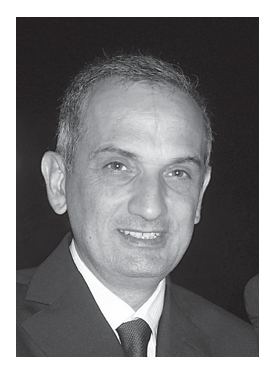
\includegraphics{graphics/Author_Bio/Domenico_Talia.eps}}{Photo of Domenico Talia.}[-130pt,23pt]
\vspace*{-18.5pt}
\end{wrapfigure} \textbf{Domenico Talia} is a full professor of computer engineering at the University of Calabria, Italy and an honorary professor at Amity University, Noida, India. He is co-founder of DtoK Lab. His research interests include Big Data analysis, cloud computing, machine learning, social data mining, parallel and distributed data analysis, mobile computing, and parallel programming.

He has published 12 books and more than 400 papers in archival journals such as \textit{CACM}, \hbox{\textit{Computer},} \textit{IEEE TKDE}, \textit{IEEE TSE}, \textit{IEEE TPDS}, \textit{IEEE} \textit{TSMC-B}, \textit{IEEE Micro}, \textit{ACM Computing Surveys}, \textit{FGCS}, \textit{\hbox{Parallel} \hbox{Computing}}, \textit{IEEE Internet Computing}, and international conference proceedings. He is a member of the editorial boards of \hbox{\textit{Computer},} \textit{IEEE Transactions on Parallel and Distributed Systems}, \textit{ACM Computing Surveys}, \textit{Future Generation Computer Systems}, \textit{Journal of Cloud Computing}, \textit{International\break Journal of Web and Grid Services}, \textit{Big Data and Cognitive Computing}, and \textit{Multiagent and Grid Systems}.

Prof. Talia has served as chair, organizer, or program committee member of several international conferences and given many invited talks, tutorials, and seminars in conferences and schools. He is a senior member of the ACM and IEEE.

A list of publications can be found here: \href{https://scholar.google.it/citations?user=domenicotalia}{https://{\allowbreak}scholar.{\allowbreak}google.it/{\allowbreak}citations?{\allowbreak}user={\allowbreak}domenicotalia}.



%\end{document}


%\include{ACM_Talia_Index}
 {\raggedright
 \printindex%%%%%%%% --
 }
\end{document}
